\pdfoutput=1\relax
\documentclass[reqno]{amsart}

\usepackage{verbatim}
\usepackage[textsize=scriptsize]{todonotes}
\usepackage{tikz-cd}
\usepackage{etoolbox}
\usepackage{etex}
\usepackage{hyperref}
\usepackage{cleveref}
\usepackage[T1]{fontenc}

%\hypersetup{
%    colorlinks,
%    linkcolor={red!30!black},
%    citecolor={blue!50!black},
%    urlcolor={blue!80!black}
%}

\usepackage{chemarr}
\usepackage{amssymb}
\usepackage{amsmath}
\usepackage{comment}
\usepackage{spectralsequences}
%\usepackage[draft]{spectralsequences}
\usepackage{cleveref}
\usepackage{mathtools}
\usepackage{rotating}
\usepackage{wrapfig}
\usepackage{outlines}
\usepackage{graphicx}
\usepackage{scalerel}
\def\DevnagVersion{2.17}
\usepackage{devanagari}
\usepackage{bbm}
\usepackage{multicol}

%For IPA symbols
\usepackage{tipa}

%----------------------------------------------------------------------%


\theoremstyle{definition}
\newtheorem{nul}{}[section]
\newtheorem{dfn}[nul]{Definition}
\newtheorem{axm}[nul]{Axiom}
\newtheorem{rmk}[nul]{Remark}
\newtheorem{term}[nul]{Terminology}
\newtheorem{cnstr}[nul]{Construction}
\newtheorem{cnv}[nul]{Convention}
\newtheorem{ntn}[nul]{Notation}
\newtheorem{exm}[nul]{Example}
\newtheorem{obs}[nul]{Observation}
\newtheorem{ctrexm}[nul]{Counterexample}
\newtheorem{rec}[nul]{Recollection}
\newtheorem{exr}[nul]{Exercise}
\newtheorem{wrn}[nul]{Warning}
\newtheorem{qst}[nul]{Question}
\newtheorem{prb}[nul]{Problem}
\newtheorem{ass}[nul]{Assumption}
\newtheorem*{dfn*}{Definition}
\newtheorem*{axm*}{Axiom}
\newtheorem*{ntn*}{Notation}
\newtheorem*{exm*}{Example}
\newtheorem*{exr*}{Exercise}
\newtheorem*{int*}{Intuition}
\newtheorem*{qst*}{Question}
\newtheorem*{rmk*}{Remark}
\newtheorem*{comp1}{Computation 1:}

\theoremstyle{plain}
\newtheorem{sch}[nul]{Scholium}
\newtheorem{claim}[nul]{Claim}
\newtheorem{thm}[nul]{Theorem}
\newtheorem{prop}[nul]{Proposition}
\newtheorem{summary}[nul]{Summary}
\newtheorem{lem}[nul]{Lemma}
\newtheorem{var}[nul]{Variant}
\newtheorem{sublem}{Lemma}[nul]
\newtheorem{por}[nul]{Porism}
\newtheorem{cnj}[nul]{Conjecture}
\newtheorem{cor}[nul]{Corollary}
\newtheorem{fact}[nul]{Fact}
\newtheorem*{thm*}{Theorem}
\newtheorem*{prop*}{Proposition}
\newtheorem*{cor*}{Corollary}
\newtheorem*{lem*}{Lemma}
\newtheorem*{cnj*}{Conjecture}
\newtheorem{innercustomthm}{Theorem}
\newenvironment{customthm}[1]
  {\renewcommand\theinnercustomthm{#1}\innercustomthm}
  {\endinnercustomthm}

%%% Make widetilde work in spectral sequences.

\let\oldwidetilde\widetilde
\protected\def\widetilde{\oldwidetilde}


%----------------------------------------------------------------------%

\DeclareMathOperator{\Aut}{\mathrm{Aut}}
\DeclareMathOperator{\Tr}{\mathrm{Tr}}
\DeclareMathOperator{\Res}{\mathrm{Res}}
\DeclareMathOperator{\im}{\mathrm{im}}
\DeclareMathOperator*{\colim}{\mathrm{colim}}
\DeclareMathOperator{\Map}{\mathrm{Map}}
\DeclareMathOperator{\cofiber}{\mathrm{cofiber}}
\DeclareMathOperator{\fiber}{\mathrm{fiber}}
\DeclareMathOperator{\gr}{\mathrm{gr}}
\DeclareMathOperator{\fib}{\mathrm{fib}}
\DeclareMathOperator{\sBar}{\mathrm{Bar}}

\DeclareMathOperator{\Hom}{\mathrm{Hom}} 
\DeclareMathOperator{\End}{\mathrm{End}} 
\DeclareMathOperator{\Skel}{\mathrm{Skel}}
\DeclareMathOperator*{\hocolim}{\mathrm{hocolim}}
\DeclareMathOperator*{\holim}{\mathrm{holim}}
\DeclareMathOperator{\smsh}{\wedge}
\DeclareMathOperator{\coker}{\mathrm{coker}}



\DeclareMathOperator{\Ss}{\mathbb{S}}
\DeclareMathOperator{\FF}{\mathbb{F}}
\DeclareMathOperator{\F}{\mathbb{F}}
%\DeclareMathOperator{\ZZ}{\mathbb{Z}}
\DeclareMathOperator{\QQ}{\mathbb{Q}}
\DeclareMathOperator{\NN}{\mathbb{N}}
\DeclareMathOperator{\A}{\mathcal{A}}
%\DeclareMathOperator{\C}{\mathcal{C}}
\DeclareMathOperator{\D}{\mathcal{D}}
\DeclareMathOperator{\CP}{\mathbb{CP}}
\DeclareMathOperator{\E}{\mathbb{E}}
\DeclareMathOperator{\sE}{\mathrm{E}}
\DeclareMathOperator{\mE}{\mathcal{E}}
\DeclareMathOperator{\MO}{\mathrm{MO}}
\DeclareMathOperator{\MOfn}{\mathrm{MO \langle 4m \rangle}}
\DeclareMathOperator{\MOn}{\mathrm{MO \langle n \rangle}}
\DeclareMathOperator{\MU}{\mathrm{MU}}
\DeclareMathOperator{\MUfn}{\mathrm{MU \langle 4n \rangle}}
%\DeclareMathOperator{\Of}{O \langle 4n-1\rangle}
%\DeclareMathOperator{\Uf}{U \langle 4n-1\rangle}
%\DeclareMathOperator{\spOf}{\Sigma^{\infty}_+ O \langle 4n-1\rangle}
%\DeclareMathOperator{\sOf}{\Sigma^{\infty} O \langle 4n-1\rangle}
%\DeclareMathOperator{\Of}{\mathrm{O} \langle 4n-1\rangle}
\DeclareMathOperator{\cS}{\mathcal{S}}
\DeclareMathOperator{\bS}{\mathbb{S}}
%\DeclareMathOperator{\Z}{\mathbb{Z}}
\DeclareMathOperator{\Ring}{\textbf{Ring}}
\DeclareMathOperator{\Aff}{\textbf{Aff}}
\DeclareMathOperator{\Ran}{\mathrm{Ran}}
\DeclareMathOperator{\Spec}{\mathrm{Spec}}
\DeclareMathOperator{\Poly}{\text{Poly}}
\DeclareMathOperator{\pic}{\mathrm{pic}}
\DeclareMathOperator{\Pic}{\mathrm{Pic}}
\DeclareMathOperator{\Fin}{\mathrm{Fin}}
\DeclareMathOperator{\Ext}{\mathrm{Ext}}
\DeclareMathOperator{\Gra}{\mathrm{Gr}}
\DeclareMathOperator{\nil}{\text{nil}}
\DeclareMathOperator{\ac}{\tilde{c}}
\DeclareMathOperator{\fin}{\text{fin}}
\DeclareMathOperator{\Gr}{\mathbf{Gr}}
\DeclareMathOperator{\Fil}{\mathbf{Fil}}
\DeclareMathOperator{\Fun}{\mathrm{Fun}}
\DeclareMathOperator{\Alg}{\mathrm{Alg}}
\DeclareMathOperator{\Sp}{\mathrm{Sp}}
\DeclareMathOperator{\Spaces}{\mathcal{S}}
\DeclareMathOperator{\J}{\mathcal{J}}
\DeclareMathOperator{\Cofil}{\mathbf{Cofil}}
\DeclareMathOperator{\GL}{\mathrm{GL}}
\DeclareMathOperator{\cofib}{\mathrm{cofib}}
\DeclareMathOperator{\cof}{\mathrm{cof}}
\DeclareMathOperator{\DD}{\mathbb{cofib}}
\DeclareMathOperator{\Sq}{\mathrm{Sq}}

\newcommand{\Of}{\mathrm{O \langle 4n-1\rangle}}
\newcommand{\Uf}{\mathrm{U \langle 4n-1\rangle}}
\newcommand{\spOf}{\Sigma^{\infty}_+ \mathrm{O \langle 4n-1\rangle}}
\newcommand{\spUf}{\Sigma^{\infty}_+ \mathrm{U \langle 4n-1\rangle}}
\newcommand{\sOf}{\Sigma^{\infty} \mathrm{O \langle 4m-1\rangle}}
\newcommand{\sUf}{\Sigma^{\infty} \mathrm{U \langle 4n-1\rangle}}
\newcommand{\wt}{\widetilde}
\newcommand{\BOn}{\mathrm{BO \langle n \rangle}}
\newcommand{\BOm}{\mathrm{BO \langle m \rangle}}
\newcommand{\BO}{\mathrm{BO}}
\newcommand{\Om}{\mathrm{O \langle m -1 \rangle}}
\newcommand{\Oo}{\mathrm{O}}
\newcommand{\U}{\mathrm{U}}
\newcommand{\BP}{\mathrm{BP}}
\newcommand{\Syn}{\mathrm{Syn}}
\newcommand{\HZ}{\mathrm{H}\mathbb{Z}}
\newcommand{\HF}{\mathbb{F}}
\newcommand{\HFp}{\mathbb{F}_p}
\newcommand{\Qoppa}{\kappa}
\newcommand{\qoppa}{\kappa}
\newcommand{\sampi}{\lambda}
\newcommand{\tor}{\mathrm{tor}}
\newcommand{\tf}{\mathrm{tf}}
\newcommand{\Tot}{\mathrm{Tot}}
\newcommand{\kappabar}{\overline{\kappa}}
\newcommand{\SO}{\mathrm{SO}}
\newcommand{\BSO}{\mathrm{BSO}}
\newcommand{\Str}{\mathrm{String}}
\newcommand{\MStr}{\mathrm{MString}}
\newcommand{\MOtw}{\mathrm{MO}\langle 12 \rangle}
\newcommand{\BStr}{\mathrm{BString}}
\newcommand{\Spin}{\mathrm{Spin}}
\newcommand{\MSpin}{\mathrm{MSpin}}
\newcommand{\ord}{\mathrm{ord}}
\newcommand{\MF}{\mathrm{MF}}
\newcommand{\tmf}{\mathrm{tmf}}
\newcommand{\Ah}{\widehat{A}}
%\newcommand{\CC}{\mathbb{C}}
\newcommand{\num}{\mathrm{num}}
\newcommand{\denom}{\mathrm{denom}}
\newcommand{\sig}{\mathrm{sig}}
\newcommand{\bp}{\mathrm{bP}}
\newcommand{\Z}{\mathbb{Z}}
\newcommand{\ZZ}{\mathbb{Z}}
\newcommand{\R}{\mathbb{R}}
\newcommand{\G}{\mathbb{G}}
\newcommand{\C}{\mathbb{C}}
\newcommand{\dtau}{\text{\scriptsize {\dn tO}}}
\newcommand{\ta}{\text{\footnotesize {\dn t}}}
\newcommand{\SHR}{\mathcal{SH}(\mathbb{R})}
\newcommand{\SHC}{\mathcal{SH}(\mathbb{C})}
\newcommand{\SH}{\mathcal{SH}}
\newcommand{\SHgc}{\mathcal{SH}(\mathbb{R})^{\scaleto{\mathrm{\bf \hspace{-1.5pt}A\hspace{-1.8pt}T}}{3.75pt}}_{i2}}
\newcommand{\Orb}{\mathrm{Orb}}
\newcommand{\Ft}{\mathbb{F}_2}
\newcommand{\Zt}{\mathbb{Z}_2}
\newcommand{\HFt}{\mathrm{M}\mathbb{F}_2}
\newcommand{\MFp}{\mathrm{M}\mathbb{F}_p}
\newcommand{\uFt}{\underline{\mathbb{F}}_2}
\newcommand{\HZt}{\mathrm{M}\mathbb{Z}_{2}}
\newcommand{\uZt}{\underline{\mathbb{Z}}_{2}}
\newcommand{\uZ}{\underline{\mathbb{Z}}}
\newcommand{\MGL}{\mathrm{MGL}}
\newcommand{\MUR}{\mathrm{MU}_{\mathbb{R}}}
\newcommand{\Mod}{\mathrm{Mod}}
\newcommand{\Triv}{\mathrm{Triv}}
\newcommand{\piu}{\underline{\pi}}
\newcommand{\En}{\mathbb{E}_n}
\newcommand{\CC}{\mathcal{C}}
\newcommand{\CCdef}{\mathcal{C}_{\mathrm{def}}}
\newcommand{\Comod}{\mathrm{Comod}}
\newcommand{\id}{\mathrm{id}}
\newcommand{\Ab}{\mathrm{Ab}}
\newcommand{\Abh}{\mathrm{Ab}^{\heartsuit}}
\newcommand{\uA}{\underline{\mathrm{A}}}
\newcommand{\uAb}{\underline{\mathrm{Ab}}}
\newcommand{\uAbh}{\underline{\mathrm{Ab}}^{\heartsuit}}
\newcommand{\ExtBP}{C^*_{\BP_{*}\BP}(\BP_{*})}
\newcommand{\ExtBPt}{C^*_{\BP_{2*}\BP}(\BP_{2*})}
\newcommand{\ExtBPtu}{\underline{C^*_{\BP_{2*}\BP}(\BP_{2*})}}

\def\Groth{\mathrm{Groth}}
\def\MUR{\mathrm{MU}_{\mathbb{R}}}
\def\MURu{\underline{\mathrm{MU}_{\mathbb{R}}}}
\def\MURpr{\mathrm{MU}_{\mathbb{R}}\mathrm{-proj}}
\def\MURev{\mathrm{MU}_{\mathbb{R},2}\mathrm{-even}}
\def\BPR{\mathrm{BP}_{\mathbb{R}}}
\def\BPRu{\underline{\mathrm{BP}_{\mathbb{R}}}}
\def\BPRpr{\mathrm{BP}_{\mathbb{R}}\mathrm{-proj}}
\def\BPRev{\mathrm{BP}_{\mathbb{R}}\mathrm{-even}}
\def\even{\mathrm{even}}
\def\twist{\mathrm{tw}}
\def\Mfg{\mathcal{M}_{\mathrm{fg}}}
\def\aut{\mathrm{Aut}}
\def\Ind{\mathrm{Ind}}
\def\QCoh{\mathrm{QCoh}}
\def\IndCoh{\mathrm{IndCoh}}
\def\spa{\mathrm{space}}

\def\SHCa{\mathcal{SH}(\mathbb{C})^{\scaleto{\mathrm{\bf \hspace{-1.5pt}A}}{3.75pt}}}
\def\SHCat{\mathcal{SH}(\mathbb{C})^{\scaleto{\mathrm{\bf \hspace{-1.5pt}A\hspace{-1.8pt}T}}{3.75pt}}_{ip}}

\def\SHk{\mathcal{SH}(k)}
\def\SHka{\mathcal{SH}(k)^{\scaleto{\mathrm{\bf \hspace{-1.5pt}A}}{3.75pt}}}
\def\SHkt{\mathcal{SH}(k)^{\scaleto{\mathrm{\bf \hspace{-1.5pt}T}}{3.75pt}}}
\def\SHkat{\mathcal{SH}(k)^{\scaleto{\mathrm{\bf \hspace{-1.5pt}A\hspace{-1.8pt}T}}{3.75pt}}}

\def\SHRa{\mathcal{SH}(\mathbb{R})^{\scaleto{\mathrm{\bf \hspace{-1.5pt}A}}{3.75pt}}}
\def\SHRt{\mathcal{SH}(\mathbb{R})^{\scaleto{\mathrm{\bf \hspace{-1.5pt}T}}{3.75pt}}}
\def\SHRat{\mathcal{SH}(\mathbb{R})^{\scaleto{\mathrm{\bf \hspace{-1.5pt}A\hspace{-1.8pt}T}}{3.75pt}}_{i2}}
\def\SHRatch{\mathcal{SH}(\mathbb{R})^{\scaleto{\mathrm{\bf \hspace{-1.5pt}A\hspace{-1.8pt}T}}{3.75pt}, \mathrm{C}-\heartsuit}_{i2}}

\def\slice{\mathrm{slice}}
\def\cb{\mathrm{cb}}
\def\diag{\mathrm{Diag}}
\def\Q{\mathbb{Q}}
\def\RP{\mathbb{RP}}
\def\KO{\mathrm{KO}}
\def\KQ{\mathrm{KQ}}
\def\KGL{\mathrm{KGL}}
\def\DM{\mathrm{DM}}
\def\nuc{\nu_{\mathbb{C}}}
\def\nur{\nu_{\mathbb{R}}}
\def\TMF{\mathrm{TMF}}
\def\uHom{\underline{\mathrm{Hom}}}
\def\th{\otimes-\heartsuit}
\def\ch{\mathrm{C}-\heartsuit}
\def\cn{\mathrm{C}}
\def\at{\scaleto{\mathrm{\bf \hspace{-1.5pt}A\hspace{-1.8pt}T}}{3.75pt}}
\def\att{\scaleto{\mathrm{\bf A\hspace{-1.8pt}T}}{3.75pt}}
\def\gceff{\scaleto{\mathrm{\bf A\hspace{-1.8pt}T}}{3.75pt}\mathrm{-eff}}
\def\eff{\mathrm{eff}}
\def\Sm{\textbf{Sm}}
\def\cell{\mathrm{cell}}
\def\ko{\mathrm{ko}}
\def\ku{\mathrm{ku}}
\def\res{\mathrm{res}}
\def\triv{\mathrm{triv}}
\def\kq{\mathrm{kq}}
\def\kgl{\mathrm{kgl}}
\def\CAlg{\mathrm{CAlg}}
\def\o{\mathbbm{1}}
\def\Re{\mathrm{Re}}
\def\MR{\mathrm{Mot}_{\mathbb{R}}}
\def\MC{\mathrm{Mot}_{\mathbb{C}}}
\def\b{\mathrm{Be}}
\def\H{\mathrm{H}}
\def\sp{S^{\wedge}_{p}}
\def\P{\mathbb{P}}
\def\AA{\mathbb{A}}
%\DeclareSymbolFont{extraitalic}      {U}{zavm}{m}{it}
%\DeclareMathSymbol{\Qoppa}{\mathord}{extraitalic}{161}
%\DeclareMathSymbol{\qoppa}{\mathord}{extraitalic}{161}
%\DeclareMathSymbol{\sampi}{\mathord}{extraitalic}{166}

\DeclarePairedDelimiter\abs{\lvert}{\rvert}%
\makeatletter
\let\oldabs\abs
\def\abs{\@ifstar{\oldabs}{\oldabs*}}

%%% Code from Hood to fix a positioning error with his spectralsequences package.
%% \usepackage{etoolbox}
%% \makeatletter
%% \patchcmd\endsseqpage{\path (0,-\sseq@yoffset) node}{\node}{}{\failed}
%% \makeatother


%----------------------------------------------------------------------%

\usepackage{tikz}
\usetikzlibrary{matrix,arrows,decorations}
\usepackage{tikz-cd}

\usepackage{adjustbox}

\let\oldtocsection=\tocsection
 
\let\oldtocsubsection=\tocsubsection
 
\let\oldtocsubsubsection=\tocsubsubsection
 
\renewcommand{\tocsection}[2]{\hspace{0em}\oldtocsection{#1}{#2}}
\renewcommand{\tocsubsection}[2]{\hspace{1em}\oldtocsubsection{#1}{#2}}
\renewcommand{\tocsubsubsection}[2]{\hspace{2em}\oldtocsubsubsection{#1}{#2}}

%----------------------------------------------------------------------%
%%% Local Variables:
%%% mode: latex
%%% TeX-master: "Main"
%%% eval: (visual-line-mode t)
%%% eval: (auto-fill-mode 0)
%%% End:


\usepackage{etoolbox}
\newtoggle{draft}
% NB: toggle this to hide comments
\togglefalse{draft}
%\toggletrue{draft}

\iftoggle{draft} {
\usepackage[margin=1.5in]{geometry}
\newcommand{\NB}[1]{\todo[color=gray!40]{#1}}
\newcommand{\TODO}[1]{\todo[color=red]{#1}}
}{ % else
\usepackage[margin=1.5in]{geometry}
\newcommand{\NB}[1]{}
\newcommand{\TODO}[1]{}
\renewcommand{\todo}[1]{}
\renewcommand{\todo}[1]{}
}
\geometry{a4paper}

\title{Galois reconstruction of Artin--Tate $\R$-motivic spectra}
%\date{\today}

\author{Robert Burklund}
\address{Department of Mathematics, MIT, Cambridge, MA, USA}
\email{burklund@mit.edu}

\author{Jeremy Hahn}
\address{Department of Mathematics, MIT, Cambridge, MA, USA}
\email{jhahn01@mit.edu}

\author{Andrew Senger}
%\thanks{During the course of this work, the third author was supported by an NSF GRFP fellowship under Grant No. 1122374.}
\address{Department of Mathematics, Harvard University, Cambridge, MA, USA}
\email{senger@math.harvard.edu}


%----------------------------------------------------------------------%
%----------------------------------------------------------------------%

\begin{document}
\begin{abstract}
We explain how to reconstruct the category of Artin--Tate $\R$-motivic spectra as a deformation of the purely topological $C_2$-equivariant stable category.
The special fiber of this deformation is algebraic,
and equivalent to an appropriate category of $C_2$-equivariant sheaves on the moduli stack of formal groups.
%% and controlled by the $\mathrm{E}_1$-page of the slice spectral sequence for the trigraded homotopy groups of the motivic sphere.
As such, our results directly generalize the cofiber of $\tau$ philosophy that has revolutionized classical stable homotopy theory.

A key observation is that the Artin--Tate subcategory of $\R$-motivic spectra is easier to understand than the previously studied cellular subcategory.
In particular, the Artin--Tate category contains a variant of the $\tau$ map, which is a feature conspicuously absent from the cellular category.
%% We explore a network of functors connecting the Artin--Tate $\R$-motivic, cellular $\C$-motivic, $C_2$-equivariant, and classical stable homotopy theories.

%  We suffer through completion issues. Why colim lim no commute. :(
\end{abstract}
\maketitle

\setcounter{tocdepth}{1}
\tableofcontents
\vbadness 5000

%----------------------------------------------------------------------%

% \newpage
\section{Introduction} \label{sec:intro}
%% Motivic homotopy theory, as introduced by Morel and Voevodsky \cite{MorelVoevodsky}, has been a tremendously successful application of abstract homotopy theory to concrete questions of algebraic geometry and number theory. \todo{This sentence is stolen from Gheorghe--Wang--Xu. It should be rewritten.}

A striking surprise of modern computational stable homotopy theory is that the category $\SH(\C)$ of $\C$-motivic spectra, as introduced by Morel and Voevodsky \cite{MorelVoevodsky},
has found use not only in algebraic geometry, but also in the computation of stable homotopy groups of spheres, a question of purely topological origin.  In particular, the $p$-completed bi-graded homotopy groups of the unit in $\SH(\C)$ record---in a precise sense---the Adams--Novikov spectral sequence for the sphere spectrum, including all differentials and extensions.  The ultimate expression of this connection is the discovery that the \emph{cellular} subcategory of $p$-complete $\C$-motivic spectra is equivalent to a category of \emph{synthetic} Adams--Novikov spectral sequences, and in particular has a purely homotopy theoretic description without reference to algebraic geometry.

%% The relationship between $p$-complete, cellular $\C$-motivic spectra and Adams--Novikov spectral sequences is mediated by a class $\tau:\Ss^1 \to (\G_m)^{\wedge}_p$.  The cofiber of the $\tau$ map (often denoted $C\tau$) is an $\mathbb{E}_\infty$-algebra, with the property that cellular $C\tau$-modules record the purely algebraic derived category of $p$-complete $\BP_*\BP$-comodules.  On the other hand, the full subcategory of $\tau$-invertible, $p$-complete motivic $\C$-spectra is equivalent to the classical category of $p$-complete spectra.  One summarizes the situation by saying that $\SH(\C)^{cell,p}$ is a $\tau$-deformation, with generic fiber the category of $p$-complete spectra and special fiber the derived category of $p$-complete $\BP_*\BP$-comodules.

The first evidence that a large sector of the motivic category contains only topological information appears in the work of Thomason on algebraic K-theory and \'etale cohomology \cite{Thomason}. As a consequence of this work, Thomason proves that for well-behaved $\C$-schemes $X$, there is an equivalence $\mathrm{K}^{\mathrm{alg}} (X) [\beta^{-1}]^{\wedge} _{\ell} \simeq \mathrm{KU} (X(\C))^{\wedge} _{\ell}$, where $\beta$ is a certain Bott element. %% There is a precise sense in which inverting $\beta$ is equivalent to inverting $\tau$.
These ideas have been refined over the years, culminating in the following theorem.

\begin{thm}[\cite{VoeOpenProbs, DI, LevineComparison, LevineSlicemU, Ctau, ctauactalol, Pstragowski, cmmf}]\label{thm:C-main}\

  In $\SHC$
  there is a map $\tau : \Ss^1 \to (\G_m)_p$
  which enjoys the following properties:
  \begin{enumerate}
  \item[(1.\hspace{1em}]\hspace{-1.1em}$\mathrm{Generically\ Topological})$ The full subcategory of $\tau$-local objects in $\SHC^{cell}_p$ is equivalent to $\Sp_p$.
  \item[(2.\hspace{1em}]\hspace{-1.1em}$\mathrm{Algebraic\ Degeneration})$ The cofiber of $\tau$ (often denoted $C\tau$) is a commutative algebra, and the category of dualizable modules over $C\tau$ is equivalent to the category of $p$-completions of dualizable objects in $\QCoh(\mathcal{M}_{\mathrm{fg}})$, where $\Mfg$ is the moduli stack of formal groups.
  \item[(3.\hspace{1em}]\hspace{-1.1em}$\mathrm{Galois\ Reconstruction})$ There is a purely topological construction of $\SHC_p^{cell}$.
  \end{enumerate}
  
  We summarize this situation by saying that $\SH(\C)_p^{cell}$ is a $1$-parameter deformation of $p$-complete spectra with parameter $\tau$ and a purely algebraic special fiber.
\end{thm}

Although it does not appear in the statement, understanding the algebraic cobordism spectrum, $\MGL$, is key to proving this theorem. 
The importance of $\MGL$ to the study of cellular motivic spectra goes back to Voevodsky's work on the effective slice filtration \cite{VoeOpenProbs}.
In that work, Voevosky conjectured that the effective slice filtration of the unit over an algebraically closed field 
may be described in terms of the Adams-Novikov spectral sequence. 
%% may be described in terms of the $\mathrm{E}_2$-page of the Adams-Novikov spectral sequence and further suggested a relationship between the effective slice spectral sequence of the unit over an algebraically closed field and the Adams-Novikov spectral sequence.
Levine later proved Voevodsky's conjectures \cite{LevineComparison, LevineSlicemU}.
Voevodsky's notion of ``rigid homotopy groups'' also foreshadowed \emph{algebraic degeneration}.
In this framework he and Rezk predicted that the rigid Adams spectral sequence is equivalent to the algebraic Novikov spectral sequence \cite[p. 20-21]{VoeOpenProbs}, a result later proven in different language by Gheorghe--Wang--Xu \cite[Theorem 1.17]{ctauactalol}.
The fact that the category of $p$-complete $\C$-motivic spectra is \emph{generically topological} is strongly suggested by results of Dugger--Isaksen \cite[Section 2.6]{DI}, though to the best of our knowledge the full result did not appear in print until \cite{Pstragowski}.\todo{I can't find an earlier one at least, but that could easily just be me. Piotr does beat Tom's etale rigidity paper.}
The commutative algebra structure on $C\tau$ was first constructed by Gheorghe \cite{Ctau},
and the category of modules over $C\tau$ was then identified by Gheorghe--Wang--Xu in \cite{ctauactalol}.
Finally, % \emph{Galois reconstruction} was accomplished independently by 
Pstragowski \cite{Pstragowski} and Gheorghe--Isaksen--Krause--Ricka \cite{cmmf}
independently provided two different \emph{Galois reconstructions} of cellular $p$-complete $\C$-motivic spectra. %% moreover, \cite{Pstragowski} reproves (2) independently of \cite{Ctau} and \cite{ctauactalol}.

%% In SECTION, we show that there is a precise dictionary between Voevodsky's language of the effective slice filtration and rigid homotopy groups, and the language used in \Cref{thm:C-main}.

With the case of $\C$ resolved we raise the following natural question:

\begin{qst}\label{qst:main}
  To what extent can this theorem be extended to a general field $k$?
\end{qst}

As stated, this question is too imprecise to admit a definitive answer, so we begin by refining two points of ambiguity: the appropriate subcategory of $\SHk$ one should consider and the meaning of purely topological. In our study of this question we have found that the appropriate subcategory is the category of Artin--Tate motivic spectra (defined below). Notably, over $\R$, if one restricts to the further subcategory of cellular objects, it becomes significantly more difficult to construct a topological model.

\begin{dfn}
  The category of Artin--Tate motivic spectra over $k$ is the smallest stable full subcategory
  $\SHkat \subset \SHk$,
  closed under tensor products and colimits, that contains the motives of finite \'etale $k$-algebras, 
  $\P_k^1$ and $(\P_k^1)^{-1}$.
\end{dfn}

The phrase `purely topological' has a double meaning.
On the one hand it refers to the input to the construction;
it should not depend directly on the arithmetic of $k$, instead using only the absolute Galois group, $G$, together with the character $G \to \widehat{\Z}^\times$ induced by the maximal cyclotomic extension of $k$ \footnote{More specifically, the $p$-complete category should only depend on the $\Z_p^\times$ component of this map.}.
On the other hand it asks for a construction which uses only the ``standard machinery of homotopy theory.''

The authors are not the first to take up questions of this nature.
%% Indeed, beyond the work by many authors in the case $k = \C$ discussed above,
Positselski has studied the question of Galois reconstruction for the category $\DM(k;\F_\ell)^{\at}$ of mixed Artin-Tate motives with mod $\ell$ coefficients \cite{DMRecon,GalKosz}. With a few exceptions, he has shown that when $k$ is a finite, local or global field, then $\DM(k,\F_\ell)^{\at}$ may be viewed as a derived category of filtered discrete $G$-modules with restricted sub-quotients. %the restriction being given in terms of the cyclotomic character.

In a different direction, work of Bachmann, Elmanto and {\O}stv{\ae}r shows that, up to a completion, $\SH(S)$ is generically \'etale for a wide range of schemes $S$ \cite{TomEtaleI, TomEtaleII}. In particular, Bachmann--Elmanto--{\O}stv{\ae}r show that, after a suitable completion, \'etale localization corresponds to inverting $\tau$. Note that $\tau$ may not exist in the homotopy of the completed unit, so care must be taken to interpret this statement.
Furthermore, Bachmann showed that, again up to completion, the \'etale motivic category is equivalent to the category of hypercomplete sheaves of spectra on the small \'etale site.
Specializing to the case $S = \Spec k$, we find that, up to completion, the category of $\tau$-local objects in $\SH(k)$ admits a description in terms of Borel $G$-equivariant spectra.

Previously, work of Behrens and Shah \cite{BehrensShah} had taken up the question of when a suitable map $\tau$ exists over $\R$. 
Although there is no map $\tau:\Ss^1 \to (\G_m)^{\wedge}_2$ in $\SH(\R)$,
%% though such a class does exist after tensoring with the spectrum $\HFt$ representing mod $2$ motivic cohomology.
they prove that $\tau$ exists whenever a different class $\rho:\Ss^0 \to \G_m$ has been killed.
If only $\rho^2$ is killed, but not $\rho$ itself, then $\tau$ does not necessarily exist, but $\tau^2$ does.
Continuing in this way, they make sense of inverting $\tau$ in any $\rho$-complete situation.
%% but the resulting $\tau$-inverted objects are more closely related to Borel $C_2$-spectra than genuine $C_2$-spectra.
%% Furthermore, there is no way to construct $C\tau$ without first killing $\rho$. This makes it impossible to describe cellular $\R$-motivic spectra as a $\tau$-deformation.

%% \todo{What's below needs to be joined up with what's above.}

%% In recent years the category $\SHR$ of $\R$-motivic spectra has similarly been found to shed light on the genuine $C_2$-equivariant stable homotopy category.  However, the exact relationship between $\R$-motivic stems and any sort of equivariant Adams--Novikov spectral sequence has remained mysterious, and before the present work there has been no purely homotopy theoretic construction of the cellular subcategory of $\SH(\R)$.

In this paper we resolve \Cref{qst:main} in the case $k=\R$.
This begins with the observation that if one does not insist that the target of $\tau$ must be a completion of $\G_m$, then a suitable replacement can easily be constructed.
%% The first 
%% The main moral of this paper is that all of these subtleties disappear so long as one is willing to consider grading $\R$-motivic homotopy groups not just by the Picard elements $\Ss^1$ and $\mathbb{G}_m$, but also by a third Picard element $\Ss^{\C}$.  Here, $\Ss^{\C}$ is the suspension spectrum of the unreduced suspension of $\Spec(\C)$.

\begin{thm}\label{thm:main}
  In $\SHRat$
  there is an invertible object $Q$ and a map $\ta : \Ss^1 \to Q_2$
  which enjoys the following properties:%\footnote{As we will explain in our conventions below, we use $\SHRat$ to denote the category of modules over the $2$-completion of the unit in $\SHR^{\at}$.}
  \begin{enumerate}
  \item[(GT)] The full subcategory of $\ta$-local objects in $\SHR^{\at}_{i2}$ is equivalent to $\Sp_{C_2,i2}$.
  \item[(AD)] The cofiber of $\ta$ (denoted $C\ta$) is a commutative algebra, and the category of dualizable modules over $C\ta$ is equivalent to the category of dualizable objects in the derived category of Mackey-functor $\MU_*\MU$-comodules \footnote{See \Cref{sec:cta} for a precise definition of this category.}.
  \item[(GR)] There is a purely topological construction of $\SHRat$.
    In particular, we construct a commutative algebra $R_\bullet$ in filtered, $C_2$-equivariant spectra
    such that the category of filtered modules over $R_\bullet$ is equivalent to $\SHRat$.
    The commutative algebra $R_\bullet$ is the even slice--d\'ecalage of the $\MUR$-Adams tower for the sphere \footnote{See \Cref{sec:top} for precise definitions.}.    
  \end{enumerate}
  
  We summarize this by saying that $\SHR^{\at}_{i2}$ is a $1$-parameter deformation of $C_2$-equivariant stable homotopy theory with parameter $\ta$ and purely algebraic special fiber.
\end{thm}

The romanization of the Devanagari letter $\ta$ is `ta' \footnote{However, the reader who is not familiar with the Devanagari alphabet is advised that the pronunciation of $\ta$ in the majority of South Asian languages using Devanagari is given in IPA by /\textsubbridge{t}\textschwa/, which is closer to `tuh' in English than `ta.'}  and
our choice of this symbol will be explained in \Cref{rmk:ta-explanation}. As in the case over $\C$, we are also able to give an explicit formula for the homotopy groups of $C\ta$, though since we have not yet set up the appropriate notion of homotopy groups we will defer an explicit statement until later.
%% Note that the $p$-completions present in the theorem statement are necessary.
The subscript $i2$ appearing in the theorem statement refers to the category of modules over the $2$-completion of the unit. 
The reader who is worried by this departure from the norm may wish to read the section on notations and conventions before proceeding.
%% about the handling of $p$-completion may wish to read \Cref{app:completion} which sets up our general approach to completion issues before proceeding.

\ 

With the resolution of \Cref{qst:main} in the case of $\R$, the authors are hopeful that we might see this question resolved in its entirety in the near future.

%% \begin{cnstr}
%% There is a canonical class $\ta: \Ss^{\C} \to (\G_m)^{\wedge}_2$.  We will build $\ta$ in \Cref{sec:tau} via the explicit algebraic geometry of the circle $Q=\Spec \R[x,y]/(x^2+y^2-1)$.  A key point is that $\Sigma^{\infty} Q$ is itself a Picard element in $\SHgc$, satisfying a relation $\Ss^{\C} \otimes \Sigma^{\infty} Q \simeq \Ss^1 \otimes \G_m$.
%% \end{cnstr

%% \begin{rmk}
%%   The romanization of the Devanagari letter $\ta$ is `ta.' \footnote{However, the reader who does not know Hindi or another language which utilizes the the Devanagari alphabet should be advised that its pronunciation is closer to `tuh.' To be even more correct, the `t' sound should be dental and unaspirated.}  As we will explain in \Cref{sec:homology}, our choice of this character arises from the fact that there is a class $u:\Ss^1 \otimes (\Ss^{\C})^{-1} \to \HFt$ and a product relation $\ta u = \tau \in \pi_{***}^{\R}(\HFt).$    In other words, ta $\cdot$ u is tau.
	
%% It follows that inverting $\tau$ is the same as inverting both $\ta$ and $u$.  We have shown that inverting $\ta$ is equivalent to Betti realization, while inverting $u$ Borel completes genuine $C_2$ spectra.


\subsection{Examples of Artin--Tate motivic spectra}\ 

In this subsection, which is preparatory to all later material, we give a more comprehensive introduction to the category of Artin--Tate motivic spectra over a field. This begins with introducing the smaller subcategories of Artin and Tate objects, which together generate the category of Artin--Tate objects. The bulk of the subsection is spent building a collection of important examples of Artin--Tate motivic spectra. Over $\R$ a special role is played by the invertible objects and so we focus specific attention there. We close the section by discussing homotopy groups.

\begin{dfn}
  The categories of Artin, Tate and Artin--Tate motivic spectra over $k$ are the stable, full subcategories of $\SHk$, closed under tensor products and colimits, with the following generators:
  \begin{itemize}
  \item The category of Artin motivic spectra, $\SHka$, is generated by the motives of finite \'etale $k$-algebras.
  \item The category of Tate motivic spectra, $\SHkt$, is generated by the motives of $\P_k^1$ and $(\P_k^1)^{-1}$ \footnote{This category is sometimes referred to as the cellular category following \cite{DICell}.}.
  \item The category of Artin--Tate motivic spectra, $\SHkat$, is generated by the motives of finite \'etale $k$-algebras together with $\P_k^1$ and $(\P_k^1)^{-1}$.
  \end{itemize}
  Since these subcategories are closed under tensor products and colimits, they each inherit the structure of a stable, presentably symmetric monoidal category from $\SHk$. \footnote{In the sequel, we will state without remark results that are only known to be true after the characteristic of $k$ is inverted. The reader is invited to restrict themself to $k$ of characteristic zero if they prefer.}
\end{dfn}

We now turn to examples of objects in each of these categories, starting with the trivial and heading towards the non-trival.

\begin{exm} \label{exm:Sp-unit}
  Every stable, presentably symmetric monoidal category admits a unique symmetric monoidal functor from the category of spectra \cite[Corollary 4.8.2.19]{HA} \footnote{Another way of saying this is that $\Sp$ is the initial object of $\mathrm{CAlg}(Pr^{L,\mathrm{stab}})$.}.
  This gives us objects $X \otimes \o_k$ for every spectrum $X$.
  Of particular interest are the integer simplicial suspensions of the unit, $\Ss^{n} \otimes \o_k$.
\end{exm}

Inductively applying the homotopy purity theorem \cite[Theorem 3.2.23]{MorelVoevodsky} to the decomposition $\P^n _k = \mathbb{A}^{n} _k \coprod \P^{n-1} _k$, we learn that:

\begin{exm}[{\cite[Example 2.12]{DICell}}]
  For each $n$, the motivic spectrum associated to $\P^n_k$ is Tate.
\end{exm}

More generally, using a Bialynicki-Birula decomposition, Wendt shows that any smooth projective variety which admits a $\G_m$-action whose fixed points are discrete and rational is Tate \cite{Wendt} \footnote{In the case where the fixed points are not rational, the authors wonder what conditions are necessary to guarantees the motive is Artin--Tate.}.

\begin{exm}[{\cite[Theorem 6.4]{DICell}, \cite[Proposition 8.1]{HM}, \cite[Proposition 8.12]{etaPeriodic}}]
  Each of the following commutative algebras is Tate:
  \[ \MGL,\quad \kq,\quad \kgl,\quad \mathrm{M}\Z,\quad \mathrm{M}\F_p. \]
\end{exm}

\begin{exm} \label{exm:galois-corr}
  Essentially by definition, the Galois correspondence provides functors
  \begin{center}
    \begin{tikzcd}
      {\left\{ \footnotesize\parbox{2.25cm}{finite, continuous Gal($\overline{k}/k$)-sets} \right\}} \ar[r] &
      {\left\{ \footnotesize\parbox{1.5cm}{finite, etale $k$-algebras} \right\}^{op}} \ar[r, hook] \ar[d] &
      \mathrm{Sm}_k \ar[d] \\
      & \SHka \ar[r, hook] &
      \SHk,
    \end{tikzcd}
  \end{center}
  which give our first examples of Artin objects.
\end{exm}

Since the functor in the example above sends disjoint unions to sums there is no loss in generality if we restrict to transitive Gal($\overline{k}/k$)-sets (field extensions). In the case of $\R$ this gives only two objects: $\Spec(\R)$, which we will temporarily denote $\o_\R$ since is it the monoidal unit of the category, and $\Spec(\C)$. Using the natural map we get a cofiber sequence
\begin{align} \Spec(\C) \to \o_\R \xrightarrow{a} \Ss^{\C}. \label{eq:pic-C} \end{align}
On the level of $\C$-points (with Galois action), this cofiber sequence gives the representation sphere $\Ss^{\sigma}$.




Given a quadric in the plane, $V$, we can take its closure in $\P_k^2$ to obtain $\overline{V}$ which is a form of $\P_k^1$. If we let $x_1,\dots,x_n$ denote the points at infinity, then by the homotopy purity theorem \cite[Theorem 3.2.23]{MorelVoevodsky} we have a cofiber sequence
\[ V \to \overline{V} \to \bigoplus_{i=1,\dots,n} \P_{k(x_i)}^1. \]
Under the assumption that $V$ admits a rational point, $\overline{V}$ is just $\P^1_k$, and so we obtain our first non-trivial example of a motive which is neither Artin nor Tate, but is Artin--Tate:

\begin{exm}
  The motive of an affine quadric which admits a rational point is Artin--Tate.
\end{exm}

Over $\R$ there is a particular affine quadric of interest to us.
It is the object $Q$ which appeared in the statement of \Cref{thm:main}.

\begin{exm}
  Let $Q \coloneqq \{x^2+y^2=1\} \subset \AA^2 _{\R}$, which we shall call the algebraic circle.
  %% From the previous example we know that $Q$ is Artin--Tate.
  $Q$ has the additional property that it is a form of $\G_m$ \footnote{By Cartier duality, forms of $\G_m$ are classified by rank 1 lattices with Galois action. $Q$ corresponds to the unique nontrival action.}.
  Its group scheme structure comes from the usual rule for multiplication of complex numbers,
  namely
  \[ (x_1,y_1) \cdot (x_2,y_2) = (x_1 x_2 - y_1 y_2,\ x_1 y_2 + y_1 x_2). \]
  %% Furthermore, it is a form of $\G_m$---there is an isomorphism $(Q)_\C \cong (\G_m)_\C$ of commutative group schemes over $\C$.

  In \Cref{sec:ta} we will construct the maps $\ta: \Ss^1 \to Q_p$ using our explicit understanding of this group scheme.
\end{exm}

\begin{prop}[{\cite[Proposition 1.1]{HuPicard}}] \label{prop:pic-Q}
  There is an equivalence $Q \otimes \Ss^\C \simeq \P^1 _\R$.
  In particular, both $\Ss^\C$ and $Q$ are invertible.
\end{prop}

At this point we are ready to define the appropriate notion of homotopy groups for studying $\SHR^{\at}$.
In the case of $\SHC^{\at}$, the category has a bi-graded family of compact invertible generators given by the spheres $\Ss^{p - 2w} \otimes (\P_\C^1)^{\otimes w}$. Therefore, it is typical to study objects at the level of their bigraded homotopy groups, given by
\[ \pi_{p,w}^\C(X) \coloneqq \pi_0\Map ( \Ss^{p-2w} \otimes (\P_\C^1)^{\otimes w}, X ). \]
Similarly, $\SHRt$ has a bi-graded family of compact invertible generators given by the spheres $\Ss^{p-2w} \otimes (\P_\R^1)^{\otimes w}$, and it is typical to study objects through their bi-graded homotopy groups.
Using \Cref{prop:pic-Q} and \Cref{eq:pic-C}, the category $\SHR^{\at}$ has a tri-graded family of compact invertible generators given by the spheres $\Ss^{p-w} \otimes (\Ss^\C)^{\otimes q-w} \otimes (\P_\R^1)^{\otimes w}$, and we will study most objects through their tri-graded homotopy groups.

\begin{ntn}
  We endow the categories $\Sp$, $\Sp_{C_2}$, $\SHC$ and $\SHR$ with Picard gradings by spheres as follows:
  \begin{center}
    \renewcommand{\arraystretch}{1.1}
    \begin{tabular}{|l|l|l|} \hline
      Category & Picard & Spheres \\\hline\hline
      $\Sp$ & $\Z$ & $\Ss^p \simeq (S^1)^{\otimes p}$ \\\hline
      $\Sp_{C_2}$ & $\Z \times \Z$ & $\Ss^{p+q\sigma} \simeq (S^1)^{\otimes p} \otimes (S^\sigma)^{\otimes q}$ \\\hline
      $\SHC$ & $\Z \times \Z$ & $\Ss^{p,w} \simeq (S^1)^{\otimes p-2w} \otimes (\P_\C^1)^{\otimes w}$ \\\hline
      $\SHR$ & $\Z \times \Z \times \Z$ & $\Ss^{p,q,w} \simeq (S^1)^{\otimes p-w} \otimes (S^\C)^{\otimes q-w} \otimes (\P_\R^1)^{\otimes w}$ \\\hline
    \end{tabular}
    \renewcommand{\arraystretch}{1.0}
  \end{center}
  
  For any $p,q,w \in \Z$, and any $\R$-motivic spectrum $X$, we let $\pi^{\R}_{p,q,w} X$ denote the group of homotopy classes of maps,
  \[ (S^1)^{\otimes p-w} \otimes (S^\C)^{\otimes q-w} \otimes (\P_\R^1)^{\otimes w} \to X. \]
\end{ntn}

\begin{exm}
  For convenience we record what the invertible objects considered in this section look like under this new notation:
  \begin{center}
    \begin{tabular}{ccc}   
      $\Ss^{0,0,0} \cong \o_\R$ \qquad\qquad\qquad &
      $\Ss^{1,0,0} \cong S^1$ \qquad\qquad\qquad & 
      $\Ss^{0,1,0} \cong S^{\C}$ \\
      $\Ss^{0,1,1} \cong \G_m$ \qquad\qquad\qquad &
      $\Ss^{1,0,1} \cong Q$ \qquad\qquad\qquad &
      $\Ss^{1,1,1} \cong \P_\R^1$
    \end{tabular}
  \end{center}
  In the case of $\Ss^{0,0,0}$ we will often drop the indices for brevity, writing only $\Ss$.
  The two maps between Picard elements considered thus far, $\ta$ and $a$, become
  \[ \ta \in \pi_{0,0,-1}^\R \Ss_p \qquad\quad \text{ and } \qquad\quad a \in \pi_{0,-1,0}^\R \Ss. \]
  %% In the case when $X$ is the unit we will often omit it from the notation for brevity.
\end{exm}

\begin{rmk}
  The tri-graded spheres in $\SHR^{\at}$ which are Tate are precisely the spheres of the form $\Ss^{p,q,q}$.
  For this reason the Tate category only sees a `slice' of the total information present in the tri-graded homotopy groups.

  The tri-graded spheres in $\SHR^{\at}$ which are Artin are precisely the spheres of the form $\Ss^{p,q,0}$.
  The Artin category similarly only sees a `slice' of the total homotopy groups.

  %% Traditionally, $\SHR$ is viewed as bigraded by the spheres $\Ss^{p,w} \simeq (S^1)^{\otimes p-w} \otimes (\G_m)^{w}$. The comparison with our trigraded spheres is given by the equivalence $\Ss^{p,w} \simeq \Ss^{p-w,w,w}$, and from this we see that the bigraded sheres capture precisely those trigraded spheres $\Ss^{p,q,w}$ satisfying $q=w$.
\end{rmk}

%% as a  defined by [people]. We regard this category as the correct analog of the category over cellular objects over an algebraically closed field and propose that it may be possible to extend the full package of results known in the cellular case over algebraically closed fields to the Artin-Tate category over general fields. 


%% the the Picard elements $\Ss^1$, $\G_m$, $\Ss^{\C}$ and their inverses.

%% Let $\Ss_2^{\wedge}$ denote the $2$-completed unit in $\SHR$, and consider the category $\Ss_2^{\wedge}$-mod of $\Ss_2^{\wedge}$-module spectra.  We similarly define $\SHgc_2$ to be the smallest full subcategory of $\Ss_2^{\wedge}$-mod, closed under colimits and tensor products over $\Ss^{\wedge}_{2}$, containing the Picard elements $(\Ss^1)^{\wedge}_2, (\G_m)_2^{\wedge}$, $(\Ss^{\C})_2^{\wedge}$, and their inverses.

%% Both $\SHgc$ and $\SHgc_2$ are symmetric monoidal stable $\infty$-categories, and by CITE the $2$-completions of these categories are equivalent.  Note however that not every object in $\SHgc_2$ is $2$-complete.
%% \end{dfn}


%% \begin{cnstr}
%% There is a canonical class $\ta: \Ss^{\C} \to (\G_m)^{\wedge}_2$.  We will build $\ta$ in \Cref{sec:tau} via the explicit algebraic geometry of the circle $Q=\Spec \R[x,y]/(x^2+y^2-1)$.  A key point is that $\Sigma^{\infty} Q$ is itself a Picard element in $\SHgc$, satisfying a relation $\Ss^{\C} \otimes \Sigma^{\infty} Q \simeq \Ss^1 \otimes \G_m$.
%% \end{cnstr}


%% In this section, we introduce some exotic Picard elements in $\SHR$, use them to define trigraded homotopy groups, and define some maps between them, in particular the element $\ta \in \pi^{\R} _{0,0,-1} \Ss_p$, which serves as a Picard-graded analogue of the class $\tau \in \pi^{\C} _{0,-1} \Ss_p$.

%% \todo{Give a general definition of things}
%% \todo{Conjecture: every pic element is already in this category}

%% We discuss Picard gradings in $\Sp$, $\Sp_{C_2}$, $\SHC$ and $\SHR$. We begin by introducing the invertible objects that will generate our Picard gradings.

%% \begin{rec}
%%   Given an category $\CC$ admitting colimits, we let $S^1$ denote the simplicial circle, i.e. the colimit of the constant diagram on $S^1$ at the terminal object.
%%   In $\mathrm{Spaces}_{C_2}$, let $S^{\sigma}$ denote the unreduced suspension of $C_2$. Similarly, in $\MR$, we let $S^{\C}$ denote the unreduced suspension of $\Spec \C$.
%%   Finally, in $\MR$ and $\MC$, we let $\G_m$ denote the multiplicative group scheme.
%%   By abuse of notation, we will use the same notation for the suspension spectra of $S^1$, $S^{\sigma}$, $S^\C$ and $\G_m$.

%%   Then $S^1$ is invertible in any stable category.
%%   It is well-known that $S^{\sigma}$ is invertible in $\Sp_{C_2}$, and that $\G_m$ is invertible in $\SHC$ and $\SHR$.
%%   It is a result of Hu that $S^\C$ is invertible in $\SHR$ \cite[Proposition 1.1]{HuPicard}.
%% \end{rec}


%
%\begin{rec}
  %Let $\sigma$ denote the real sign representation of $C_2$, and let $S^\sigma$ denote the one-point compactification of $\sigma$. There is also a cofiber sequence of pointed $C_2$-spaces $(C_2)_+ \to S^0 \to S^{\sigma}$.
%
  %The stabilized sphere $\Ss^{\sigma}$ is invertible, and one defines $\Ss^{p+q\sigma} = (\Ss^1)^{\otimes p} \otimes (\Ss^\sigma)^{\otimes q}$. This endows the category of $C_2$-spectra with an $RO(C_2)$-grading, which may also be viewed as a bigrading.
%\end{rec}
%
%\begin{rec}
  %Let $S^1 \in \MC$ denote the simplicial circle and let $\G_m \in \MC$ be the motivic space associated to the multiplicative group. Let $\Ss^{1,0} \coloneqq \Sigma^\infty S^1$ and $\Ss^{1,1} \coloneqq \Sigma^\infty \G_m$. We then define $\Ss^{a,b} = (\Ss^{1,0})^{\otimes a-b} \otimes (\Ss^{1,1})^{\otimes b}$. This endows $\SHC$ with a bigrading.
%\end{rec}


%% \begin{rmk}
%%   Traditionally, $\SHR$ is viewed as bigraded by the spheres $\Ss^{p,w} \simeq (S^1)^{\otimes p-w} \otimes (\G_m)^{w}$. The comparison with our trigraded spheres is given by the equivalence $\Ss^{p,w} \simeq \Ss^{p-w,w,w}$, and from this we see that the bigraded sheres capture precisely those trigraded spheres $\Ss^{p,q,w}$ satisfying $q=w$.
%% \end{rmk}

%% There is one more explicit Picard element in $\SHR$ that shall be of interested to us.

%% \begin{prop}
%%   Stably, there is an equivalence $Q \simeq \Ss^{1,0,1}$. In particular, $Q$ is invertible.
%% \end{prop}

%% \begin{proof}
%%   Hu has shown that $Q \otimes \Ss^\C \simeq \P^1 _\R$ \cite[Proposition 1.1]{HuPicard}. On the other hand, it is standard that $\G_m \otimes \Ss^1 \simeq \P^1 _\R$, from which it follows that $\P^1 _\R \simeq \Ss^{1,1,1}$, which implies the desired result.
%% \end{proof}





%Traditionally, $\SHR$ is also studied via its bigraded homotopy groups. In this paper, we will endow $\SHR$ further with a trigrading.
%As our first step in introducing this trigrading, we recall several invertible $\R$-motivic spectra.
%
%\begin{dfn}
  %We define several $\R$-motivic spaces as follows:
  %\begin{itemize}
    %\item $S^1$ is the simplicial circle.
    %\item $\G_m$ is the multiplicative group.
    %\item $\P^1$ is the projective line.
    %\item $S^\C$ is the unreduced suspension of $\Spec \C$.
    %\item $Q$ is the affine quadric $\{x^2 + y^2 = 1\} \subseteq \AA^2$, which is an abelian group scheme under complex multiplication: $(x_1,y_1) \cdot (x_2,y_2) = (x_1 x_2 - y_1 y_2, x_1 y_2 + y_1 x_2)$.
  %\end{itemize}
  %We will abuse notation by using the same notation to denote the associated $\R$-motivic suspension spectra.
%\end{dfn}
%
%\begin{rmk}
  %Note that $Q$ is a form of $\G_m$: there is an isomorphism of group schemes $Q_\C \cong (\G_m)_\C$. Moreover, there is an equivalence of $\C$-motivic spaces $(S^\CC)_\CC \simeq (S^1)_\CC$.
%\end{rmk}
%
%\begin{prop}
  %The $\R$-motivic spectra $S^1$,$\G_m$, $\P^1$, $S^\C$ and $Q$ are all invertible. Moreover, there are relations $S^1 \otimes \G_m \simeq S^\C \otimes Q \simeq \P^1$.
%\end{prop}
%
%\begin{proof}
  %It is classical that $S^1$, $\G_m$ and $\P^1$ are invertible, as is the relation $S^1 \otimes \G_m \simeq \P^1$. The relation $S^\C \otimes Q \simeq \P^1$ is \cite[Proposition 1.1]{HuPicard} and implies that $S^\C$ and $Q$ are invertible.
%\end{proof}
%
%The $\R$-motivic spectra $S^1, \G_m$ and $\P^1$ are inverible by the definition of $\SHR$, and there is the classical relation $S^1 \otimes \G_m \simeq \P^1$ among them. In \cite{HuPicard}, it is shown that $S^\C \otimes Q \simeq \P^1$, showing that $S^\C$ and $Q$ are also invertible. After base change to $\C$, there are equivalences $S^{\C} _{\C} \simeq S^1 _\C$ and $Q_{\C} \cong (\G_m)_\C$, the latter originating from an isomorphism of group schemes.
%
%Using the above Picard elements and relations, we are able to introduce a trigrading on the $\R$-motivic stable homotopy category, extending the usual bigrading.
%
%\begin{ntn}
  %We define trigraded spheres as follows. First, we define:
  %\begin{itemize}
    %\item $\Ss^{1,0,0} \coloneqq S^1$.
    %\item $\Ss^{0,1,0} \coloneqq S^{\C}$.
    %\item $\Ss^{0,1,1} \coloneqq \G_m$.
    %\item $\Ss^{1,0,1} \coloneqq Q$.
    %\item $\Ss^{1,1,1} \coloneqq \P^1$.
  %\end{itemize}
  %In general, we define $\Ss^{p,q,w}$ for $(p,q,w) \in \Z^{\times 3}$ by demanding that $\Ss^{p_1,q_1,w_1} \otimes \Ss^{p_2,q_2,w_2} \cong \Ss^{p_1+p_2,q_1+q_2,w_1+w_2}$. This is possible because of the equivalences $S^1 \otimes \G_m \simeq S^\C \otimes Q \simeq \P^1$.
%\end{ntn}
%
%\begin{rmk}
  %Recall the usual motivic bigrading, where $\Ss^{1,0} \coloneqq S^1$ and $\Ss^{1,1} \coloneqq \G_m$. Then the bigraded sphere $\Ss^{a,b}$ is equivalent to the trigraded sphere $\Ss^{a-b,b,b}$. A trigraded sphere $\Ss^{p,q,w}$ is equivalent to a bigraded sphere precisely when $q=w$.
%\end{rmk}
%
%Under this trigrading, the first two gradings keep track of the underlying $RO(C_2)$-grading, and the third grading is the motivic weight.
%
%\begin{prop}
  %Under the Betti realization functor $\b : \SHR \to \Sp_{C_2}$, we have $\b(\Ss^{a,b,c}) \simeq \Ss^{a+b\sigma}$.
  %Under the base change functor $(-)_\C : \SHR \to \SHC$, we have $(\Ss^{a,b,c})_\C \cong \Ss^{a+b,c}$. \todo{What's a better way to denote this?}
%
  %As a consequence, we find that $\Ss^{p_1,q_1,w_1} \simeq \Ss^{p_2,q_2,w_2}$ implies that $(p_1,q_1,w_1) = (p_2,q_2,w_2)$.
%\end{prop}

%% The categories $\Sp$ and $\Sp_{C_2}$ are generated under colimits by the Picard spheres generated above. This is not true of $\SHC$ and $\SHR$, so if we want to study these categories via the Picard graded homotopy groups indexed by the spheres considered above, we would do well to restrict ourselves to the full subcategories generated by these spheres.



\subsection{Comparison functors}\ 

The two simplest ways to interrogate a category are to study specific objects % of note inside the category
and to study the network of functors which relate it to other categories.
While the previous subsection provided preperatory background on specific objects, this subsection sets up the suite of functors which we will use to produce and study more general objects.
In the specific case of $\R$ this means studying the various ways we can move between $\SHR$, $\SHC$, $\Sp_{C_2}$ and $\Sp$.

%% Though parts of this subsection may appear unmotivated, it provides the background necessary to begin seriously discussing the structure of $\SHRat$ in the following subsection.

%% We begin the subsection by reviewing the functors provided by the six functor formalism.
%% Next, we discuss Betti realization over $\C$ and $\R$.
%% One of the surprising features of these realization functors that doesn't extend to more general fields is that they admit a symmetric monoidal section.
%% DISCUSS NU
%% DISCUSS NORMS

\begin{rec} \label{rec:fields}
  Given a finite extension of fields $i : k \to \ell$, there are two pairs of adjunctions and one extra functor coming from the six functor formalism
  \[ i^* : \SHk \rightleftarrows \SH(\ell) : i_*, \qquad i_! : \SH(\ell) \rightleftarrows \SHk : i^! \quad \mathrm{ and } \quad i_{\sharp} : \SH(\ell) \to \SHk \]
  where $i^*$ is symmetric monoidal.
  Since $i$ is smooth, proper and unramified we have equivalences $i_! \simeq i_* \simeq i_{\sharp}$ and $i^! \simeq i^*$ \cite[Theorems 6.9 and 6.18]{hoyois}.
  These equivalences tell us that
  \begin{enumerate}
  \item $i^*$ and $i_*$ both commute with all limits and colimits.
  \item If $X$ is a smooth $\ell$-scheme, then $i_*X \simeq X$, where the second copy of $X$ is considered as a $k$-scheme.
  \end{enumerate}
  \todo{Restrictions ?}
\end{rec}

In \Cref{app:boilerplate}, as an example of the techniques showcased there, we show that for fields of characteristic zero
there is an equivalence of presentably symmetric monoidal categories
\[ \SH(\ell) \simeq \Mod ( \SHk ; \Spec(\ell) ), \]
and $i_*i^*(-) \simeq \Spec(\ell) \otimes -$.
This equivalence tells us that no new information enters the picture when we pass to a field extension.
Specializing to the case of $\C/\R$ the above equivalence becomes
\[ \SHC \simeq  \Mod ( \SHR ; \Spec(\C) ). \]

Using the descriptions of $i_*$ and $i_*i^*$ we can conclude that both $i^*$ and $i_*$ restrict to the full subcategory of Artin--Tate objects. Thus we obtain a similar description of the Artin--Tate category of a field extension:
\[ \SH(\ell)^{\at} \simeq \Mod ( \SHkat ; \Spec(\ell) ). \]
Specializing to the case of $\C/\R$ we will sometimes denote $\Spec(\C)$ by $Ca$ since it is (by the definition of $a$) the cofiber of the map $a: \Ss^{0,-1,0} \to \Ss^{0,0,0}$.
The above equivalence becomes
\[ \SHC^{\at} \simeq \Mod ( \SHR^{\at} ; Ca ). \]

At this point we turn to studying the case of $\R$ more closely.
Though some of the things we do after this point have obvious analogs in other cases,
many of our key maneuvers implicitly rely on the fact that $\R$ has a finite (and well-understood) absolute Galois group.
In particular, we will now assume that the reader is familiar with $C_2$-equivariant homotopy theory as in \cite{HHR}.
Equivariant homotopy theory first enters the picture through the Betti realization functors of \cite[Section 3.3]{MorelVoevodsky}.

\begin{rec}

  There is a commutative diagram of symmetric monoidal left adjoints:
  %% \begin{center}
  %%   \begin{tikzcd}[column sep=tiny, row sep=tiny]
  %%     \Ss^{p,q,w} \ar[rrrrrrr,mapsto] \ar[ddddddd,mapsto] & & & & & & & \Ss^{p+q,w} \ar[ddddddd,mapsto] \\
  %%     & \SHR \ar[rrrrr,"(-)_\C"] \ar[ddddd,"\b"] & & & & & \SHC \ar[ddddd,"\b"] & \\
  %%     & & & & & & & \\
  %%     & & & & & & & \\
  %%     & & & & & & & \\
  %%     & & & & & & & \\
  %%     & \Sp_{C_2} \ar[rrrrr,"\Phi^e"] & & & & & \Sp & \\
  %%     \Ss^{p+q\sigma} \ar[rrrrrrr,mapsto] & & & & & & & \Ss^{p+q}.
  %%   \end{tikzcd}
  %% \end{center}

  \begin{center}
    \begin{tikzcd}[column sep=tiny, row sep=tiny]
      
      \SHR \ar[rrrrrrr,"(-)_\C"] \ar[ddddddd,"\b"] & & & & & & & \SHC \ar[ddddddd,"\b"] \\
      & \Ss^{p,q,w} \ar[rrrrr,mapsto] \ar[ddddd,mapsto] & & & & & \Ss^{p+q,w} \ar[ddddd,mapsto] \\
      & & & & & & & \\
      & & & & & & & \\
      & & & & & & & \\
      & & & & & & & \\
      & \Ss^{p+q\sigma} \ar[rrrrr,mapsto] & & & & & \Ss^{p+q} \\
      \Sp_{C_2} \ar[rrrrrrr,"\Phi^e"] & & & & & & & \Sp.

    \end{tikzcd}
  \end{center}
  
  %% \begin{center}
  %%   \begin{tikzcd}
  %%   \SHR \ar[rrr,"(-)_\C"] \ar[ddd,"\b"] & & & \SHC \ar[ddd,"\b"] \\  
  %%   & \Ss^{p,q,w} \ar[r, mapsto] \ar[d, mapsto] & \Ss^{p+q,w} \ar[d, mapsto] \\
  %%   &  \Ss^{p+q\sigma} \ar[r, mapsto] &\Ss^{p+q} \\
  %%   \Sp_{C_2} \ar[rrr,"\Phi^e"] & & & \Sp     
  %%   \end{tikzcd}
  %% \end{center}

  In the above diagram, $(-)_\C$ is the base change functor, $\Phi^e$ is the underlying functor and $\b$ are the Betti realization functors, induced by the assigment $X \mapsto X(\C)$.
  The inner square describing these functors on Picard objects can be verified by considering $Q$, $\G_m$ and $S^1$ directly \footnote{The observation that spurred the authors to begin this project was that upon restricting to categories of Tate objects the induced square on Picard groups is not a pullback, but with Artin--Tate objects it is in fact a pullback.}.
\end{rec}

\begin{rmk}
  Since the Betti realization of $\Ss^{p,q,w}$ is $\Ss^{p+q\sigma}$, we think of $w$ as recording the motivic weight and $p,q$ as providing a copy of $RO(C_2)$ in each weight.
  %% We also see that $\abs{\ta} = (0,0,-1)$, so that $\ta$ shifts only the weight grading, whereas $\abs{\tau} = (1,-1,-1)$ also shifts the $RO(C_2)$-grading.
  The Tate spheres are those of the form $\Ss^{p,q,q}$, so in the bigraded world the number of $\sigma$'s in the $RO(C_2)$-grading must equal the motivic weight.
  This restriction blinds one to the existence of a weight shifting element $\ta$ in $RO(C_2)$ grading $0$, which is the true analog of the $\C$-motivic $\tau$.
\end{rmk}

Having discussed Betti realization, we now introduce the less well-known functors $c$ and $c_{\C/\R}$ which provide sections of Betti realization.

%% functors out of $\SHR$ we now discuss the various functors which allow us to produce objects in $\SHR$. This begins with the symmetric monoidal left adjoints $c$ and $c_{\C/\R}$ which provide sections of the Betti realization functors. Then, we discuss the more exotic operations given by the functor $\nu$ and the norm functors of [CITE], neither of which are exact. It is the functor $\nu$ which is most useful for producing motivic analogs of topological objects and whose construction is most delicate.

\begin{rec} \label{rec:c}
  There are symmetric monoidal left adjoints $c$ and $c_{\C/\R}$,
  which fit into the commutative diagram
  \begin{center}
    \begin{tikzcd}[sep=huge]
      \Ss^{p+q\sigma} \ar[r, mapsto] & \Ss^{p,q,0} \ar[r, mapsto] & \Ss^{p+q\sigma} \\
      \Sp_{C_2} \ar[rr, "\mathrm{id}_{\Sp_{C_2}}", bend left=20] \ar[r, "c_{\C/\R}"] \ar[d,"\Phi^e"] & \SHR \ar[r, "\b"] \ar[d,"(-)_\C"] & \Sp_{C_2} \ar[d,"\Phi^e"] \\
      \Sp \ar[rr, "\mathrm{id}_{\Sp}"', bend right=20] \ar[r, "c"] & \SHC \ar[r, "\b"] & \Sp \\
      \Ss^{p} \ar[r, mapsto] & \Ss^{p,0} \ar[r, mapsto] & \Ss^p .
    \end{tikzcd}
  \end{center}

  The functor $c$ is the unique symmetric monoidal left adjoint coming from the fact that $\Sp$ is the unit of $Pr^{L, \mathrm{stab}}$ (see \Cref{exm:Sp-unit}).
  The functor $c_{\C/\R}$ is constructed in \cite{HellerOrmsby}, by beginning with the functor
  \[ \left\{ \mathrm{finite} \ \ \  C_2\mathrm{-sets} \right\} \to \SHR \]
  from \Cref{exm:galois-corr} and then extending it to all of $\Sp_{C_2}$.
  %% which captures the $C_2$-Galois extension $\C/\R$, sending $C_2/e$ to $\Spec \C$ and $C_2/C_2$ to $\Spec \R$. NAME then shows that this extends to the functor $c_{\C/\R} : \Sp_{C_2} \to \SHR$.
\end{rec}

Since they are symmetric monoidal left adjoints, it is easy to see that the composites $\b \circ c : \Sp \to \Sp$ and $\b \circ c_{\C/\R} : \Sp_{C_2} \to \Sp_{C_2}$ are equivalent to the identity. In fact, upon restricting to the appropriate target category we uncover something more interesting:

\begin{thm}[{\cite{LevineComparison,HellerOrmsby,HellerOrmsbyII}}] \label{thm:c-ff}
  The symmetric monoidal functors $c$ and $c_{\C/\R}$ factor through the respective categories of Artin objects and provide equivalences,
  \[ c : \Sp \xrightarrow{\simeq} \SHCa \qquad \text{ and } \qquad c_{\C/\R} : \Sp_{C_2} \xrightarrow{\simeq} \SHRa. \]
\end{thm}

\begin{cor} \label{cor:betti-iso}
  The induced maps,
  \[ \pi_p\Ss \xrightarrow{c} \pi^\C _{p,0}\Ss \xrightarrow{\b} \pi_p\Ss  \qquad \text{and} \qquad \pi^{C_2}_{p+q\sigma}\Ss \xrightarrow{c_{\C/\R}} \pi^\R _{p,q,0}\Ss \xrightarrow{\b} \pi^{C_2} _{p+q\sigma}\Ss \]
  are isomorphisms for all $p$ and $q$.
\end{cor}

\begin{rmk}
  This corollary provides an identification of $\pi_{0,0,0}^{\R}\Ss$ with the Burnside ring of $C_2$.
  It is isomorphic to $\Z \oplus \Z$, with generators $1$ and $[C_2]$ and the relation $[C_2]^2 = 2[C_2]$.

  Morel's identification of $\pi_{n,n}\o_k$ in terms of Milnor--Witt K-theory provides another way of assigning names to elements of $\pi^\R_{0,0,0}\Ss$ \cite{Morelpizero}.
  In these terms $\pi_{0,0,0}^\R\Ss$ is generated by $1$ and $\eta [-1]$, subject to the relation $(\eta [-1])^2 = -2 \eta [-1]$. We denote by $\rho$ the element $-[-1]$.
  The translation between the two bases described above is given by $\eta \rho = 2 - [C_2]$.
\end{rmk}

%% It is easy to see from the definitions that the functors $c$ and $c_{\C/\R}$ land in the subcategories $\SHC^{cell}$ and $\SHgc$. Indeed, their essential images are the full subcategories generated under colimits by the weight $0$ spheres $\Ss^{p,0}$ and $\Ss^{p,q,0}$, respectively.

%% \begin{rmk}
%%   \todo{revise}
%%   Although the category of Tate objects has been considered by various authors, we believe that it is the category of Artin objects which is more tractible to understand as a first step towards understanding the Artin--Tate category. In particular, the first major step in understand both the $\C$ and $\R$ cases is the identification of the category of Artin objects via the functors $c$ and $c_{\C/\R}$.
%% \end{rmk}
%% \todo{There's a remark I commented here about how this says you should think about Artin before Tate.}

\begin{rmk}
  When working over a general field one might think to replace the Betti realization by some variant of etale localization (see \cite{EldenJay}). The analog of this theorem would be that the category of Artin objects is already etale local.
  However, in many examples (such as finite fields) one consequence of the Morel connectivity theorem \cite{MorelConn} is that this is not true. An important precursor to answering \Cref{qst:main} will be producing the variant of equivariant homotopy theory which appears as the category of Artin objects.
\end{rmk}
  
\begin{rmk}
  Using the functors $c$ and $c_{\C/\R}$ the mapping spaces in $\SHC$ and $\SHR$ can be upgraded into mapping spectra and mapping $C_2$-spectra respectively. % See [notatins] for details.
\end{rmk}

%% Summarizing the contents of this section, we have diagrams

%% \begin{center}
%%   \begin{tikzcd}
%%     \SHC \ar[d, "\b"] & \SHR \ar[r, "{(-)[a^{-1}]}"] \ar[l, "(-)_\C"] \ar[d,"\b"] &  \Mod ( \SHR ; \Ss[a^{-1}] ) \ar[d,"\b"] & \SHC \ar[r, "\mathrm{Nm}_{\C/\R}"] \ar[d, "\b"] & \SHR \ar[d, "\b"] \\
%%     \Sp & \Sp_{C_2} \ar[l,"\Phi^e"] \ar[r, "\Phi^{C_2}"] & \Sp & \Sp \ar[r, "\mathrm{Nm}_e^{C_2}"] & \Sp_{C_2}
%%   \end{tikzcd}
%%   \begin{tikzcd}    
%%     \Sp_{C_2} \ar[rr, "\mathrm{id}_{\Sp_{C_2}}", bend left=20] \ar[r, "c_{\C/\R}"'] \ar[d,"\Phi^e"] & \SHR \ar[r, "\b"'] \ar[d,"(-)_\C"] & \Sp_{C_2} \ar[d,"\Phi^e"] &  \Sp_{C_2} \ar[rr, "\mathrm{id}_{\Sp_{C_2}}", bend left=20] \ar[r, "\nu"'] \ar[d,"\Phi^e"] & \SHR \ar[r, "\b"'] \ar[d,"(-)_\C"] & \Sp_{C_2} \ar[d,"\Phi^e"] \\
%%     \Sp \ar[rr, "\mathrm{id}_{\Sp}"', bend right=20] \ar[r, "c"] & \SHC \ar[r, "\b"] & \Sp & \Sp \ar[rr, "\mathrm{id}_{\Sp}"', bend right=20] \ar[r, "\nu"] & \SHC \ar[r, "\b"] & \Sp
%%   \end{tikzcd}
%% \end{center}

\begin{summary}\label{prop:comp}
  There are commuting diagrams
  \begin{center}
  \begin{tikzcd}
    \SHR \ar[r, "(-)_\C"] \ar[d,"\b"] &
    \SHC \ar[d, "\b"] &
    \Sp_{C_2} \ar[rr, "\mathrm{id}_{\Sp_{C_2}}", bend left=20] \ar[r, "c_{\C/\R}"'] \ar[d,"\Phi^e"] &
    \SHR \ar[r, "\b"'] \ar[d,"(-)_\C"] &
    \Sp_{C_2} \ar[d,"\Phi^e"] \\
    \Sp_{C_2} \ar[r,"\Phi^e"] &
    \Sp &
    \Sp \ar[rr, "\mathrm{id}_{\Sp}"', bend right=20] \ar[r, "c"] &
    \SHC \ar[r, "\b"] &
    \Sp ,
  \end{tikzcd}
  \end{center}
  
  and various functors considered in this section enjoy the following properties:
  \begin{enumerate}
  \item Each of $(-)_{\C}$, $\b$, $\Phi^e$, $c$ and $c_{\C/\R}$ is a symmetric monoidal left adjoint.
  \item Both $(-)_{\C}$ and $\Phi^e$ are right adjoints as well.
  %% \item Both $\nu$ functors are lax symmetric monoidal and commute with filtered colimits.
  %% \item Both norm functors are symmetric monoidal and commute with sifted colimits.
  \item All of the functors restrict to the categories of Artin--Tate objects and retain the properties listed in (1) and (2). In later sections we will almost exclusively deal with these restrictions so we will not use distinct notation for them.
  \item On Picard elements the functors in the digrams above behave as follows:
  \end{enumerate}  
  %% \nu(\Ss^{2n+1}) &\cong \o_\C^{2n+1,n}  \\        
  \begin{center}
    \begin{tabular}{llll}
      $ \b(\o_\R^{p,q,w}) \cong \o_{C_2}^{p+q\sigma} $ &
      $ \b(\o_\C^{s,w}) \cong \Ss^s$ &
      $ c_{\C/\R}(\o_{C_2}^{p+q\sigma}) \cong \o_\R^{p,q,0}$ \\
      $ c(\Ss^s) \cong \o_\C^{s,0}$  &
      $ (\o_\R^{p,q,w})_\C \cong \o_\C^{p+q,w}$ &
      $ \Phi^e(\o_{C_2}^{p+q\sigma}) \cong \Ss^{p+q}$ &
      %$ \Phi^{C_2}(\o_{C_2}^{p+q\sigma}) \cong \Ss^{p}$ 
    \end{tabular}                  
  \end{center}
\end{summary}


  %% \begin{center}
  %%   \begin{tabular}{llll}
  %%     $ \b(\o_\R^{p,q,w}) \cong \o_{C_2}^{p+q\sigma} $ &
  %%     $ \b(\o_\C^{s,w}) \cong \Ss^s$ &
  %%     $ c_{\C/\R}(\o_{C_2}^{p+q\sigma}) \cong \o_\R^{p,q,0}$ &
  %%     $ c(\Ss^s) \cong \o_\C^{s,0}$ \\      
  %%     $ (\o_\R^{p,q,w})_\C \cong \o_\C^{p+q,w}$ &
  %%     $ \Phi^e(\o_{C_2}^{p+q\sigma}) \cong \Ss^{p+q}$ &
  %%     $ \o_\R^{p,q,w}[a^{-1}] \cong \o_\R^{p,0,w}[a^{-1}]$ &         
  %%     $ \Phi^{C_2}(\o_{C_2}^{p+q\sigma}) \cong \Ss^{p}$ \\
  %%     $ \nu(\o_{C_2}^{n\rho}) \cong \o_\R^{n,n,n}$ &
  %%     $ \nu(\Ss^{2n}) \cong \o_\C^{2n,n} $ &
  %%     $ \mathrm{Nm}_\C^\R(\o_\C^{s,w}) \cong \o_\R^{s,s,2w}  $ &
  %%     $ \mathrm{Nm}_e^{C_2}(\Ss^{n}) \cong \o_{C_2}^{n,n}$ 
  %%   \end{tabular}                  
  %% \end{center}


\begin{proof}
  %% We have already discussed all aspects of (1) except the functor $(-)[a^{-1}]$ whose behavior falls under \cite[Proposition 4.3.17]{ECII}.
  The only one of these which we have not already discussed is (2).
  The functor $(-)_\C$ can be described as tensoring up to $Ca$.
	Since $Ca$ is dualizable this functor commutes with all limits and colimits. Similarly, we may conclude that $\Phi^e$ commutes with all limits and colimits.
  %% Part (3) and the other statements about the functor $\nu_\R$ will be proved in \Cref{sec:nu}.
  %% Part (4) is a restatement of \cite[Proposition 4.5]{norms}.
  %% The only part of (5) which is not immediate is the claim about norm functors.
  %% This follow from the fact that $\mathrm{Nm}_{\C}^\R$ sends the bigraded spehres to trigraded spheres and the cross effect functor takes Artin--Tate objects to Artin--Tate objects. Finally, (6) is a collation of identifications we have already justified.
\end{proof}


\subsection{$\R$-motivic spectra as a deformation}\ 

In this subsection we refine the statement of \Cref{thm:main} into a sequence of precise claims which we will verify across the remainder of the paper. We summarized both \Cref{thm:C-main} and \Cref{thm:main} by saying that the category of Artin--Tate motivic spectra is a 1-parameter deformation of a purely topological category. To start, we clarify this, first over $\C$ and then over $\R$.

\begin{enumerate}
\item There is a distinguished element of the $p$-complete homotopy groups over $\C$,
  $\tau \in \pi_{0,-1}\Ss_p$, which maps to $1$ under Betti realization \footnote{The Betti realization map $\pi^{\C}_{0,-1}\Ss_p \to \pi_0\Ss_p$ is an isomorphism so the latter property uniquely identifies $\tau$.}. \cite[Lemma 23]{HKO}
\item The Betti realization functor factors through the category of $\tau$-local objects and provides a symmetric monoidal equivalence
  \[ \Mod ( \SHCat ; \Ss_p[\tau^{-1}] ) \simeq \Sp_{ip}. \]
  The idea for this goes back to \cite[Section 2.6]{DI}, but was first proven in \cite{Pstragowski}.  
\item The category $\SHCat$ can be equipped with the structure of a $\Sp_{ip}^{\Fil}$-algebra.
  More explicitly, this means we have a symmetric monoidal left adjoint
  \[ i^* : \Sp_{ip}^{\Fil} \to \SHCat, \]
  which sends the shift map in $\Sp_{ip}^{\Fil}$ to $\tau$. As a consequence of this $C\tau$ acquires the structure of a commutative algebra, a fact originally proven by Gheorghe \cite{Ctau}.
\item The category of modules over $C\tau$ is equivalent to a renormalization of the derived category of even $\BP_*\BP$-comodules. More specifically we have
  \[ \Mod ( \SHCat ; C\tau ) \simeq \IndCoh ( \Mfg )_{ip}. \]
  This equivalence sends $C\ta \otimes \Ss^{s,w}$ to $\Sigma^{s-2w} \omega_{\mathbb{G}/\Mfg} ^{\otimes w}$, 
  and on the level of homotopy groups it induces an equivalence
    \[ \pi_{s,w}^\C(C\tau) \cong \Ext_{\BP_*\BP}^{2w-s,w}(\BP_*, \BP_*). \] \todo{There is a small $p$-completion issue here...}
    The equivalence of categories is due to Gheorghe--Wang--Xu \cite{ctauactalol}, though the above isomorphism of groups was first proven by Isaksen \cite[Proposition 6.2.5]{StableStems} and then upgraded to an isomorphism of rings with all higher structure by Gheorghe \cite{Ctau}.
  \item There is an equivalence of symmetric monoidal categories between $\SHCat$ and $\Syn_{\MU, ip}^{\even}$, where the latter is the category of \emph{even} $\MU$-\emph{synthetic spectra} constructed in \cite{Pstragowski}. Notably, Pstr\k{a}gowski's construction uses no algebraic geometry, and requires only knowledge of the homotopy commutative ring object $\MU$ in $\Sp$. The comparison between these two categories proceeds via the close relationship between $\MGL$ and $\MU$. %first worked out by Levine. \todo{Was it?}
\item The adjunction $i$ is affine in the sense that there is a commutative algebra $R^{\C}_\bullet$ in $\Sp_{ip}^{\Fil}$ and an equivalence of symmetric monoidal categories under $\Sp_{ip}^{\Fil}$
  \[  \SHCat \simeq \Mod ( \Sp_{ip}^{\Fil} ; R^{\C}_\bullet ). \]
  Moreover, the commutative algebra $R^\C_\bullet$ admits an explicit construction which uses no algebraic geometry. It is given by
  \[ R_\bullet^{\C} \coloneqq \mathrm{Tot}^* \left( \tau_{\geq 2\bullet} \MU_p^{\otimes * + 1} \right). \]
    This construction uses only the commutative algebra $\MU$ in $\Sp$, and again the comparison proceeds via the close relationship between $\MGL$ and $\MU$. This approach is due to Gheorghe--Isaksen--Krause--Ricka \cite{cmmf}.
\end{enumerate}

%The key to understanding why we view $\SHCat$ as a 1-parameter deformation is point (2).
%Geometrically, a $1$-parameter deformation is a family over $\AA^1$.
%At the level of categories this means having a $\QCoh(\AA^1)$-algebra structure.
%Certain $1$-parameter deformations come with the extra structure of compatible isomorphisms relating the fiber over $\lambda$ and the fiber over $a\lambda$ for $a$ invertible.
%In the language of stacks we may describe this as having a family over $\AA^1/\G_m$.
%At the level of categories this means having a $\QCoh(\AA^1/\G_m)$-algebra structure.
%Finally, we recall that in spectral algebraic geometry there is an equivalence,
%$\QCoh(\AA^1/\G_m) \simeq \Sp^{\Fil}$ \footnote{By base-change a similar results holds over any base.}.
%Tracking through the various maps one further finds that the coordinate on $\AA^1$ corresponds to the shift map on filtered objects.

%In practice deformations typically come in two flavors.
%The first is where we examine how a central fiber of interest can deform (often over a formal base).%
%Visually one might image a central object spreading outwards.
%An example of this is the picture suggested by the Bogomolov--Tian--Todorov theorem on the unobstructedness of deformations of Calabi-Yau varieties over $\C$.
%The second is where we see a family of objects of interest degenerating inward to some special fiber. An example of this is the picture suggested by an elliptic fibration, with a family of elliptic curves degenerating towards a special point where we get a singular curve.
%Our situation of interest is firmly of the second type.
%Thus, if we wish to be more specific $\SHCat$ provides a degeneration of $\Sp_{ip}$ inward to an algebraic special fiber. More than just algebraic, the special fiber is algorithmic, i.e. any specific question about finite objects can be answered by a computer in finite time.

In fact, every aspect of the picture over $\C$ extends to $\R$ in the simplest reasonable way.
The reader who has previously studied $\R$-motivic spectra may find this rather surprising (as the authors did), and we suggest that this highlights the primacy of the Artin--Tate category over the Tate category.

\begin{enumerate}
\item There is a distinguished element of the $p$-complete homotopy groups over $\R$,
  $\ta \in \pi_{0,0,-1}\Ss_p$, which maps to $1$ under Betti realization \footnote{As above, the Betti realization map $\pi^{\R}_{0,0,-1}\Ss_p \to \pi^{C_2}_0\Ss_p$ is an isomorphism so $\ta$ is uniquely identified.}. We will construct $\ta$ in \Cref{sec:ta}.
\item The Betti realization functor factors through the category of $\ta$-local objects, and provides a symmetric monoidal equivalence
  \[ \Mod ( \SHRat ; \Ss_2[\ta^{-1}] ) \simeq \Sp_{C_2,i2}. \]
  This will be proven as the main theorem of \Cref{sec:homology}.  
\item The category $\SHRat$ can be equipped with the structure of a $\Sp_{i2}^{\Fil}$-algebra.
  More explicitly, this means we have a symmetric monoidal left adjoint
  \[ i^* : \Sp_{i2}^{\Fil} \to \SHRat \]
  which sends the shift map in $\Sp_{i2}^{\Fil}$ to $\ta$.
  As a consequence of this $C\ta$ acquires the structure of a commutative algebra.
  We may also regard $\SHRat$ as a $\Sp_{C_2}$-algebra via the functor $c_{\C/\R}$.
  Tensoring these two functors together we obtain a symmetric monoidal left adjoint
  \[ i^* : \Sp_{C_2, i2}^{\Fil} \to \SHRat. \]
    These statements will be proven in \Cref{sec:top} as part of \Cref{prop:top-diagram}.
\item The category of modules over $C\ta$ is equivalent to a renormalization of the derived category of an abelian category of equivariant $\BP_*\BP$-comodules. More precisely, we have an equivalence of presentably symmetric monoidal categories
  \[ \Mod ( \SHRat ; C\ta ) \simeq \Mod(\Sp_{C_2} ; \uZt) \otimes_{\Z} \IndCoh ( \Mfg ). \]
  This equivalence sends $C\ta \otimes \Ss^{p,q,w}$ to $\Sigma^{(p-w)+(q-w)\sigma} \uZt \otimes \omega_{\mathbb{G}/\Mfg} ^{\otimes w}$ and on the level of tri-graded rings of homotopy groups it induces an isomorphism \footnote{If one wants the tensor product can be moved outside the Ext, but then it must be taken in a derived sense.}
  \[ \pi_{p,q,w}^\R C\ta \cong \bigoplus_{w+a-s = p} \Ext_{\BP_*\BP}^{s,2w}(\BP_*, \BP_* \otimes \pi_{a + (q-w) \sigma}^{C_2} \uZt). \]
  This will be proven as the main theorem of \Cref{sec:cta}.
\item The adjunction $i$ is affine in the sense that there is a commutative algebra
  $R^{\R}_\bullet$ in $\Sp_{C_2,i2}^{\Fil}$ and an equivalence of presentably symmetric monoidal categories under $\Sp_{C_2,i2}^{\Fil}$
  \[ \SHRat \simeq \Mod ( \Sp_{C_2,i2}^{\Fil} ; R^{\R}_\bullet ). \]
  Moreover, the commutative algebra $R^\R_\bullet$ admits an explicit construction which uses no algebraic geometry. It is given by
  \[ R_\bullet^{\R} \coloneqq \mathrm{Tot}^* \left( P_{2\bullet} \MU_{\R,2}^{\otimes * + 1} \right), \]
  where $P_{n}$ is the functor which takes the $n^{\mathrm{th}}$ slice cover of a $C_2$ spectrum.
    This construction uses only the commutative algebra $\MU_\R$ in $\Sp_{C_2}$ introduced by Landweber \cite{LandweberI, LandweberII}. %\todo{This seems to be the original cite... or did you want something more modern?}
  The comparison proceeds via understanding the close relationship between $\MGL$ and $\MU_\R$ over $\R$.
  This will be proven as the main theorem of \Cref{sec:top}.
\end{enumerate}


%% \begin{prop}
%%   There is an equivalence of categories,
%%   \[ \SHR[2^{-1}] \simeq \Sp[2^{-1}] \times \SHC[2^{-1}]. \]
%% \end{prop}

%% \begin{proof}
%%   An idempotent in $\pi_0\o$ produces a product decomposition of the category.
%%   After inverting 2 we have $\left( \frac{[C_2]}{2} \right)^2 = \frac{[C_2]}{2}$.
%%   This splits the category $\SHR[2^{-1}]$ into two pieces.
%%   In one summand we have $[C_2]=0$ and $\rho$ is invertible.
%%   In the other summand $[C_2]$ is invertible.
%%   In \cite{Tom?}, Bachmann shows that $\SHR[2^{-1}, \rho^{-1}] \simeq \Sp$.

%%   We identify the category where $2$ and $[C_2]$ are invertible as follows.
%%   Using the fact that $c_{\C/\R}$ is fully faithful we can use some standard equivariant tricks.
%%   The object $\Spec(\C)$ which corresponds to $C_{2+}$ is self-dual and if let $p : \Spec(\C) \to \Spec(\R)$ be the standard projection map, then the map $[C_2]$ can be factored as the composition
%%   \[ \Ss \xrightarrow{\mathbb{D}p} \Spec(\C) \xrightarrow{p} \Ss. \]
%%   From equivaraint homotopy theory we know that $\mathbb{D}p \circ p = 2$.
%%   Thus, we have an equivalence $\Ss[2^{-1}, [C_2]^{-1}] \simeq \Spec(\C)[2^{-1}]$.
%%   Note that $[C_2]=2$ as an endomorphism of $\Spec(\C)$ so inverting $[C_2]$ has no further effect once we've inverted $2$.
%%   Using the equivalence between $\Mod ( \SHR ; \Spec(\C))$ and $\SHC$ discussed in the previous subsection we obtain the desired indentification.
%% \end{proof}



Using the second special element of the tri-graded homotopy groups of the sphere, $a \in \pi_{0,-1,0}^\R \Ss$, we can delve further into the structure of $\SHRat$. In order to do this we begin with a digression on the element $a_{\sigma}$ in $C_2$-equivariant homotopy theory.

\begin{prop}
  The category $\Sp_{C_2}$ can be viewed as a 1-parameter family with coordinate $a_\sigma$, special fiber $\Sp$ and generic fiber $\Sp$ in the sense that:
  \begin{itemize}
  \item The category of $a$-local objects can be identified with spectra, i.e.
    there is an equivalence of presentably symmetric monoidal categories
    \[ \Mod ( \Sp_{C_2} ; \Ss[ a_{\sigma}^{-1} ] ) \simeq \Sp. \]
  \item The cofiber of $a_\sigma$, which we will denote $Ca_\sigma$, can be endowed with a commutative algebra structure and there is an equivalence of presentably symmetric monoidal categories
    \[ \Mod ( \Sp_{C_2} ; Ca_{\sigma} ) \simeq \Sp. \]
    \item There is a monoidal left adjoint
      \[ i^* : \Sp^{\Gr} \to \Sp_{C_2}, \]
      which sends $\o(1)$ to $\Ss^{\sigma}$ \footnote{The authors will return to the question of whether this functor can be upgraded to a monoidal functor in from filtered spectra in a future work.}. Moreover, this adjunction is affine in the sense that we have an equivalence of categories
      \[ \Sp_{C_2} \simeq \Mod ( \Sp^{\Gr} ; R_\bullet^{C_2}), \]
      where $R_n^{C_2} \simeq \Sigma\R \mathrm{P}^{-n-1}_{-\infty}$.
  \end{itemize}  
\end{prop}

This result is certainly well known to experts. %\todo{Cite who?} \todo{X to doubt.}
We give a proof in \Cref{app:boilerplate} as Examples \ref{exm:c2-underlying} and \ref{exm:c2-graded}.
Since therein the pair of functors $\Phi^e$ and $\Phi^{C_2}$ out of $\Sp_{C_2}$ become identified with modding out by $a_\sigma$ and inverting $a_\sigma$ respectively, this proposition produces a diagram of symmetric monoidal left adjoints
\begin{center}
  \begin{tikzcd}
    \Sp & & \Sp_{C_2} \ar[ll, "\Phi^{C_2}"']  \ar[dl, "{(-)[a_\sigma^{-1}]}"] \ar[dr, "Ca \otimes -"'] \ar[rr, "\Phi^e"] & & \Sp \\
     & \Mod ( \Sp_{C_2} ; \Ss[a_\sigma^{-1}] ) \ar[ul, "\simeq"'] & & \Mod ( \Sp_{C_2} ; Ca ) \ar[ur, "\simeq"] . & 
  \end{tikzcd}
\end{center}

We are now free to use the functor $c_{\C/\R}$ to push our description of $\Sp_{C_2}$ as a 1-parameter deformation into $\SHRat$ and obtain a description of that category as a 2-parameter deformation of $\Sp_{i2}$ with coordinates $\ta$ and $a$. For example, we can give $Ca$ the structure of a commutative algebra since $c_{\C/\R}(a_\sigma) = a$. Note that by \Cref{prop:comp} the commutative algebra structure obtained in this way is the same as the one coming from the equivalence $Ca \simeq \Spec(\C)$. 

While the 1-parameter deformations considered up to now had only a special and a generic fiber, when considered as a 2-parameter deformation $\SHRat$ has various ``limiting behavoirs'' which we presently study. Since each parameter can be set to either $0$ or $1$,
or left unspecified, there are 9 total categories of interest.
We summarize what we know in the following table:

{\renewcommand{\arraystretch}{1.4}
\begin{center}
  \begin{tabular}{|c|c|c|c|c|} \hline
    & unspecified & $\ta = 0$ & $\ta = 1$ \\\hline
    unspecified & $\SHRat$ & $\Mod(\Sp_{C_2, i2} ; \uZt) \otimes_{\Z} \IndCoh ( \Mfg )$ & $\Sp_{C_2,i2}$ \\\hline
    $a = 0$ & $\SHC^{\at}_{i2}$ & $\IndCoh ( \Mfg )_{i2}$ & $\Sp_{i2}$ \\\hline
    $a = 1$ & ? & $\Mod(\Sp ; \F_2[u_{2\sigma}]) \otimes_\Z \IndCoh ( \Mfg )$ & $\Sp_{i2}$ \\\hline
  \end{tabular}
\end{center}
}

%% \begin{center}
%%   \begin{tabular}{|c|c|c|c|c|} \hline
%%     & unspecified & $\ta = 0$ & $\ta = 1$ \\\hline
%%     un & $\SHRat$ & $\uZ_p$-module $\BP_*\BP$-comodules & $\Sp_{C_2}$ \\\hline
%%     $a = 0$ & $\SHCat$ & $\BP_*\BP$-comodules & $\Sp$ \\\hline
%%     $a = 1$ & ? & $\F_2[u^2]$-module $\BP_*\BP$-comodules & $\Sp$ \\\hline
%%   \end{tabular}
%% \end{center}

The only identification in this table which we have not yet discussed is the one in the bottom middle.
However, one can easily obtain this from the identification of $C\ta$-modules and \Cref{lem:tensor-mod}:
\begin{align*}
  \Mod( \SHRat ; C\ta[a^{-1}] ) &\simeq \Sp_{i2} \otimes_{\Sp_{C_2,i2}} \Mod( \SHRat ; C\ta ) \\
  &\simeq \Sp_{i2} \otimes_{\Sp_{C_2,i2}} \Mod(\Sp_{C_2,i2} ; \uZt) \otimes_{\Z} \IndCoh ( \Mfg ) \\
  &\simeq \Mod(\Sp_{i2} ; \Phi^{C_2} \uZt) \otimes_{\Z} \IndCoh ( \Mfg ) \\
  &\simeq \Mod(\Sp ; \F_2[u_{2\sigma}]) \otimes_{\Z} \IndCoh ( \Mfg ) ,
\end{align*}
where the final step is just the identification of $\Phi^{C_2}\uZ$ with $\F_2[u_{2\sigma}]$ where $u_{2\sigma}$ is a polynomial generator in degree 2. As a corollary, we can give a description of the tri-graded homotopy groups of several objects in $\SHRat$ in terms of better understood categories.

\begin{cor}
  There are isomorphisms of rings:
  \begin{enumerate}
  \item $\pi_{p,q,w}^\R(Ca) \cong \pi_{p+q,w}^\C\Ss $,
  \item $\pi_{p,q,w}^\R(Ca \otimes C\ta) \cong \Ext_{\BP_*\BP}^{2w-p-q,w}(\BP_*, \BP_*) $,
  \item $\pi_{p,q,w}^\R(Ca[\ta^{-1}]_p) \cong \pi_{p+q}\Ss_p $,
  \item $\pi_{p,q,w}^\R(C\ta) \cong \bigoplus_{w+a-s = p} \Ext_{\BP_*\BP}^{s,2w}(\BP_*, \BP_* \otimes \pi_{a + (q-w) \sigma}^{C_2} \uZt)$,
  \item $\pi_{p,q,w}^\R(C\ta[a^{-1}]) \cong \bigoplus_{w+2a-s = p} \left( \F_2\{u^{2a}\} \otimes_{\F_2} \Ext_{\BP_*\BP}^{s,2w}(\BP_*, \BP_*/2)\right) $,    
  \item $\pi_{p,q,w}^\R(\Ss_2[\ta^{-1}]) \cong \pi_{p,q}^{C_2}\Ss_2$,
  \item $\pi_{p,q,w}(\Ss_2[a^{-1}, \ta^{-1}]) \cong \pi_{p}\Ss_2$.
  \end{enumerate}  
\end{cor}

We now turn to the category of $a$-local objects, only labelled ``?'' in the table above. It is one of the most mysterious actors in the story told in this paper and we shall devote \Cref{sec:a-local} to its study. As we shall see, it records a deformation of the category of spectra sitting between that which corresponds to the Adams--Novikov spectral sequence and that which corresponds to the classical Adams spectral sequence. The role it plays in mediating between these two spectral sequences remains to be understood.

Since $a = c_{\C/\R}(a_\sigma)$ and $a_\sigma = \b (a) $, we can construct a diagram of symmetric monoidal left adjoints
\begin{center} \begin{tikzcd}
    \SHR \ar[r, "{(-)[a^{-1}]}"] \ar[d,"\b"] &
    \Mod ( \SHR ; \Ss[a^{-1}] ) \ar[d,"\b"] \\    
    \Sp_{C_2} \ar[r, "\Phi^{C_2}"] &
    \Sp .
\end{tikzcd} \end{center}
%% where the only functors we have yet to discuss are $a$-localization and geometric fixed points.
%% Since geometric fixed points for $C_2$ can be described as localization at $a_\sigma$ and $\b(a) = a_\sigma$ we obtain the desired square of functors.
%% As far as the authors are aware this is an entirely new catgory which  We will devote \Cref{sec:a-local} to gaining a rough understanding of this category. 
%% In $C_2$-equivariant homotopy theory, inverting the class $a_\sigma \in \pi_{-\sigma} ^{C_2} \Ss$ corresponds to applying the the geometric fixed points functor $\Phi^{C_2} : \Sp_{C_2} \to \Sp$.
As the diagram shows, the category $\Mod(\SHR; \Ss_2 [a^{-1}])$ can be viewed as the target category of an ``$\R$-motivic geometric fixed points'' functor.
Since $\Phi^{C_2} (\MU_\R) \simeq \MO$, one might guess that $\Mod(\SHRat; \Ss_2 [a^{-1}])$ is related to Pstragowski's synthetic category $\Syn_{\MO}$ \footnote{The spectrum $\MO$ is a sum of copies of $\F_2$, and as we shall see this implies $\Syn_{\MO} \simeq \Syn_{\F_2}$.}. Indeed, we construct a comparison functor.

\begin{prop}
  There is a symmetric monoidal left adjoint
  \[\Re_{\F_2} : \Mod(\SHRat; \Ss_2 [a^{-1}]) \to \Syn_{\F_2}\]
  which sends $\Ss^{p,q,w}$ to $\Ss^{p,w}$.
\end{prop}

%% This category may be viewed as a $1$-parameter deformation of $\Sp_{i2}$ with parameter $\ta$. 
On the other side, an interesting functor into $\Mod(\SHRat; \Ss_2 [a^{-1}])$ may be constructed using the Bachmann--Hoyois motivic norm functors.

\begin{rec} \label{rec:norms}
  In \cite{norms}, Bachmann and Hoyois construct symmetric monoidal norm functors along finite \'etale maps.
  These norm functors may be thought of as an indexed tensor product and in the case of $\R$ they fit into the following diagram showing compatability with the Hill--Hopkins--Ravenel norm functors in equivariant homotopy theory \cite[Section 11]{norms}:
  \begin{center}
  \begin{tikzcd}
  \SHC \ar[r, "\mathrm{Nm}_{\C}^\R"] \ar[d, "\b"] & \SHR \ar[d, "\b"] \\
  \Sp \ar[r, "\mathrm{Nm}_e^{C_2}"] & \Sp_{C_2}.
  \end{tikzcd}
  \end{center}
  From \cite[{Example 3.5, Lemma 4.4, Example 4.10}]{norms} we can conclude that on bigraded spheres $\mathrm{Nm}_\C^{\R}(\Ss_\C^{s,w}) \simeq \Ss^{s,s,2w}$. The functor $\mathrm{Nm}_{\C}^\R$ is polynomial of degree 2 and when applied to a direct sum we have a formula \cite[Corollary 5.13]{norms}
  \[ \mathrm{Nm}_{\C}^\R(X \oplus Y) \simeq \mathrm{Nm}_{\C}^\R(X) \oplus i_*(X \otimes Y) \oplus \mathrm{Nm}_{\C}^\R(Y). \]
  Since $\mathrm{Nm}_{\C}^\R$ commutes with sifted colimits, it follows from the above that it restricts to a functor on the categories of Artin--Tate objects
  \[\mathrm{Nm}_{\C}^\R : \SHR^{\at} \to \SHC^{\at}.\]
\end{rec}

While the norm functor $\mathrm{Nm}_{\C}^\R$ is not exact, it becomes exact after $a$ is inverted.

\begin{prop}
  The composite
  \[ \SHC_{i2}^{\at} \xrightarrow{\mathrm{Nm}_\C^\R} \SHRat \xrightarrow{(-)[a^{-1}]} \Mod ( \SHRat ; \Ss_2[a^{-1}] ) \]
  is a symmetric monoidal left adjoint.
  On Picard elements this composite sends $\Ss_2^{s,w}$ to $\Ss_2^{s,*,2w}[a^{-1}]$.
  The map $\tau$ is sent to $\ta^2$.
\end{prop}

In conclusion, we have a pair of functors 
\[\SHC^{\at}_{i2} \xrightarrow{\mathrm{Nm}_\C^\R(-)[a^{-1}]} \Mod( \SHRat; \Ss_2 [a^{-1}]) \xrightarrow{\Re_{\F_2}} \Syn_{\F_2},\]
which are each the identity on spectra after inverting $\ta$ and $\tau$.
%% After inverting $\ta$ and $\tau$, both functors are identified with the identity on $\Sp_{i2}$.
%% In conclusion, we see that the category $\Mod(\SHRat; \Ss_2 [a^{-1}])$
%% encodes information intermediate between the classical Adams and Adams-Novikov spectral sequences.
It would be very interesting to obtain a better computational understanding of the $a$-local category and the behavior of these two functors. More ambitiously, we ask:
%% $\Mod(\SHRat; \Ss_2 [a^{-1}])$.

\begin{qst}
  Is there a good description of the full subcategory of $a$-local objects in $\SHRat$?
  What geometric information does the $a$-localization of a smooth projective variety $X$ remember?
\end{qst}

%% AAAAAAAAAAAAAAAAAAAAAAAAAAAAAAAAAAAAAAAAAAAAAAAAA

The careful reader will have noticed that we switched from $p$-completing when discussing $\C$ to $2$-completing when discussing $\R$. The reason for this is that at an odd prime the category $\SHR^{\at}_{ip}$ admits the following simple description in terms of $\SHCat$.
%% the following simple description of the category of $\R$ motivic spectra after inverting 2.

\begin{prop}
  There is an equivalence of categories
  \[ \SHR^{\at}_{ip} \simeq \Sp_{ip} \times \SHCat \times \SHCat. \]
\end{prop}

This will be proven in \Cref{sec:odd}.
%% We now return to studying the $i2$-complete category and will make no further mention of odd primes outside of  where we prove this proposition.




%% It is an important that the $p$-complete cellular $\C$-motivic category can be viewed as a deformation of $p$-complete spectra along the $p$-complete complex cobordism spectrum $\MU$ \cite{Pstragowski, cmmf, ctauactalol}. One of the key inputs to this result is the identification of a class $\tau \in \pi_{0,-1} ^{\C} \Ss_p$ with certain key properties recalled below.
%% \todo{This paragraph should probably appear elsewhere.}

%% %% \begin{rec} \label{rec:tau}
%% %%   For all primes $p$, there is a class $\tau \in \pi_{0,-1} ^\C \Ss_p$ with the following properties:
%% %%   \begin{enumerate}
%% %%     \item Under Betti realization, $\tau$ goes to $1 \in \pi_{0} \Ss_p$.
%% %%     \item The induced functor $\SHC^{cell} _{ip} [\tau^{-1}] \to \Sp_{ip}$ is an equivalence of categories.
%% %%     \item The cofiber of $\tau$, $C\tau$, admits a unique $\mathbb{E}_\infty$-structure and $\MGL$-homology induces an equivalence of categories $\Mod_{C\tau} \simeq \Comod_{\MU_* \MU}$.
%% %%   \end{enumerate}
%% %% \end{rec}
%% %% \todo{Who to cite for this?}

%% %% The remainder of this section will be dedicated to \Cref{thm:ta} below, which constructs the real motivic analogue of $\tau$ and proves the analogue of (1) above.
%% %% We will address item (2) in \Cref{thm:comparison-invert-ta} and item (3) in \Cref{thm:cta}.

%% %
%% %\begin{dfn}
%% %  Let $a \in \pi_{0,-1,0}^\R$ denote the image of the stabilization of the $C_2$-equivariant map $a_\sigma : S^0 \to S^{\sigma}$ under the functor $c_{\C/\R}$.
%% %\end{dfn}
%% %
%% %\begin{cor}
%% %  There is a relation $\ta a = \rho$ in $\pi_{0,-1,-1} ^\R$.
%% %\end{cor}
%% %
%% %\begin{proof}
%% %  We have $\pi_{0,-1,-1} ^\R = \Z/2\{\rho\}$ by CITE, so it suffices to show that $\ta a \neq 0$. But $\b (\ta a) = a_\sigma \neq 0$, so this holds.
%% %\end{proof}
%% %\todo{Move this section.}

%% %% Our final major result is an explicit homotopy theoretic description of $\SHR^{gc}$, divorced from any algebro-geometric origin.

%% %% \begin{thm} \label{thm:filtered-model}
%% %% There is a filtered, $C_2$-equivariant $\mathbb{E}_\infty$-algebra $R_\bullet$ such that the category of filtered modules over $R_\bullet$ is equivalent to $\SHR^{gc}$.  Explicitly, the $n$th filtered piece $R_n$ of this ring is calculated as a totalization of a cosimplicial object with $k$th layer $P_{2n} \left((\MUR)^{\otimes k+1}\right)$.  Here, $P_{2n}$ refers to the $2n$th slice cover in $C_2$-equivariant homotopy theory, and $\MUR$ to the $C_2$-spectrum of Real bordism.
%% %% \end{thm}


%% This section is the beginning of the second part of this paper.
%% In the first part our main concern was providing a closed-form description of the galois-cellular category. In particular, we saw $\SHgc$ as a 2-parameter deformation of the category of spectra with coordinates $\ta$ and $a$. The second part of this paper we will be devoted to closely studying the structure of this category.
%% We begin by studying the limiting behaviors of this 2-parameter deformation.
%% Next, we investigate several $t$-structures on this category and their associated spectral sequences.
%% Finally, we will clarify the implications this has on the structure of the category $\SHgc$.
%% Throughout this section we pay particular attention to trigraded homotopy groups, using them as a yardstick for our understanding of various aspects of Artin--Tate $\R$-motivic spectra.

%% At certain points the proofs will become involved and when this happens we will defer a more complete discussion to its own section. The remaining NUMBER sections of the body of this paper are each of this type. For this reason, after reading this section the remaining sections of this paper can be read independently of one another.


%% In the previous subsection we saw $\SHRat$ as a 2-parameter deformation of the category of spectra with coordinates $\ta$ and $a$. In this section we study the ``limiting behavoirs'' of this deformation.
%% Throughout this section we pay particular attention to trigraded homotopy groups, using them as a yardstick for our understanding.

%% Before proceeding we must make the sense in which we use ``deformation'' precise.
%% In [CITE] we showed that $\SHgc$ is a 1-parameter deformation of $\Sp_{C_2}$ in a strong sense (the parameter $\ta$ arises via an action of $\Sp^{\Fil}$ on $\SHgc$). In [???], the authors show that $\Sp_{C_2}$ is a 1-parameter deformation of $\Sp$ with parameter $a$, albeit in a weaker sense. Given this mis-match of strucutre we spell out what we actually use in the following lemma.

%% \begin{lem}
%%   $\SHgc$ is a 2-parameter deformation of $\Sp$ with parameters $\ta$ and $a$ in the following sense.
%%   \begin{itemize}
%%   \item There are elements $\ta \in \pi_{0,0,-1}^\R$ and $a \in \pi_{0,-1,0}^\R$.
%%   \item Both $C\ta$ and $Ca$ naturally acquire the structure of commutative algebras.
%%   \item The category of modules over $\o [\ta^{-1}, a^{-1}]$ is equivalent to the category of spectra.
%%   \end{itemize}  
%% \end{lem}

%% \begin{proof}
%%   The elements $\ta$ and $a$ where constructed in [location].
%%   The commutative algebra structure on $C\ta$ was provided earlier in [location].
%%   In [location] we noted that $Ca \cong \Spec(\C)$. Since $\Spec(\C)$ is self-dual the diagonal provides it with the structure of a commutive algebra.
%%   In [location] we proved that $\o [\ta^{-1}]$-modules are equivalent to $C_2$-spectra. Now, it suffices to note that inverting $a$ in $C_2$-spectra gives ordinary spectra.
%% \end{proof}

%% Using this lemma,
%% each parameter can be set to either $0$ or $1$,
%% %\footnote{The value $\epsilon$ is supposed to be infinitesimal and correspond to the formal neighborhood of $0$.}
%% which together with ``unspecified'' gives 9 total commutative algebras whose category of modules we would like to study. These constitute the ``limiting behaviors'' of this 2-parameter deformation.
%% We summarize what we know in the following, rather cryptic, table.

%% \begin{center}
%%   \begin{tabular}{|c|c|c|c|c|} \hline
%%     & unspecified & $\ta = 0$ & $\ta = 1$ \\\hline
%%     un & $\SHgc$ & $\uZt$-module $\BP_*\BP$-comodules & $\Sp_{C_2}$ \\\hline
%%     %% $a$-cplt & ?\footnote{From the second column one can see that $C\ta$ is not $a$-complete. This implies that $\Ss$ is also not $a$-complete which stands in contrast to the $C_2$-equivariant setting.} & $\Z_2[a]$-module $\BP_*\BP$-comodules & $Fun(BC_2, \Sp)$ \\\hline 
%%     $a = 0$ & $\SH(\C)$ & $\BP_*\BP$-comodules & $\Sp$ \\\hline
%%     $a = 1$ & ?\footnote{This category is totally novel as far as we can tell.} & $\F_2[u^2]$-module $\BP_*\BP$-comodules & $\Sp$ \\\hline
%%   \end{tabular}
%% \end{center}

%% Leveraging the work from the first part of the paper most of what we have to say will follow rather formally from the results of the first part of the paper. However, the analysis of the category of $\Ss[a^{-1}]$-modules is more difficult and we will defer the proofs in this subsection to their own separate section. 

%% %% will be sufficiently complicated that it will require its own seperate section. This part is the analysis of the category of $\Ss[a^{-1}]$-modules. In the end we find that this category has various similarities to the $\F_2$-synthetic category of Pstragowski \cite{Pstragowski}. Moreover, a suitable enrichment of the Betti realization functor in fact lands in this category of $\F_2$-synthetic spectra. However, as part of the computations carried out in [appendic C] we will find that this comparison map does not admit a section. 

%% %% The first is the analysis of category of modules over $C\ta$.
%% %% As in the $\C$-motivic case we find that this category is algebraic in the sense that it is the derived category of an explicit abelian category which we will call ``Mackey functor $\BP_*\BP$-comodules''.

%% %% The second 

%% \begin{prop}
%%   Seven of the limiting behaviors from the table above admit direct descriptions.
%%   \begin{enumerate}
%%   \item The category of modules over $Ca$ is equivalent to
%%     $\SH(\C)$.
%%     Under this equivalence $\ta$ maps to $\tau$ and $Ca \otimes \o^{p,q,w}$ is sent to $\o^{p+q,w}$.
%%   \item The category of modules over $Ca \otimes C\ta$ is equivalent to
%%     $\mathrm{IndCoh}(\mathcal{M}_{\mathrm{fg}})$.
%%     Under this equivalence $Ca \otimes C\ta \otimes \o^{p,q,w}$ is sent to a copy of $\BP_*$ placed in
%%     topological degree $p+q$ and homological degree $2w - p - q$.    
%%   \item The category of modules over $Ca[\ta^{-1}]$ is equivalent to
%%     $\Sp$.
%%     Under this equivalence $Ca[\ta^{-1}] \otimes \o^{p,q,w}$ is sent to $\Ss^{p+q}$.
%%   \item The category of modules over $C\ta$ is equivalent to
%%     \[ \Mod ( \Sp_{C_2, i2}; \uZt) \otimes_{\Z} \mathrm{IndCoh}(\mathcal{M}_{\mathrm{fg}}). \]
%%     Under this equivalence $C\ta \o^{p,q,w}$ is sent to $(\Sigma^{(p-w)+(q-w)\sigma}\uZt) \otimes \BP_*$ where the copy of $\BP_*$ is placed in the heart and has internal degree $2w$.
%%   \item The category of modules over $C\ta[a^{-1}]$ is equivalent to
%%     \[ \Mod ( Vect_{\F_2}; \F_2[x] ) \otimes_{\Z} \mathrm{IndCoh}(\mathcal{M}_{\mathrm{fg}}) \]
%%     where $|x| = 2$.
%%     Under this equivalence $C\ta[a^{-1}] \otimes \o^{p,q,w}$ is sent to $\F_2[x] \otimes \BP_*$ where the copy of $\BP_*$ is placed in topological degree $p$ and homological degree $2w-p$.
%%   \item The category of modules over $\Ss[\ta^{-1}]$ is equivalent to
%%     $\Sp_{C_2}$.
%%     Under this equivalence $\o^{p,q,w}[\ta^{-1}]$ is sent to $\Ss^{p+q\sigma}$.
%%   \item The category of modules over $\Ss[\ta^{-1}, a^{-1}]$ is equivalent to
%%     $\Sp$.
%%     Under this equivalence $\o^{p,q,w}[\ta^{-1}, a^{-1}]$ is sent to $\Ss^{p}$.
%%   \end{enumerate}
%%   In each of the bullet points above ``equivalence'' is meant in the category of presentably symmetric monoidal categories. 
%% \end{prop}

%% Before proceeding to the proof of this proposition we extract information about the homotopy groups of the unit in each of these categories as a corollary.

%% \begin{cor}
%%   There are natural isomorphisms of rings,
%%   \begin{enumerate}
%%   \item $\pi_{p,q,w}^\R(Ca) \cong \pi_{p+q,w}^\C $,
%%   \item $\pi_{p,q,w}^\R(Ca \otimes C\ta) \cong \Ext_{\BP_*\BP}^{2w-s,w}(\BP_*, \BP_*) $,
%%   \item $\pi_{p,q,w}^\R(Ca[\ta^{-1}]) \cong \pi_{p+q} $,
%%   \item $\pi_{p,q,w}^\R(C\ta) \cong \bigoplus_{w+a-s = p} \Ext_{\BP_*\BP}^{s,2w}(\BP_*, \BP_* \otimes \pi_{a + (q-w) \sigma}^{C_2} \uZt)$,
%%   \item $\pi_{p,q,w}^\R(C\ta[a^{-1}]) \cong \left( \F_2[x] \otimes_{\F_2} \Ext_{\BP_*\BP}^{?,?}(\BP_*, \BP_*/2)\right)_{a,b} $,    
%%   \item $\pi_{p,q,w}^\R(\Ss[\ta^{-1}]) \cong \pi_{p,q}^{C_2}$,
%%   \item $\pi_{p,q,w}(\Ss[a^{-1}, \ta^{-1}]) \cong \pi_{p}$.
%%   \end{enumerate}  
%% \end{cor}

%% \begin{proof}[Proof (of \Cref{??}).]\ 
  
%%   (1) Since the commutative algebra structure on $Ca$ comes from the equivalence $Ca \cong \Spec(\C)$ we obtain the following proposition as a corollary of [cite].
%%     Since $a$ is in the image of $c$ the first equivalence follows from the fact that $c(C_2+) = \Spec(\C)_+$. The equivalence of $\Spec(\C)$-mod with $\SH(\C)$ follows from ???
%%   \todo{ Add 0-affineness of SH(l) / SH(k) into the appendix. }

%%   (2) is a corollary of (1) and [ctau paper].

%%   (3) is a corollary of (1) and [invert tau cite].

%%   (4) is just a restatement of the main results of \Cref{sec:cta}.

%%   (5) is obtained by substituting the equivalence
%%   \[ \Mod ( \Sp_{C_2, i2}; \uZt[a^{-1}]) \cong \Mod ( \Sp_{i2} ; \F_2[x] ) \cong \Mod( Vect_{\F_2} ; \F_2[x] ) \]
%%   where $|x| = 2$ into \Cref{thm:Cta}.

%%   (6) is just a restatement of \Cref{sec3 thing}.

%%   (7) is a corollary of (?). 
%%   In [location] we showed that the category of $\Ss[\ta^{-1}]$-modules is equivalent as a presentably symmetric monoidal category to $\Sp_{C_2}$. In [location], it is shown that the category of $\Ss[a^{-1}]$-modules in $\Sp_{C_2}$ is equivalent as a presentably symmetric monoidal category to $\Sp$.
%% From this we can derive the following corollary.

  
%% \end{proof}


%% \begin{qst}
%%   What is a good description of the full subcategory of $a$-local objects $\SHRat$.
%% \end{qst}


%% %% \begin{thm}
%% %%   As trigraded commutative rings, there are isomorphisms\footnote{If one wants the tensor product can be moved outside the Ext, but then it must be taken in a derived sense.}
%% %%   \[ \pi_{p,q,w}^\R(C\ta) \cong \bigoplus_{w+a-s = p} \Ext_{\BP_*\BP}^{s,2w}(\BP_*, \BP_* \otimes \pi_{a + (q-w) \sigma}^{C_2} \uZt). \]
%% %% \end{thm}


%% \subsection{Limiting behavoirs of the deformation}\ 

%% \input{Intro-limit.tex}

\subsection{Potpourri}\

In this subsection, we collect a number of additional results about the category of Artin--Tate $\R$-motivic spectra that are worth highlighting.%, but which didn't fit into the previous sections.

%% First we discuss the trigraded $\R$-motivic homology of a point, as well as the trigraded $\R$-motivic dual Steenrod algebra.
%% We then discuss the functor $\nur : \Sp_{C_2, i2} \to \SHRat$ and show that it may be used to recover many interesting Artin-Tate $\R$-motivic spectra. For more information on this, we refer the reader to \Cref{sec:nu}.
%% After that, we discusss the category of $a$-local Artin--Tate $\R$-motivic spectra and its relation to the Pstragowski's category of $\F_2$-synthetic spectra. \Cref{sec:a-local} discusses this topic in more detail.
%% Finally, we include some speculations on the possibility of other deformations of equivariant categories.

\subsubsection{Trigraded $\R$-motivic homology and Steenrod algebra}
From a computational point of view, an important first step in studying the trigraded homotopy groups of $\R$-motivic spectra is the computation of the trigraded homology of a point and the trigraded dual Steenrod algebra. Leaning on known bigraded computations, we make these computations in \Cref{sec:homology}.
%
%is then interested in determining the trigraded homology of a point, the motivic Steenrod algebra, and the trigraded homotopy groups of $C\ta$.  Leaning on known bigraded computations, we determine all of these invariants:

\begin{prop}
As trigraded commutative rings, with $|\ta|=(0,0,-1)$, there are isomorphisms
$$\pi^{\R}_{p,q,w} \HZt \cong \left(\pi^{C_2}_{p+q\sigma}\uZt\right)[\ta],$$
$$\pi^{\R}_{p,q,w} \HFt \cong \left(\pi^{C_2}_{p+q\sigma}\uFt\right)[\ta].$$
Here, $\pi^{C_2}_{p+q\sigma}\uZt$ and $\pi^{C_2}_{p+q\sigma}\uFt$ are placed in degrees $(p,q,0)$
\end{prop}

\begin{rmk}\label{rmk:ta-explanation}
  There are well-known elements $\tau \in \pi_{1,-1-1} ^{\R} \HFt$ and $u_{\sigma} \in \pi_{1-\sigma} ^{C_2} \uFt$. Write $u \in \pi_{1,-1,0} ^{\R} \HFt$ for the corresponding element.
  Then there is a relation (see \Cref{cor:rels})
  \[\tau = \ta \cdot u,\]
  i.e.
  \[\mathrm{tau} = \mathrm{ta} \cdot u.\]
  This was the original motivation for our choice of the character $\ta$.
\end{rmk}

\begin{prop} 
The trigraded dual Steenrod algebra $\pi^{\R}_{*,*,*} \left(\HFt \otimes \HFt\right)$ is isomorphic to
$$\left(\HFt\right)_{***} [\tau_0,\tau_1,\cdots,\xi_1,\xi_2,\cdots]/(\tau_i^2 = \ta (a \tau_{i+1} + u \xi_{i+1} + a \tau_0 \xi_{i+1}))$$
Here, $|\tau_i|=(2^i,2^{i}-1,2^{i}-1)$ and $|\xi_{i}|=(2^i-1,2^i-1,2^i-1)$.
\end{prop}

\begin{rmk}
The reader may notice that the `negative cone' in the $C_2$-equivariant homology of a point appears in the above formulas.  This is a feature of the Artin--Tate category, as opposed to the Tate category.
\end{rmk}

We expect that a computer could be coaxed into computing the $\HFt$-Adams spectral sequence for the tri-graded homotopy of $C\ta$, and that the natural maps between this spectral sequence and the $\HFt$-Adams spectral sequence for the tri-graded homotopy of the sphere would provide many of the differentials in the latter. This technique would likely be the most efficient way of computing both tri-graded $\R$-motivic stems and (in the long-run) the bi-graded $C_2$-equivariant homotopy groups. However, as the quad-graded nature of this computation would begin to tax our ability to visualize data it is unlikely that such a computation could be accomplished without the aid of a well-developed software suite for manipulating spectral sequence data.

%
%\begin{rmk}
%While the trigraded homotopy groups of $\HZt$ and $\HFt$ are $\ta$-torsion free, the trigraded homotopy groups of $\MGL$ are not.  This a key difference between the situations over $\C$ and $\R$, related to the fact in $C_2$-equivariant homotopy theory that the slice spectral sequence for $\MUR$ is non-trivial.
%\end{rmk}
%

\subsubsection{The effective slice filtration}
In \Cref{sec:eff}, we study Voevodsky's effective slice filtration. 
The effective slice filtration associates to any object $E \in \SHk$ a tower
\[ \dots \to f_{2} E \to f_1 E \to f_0 E \to f_{-1} E \to f_{-2} E \to \dots \to E.\]
The main result of the section is the following proposition, proven as \Cref{thm:eff-fil} which identifies the Betti realization of this tower.

\begin{prop}
  The functor $i_* : \SHRat \to \Sp_{C_2, i2}^{\Fil}$ sending $E$ to the tower
  \[ \dots \to \Map_{\SHRat} (\Ss_2 ^{0,0,1}, E) \xrightarrow{\ta} \Map_{\SHRat} (\Ss_2 ^{0,0,0}, E) \xrightarrow{\ta} \Map_{\SHRat} (\Ss_2 ^{0,0,-1}, E) \to \dots \]
  is equivalent to the functor $\b \circ f_\bullet : \SHRat \to \Sp_{C_2, i2}^{\Fil}$ taking $E \in \SHRat$ to the Betti realization of its effective slice tower.
\end{prop}

\begin{rec}
  Voevodsky has defined the ``rigid homotopy groups'' \cite[Definition 5.1]{VoeOpenProbs} of an $\R$-motivic spectrum $X$ to be
  \[\pi_{p,q,w} ^{\R,rig} X \coloneqq \pi_{p,q,w} ^{\R} s_w X,\]
  where $s_w X$ is $n$th effective slice of $X$, i.e. the cofiber of $f_{n+1} X \to f_n X$.
\end{rec}

Using the notion of rigid homotopy groups, he observed the phenomenon of \emph{algebraic degeneration} in motivic homotopy theory.
Since the associated graded of this tower also computes the homotopy groups of $X \otimes C\ta$, it follows from the proposition that $\pi_{p,q,w} ^{\R,rig} X \cong \pi_{p,q,w} ^{\R} X \otimes C\ta$ when $X \in \SHRat$.
This shows that Voevodsky's ideas about algebraic degeneration line up with notions coming from the cofiber of $\ta$ (or $\tau$) philosophy.

The proposition also implies that the so-called $C_2$-effective spectral sequence (see \cite{Kong}) is interchangeable with the $\ta$-Bockstein spectral sequence.

%The rigid homotopy groups introduced in \cite{VoeOpenProbs} can be described as the homotopy groups of the associated graded of this tower.
%Since the associated graded of this tower also computes the homotopy groups of $C\ta$ we learn that these two natural objects are equivalent.

\subsubsection{The functor $\nur$}
%
%Such a concrete description of $\SHgc$ allows one to build $\R$-motivic spectra `by hand,' using purely the tools of $C_2$-equivariant homotopy theory.
%
%We also consider two exotic comparison functors: $\nu_\R$ and the norm functor (introduced in \cite{norms}).
%These functors produce more interesting examples of objects of $\SHRat$ at the cost of being non-exact.
In \Cref{sec:nu}, we will construct a lax symmetric monoidal functor
\[\nur : \Sp_{C_2, i2} \to \SHRat,\]
which is a section of the Betti realization functor and sends $\Ss_2^{n\rho}$ to $\Ss_2^{n,n,n}$.
This functor is defined similarly to Pstragowski's synthetic analog functor \cite[Definition 4.3]{Pstragowski}.
Unlike the section $c_{\C/\R}$ of Heller--Ormsby, the functor $\nur$ is not exact.
However, it is better adapted to the construction of interesting $\R$-motivic spectra, as the following result shows.

\begin{prop}
  There are equivalences of commutative algebras,
  \begin{center}
  \begin{tabular}{lll}
    $ \nur \uFt \simeq \HFt,  \qquad\qquad$ &
    $ \nur \uZt \simeq \HZt, \qquad\qquad$ &    
    $ \nur \MU_{\R,2} \simeq \MGL_2, $ \\
    $ \nur \ku_{\R,2} \simeq \kgl_2, $ &
    $ \nur \ko_{C_2,2} \simeq \kq_2.$
  \end{tabular}
  \end{center}
\end{prop}

On the one hand, this proposition suggests that each of the $2$-complete $\R$-motivic homology theories above is not particularly far from being purely topological.
On the other hand, it suggests that one may profitably define $\R$-motivic analogs of $2$-complete $C_2$-equivariant homology theories by applying $\nu_\R$.
For example, if we had a good definition of $2$-complete $C_2$-equivariant connective topological modular forms $\tmf_{C_2, 2}$, then we could define a spectrum of $\R$-motivic modular forms as $\nu_{\R} \tmf_{C_2, 2}$. Unfortunately, no such definition is currently known.
%
%\begin{rec}
%  In \cite{norms}, Bachmann and Hoyois construct symmetric monoidal norm functors along finite etale maps.
%  These norm functors may be thought of as an indexed tensor product and in the case of $\R$ they fit into the following diagram showing compatability with the Hill--Hopkins--Ravenel norm functors in equivariant homotopy theory \cite[Section 11]{norms}
%  \begin{center}
%  \begin{tikzcd}
%  \SHC \ar[r, "\mathrm{Nm}_{\C/\R}"] \ar[d, "\b"] & \SHR \ar[d, "\b"] \\
%  \Sp \ar[r, "\mathrm{Nm}_e^{C_2}"] & \Sp_{C_2}
%  \end{tikzcd}
%  \end{center}
%  From \cite[{Example 3.5, Lemma 4.4, Example 4.10}]{norms} we can conclude that on bigraded spheres $\mathrm{Nm}_\C^{\R}(\Ss_\C^{s,w}) \simeq \Ss^{s,s,2w}$. The functor $\mathrm{Nm}_{\C}^\R$ is polynomial of degree 2 and when applied to a direct sum we have a formula \cite[Corollary 5.13]{norms}
%  \[ \mathrm{Nm}_{\C}^\R(X \oplus Y) \simeq \mathrm{Nm}_{\C}^\R(X) \oplus i_*(X \otimes Y) \oplus \mathrm{Nm}_{\C}^\R(Y). \]
%\end{rec}
%
%
%
%\begin{thm}
%There is an equivalence of $\R$-motivic spectra
%$$\nu(\mathrm{ko}_{C_2}) \simeq kq.$$
%\end{thm}
%
%We expect that the $\nu$ functor will be helpful in producing additional $\R$-motivic spectra of higher chromatic height.  The $\nu$ functor may also provide a computational tool for studying the $C_2$-equivariant homotopy groups of any $C_2$-spectrum $X$, via the comparison $\nu X \to \nu X \otimes C\ta$.










%% AAAAAAAAAAAAAAAAAAAAAAAAAAAAAAAAAAAAAAAAAAAAAAAAAAA

%% material from comparisons

%% AAAAAAAAAAAAAAAAAAAAAAAAAAAAAAAAAAAAAAAAAAAAAAAAAAA

%% We also consider two exotic comparison functors: $\nu_\R$ and the norm functor (introduced in \cite{norms}).
%% These functors produce more interesting examples of objects of $\SHRat$ at the cost of being non-exact.
%% The functor $\nu_\R$ will be constructed in [location] where we will prove the following proposition:

%% \begin{prop}
%%   There is commutative diagram of lax symmetric monoidal functors,
%%   \begin{center}
%%       \begin{tikzcd}    
%%         \Sp_{C_2} \ar[rr, "\mathrm{id}_{\Sp_{C_2}}", bend left=20] \ar[r, "\nu_\R"'] \ar[d,"\Phi^e"] & \SHR \ar[r, "\b"'] \ar[d,"(-)_\C"] & \Sp_{C_2} \ar[d,"\Phi^e"] \\
%%         \Sp \ar[rr, "\mathrm{id}_{\Sp}"', bend right=20] \ar[r, "\nu_\C"] & \SHC \ar[r, "\b"] & \Sp.
%%       \end{tikzcd}
%%   \end{center}
%%   where the functor $\nu_\C$ is the functor constructed in [location].
%%   These functors have the property that
%%   \begin{center}
%%   \begin{tabular}{lll}
%%     $ \nu \Ss_2^{n \rho} \simeq \Ss_2^{n,n,n}  \qquad\qquad$ &
%%     $ \nu \uFt \simeq M\F_2  \qquad\qquad$ &
%%     $ \nu \uZt \simeq M\Z_2 $ \\
%%     $ \nu \MU_{\R,2} \simeq \MGL_2 $ &
%%     $ \nu \ku_{\R,2} \simeq \kgl_2 $ &
%%     $ \nu \ko_{C_2,2} \simeq \kq_2$
%%   \end{tabular}
%%   \end{center}
%% \end{prop}

%% On the one hand, this proposition suggests that each of these motivic homology theories above is not particularly far from being purely topological.
%% On the other hand, this proposition suggest that one may profitably define $\R$-motivic analogs of $C_2$-equivariant homology theories by applying $\nu_\R$.
%% As an example which is still out reach at the moment, if we had a good definition of $\tmf_{C_2}$, then one could define $\R$-motivic modular forms as $\nu_{\R} \tmf_{C_2}$. 

%% \begin{rec}
%%   In \cite{norms}, Bachmann and Hoyois construct symmetric monoidal norm functors along finite etale maps.
%%   These norm functors may be thought of as an indexed tensor product and in the case of $\R$ they fit into the following diagram showing compatability with the Hill--Hopkins--Ravenel norm functors in equivariant homotopy theory \cite[Section 11]{norms}
%%   \begin{center}
%%   \begin{tikzcd}
%%   \SHC \ar[r, "\mathrm{Nm}_{\C/\R}"] \ar[d, "\b"] & \SHR \ar[d, "\b"] \\
%%   \Sp \ar[r, "\mathrm{Nm}_e^{C_2}"] & \Sp_{C_2}
%%   \end{tikzcd}
%%   \end{center}
%%   From \cite[{Example 3.5, Lemma 4.4, Example 4.10}]{norms} we can conclude that on bigraded spheres $\mathrm{Nm}_\C^{\R}(\Ss_\C^{s,w}) \simeq \Ss^{s,s,2w}$. The functor $\mathrm{Nm}_{\C}^\R$ is polynomial of degree 2 and when applied to a direct sum we have a formula \cite[Corollary 5.13]{norms}
%%   \[ \mathrm{Nm}_{\C}^\R(X \oplus Y) \simeq \mathrm{Nm}_{\C}^\R(X) \oplus i_*(X \otimes Y) \oplus \mathrm{Nm}_{\C}^\R(Y). \]
%% \end{rec}






\subsubsection{Further deformations}

One of our motivations for this project was the hope that a deformation-theoretic description of Artin--Tate $\R$-motivic stable homotopy theory would suggest other profitable deformations of classical stable homotopy theories.

In \Cref{app:def-const}, we show how a $1$-parameter deformation of a stable presentably symmetric monoidal category $\CC$ may be associated to a choice of object $E \in \CC$ and filtration $\{\CC_{\geq k}\}$ of $\CC$.
The case of $\SHCat$ is associated to the case where $E = \MU_{p}$, $\CC = \Sp_{ip}$ and $\CC_{\geq k}$ consists of the $2k$-connective objects. 
The case of $\SHRat$, on the other hand, is associated to the case where $E = \MU_{\R, 2}$, $\CC = \Sp_{C_2, i2}$ and $\CC_{\geq k}$ consists of the regular slice $2k$-connective objects.
Note that while the completions are necessary for the link to motivic homotopy theory, for the purpose of studying classical homotopy theory one may just as well work with integral deformations.

This suggests several other deformations that may be profitable to study.
\begin{enumerate}
\item We can take the deformation of $C_{2^n}$-equivariant homotopy theory with respect to the norm $\mathrm{N}_{C_2} ^{C_{2^n}} \MU_\R$ and the even slice filtration.
\item At odd primes, one could try to construct the deformation associated to the hypothetical spectrum $\mathrm{BP}_{\mu_p}$ and the even regular slice filtration.
\item One could take the deformation of $\Sp_{C_p}$ associated to $\underline{\mathbb{F}}_p$ and the regular slice filtration.
At the prime $2$, this is connected to a variant of the $\underline{\mathbb{F}}_2$-Adams spectral sequence.
Dylan Wilson has suggested that this variant may be more tractable at odd primes than the $\underline{\mathbb{F}}_p$-Adams spectral sequence, considering his forthcoming work with Krishanu Sankar proving that $\underline{\mathbb{F}}_p \otimes \underline{\mathbb{F}}_p$ is not a free $\underline{\mathbb{F}}_p$-module.
%Although the $C_p$-equivaraint Steenrod algebra is not yet totally known, the deformation of $\Sp_{C_p}$ associated to $\underline{\mathbb{F}}_p$ and the regular slice filtration, may be tractable anyway.
%This may be particularly interesting when $p$ is odd, as in this case the regular slice tower for $\underline{\mathbb{F}}_p \otimes \underline{\mathbb{F}}_p$ is nontrivial.
\item The deformation of $\Syn_{\MU}$ based on $\nu \F_p$ and an appropriately chosen filtration would likely shed much light on the motivic Adams spectral sequence over $\C$. Such a category might be called a ``bisynthetic''.
\end{enumerate}


%% In a different direction, the deformation of spectra associated to $E = \F_p$ and the usual notion of connectivity has also proven useful in several circumstances.
%When $p$ is odd, the study of the $\underline{\mathbb{F}}_p$-Adams spectral sequence has been held back by the fact that the 
%On the other hand, one might seek similar deformations of 
%
%\begin{rmk}
%One of our motivations for this research was the hope that a deformation-theoretic description of $\R$-motivic stable homotopy theory would suggest other profitable deformations of classical stable homotopy theories.

%It seems clear from \Cref{thm:filtered-model} that there are natural deformations to study associated to slice towers of \emph{norms} of $\MUR$.  A variant deformation at odd primes would also follow from the existence of the hypothetical $\mathrm{BP}_{\mu_p}$ spectrum.
%\end{rmk}



\subsection*{Notations and conventions}\ 

%% \todo{We should write this at the end once we know what needs to go here.}

%% \todo{Implement the hyper-modern notation package.}

Throughout this paper the term category will refer to an $\infty$-category as developed by Joyal and Lurie. In some places we use the term $1$-category, which is short-hand for 1-truncated $\infty$-category. We will also assume the reader is familiar with higher algebra as developed in \cite{HA}.
%% For an introduction to motivic spectra in this context we refer the reader to [cite].

Throughout this paper, filtered and graded objects will be ubiquitous.
We adopt the convention that a filtered object in a category $\CC$ is a diagram of the form
  \[ \cdots \to C_2 \to C_1 \to C_0 \to C_{-1} \to C_{-2} \to \cdots, \]
i.e. that the maps decrease the index variable. We provide a more complete introduction to filtered objects in \Cref{app:fil}, where we set up notation for several standard constructions.

%% Since we have totally dispensed with classical foundations we are now free to reclaim the symbol $\cong$. In this paper we will use $\cong$ when two objects are equivalent along a specified equivalence, when two objects are abstractly equivalent but no preferred equivalence is given (or they are identified along the full poly-isomorphism in the sense of [trash]) we will use the symbol $\simeq$.

Let $\CC$ denote a stable, presentably symmetric monoidal category.
We will let $\CC_p$ denote the category of $p$-complete objects in $\CC$; this category acquires a symmetric monoidal structure through the completion of the symmetric monoidal structure on $\CC$.
Similarly, if $X$ is an an object of $\CC$, we let $X_p$ denote the $p$-completion of $X$.
If $\CC$ has a set of compact generators, then we let $\CC_{ip}$ denote the ind-completion of the full subcategory of $\CC$ generated under finite colimits and retracts by the $p$-completions of compact objects. In the situation where the unit is compact and all compact objects are dualizable, this definition admits the following simplification: $\CC_{ip} \simeq \Mod ( \CC ; \o_p)$. The tensor product can then be described as the relative tensor product over $\o_p$. The reason for this equivalence is that tensoring with a dualizable object commutes with limits, so for $X$ dualizable $X_p \simeq X \otimes \o_p$.
%% the the restriction to the dualizable objects $\CC_{ip} ^{dual} \to \CC_p$ is fully faithful. Equivalently, a dualizable $\o_p$-module $M$ is already $p$-complete.

Our reason for using $\CC_{ip}$ over $\CC_p$ is that, even if the unit in $\CC$ is compact, the unit in $\CC_p$ may not be compact. On the other hand, compactness of the unit in $\CC$ implies compactness of the unit in $\CC_{ip}$. This will make certain arguments more direct in the $ip$ case.
%As a more philosophical point, the $ip$ category feels more natural as a category of $p$-adic objects since for example $\Q_p$ live in $\Ab_{ip}$ but not $\Ab_p$.
The reader who strongly prefers the usual notion of $p$-completion will be relieved to know that in convenient cases (such as those in which we work throughout this paper) $(\CC_{ip})_p \simeq \CC_p$. Therefore, all the main theorems above admit $p$-complete analogs. 
%For further discussion of aspects of $p$-completion we refer the reader to \Cref{sec:2vsi2complete}, which is logically independent from the rest of the paper (except for its treatment of $\kq$).

When $\CC$ is a stable category and $X,Y \in \CC$ are objects, we will typically let $\Map_{\CC} (X,Y)$ denote the spectrum of maps from $X$ to $Y$.
One exception is when $\CC$ comes with a natural enrichment to $C_2$-spectra, such as when $\CC = \SHR$. In that case, we will regard $\Map_{\CC} (X,Y)$ as a $C_2$-spectrum.
When we want to access the underlying space of maps, we shall use the notation $\Omega^{\infty} \Map_{\CC} (X,Y)$.

%% category and let $\CC_{ip}$ denote the category of modules over the $p$-completion of the unit.
%% Then the map $\CC \to \CC_p$ factors as $\CC \to \CC_{ip} \to \CC_p$ in $\CAlg(Pr^L)$.


%% WHAT TO SAY ABOUT ``FINITE TYPE'' OBJECTS? THIS IS IMPORTANT.

%% \todo{Recall our $p$-completion convention.}
%% \begin{dfn}
%% The category of Galois cellular $\mathbb{R}$-motivic spectra is the smallest full subcategory $\SHgc \subset \SHR$, closed under tensor products and colimits, that contains the the Picard elements $\Ss^1$, $\G_m$, $\Ss^{\C}$ and their inverses.

%% Let $\Ss_2^{\wedge}$ denote the $2$-completed unit in $\SHR$, and consider the category $\Ss_2^{\wedge}$-mod of $\Ss_2^{\wedge}$-module spectra.  We similarly define $\SHgc$ to be the smallest full subcategory of $\Ss_2^{\wedge}$-mod, closed under colimits and tensor products over $\Ss^{\wedge}_{2}$, containing the Picard elements $(\Ss^1)^{\wedge}_2, (\G_m)_2^{\wedge}$, $(\Ss^{\C})_2^{\wedge}$, and their inverses.

%% Both $\SHgc$ and $\SHgc$ are symmetric monoidal stable $\infty$-categories, and by CITE the $2$-completions of these categories are equivalent.  Note however that not every object in $\SHgc$ is $2$-complete.
%% \end{dfn}

%% \todo{At some point the notations for graded and filtered objects will have to be standardized across the paper.}


%% \todo{MANY MANY CITATIONS TO BE ADDED}

%% We will use $Y : \CC \to \CC^{\Fil}$ to denote the lax symmetric monoidal functor that sends an object $X$ to the constant filtered object at $X$. 


\subsection*{Acknowledgements}\

We thank
Tom Bachmann,
Mark Behrens,
Dan Isaksen,
Piotr Pstr\k{a}gowski and
Zhouli Xu
for helpful conversations.
During the course of this work, the middle author was supported by NSF grant DMS-1803273,
and the last author by an NSF GRFP fellowship under Grant No. 1745302.


\section{Constructing the element ta} \label{sec:ta}
The map $\tau$ and its properties are the most striking feature of the category of $p$-complete motives over $\C$. In this section we construct a map $\ta$ which plays the role of $\tau$ over $\R$ and verify its basic property: its Betti realization is $1$. 

\begin{thm}\label{thm:ta}
  For all primes $p$, there is a class $\ta \in \pi_{0,0,-1} ^\R \Ss_p$ with the following properties:
  \begin{enumerate}
    \item Under Betti realization, $\ta$ goes to $1 \in \pi_{0} ^{C_2} \Ss_p$.
    \item Under base change to $\C$, $\ta$ goes to $\tau \in \pi_{0,-1} ^\C \Ss_p$.
  \end{enumerate}
\end{thm}

Surprisingly, as with the element $\tau$ in previous work, we will not need to use any information about the construction of $\ta$ besides properties (1) and (2) outside this section.
Since the construction of $\ta$ will be completely analogous to the construction of $\tau$ over $\C$, we begin by recalling that construction. The construction below is inspired by \cite[Remark on p. 22]{HKO} and \cite[Section 4]{TomEtaleII}.


\subsection{Constructing $\tau$ over $\C$}\

We begin by fixing a compatible sequence of primitive $(p^k)^{\mathrm{th}}$ roots of unity
$\{\zeta_{p^k}\}_{k \geq 0}$. %, in the sense that that $\zeta_{p^k} ^p = \zeta_{p^{k-1}}$.
We may then construct the following diagram of varieties over $\C$
\begin{center}
  \begin{tikzcd}
    \Spec(\C) \coprod \Spec(\C) \ar[d,"{(\zeta_{p^k},1)}"] \ar[r] & \Spec(\C) \ar[d,"1"] \\
    \G_m \ar[r,"{[p^k]}"] & \G_m .
  \end{tikzcd}
\end{center}
After passing to the associated diagram of motivic spaces we can add a third column by taking cofibers:
\begin{center}
  \begin{tikzcd}
    \Spec(\C) \coprod \Spec(\C) \ar[d,"{(\zeta_{p^k},1)}"] \ar[r] & 
    \Spec(\C) \ar[d, "1"] \ar[r] & 
    S^1 \ar[d,"\tau_k"] \\
    \G_m \ar[r,"{[p^k]}"] & \G_m \ar[r] & \G_m /{[p^k]}.
  \end{tikzcd}
\end{center}
Using the compatibility of the chosen primitive $(p^k)^{\mathrm{th}}$ roots of unity,
the maps $\tau_k$ so defined are compatible in the sense that there are commutative diagrams
\begin{center}
  \begin{tikzcd}
    S^1 \ar[r,"\mathrm{id}"] \ar[d,"\tau_k"] & S^1 \ar[d,"\tau_{k-1}"] \\
    \G_m /{[p^k]} \ar[r] & \G_m /{[p^{k-1}]}.
  \end{tikzcd}
\end{center}

%% The pointing is given as follows: $\G_m$ is pointed at the unit, $\Spec(\C) \coprod \Spec(\C)$ is pointed at the right $\Spec(\C)$, and $\Spec(\C)$ is given the unique pointing.

Stabilizing and using the fact that $\Sigma^\infty [p^k] : \Ss^{1,1} \to \Ss^{1,1}$ is equivalent to $p^k$ over $\C$,\footnote{This follows from \Cref{cor:betti-iso}, since the Betti realization of $[p^k]$ is clearly $p^k$.} we find that we have constructed a compatible system of elements $\tau_k \in \pi_{0,-1} ^\C \Ss/p^k$. Passing to the limit, we obtain the element $\tau \in \pi_{0,-1} ^\C \Ss_p$.

\begin{prop} \label{prop:tau-1}
  For some choice of $\{\zeta_{p^k}\}_{k \geq 0}$, we have $\b(\tau) = 1$. \footnote{It seems likely that the choice of roots of unity which yields $1$ is $ \exp\left( \frac{2\pi i}{p^k} \right)$.}
\end{prop}

\begin{proof}
  We will show that $\b(\tau) \in \pi_0 \Ss_p = \Z_p$ is a $p$-adic unit.
  Then, using the action of $Aut(\mu_{p^\infty}) = \Z_p^\times$ on systems of $(p^k)^{\mathrm{th}}$ roots of unity, we may change $\tau$ by multiplication by any $p$-adic unit.
  %% so this implies that we may then modify our choice of sytsem of $p^k$'th roots of unity $\{\zeta_{p^k}\}_{k \geq 0}$ so that $\tau$ Betti realizes to $1$

It now suffices to show that the Betti realizations of the unstable maps $\tau_k : S^1 \to \G_m / [p^k]$ are surjective on $\pi_1$. Since $[p^k] : \C^\times \to \C^\times$ is a principal $\mu_{p^k}$-fibration, it is classified by a map $\C^\times \to B\mu_{p^k}$ and we can form the following diagram:
\begin{center}
  \begin{tikzcd}
    S^0 \ar[d, "{(\zeta_{p^k},1)}"] \ar[r] & 
    S^0 \ar[d, "{(\zeta_{p^k},1)}"] \ar[r] & 
    * \ar[d] \ar[r] & 
    S^1 \ar[d] \\
    \mu_{p^k} \ar[r] &
    \C^\times \ar[r,"{[p^k]}"] & 
    \C^\times \ar[d] \ar[r] & 
    \C^\times / [p^k] \ar[dl, dashed] \\
    & & B\mu_{p^k} 
  \end{tikzcd}
\end{center}

The dashed map $\C^\times / [p^k] \to B\mu_{p^k}$ is an isomorphism on $\pi_1$ after Betti realization, so it suffices to show that the composite map $S^1 \to \C^\times / [p^k] \to B\mu_{p^k}$ is surjective on Betti-realized $\pi_1$. This follows from the fact that the map $S^1 \to B\mu_{p^k}$ is adjoint to the map $S^0 \xrightarrow{(\zeta_{p^k},1)} \mu_{p^k}$.
\end{proof}

\subsection{Constructing $\ta$ over $\R$}\

We now imitate the construction of $\tau$ above to construct $\ta$ and prove \Cref{thm:ta}.
The key point is that there are two forms of $\G_m$ over $\R$.
While the roots of unity $\zeta_n$ do not lie in
\[ \{\pm 1\} \subset \G_m (\R) \subseteq \G_m (\C) = \C^\times, \]
the other form of $\G_m$ over $\R$ (which is the ``algebraic circle'', $Q$, given by $\{x^2 + y^2 = 1\}$) has
\[ S^1 = Q(\R) \subseteq Q(\C) \cong \G_m (\C) = \C^\times. \]
As such, we are free to imitate the construction of $\tau$ above with $\G_m$ replaced by the algebraic circle $Q$.

Let $\{\zeta_{p^k}\}_{k \geq 0}$ be the system of primitive $(p^k)^{\mathrm{th}}$ roots of unity satisfying the conclusion of \Cref{prop:tau-1}. As before, we form the diagram of $\R$-motivic spaces:
\begin{center}
  \begin{tikzcd}
    \Spec(\R) \coprod \Spec(\R) \ar[d,"{(\zeta_{p^k},1)}"] \ar[r] & 
    \Spec(\R) \ar[d, "1"] \ar[r] & 
    S^1 \ar[d,"\ta_k"] \\
    Q \ar[r,"{[p^k]}"] &
    Q \ar[r] &
    Q /{[p^k]}.
  \end{tikzcd}
\end{center}
Before finishing the construction and proving \Cref{thm:ta} we need a short lemma which identifies the map $[p^k]$.

\begin{lem}\label{lem:sus-pk}
  The map $\Sigma^\infty [p^k] : \Ss^{1,0,1} \to \Ss^{1,0,1}$ is homotopic to $p^k : \Ss^{1,0,1} \to \Ss^{1,0,1}$.
\end{lem}

\begin{proof}
  Since the map $\pi_{0,0,0} ^\R \to \pi_{0} ^{C_2}$ induced by Betti realization is an isomorphism by \Cref{cor:betti-iso}, it suffices to show this after Betti realization.
  Upon Betti realization, this is a map $\Ss^1 \to \Ss^1$ which induces multiplication by $p^k$ on both geometric fixed points and on the underlying spectrum.
   The map $\pi_0^{C_2} \to \Z \oplus \Z$ given by (underlying, geometric fixed points) is injective.
%
  %%  I claim that this implies that it is homotopic to $p^k$.  
  %% To see this, note that $\pi_0 ^{C_2} \cong A(C_2) \cong \Z[x]/(x^2 - 2x)$. Taking the underlying spectrum corresponds to the map $\Z[x]/(x^2 - 2x) \to \Z$ sending $x$ to $2$, and geometric fixed points correponds to the map $\Z[x]/(x^2 -2x) \to \Z$ sending $x$ to $0$. The product of these maps is an isomorphism, so the result follows.
  %% it's not an iso lol
\end{proof}

\begin{proof}[Proof of \Cref{thm:ta}]
  Stabilizing and applying \Cref{lem:sus-pk},
  we obtain a compatible system of classes $\ta_k \in \pi_{0,0,-1} ^\R \Ss/p^k$
  which give rise to a class $\ta \in \pi_{0,0,-1} ^\R \Ss_p$.
  It follows immediately from the definition that the base change of $\ta$ to $\C$ is $\tau$.
  Since the Betti realization of $\tau$ is $1$, we find that the underlying of the Betti realization of $\ta$ is $1$. 

  In order to show that the Betti realization of $\ta$ is $1$,
  it therefore suffices to show that it is multiplication by some $p$-adic integer.
  To do this, it suffices to do so modulo $p^k$ for all $k$.
  Modulo $p^k$, the Betti realization of $\ta$ arises as the stabilization of a map $S^1 \to S^1 / p^k$ of $C_2$-equivariant spaces, and all such maps are given by multiplication by a $p$-adic integer.
\end{proof}


\section{The ta-local category} \label{sec:homology}
In this section, we show that Betti realization identifies the category of $\ta$-local Artin-Tate $\R$-motivic spectra with the category of $C_2$-spectra. Indeed, we know from \Cref{thm:ta} that $\b(\ta) = 1$, so that $\b$ factors through the category of $\ta$-local objects. The main theorem of this section is that the induced functor is an equivalence.

\begin{dfn} \label{dfn:ta-inverted-betti}
  Let $\Ss_2[\ta^{-1}]$ denote the commutative algebra given by
  \[ \Ss_2 [\ta^{-1}] \coloneqq \colim\left( \Ss_2^{0,0,0} \stackrel{\ta}{\to} \Ss_2^{0,0,1} \stackrel{\ta}{\to} \Ss_2^{0,0,2} \stackrel{\ta}{\to} \cdots \right). \]
  The category of modules over $\Ss_2 [\ta^{-1}]$ in $\SHgc$ is equivalent to the catgoery of $\ta$-local objects in $\SHgc$.\footnote{Here we use the fact that one may invert an element in the Picard-graded homotopy of a commutative algebra and the associated description of the module category as a localization from the proof of \cite[Proposition 4.3.17]{ECII}.}
  Since the Betti realization of $\ta$ is $1$, Betti realization factors through $\ta$-localization providing a symmetric monoidal functor
  \[ \b : \Mod ( \SHgc ; \Ss_2 [\ta^{-1}] ) \to \Sp_{C_2, i2}. \]
  %Note that we abuse notation by using the same symbol $\b$ to refer to the Betti realization functors out of $\SHR, \SHgc$, and the category of $\Ss[\ta^{-1}]$-modules in $\SHgc$.
\end{dfn}

\begin{thm} \label{thm:comparison-invert-ta}
  Betti realization induces an equivalence of symmetric monoidal categories
  \[ \b : \Mod ( \SHgc ; \Ss_2 [\ta^{-1}] ) \xrightarrow{\simeq} \Sp_{C_2, i2} \]
  with inverse equivalence given by $Y(-) \coloneqq c_{\C/\R}(-)[\ta^{-1}]$.
  Simply put, inverting $\ta$ in $\SHgc$ recovers $\Sp_{C_2, i2}$. 
\end{thm}

The main step in our proof of this theorem is showing that $Y$ is fully-faithful.
Since $c_{\C/\R}$ is fully-faithful, as proved by Heller and Ormsby (see \Cref{thm:c-ff}), this reduces to studying the interaction of $\ta$ and $c_{\C/\R}$. Our method of proof is to prove the appropriate statement at the level of $\HFt$ by direct computation, extend to dualizable objects by descent, then extend to all objects by colimits. This stategy requires knowledge of the tri-graded homology of a point and the strucutre of the tri-graded dual Steenrod algebra as an input. Since this is of independent interest we have separated it out as its own subsection. 

\subsection{The homology of a point}\ 

In this subsection we compute the tri-graded homology of a point and the structure of the dual Steenrod algebra. Although we only use coarse information extracted from these computations in this paper, we hope that they are useful to readers more interested in computations. The reader who has heard that $\R$-motivic computations are simplified by the absence of the ``negative cone'' may be surprised to learn that it is present in the tri-graded picture.

\begin{prop} \label{thm:pthomology}
As tri-graded commutative rings, with $|\ta|=(0,0,-1)$, there are isomorphisms
\[ \pi^{\R}_{p,q,w} \HZt \cong \left(\pi^{C_2}_{p+q\sigma}\uZt\right)[\ta] \quad \text{ and } \quad \pi^{\R}_{p,q,w} \HFt \cong \left(\pi^{C_2}_{p+q\sigma}\uFt\right)[\ta], \] 
where $\pi_{p+q\sigma} ^{C_2} \uZt$ and $\pi_{p+q\sigma} ^{C_2} \uFt$ are each placed in tri-degree $(p,q,0)$.
\end{prop}

Before we move on to the proof of \Cref{thm:pthomology},
we remind the reader of the structure of $\pi_{p+q\sigma} ^{C_2} \uZt$ and $\pi_{p+q\sigma} ^{C_2} \uFt$.
We also explain how to translate between the older names of elements in the bi-graded homology of a point and the names arising from this proposition.

\begin{rec} \label{thm:eqpthom} \todo{This needs a citation}
  The bi-graded homotopy groups of $\uFt$ are given by
  \[\pi_{p+q\sigma} ^{C_2} \uFt \cong \F_2 [a_\sigma, u_{\sigma}] \oplus \F_2 \left\{ \frac{\theta}{a_\sigma ^k u_{\sigma} ^{n}} \vert k,n \geq 0 \right\},\]
  where $|a_\sigma| = -\sigma$, $|u_{\sigma}| = 1-\sigma$, and $|\theta| = 2\sigma - 2$.
   The multiplicative structure is that of a trivial square-zero extension over $\F_2 [a_\sigma, u_\sigma]$: more informally, it is given by $\theta^2 = 0$.
  This is pictured in \Cref{F2-fig}.
  
  The bi-graded homotopy groups of $\uZt$ are given by
  \[\pi_{p+q\sigma} ^{C_2} \uZt \cong \Z_2 [a_\sigma,u_{2\sigma}]/(2a_\sigma) \oplus \Z_2 \left\{ \frac{2}{u_{2\sigma} ^{n}} \vert n \geq 1 \right\} \oplus \F_2 \left\{ \frac{\theta}{a_\sigma ^k u_{2\sigma} ^{n}} \vert k,n \geq 0 \right\}\]
  where $|a_\sigma| = -\sigma$, $|u_{2\sigma}| = 2-2\sigma$, and $|\theta| = 3\sigma - 3$.
  Again, the term involving $\theta$ sits in a trivial square-zero extension with rest of the ring.
  This is pictured in \Cref{uZ-fig}.
\end{rec}

\begin{figure}[t]
  \centering
  The $C_2$-equivariant $\F_2$-homology of a point \\\vspace{6pt}
  \begin{sseqpage}[ xscale=0.8, yscale=0.8, x range = {-5}{3}, y range = {-3}{5}, tick step = 2, major tick step=2, minor tick step= 1, class labels = {left}, classes = fill, grid = chess, axes type = frame ]
    \class["1" above](0,0)
    \class["a_\sigma"](0,-1) \structline
    \class(0,-2) \structline
    \class(0,-3) \structline
    \class(0,-4) \structline
    
    \class["u_\sigma" right](1,-1) \structline(0,0)
    \class(1,-2) \structline \structline(0,-1)
    \class(1,-3) \structline \structline(0,-2)
    \class(1,-4) \structline \structline(0,-3)
    
    \class(2,-2) \structline(1,-1)
    \class(2,-3) \structline \structline(1,-2)
    \class(2,-4) \structline \structline(1,-3)
    
    \class(3,-3) \structline(2,-2)
    \class(3,-4) \structline \structline(2,-3)
    
    \class(4,-4) \structline(3,-3)
    
    \class["\theta" below](-2,2)
    \class(-2,3) \structline
    \class(-2,4) \structline
    \class(-2,5) \structline
    \class(-2,6) \structline
    
    \class(-3,3) \structline(-2,2)
    \class(-3,4) \structline \structline(-2,3)
    \class(-3,5) \structline \structline(-2,4)
    \class(-3,6) \structline \structline(-2,5)
    
    \class(-4,4) \structline(-3,3)
    \class(-4,5) \structline \structline(-3,4)
    \class(-4,6) \structline \structline(-3,5)
    
    \class(-5,5) \structline(-4,4)
    \class(-5,6) \structline \structline(-4,5)
    
    \class(-6,6) \structline(-5,5)
    
  \end{sseqpage}
  \caption{ {\footnotesize
      The bigraded homotopy groups of $\underline{\F}_2$ depicted on a $(p,q)$ coordinate system.
      Vertical lines going down denote multiplication by $a_\sigma$.
      Diagonal lines going down-right denote multiplication by $u_{\sigma}$.}}
  \label{F2-fig}
\end{figure}

\begin{figure}[t]
  \centering
  The $C_2$-equivariant integral homology of a point \\\vspace{6pt}
  \begin{sseqpage}[ xscale=0.8, yscale=0.8, x range = {-7}{4}, y range = {-4}{7}, tick step = 2, major tick step=2, minor tick step= 1, class labels = {left}, classes = fill, grid = chess, axes type = frame ]
    \class["1" above, rectangle](0,0)
    \class["a_\sigma"](0,-1) \structline
    \class(0,-2) \structline
    \class(0,-3) \structline
    \class(0,-4) \structline
    \class(0,-5) \structline
    
    \class["u_{2\sigma}" right, rectangle](2,-2) \structline[bend left = 40](0,0)(2,-2)
    \class(2,-3) \structline 
    \class(2,-4) \structline 
    \class(2,-5) \structline 

    \class[rectangle](4,-4) \structline[bend left = 40](4,-4)(2,-2)
    \class(4,-5) \structline
    \class[rectangle](6,-6) \structline(6,-6)(4,-4)

    \class["\frac{2}{u_{2\sigma}}" right, rectangle](-2,2) \structline[red](0,0)
    \class[rectangle](-4,4) \structline[bend right = 40](-4,4)(-2,2)
    \class[rectangle](-6,6) \structline[bend right = 40](-4,4)(-6,6)
    \class[rectangle](-8,8) \structline[bend right = 40](-8,8)(-6,6)
    
    \class["\theta" right](-3,3) 
    \class(-3,4) \structline 
    \class(-3,5) \structline 
    \class(-3,6) \structline
    \class(-3,7) \structline
    \class(-3,8) \structline 
    
    \class(-5,5) \structline[bend left = 40](-3,3)
    \class(-5,6) \structline
    \class(-5,7) \structline
    \class(-5,8) \structline 
    
    \class(-7,7) \structline[bend left = 40](-5,5)
    \class(-7,8) \structline
    
    \class(-9,9) \structline[bend left = 40](-7,7)  
    
  \end{sseqpage}
  \caption{ {\footnotesize
      The bigraded homotopy groups of $\uZt$ depicted on a $(p,q)$ coordinate system.
      Squares denote copies of $\Z_2$ and circles denotes copies of $\F_2$.
      Vertical lines going down denote multiplication by $a_\sigma$.
      Diagonal lines going down-right denote multiplication by $u_{2\sigma}$. 
      The red line indicates a $u_{2\sigma}$ multiplication that hits twice a generator.
      Not all $u_{2\sigma}$ multiplications are shown.}}
  \label{uZ-fig}
\end{figure}



\begin{rec} \label{rec:elements}
  Under Betti realization, $\HZt$ and $\HFt$ are sent to $\uZt$ and $\uFt$ \cite{HellerOrmsby}.
  The following are some commonly encountered homotopy elements and their Betti realizations:
  \begin{itemize}
  \item Stabilizing the inclusion of the fixed points $S^0 \to S^{\sigma}$, we obtain $a_\sigma \in \pi_{-\sigma} ^{C_2} \Ss$. This class maps to the corresponding class in $\uZt$ and $\uFt$. %Let $a \in \pi_{0,-1,0} ^{\R} \Ss$ denote the image of $a_\sigma$ under $c_{\C/\R}$.
  \item We let $u \in \pi_{1,-1,0} ^\R \HFt$ denote the element corresponding to $u_\sigma \in \pi_{1-\sigma} ^{C_2} \uFt$ under the isomorphism of \Cref{thm:pthomology}.
  \item The class $\rho \in \pi_{0,-1,-1} ^{\R} \Ss$ is defined to be the stabilization of the inclusion $\{\pm 1\} \hookrightarrow \G_m$. Under Betti realization, $\rho$ goes to $a_\sigma$.
  \item The element $\tau \in \pi_{1,-1,-1}^\R \HFt$ corresponds to $-1$ under the % Beilinson-Lichtenbaum
    isomorphism $\pi_{1,-1,-1} ^\R \HFt \cong \mu_2 (\R)$. \todo{Is B-L needed for this one, or is this an easy case?} Under Betti realization, $\tau$ goes to $u_\sigma$.
  \end{itemize}
\end{rec}

\begin{cor}\label{cor:rels}
  There are relations $\rho = \ta \cdot a$ in $\pi_{0,-1,-1} ^\R \Ss_2$ and $\tau = \ta \cdot u \in \pi_{1,-1,-1} ^{\R} \HFt$.
\end{cor}

\begin{proof}
  In \Cref{prop:weak-one-sided}, we will show that Betti realization induces an isomorphism
  $\pi_{0,-1,-1} ^\R \Ss_2 \to \pi_{-\sigma}^{C_2} \Ss_2$,
  therefore for the first relation it suffices to note that $\b (\rho) = 1 \cdot a_\sigma = \b ( \ta \cdot a)$. Similarly, by \Cref{thm:pthomology} and \Cref{thm:eqpthom}, we know that $\pi_{1,-1,-1} ^\R \HFt \cong \F_2 \{\ta \cdot u\}$. Since $\b (\tau) = u_\sigma \neq 0$, the second relation follows.
\end{proof}

Assuming the tri-graded homology of a point, the tri-graded dual Steenrod algebra can easily by deduced from results of Voevodsky.

\begin{thm} \label{thm:Steenrod}
The tri-graded $\R$-motivic dual Steenrod algebra $\pi^{\R}_{*,*,*} \left(\HFt \otimes \HFt\right)$ is isomorphic to
$$\left(\HFt\right)_{*,*,*} [\tau_0,\tau_1,\cdots,\xi_1,\xi_2,\cdots]/(\tau_i^2 = \ta a \tau_{i+1} + \ta u \xi_{i+1} + \ta a \tau_0 \xi_{i+1}),$$
where $\abs{\tau_i}=(2^i,2^{i}-1,2^{i}-1)$ and $\abs{\xi_{i}}=(2^i-1,2^i-1,2^i-1)$.
\end{thm}

\begin{proof}
%Since $\HFt \otimes \HFt$ splits as a sum of suspensions of $\HFt$, \Cref{thm:pthomology} shows that the tri-graded homotopy ring
%$\pi^{\R}_{*,*,*} (\HFt \otimes \HFt)$
%is $\ta$-torsion free, and in particular injects into $\pi^{\R}_{*,*,*} (\HFt \otimes \HFt)[\ta^{-1}]$.  Since $\HFt$ is cellular, it is Galois cellular, and so by \Cref{thm:comparison-invert-ta} we may read off $\pi^{\R}_{p,q,*} (\HFt \otimes \HFt)[\ta^{-1}]$ from its Betti realization 
%$\pi^{C_2}_{p+q\sigma} (\uFt \otimes \uFt)$.
%
  We will deduce this from the classical bigraded computation of the $\R$-motivic Steenrod algebra. The key input is the fact that $\HFt \otimes \HFt$ decomposes as a direct sum of $\R$-motivic spectra of the form $\Sigma^{p,q,q} \HFt$. This is stated as \cite[Theorem 1.1 (3)]{HoyoisSteenrod}, which in the case of a characteristic zero base field such as $\R$ follows from work of Voevodsky \cite{Voe03, Voe10}.

  The decomposition of $\HFt \otimes \HFt$ given in \cite[Theorem 1.1]{HoyoisSteenrod} shows that, as a $\left(\HFt\right)_{*,*,*}$-module, $\pi_{*,*,*} ^{\R} (\HFt \otimes \HFt)$ is freely generated by monomials in the $\xi_i$ and $\tau_i$.  Since each $\tau_i$ and $\xi_i$ is represented by a map of the form $\Ss^{a} \otimes \G_m^{b} \to \HFt \otimes \HFt$ (with no copies of $\Ss^{\C}$ in the domain), we may read off the formulas for products of $\tau_i$ and $\xi_i$ from the standard bigraded computations \cite[Theorem 12.6]{Voe03}.
  To translate the formulas into tri-graded notation, we need only make use of the relations $\rho = \ta \cdot a$ and $\tau = \ta \cdot u$ of \Cref{cor:rels}.
\end{proof}

We now proceed to the proof of \Cref{thm:pthomology}.
The main steps of the proof are split across the next several lemmas, the key input being our knowledge of the bigraded $2$-complete motivic cohomology of both $\R$ and $\C$. 

\begin{lem} \label{lem:HomologyPointC}
  For integers $p,w \in \Z$, there are isomorphisms
  \[ \pi_{p,w,w}^{\R} \HZt \cong \Z_2[\tau^2, \rho] / (2\rho). \]
  For integers $p,q,w \in \Z$, there are isomorphisms
  \[ \pi^{\R}_{p,q,w} \left( \Spec(\C) \otimes \HZt \right) \cong \pi^{\C}_{p+q,w}(\HZt) \]
  and
  \[\pi^{\C} _{p,w} \HZt \cong \Z_2 [\tau].\]
\end{lem}

\begin{proof}
  The base change isomorphism is a corollary of the six functor formalism. \todo{Cite something from the intro here?}
  The computations of motivic cohomology are a corollary of Voevodsky's solution of the Bloch--Kato and Beilinson--Lichtenbaum conjectures \cite{Voe03b}. 
  %
  %% It is a consequence of Voevodsky's solution of the Beilinson-Lichtenbaum conjectures \cite{Voe03b} that, over a perfect field $k$, given any $\ell$ coprime to the characteristic of $k$ there is an isomorphism
  %% \[\pi_{*,*} \mathrm{H}\mathbb{F}_{\ell} \cong \left( K^M _* (k)/\ell \right) [\tau],\]
  %% where $\abs{\tau} = (0,-1)$ and $K^M _n (k)$, the $n$th Milnor K-theory of $k$, lives in bidgree $(-n,-n)$.
%
  %% The Milnor $K$-theory of an algebraically closed field is isomorphic to $\Z$ in degree $0$, so the mod $2$ version of the result follows.
  %% To obtain the integral version, we run the Bockstein spectral sequence, whose behavior is forced by the fact that we know $\tau$ is a permanent cycle by \Cref{rec:tau}.
\end{proof}

\begin{lem} \label{lem:Z-positive-w}
  The groups $\pi_{p,q,w}^{\R} \HZt$ and $\pi_{p,q,w}^{\R} \HFt$ are zero for $w > 0$.
\end{lem}

\begin{proof}
  Considering the cofiber sequence $\HZt \xrightarrow{2} \HZt \to \HFt$, we reduce to the case of $\HZt$.
  Using \Cref{lem:HomologyPointC}, we see that this lemma is true for tri-degrees of the form $(p,w,w)$.
  For each integer $n$, consider the cofiber sequence
$$\Spec(\C) \otimes (\bS^{\C})^{\otimes n-1} \to (\bS^{\C})^{\otimes n-1} \to (\bS^{\C})^{\otimes n}.$$
Tensoring this with $\HZt$ and applying $\pi_{p,w,w}$, we obtain a long exact sequence
$$\pi^{\C}_{p+w-n+1,w}  \HZt \to \pi^{\R}_{p,w-n+1,w} \HZt \to \pi^{\R}_{p,w-n,w} \HZt \to \pi^{\C}_{p+w-n,w} \HZt.$$

When $w>0$, \Cref{lem:HomologyPointC} thus ensures an isomorphism between $\pi^{\R}_{p,w-n+1,w} \HZt$ and $\pi^{\R}_{p,w-n,w} \HZt$.  As $n$ varies, using the base case $n=0$, we conclude that these groups always vanish.
\end{proof}

\begin{lem} \label{lem:Zcalc}
  When $w \le 0$, the Betti realization maps
  $ \pi^{\R}_{p,q,w} \HZt \to \pi^{C_2}_{p+q\sigma} \uZt $
  and 
  $ \pi^{\R}_{p,q,w} \HFt \to \pi^{C_2}_{p+q\sigma} \uFt $
  are isomorphisms.
\end{lem}

\begin{proof}
    Considering the cofiber sequence $\HZt \xrightarrow{2} \HZt \to \HFt$, we reduce to the case of $\HZt$. We first check that this true when $w=q$.
  %%   To do so, we note that
  %% $$\pi_{p,w,w} \HZt \cong \pi_0\Hom_{\SH(\R)}((\bS^1)^{\otimes p} \otimes (\mathbb{G}_m)^{\otimes w}, \HZt).$$
  %% According to CITE, this is the degree $(p,w)$ piece of the bigraded ring $\Zt[\tau^2,\rho]/(2\rho)$, where $|\tau^2|=(0,-2)$ and $|\rho|=(-1,-1)$.
  %% In particular, this vanishes when $w=q>0$.
  \Cref{thm:eqpthom}, \Cref{rec:elements} and \Cref{lem:HomologyPointC} imply that the Betti realization map is an isomorphism for degrees of the form $(p,w,w)$ with $ w \leq 0$.
  %% identifies this with $\pi^{C_2}_{p+q\sigma} \uZt$ under Betti realization.
  %Next, we prove that this is true whenever $q-w \ge 0$.  To do so, we assume by induction that the statement is already known when $c-b=n-1 \ge 0$, and prove it for $c-b=n$:
  As in the previous lemma we tensor the cofiber sequence
  \[ \Spec(\C) \otimes (\bS^{\C})^{\otimes n-1} \to (\bS^{\C})^{\otimes n-1} \to (\bS^{\C})^{\otimes n} \]
  with $\HZt$ and take homotopy groups in order to spread out to other cases. 
  Using $\beta$ as notation for Betti realization we obtain maps of of exact sequences of abelian groups
  \begin{center}
    \begin{tikzcd}
      \pi^{\C}_{p+w-n+1,w}  \HZt \arrow{r} \arrow{d}{\cong} & \pi^{\R}_{p,w-n+1,w} \HZt \arrow{r} \arrow{d}{\beta_{p,n-1}} & \pi^{\R}_{p,w-n,w} \HZt \arrow{r} \arrow{d}{\beta_{p,n}} & \pi^{\C}_{p+w-n,w} \HZt \arrow{d}{\cong} \\
    \pi_{p+w-n+1} \Zt \arrow{r} & \pi^{C_2}_{p+(w-n+1)\sigma} \uZt \arrow{r} & \pi^{C_2}_{p+(w-n)\sigma} \uZt \arrow{r} & \pi_{p+w-n} \Zt,
    \end{tikzcd}
  \end{center}
  with our goal being to prove that the Betti realization maps $\beta_{p,n}$ are isomorphisms for all $p,n \in \Z$.

  Using the 5-lemma we conclude that ($\beta_{p,n-1}$ is iso) + ($\beta_{p-1,n-1}$ is iso) implies ($\beta_{p,n}$ is iso). Similarly, the 5-lemma also implies that ($\beta_{p,n}$ is iso) + ($\beta_{p+1,n}$ is iso) implies ($\beta_{p,n-1}$ is iso). As noted above, we have already learned that $\beta_{p,0}$ is an isomorphism for all $p$, so we may now induct outwards from this case to conclude.
%
%% Note that we have already shown $\beta_{p,0}$ to be an isomorphism for all $p \in \Z$.  We may leverage this to show, by induction on $n$, that $\beta_{p,n}$ is an isomorphism for all $p \in \Z$ and $n \ge 0$.  To do so it is helpful to consider the extended diagram
%% \begin{center} {\footnotesize
%% \begin{tikzcd}[sep=small]
%% \pi^{\C}_{p+w-n+1,w}  \HZt \arrow{r} \arrow{d}{\cong} & \pi^{\R}_{p,w-n+1,w} \HZt \arrow{r} \arrow{d}{\beta_{p,n-1}} & \pi^{\R}_{p,w-n,w} \HZt \arrow{r} \arrow{d}{\beta_{p,n}} & \pi^{\C}_{p+w-n,w} \HZt \arrow{d}{\cong} \arrow{r} &  \pi^{\R}_{p-1,w-n+1,w} \HZt \arrow{d}{\beta_{p-1,n-1}} \\
%% \pi_{p+w-n+1} \Zt \arrow{r} & \pi^{C_2}_{p+(w-n+1)\sigma} \uZt \arrow{r} & \pi^{C_2}_{p+(w-n)\sigma} \uZt \arrow{r} & \pi_{p+w-n} \Zt \arrow{r} & \pi^{C_2}_{p-1+(w-n+1)\sigma} \uZt.
%% \end{tikzcd}}
%% \end{center}
%% The five lemma then ensures that $\beta_{p,n}$ is an isomorphism under the inductive assumptions that $\beta_{p,n-1}$ and $\beta_{p-1,n-1}$ are.
%
%% It remains to discuss the case $n<0$.  For this, consider the extended diagram
%% \[
%% \begin{tikzcd}
%% \pi^{\R}_{p+1,w-n,w} \HZt \arrow{d}{\beta_{p+1,n}} \arrow{r} & \pi^{\C}_{p+w-n+1,w}  \HZt \arrow{r} \arrow{d}{\cong} & \pi^{\R}_{p,w-n+1,w} \HZt \arrow{r} \arrow{d}{\beta_{p,n-1}} & \pi^{\R}_{p,w-n,w} \HZt \arrow{r} \arrow{d}{\beta_{p,n}} & \pi^{\C}_{p+w-n,w} \HZt \arrow{d}{\cong} \\
%% \pi^{C_2}_{p+1+(w-n)\sigma} \uZt \arrow{r} & \pi_{p+w-n+1} \Zt \arrow{r} & \pi^{C_2}_{p+(w-n+1)\sigma} \uZt \arrow{r} & \pi^{C_2}_{p+(w-n)\sigma} \uZt \arrow{r} & \pi_{p+w-n} \Zt.
%% \end{tikzcd}
%% \]
%% The result then follows from the five lemma by backwards induction on $n$.  For example, that $\beta_{p,-1}$ is an isomorphism is a consequence of the results for $\beta_{p,0}$ and $\beta_{p+1,0}$.
\end{proof}

%% \begin{cor} \label{lem:FtCor}
%% Fix integers $p,q,w \in \Z$.  The $\mathbb{F}_2$-module
%% $$\pi_{p,q,w} \HFt$$
%%   is trivial if $w<0$, whereas if $w \geq 0$ Betti realization induces an isomorphism $\pi^\R _{p,q,w} \HFt \to \pi^{C_2}_{p+q\sigma} \uFt$.
%% \end{cor}

%% \begin{proof}
%% This follows from the \Cref{lem:Zcalc} together with the long exact sequences induced by the cofiber sequences
%% $\HZt \stackrel{2}{\longrightarrow} \HZt \longrightarrow \HFt \text{ and } \uZt \stackrel{2}{\longrightarrow} \uZt \longrightarrow \uFt.$
%% \end{proof}

\begin{proof}[Proof of \Cref{thm:pthomology}]
By \Cref{lem:Zcalc}, the map
\[\pi^\R _{p,q,0} \HZt \to \pi^{C_2}_{p+q\sigma}\uZt,\]
induced by Betti realization is an isomorphism.
Taking the inverse, we obtain a ring map
\[\pi^{C_2}_{p+q\sigma}\uZt \to \pi^\R _{p,q,0} \HZt.\]
This extends to a ring map
\[\left(\pi^{C_2}_{p+q\sigma} \uZt \right) [\ta] \to \pi_{p,q,*} \HZt.\]
  It follows from \Cref{thm:ta} and Lemmas \ref{lem:Z-positive-w} and \ref{lem:Zcalc} that this map is an isomorphism.
The same proof works for $\HFt$.
%
%obtained via the $c_{\C/\R}$ functor.  This map is an injection because the composite of $c$ with Betti realization is the identity.
%We may formally extend this to a map of rings
%$$f:\pi^{C_2}_{p+q\sigma} \uZt[\ta] \to \pi_{a,b,*} \HZt,$$
%using the fact that $\ta$ acts on $\pi_{p,q,*} \HZt$.
%
%That $f$ is injective is a consequence of the fact that the Betti realization of $\ta$ is the identity.  Indeed, any nonzero class in trigrading $(p,q,w)$ of the domain of $f$ is of the form $\tau^{-w}x$, where $0 \ne x \in \pi^{C_2}_{p+q\sigma} \uZt$.  Applying $f$ and then Betti realization sends $\tau^{-c}x$ to $x$, and so $f$ cannot send $\tau^{-c} x$ to $0$.
%
%Similarly, there is an injective map of rings
%$$g:\pi^{C_2}_{p+q\sigma} \uFt[\ta] \to \pi^{\R}_{p,q,w} \uFt$$
%
%It remains to prove that $f$ and $g$ are surjective.  That $g$ is surjective is a consequence of \Cref{lem:FtCor}, which states that in each tridgree both the domain and codomain of $g$ are finite-dimensional $\Ft$ vector spaces of the same rank.  That $f$ is surjective can be checked after mod $2$ reduction, by Nakayama's lemma, and so the surjectivity of $f$ follows from the surjectivity of $g$.
\end{proof}

\subsection{The proof of \Cref{thm:comparison-invert-ta}} \label{subsec:ccr}\ 

Recall that we are proving that $\b$ is an equivalence on the $\ta$-local category with inverse $Y$.
We will check directly that $Y$ is an equivalence of categories by showing that it is fully faithful and essentially surjective. That $\b$ is the inverse of $Y$ follows from the fact that $\b \circ Y = \b \circ c_{\C/\R}$ is the identity on $\Sp_{C_2,i2}$. Before we can make progress on this goal we will need a pair of lemmas.

\begin{lem} \label{lem:Cta-neg-w}
  The tri-graded homotopy of $C\ta$ is zero in negative weights.
\end{lem}

\begin{proof}
  Our method of proof will be to apply the motivic Adams spectral sequence to $C\ta$.
  Since this spectral sequence converges strongly for $\Ss_2$ by \cite{MAdamsConv}, it also converges strongly for $C\ta$. This spectral sequence takes the form
  $$E_1^{s,t} = \pi_{t,q,w}(C\ta \otimes \HFt^{\otimes {s+1}}) \implies \pi_{t-s,q,w} C\ta.$$
  %% The convergence of this spectral sequence is a consequence of the fact that we have implicity $2$-completed CITE.
  It suffices therefore to check at the level of the $E_1$-page that $\pi_{t,q,w} \HFt^{\otimes {s+1}} = 0$ for $w<0$.
	
  For this, we use the known \cite{Voe03,Voe10,HoyoisSteenrod} description of $\HFt \otimes \HFt$ in $\SHR$.  One has that $\HFt \otimes \HFt \simeq \oplus_{(x_i,y_i,y_i)} \Sigma^{x_i,y_i,y_i} \HFt$, where the $x_i$ and $y_i$ range over non-negative integers.  The result now follows immediately from \Cref{thm:pthomology}.
\end{proof}

\begin{lem} \label{prop:weak-one-sided}
  Let $n$ denote a non-negative integer.  Given a pair of $C_2$-spectra $X, Y \in \Sp_{C_2, i2}$, the natural map induced by $\ta^n$
  \[ \Map_{\SHRat}(c_{\C/\R} X, c_{\C/\R} Y) \to \Map_{\SHRat}(c_{\C/\R} X, \Ss_2^{0,0,n} \otimes c_{\C/\R} Y) \]
  is an equivalence.
\end{lem}

\begin{proof}
  Since $c_{\C/\R} $ commutes with colimits it will suffice to prove the proposition as $X$ ranges through a family of compact generators of $\Sp_{C_2, i2}$. In particular, it will suffice to assume $X \simeq \Ss_2^{p+q\sigma}$ is a representation sphere.  Since $c_{\C/\R} X \simeq \Ss^{p,q,0} _2$ is compact, it furthermore suffices to prove the proposition as $Y$ ranges through a family of compact generators. In particular, it suffices to assume that $Y \simeq \Ss^{a+b\sigma}_2$ is also a representation sphere. 
	
  At this point, the proposition reduces to a claim about 
  $$\Map_{\SHRat}(c_{\C/\R} \Ss_2^{p+q\sigma}, \Ss_2^{0,0,n} \otimes c_{\C/\R} \Ss_2^{a+b\sigma}) \simeq \Map_{\SHRat}(\Ss_2^{p-a,q-b,-n},\Ss_2),$$
  or in other words a claim about the tri-graded stable stems $\pi^{\R}_{*,*,*} \Ss_2$.  We must show that multiplication by $\ta^n$ is an isomorphism $\pi^{\R}_{*,*,0} \Ss_2 \to \pi^{\R}_{*,*,-n} \Ss_2$.  Equivalently, we must check that $\ta:\pi^{\R}_{*,*,-n} \Ss_2 \to \pi^{\R}_{*,*,-n-1} \Ss_2$ is an isomorphism for each $n \ge 0$.  Examining the cofiber sequence
  \[\Sigma^{-1,0,0} C\ta \to \Ss_2^{0,0,-1} \stackrel{\ta}{\to} \Ss_2 \to C\ta, \]
  we may use \Cref{lem:Cta-neg-w} to conclude.
  %% it suffices to prove that $\pi^{\R}_{*,*,w} C\ta \cong 0$ whenever $w < 0$.	
\end{proof}

%% We close the section by providing a proof for \Cref{thm:comparison-invert-ta}.

%% \begin{proof}[Proof (of \Cref{thm:comparison-invert-ta}).]
We are now ready to complete the proof of \Cref{thm:comparison-invert-ta}.

  To check that $Y$ is fully faithful, we must prove that for any pair $A, B \in \Sp_{C_2,i2}$ the composite
\[ \Map_{\Sp_{C_2,i2}}(A,B) \to \Map_{\SHRat}(c_{\C/\R}A, c_{\C/\R}B) \to \Map_{\SHRat}(c_{\C/\R}A [\ta^{-1}], c_{\C/\R}B [\ta^{-1}]) \]
is an equivalence. The first map is an equivalence as a consequence of the fully-faithfulness of $c_{\C/\R}$ as proven by Heller-Ormsby, see \Cref{thm:c-ff}. The second map factors as
\begin{align*}
  \Map_{\SHRat}(c_{\C/\R}A, c_{\C/\R}B)
  &\xrightarrow{\simeq} \Map_{\SHRat}(c_{\C/\R}A, c_{\C/\R}B [\ta^{-1}]) \\
  &\xrightarrow{\simeq} \Map_{\SHRat}(c_{\C/\R}A [\ta^{-1}], c_{\C/\R}B [\ta^{-1}])
\end{align*}
where first map is an equivalence as a consequence of \Cref{prop:weak-one-sided}
and the second map is an equivalence since inverting $\ta$ is a localization.

Since $Y$ is now fully-faithful and colimit preserving, to check that it is essentially surjective it suffices to check that its image contains a family of compact generators. One such family consists of the objects $\Ss^{p,q,w}_2[\ta^{-1}]$ as $p,q,w$ range over the integers, since $\Ss_2^{p,q,w}[\ta^{-1}] \simeq \Ss_2^{p,q,0}[\ta^{-1}] \simeq Y(\Ss_2^{p+q\sigma})$.
%% \end{proof}


\section{Galois reconstruction} \label{sec:top}
In this section, we provide a Galois reconstruction of $\SHRat$. In other words, we show how to reconstruct $\SHRat$ from $C_2$-equivariant homotopy theory.
As in the case of $\C$, understanding the close connection between $\MGL$ and its Betti realization is the essential step in reconstruction.
In \Cref{app:def}, we have set up a general framework for reconstruction results of this kind. We will rely heavily on the work there, so we suggest the reader familiarize themself with the material and notations therein before proceeding.

Before we state the main theorem, let us recall the definition of the regular slice filtration of $C_2$-spectra.

\begin{dfn}
  We say that a $C_2$-spectrum $X$ is regular slice $n$-connective if $\Phi^e X$ is $n$-connective and $\Phi^{C_2} X$ is $\lceil \frac{n}{2} \rceil$-connective.\footnote{Here we work with the regular slice filtration because of its good multiplicative properties.}

  We let $\Sp_{C_2} ^{\geq n}$ denote the full subcategory of $\Sp_{C_2}$ consisting of the regular slice $n$-connective $C_2$-spectra. This is a coreflective subcategory, and we let $P_{n} : \Sp_{C_2} \to \Sp_{C_2} ^{\geq n}$ denote the right adjoint to the inclusion. We let $P^n$ denote the $n^{\mathrm{th}}$ regular slice truncation functor and let $P^n _n$ denote the $n^{\mathrm{th}}$ regular slice functor.
\end{dfn}

\begin{cnstr}
  Since the functors $\Phi^e$ and $\Phi^{C_2}$ are monoidal, the hypotheses of \Cref{cnstr:trunc-tower} are satisfied and we may assemble the categories $\Sp_{C_2}^{\geq n}$ into a coreflective symmetric monoidal subcategory $\Sp_{C_2, \geq 0}^{\Fil, 2\mathrm{slice}} \subset \Sp_{C_2}^{\Fil}$ which consists of those $X_\bullet$ which are regular slice $2n$-connective in position $n$. This provides a lax symmetric monoidal connective cover functor $\tau_{\geq 0}^{2\mathrm{slice}}$ which takes the $(2n)^{\mathrm{th}}$-slice cover at position $n$. The composition $\tau_{\geq 0}^{2\mathrm{slice}}(Y(-))$ is equivalent to even slice tower functor $P_{2\bullet}$ and demonstrates that this functor is lax symmetric monoidal.
\end{cnstr}

%% \begin{ntn}
%%   Given a $C_2$-spectrum $E$, we continue to let $P_{n} E$ denote the $n^{\mathrm{th}}$ regular slice cover of $E$, and let $P^n E$ denote the $n^{\mathrm{th}}$ regular slice truncation of $E$ and $P^n _n E$ denote the $n^{\mathrm{th}}$ regular slice of $E$.
%%   %% Given an $\R$-motivic spectrum $E$, we let $f_n E$ denote the $n$th effective slice cover of $E$, $f^n E$ denote the $n$th effective slice truncation of $E$ and let $s_n E$ denote the $n$th effective slice of $E$.
%% \end{ntn}

The fundamental construction of the section is the following commutative algebra in filtered $C_2$-spectra:
\[ R_\bullet \coloneqq \mathrm{Tot}^* \left( P_{2\bullet} \MU_{\R,2}^{\otimes * + 1} \right). \]

\begin{thm}[Galois reconstruction] \label{thm:filt-model}
  There is an equivalence of presentably symmetric monoidal categories under $\Sp_{C_2, i2} ^{\Fil}$,
  \[\SHRat \simeq \Mod(\Sp^{\Fil}_{C_2, i2}; R_\bullet),\]
  where $\Sp_{C_2, i2}$ acts on the left through $c_{\C/\R}$.
\end{thm}

The commutative algebra $R_\bullet$ can be called the ``d\'ecalage of the $\MU_{\R,2}$-Adams tower with respect to the even slice filtration''. The commutative algebra $R_\bullet$ is also the image of the unit in $\Sp_{C_2,i2}$ under a certain lax symmetric monoidal functor.

\begin{cnstr} \label{cnstr:gamma-star}
  Applying \Cref{cnstr:shear}, we obtain a lax symmetric monoidal functor
  \[ \mathrm{Sh}(P_{2\bullet} ; \MU_{\R,2}) : \Sp_{C_2,i2} \to \Sp^{\Fil}_{C_2, i2}. \]
  By construction, $R_\bullet \simeq \mathrm{Sh}(P_{2\bullet} ; \MU_{\R,2})(\Ss_2)$, so this functor factors through the category of modules over $R_\bullet$. Composing with the equivalence of \Cref{thm:filt-model}, this defines a lax symmetric monoidal functor,
  \[ \Gamma_* :  \Sp_{C_2, i2} \to \SHRat. \]  
\end{cnstr}

This functor is analogous to the functor $\Gamma_* : \Sp_{2} \to \SHC_{2}$ studied in \cite{cmmf}, and may also be compared with the synthetic analogue functor of Pstragowski \cite{Pstragowski}. We will study this functor more closely in \Cref{sec:t-structures}.

The proof of \Cref{thm:filt-model} will be carried out in two steps: first we will prove that there is an equivalence
  \[\SHRat \simeq \Mod(\Sp^{\Fil}_{C_2, i2}; i_* (\Ss_2))\]
for some lax symmetric monoidal functor $i_* : \SHRat \to \Sp^{\Fil} _{C_2, i2}$.
We will then construct an equivalence $i_* (\Ss_2) \simeq R_\bullet$ of commutative rings in $\Sp^{\Fil} _{C_2, i2}$.
The key step in the construction of this equivalence is the identification of $i_* (\MGL_2)$ as a commutative algebra in $\Sp^{\Fil} _{C_2, i2}$.
In order make this identification, we will show that $i_*$ admits a description in terms of Voevodsky's effective slice filtration.

%% where $\Gamma_* (\Ss_2)$ is an explicit filtered $\E_{\infty}$-ring in $C_2$-spectra,
%% constructed by ``decalage with respect to the even regular slice filtration'' from the $\MU_{\R,2}$-Adams tower for $\Ss_{2}$---see CITE\todo{Fill in.} for the full defintion.


%% have two main goals.
%% The first is to obtain a topological model for the category of $i2$-complete Galois-cellular $\R$-motivic spectra, and this is given in \Cref{thm:filt-model}.
%% The second is to use this topological model to construct and study an interesting functor $\Gamma_* : \Sp_{C_2, i2} \to \SHR_{i2}$. This functor is analogous to the functor $\Gamma_* : \Sp_{2} \to \SHC_{2}$ studied in \cite{cmmf}, and may also be compared with the synthetic analogue functor of Pstragowski \cite{Pstragowski}.
%% Using the functor $\Gamma_*$, we show in \Cref{cor:in-im-Gamma} that the $\R$-motivic spectra $\HF_2$, $\HZ_2$, $\MGL_2$, $\kgl_2$ and $\kq_2$ may be recovered from their Betti realizations.

\subsection{The filtered model}\

In this subsection we prove the first half of Galois reconstruction,
namely that there is a filtered model for $\SHRat$.

\begin{prop} \label{prop:top-diagram}
  There is a diagram of symmetric monoidal left adjoints
  \begin{center}
    \begin{tikzcd}
      {\Sp_{C_2,i2}} \ar[r] \ar[d, "\mathrm{Id}"] &
      {\Sp_{C_2,i2}^{\Fil}} \ar[r, " - \otimes i_*\Ss"] \ar[dr, "i^*"] &
      {\Mod ( \Sp_{C_2,i2}^{\Fil} ; i_*\Ss_2)} \ar[r, "\Re"] \ar[d, "\simeq"] &
      {\Sp_{C_2,i2}} \ar[d, "\mathrm{Id}"] \\
      {\Sp_{C_2,i2}} \ar[rr, "c_{\C/\R}"] & &
      \SHRat \ar[r, "\b"] &
      {\Sp_{C_2,i2}}
    \end{tikzcd}
  \end{center}
  such that $i^*(\Ss_2^{p+q\sigma}(w)) \simeq \Ss_2^{p,q,w}$.
\end{prop}

Note that \Cref{prop:filt-mod} produces a diagram of this type,
so in order to prove the proposition we only need to endow $\SHRat$ and $\Sp_{C_2,i2}$ with the structure of a deformation pair in the sense of \Cref{dfn:def-pair}.

\begin{proof}
  We begin with the diagram
  \begin{center} \begin{tikzcd}
      & \SHRat \ar[dr, "\b"] & \\
      {\Sp_{C_2,i2}} \ar[ur, "c_{\C/\R}"] \ar[rr, "\mathrm{Id}"] & &
      {\Sp_{C_2,i2}}.
  \end{tikzcd} \end{center}
  In order to make $i^*$ behave as desired on Picard elements, we pick
  $i_0(w) = \Ss_2^{0,0,w}$. Since $\b (\Ss_2^{0,0,w}) \simeq \Ss_2^{0}$, this factors through the kernel of the map on Picard groups induced by $\b$.

  To conclude, we now need to verify the two conditions in the definition of a deformation pair.
  The first condition is implied by \Cref{prop:weak-one-sided}.  
  To verify the second condition, we note that the representation spheres $\Ss^{p+q\sigma} _2$ form a set of compact dualizable generators for $\Sp_{C_2,i2}$ and the tri-graded spheres $\Ss^{p,q,w} _2$ form a set of compact dualizable generators for $\SHRat$.
\end{proof}

\begin{rmk}
  Unraveling the definitions in \Cref{app:def}, we find that for $X \in \SHRat$ there is a natural identification
  \[ i_* (X)_n \simeq \Map_{\SHRat} (\Ss_2 ^{0,0,n}, X), \]
  and that the natural maps
  \[ \Map_{\SHRat} (\Ss_2 ^{0,0,n}, X) \simeq i_* (X)_n \to i_* (X)_{n-1} \simeq \Map_{\SHRat} (\Ss_2 ^{0,0,n-1}, X) \]
  are induced by $\ta : \Ss^{0,0,n-1} _2 \to \Ss^{0,0,n} _2$.
\end{rmk}

The task of identifying $i_*\Ss_2$ with $R_\bullet$ will occupy us for the remainder of the section.


%% AAAAAAAAAAAAAAAAAAAAAAAAAAAAAAAAAAAAAAAAAAAAAAAA



%% The main goal of the first half of this section is the proof of the following theorem:

%% \begin{thm} \label{thm:filt-model}
%%   There is an equivalence of symmetric monoidal categories under $\Sp_{C_2, i2}$
%%   \[\SHR_{i2} ^{gc} \simeq \Mod(\Fil(\Sp_{C_2, i2}); \Gamma_* (\Ss_2)),\]
%%   where $\Gamma_* (\Ss_2)$ is an explicit filtered $\E_{\infty}$-ring in $C_2$-spectra, constructed by ``decalage with respect to the even regular slice filtration'' from the $\MU_{\R,2}$-Adams tower for $\Ss_{2}$---see CITE\todo{Fill in.} for the full defintion.
%% \end{thm}

%% The proof of the theorem will progress in two steps. First, we prove that there is an equivalence of symmetric categories under $\Sp_{C_2, i2}$
%% \[\SHR_{i2} ^{gc} \simeq \Mod(\Fil(\Sp_{C_2, i2}); i_* (\Ss_2)),\]
%% for some filtered $\E_{\infty}$-ring in $C_2$-spectra $i_* (\Ss_2)$.
%% We then will proceed to identify $i_* (\Ss_2)$ with $\Gamma_* (\Ss_2)$.

%% To carry out the first step, we will make use of the general method expounded in \Cref{app:compare}. This is based off of the definition of an $\E_\infty$-deformation pair, which we repeat here:

%% \begin{dfn}
%%   An $\E_\infty$-deformation pair consists of the following data:
%%   \begin{itemize}
%%     \item A pair $(\CCdef, \CC)$ of a stable presentably symmetric monoidal category $\CC$ and an augmented stable presentably symmetric $\CC$-monoidal category $\CCdef$. We denote the structure map by $c : \CC \to \CCdef$ and the augmentation by $\Re : \CCdef \to \CC$. Both are required to be colimit-preserving.
%%     \item A symmetric monoidal functor $i : \Z \to \Pic(\CCdef)$ along with a trivialization of the composite $\Z \xrightarrow{i} \Pic(\CCdef) \xrightarrow{\Pic(\Re)} \Pic(\CC)$.
%%       We set $\o(n) = i(n)$.
%%       Note that this is equivalent data to a map of spectra $i : \Z \to \fib(\pic(\CCdef) \to \pic(\CC))$.
%%   \end{itemize}
%%   These are requied to satisfy the following conditions:
%%   \begin{itemize}
%%     \item For $a \leq b$, the map on $\CC$-enriched hom objects $\Hom_{\CCdef} (\o(a),\o(b)) \to \Hom_{\CC} (\o,\o)$ induced by $\Re$ is an equivalence.
%%     \item The category $\CC$ admits a set $\{C_\alpha\}_{\alpha}$ of compact dualizable generators with the property that $\{c(C_{\alpha}) \otimes \o(n)\}$ is a set of compact dualizable generators for $\CCdef$.
%%   \end{itemize}
%% \end{dfn}

%% In \Cref{app:compare}, it is shown that, for every $\E_\infty$-deformation pair $(\CCdef, \CC)$, there is a model of $\CCdef$ in terms of filtered objects in $\CC$.

%% Before recalling this statement, we show that $(\SHR^{gc}_{i2}, \Sp_{C_2, i2})$ is an $\E_{\infty}$-deformation pair. We already have functors $c_{\C/\R} : \Sp_{C_2, i2} \to \SHR^{gc} _{i2}$ and $\b : \SHR^{gc} _{i2} \to \Sp_{C_2, i2}$, but as of yet we are lacking a map of spectra
%% \[i : \Z \to \fib \left(\pic(\SHR^{gc} _{ip}) \to \pic(\Sp_{C_2, ip}) \right).\]
%% This state of affairs is remedied by the following lemma:

%% \begin{lem} \label{lem:shr-pic}
%%   There is a map $i : \Z \to \fib \left(\pic(\SHR^{gc} _{i2}) \to \pic(\Sp_{C_2, i2}) \right)$ whose composite to $\pic(\SHR^{gc} _{i2})$ sends $1 \in \Z$ to $\Ss^{0,0,1} _2$.
%% \end{lem}

%% \begin{proof}
%%   The pair of functors $c_{\C/\R}$ and $\b$ induce a splitting $\pic(\SHR^{\mathrm{gc}}) \simeq X \oplus \pic(\Sp_{C_2})$.
%%   From \Cref{prop:weak-one-sided} we know that the map $\mathrm{Map}_{\SHR}(\Ss, \Ss) \to \mathrm{Map}_{\Sp_{C_2}}(\Ss, \Ss)$ is an equivalence, $X$ is concentrated in degree $0$.
%%   Since $\b(\Ss^{0,0,1}) \simeq \Ss^{0,0}$, this implies that there are no obstructions to constructing the desired map $\Z \to X$.
%% \end{proof}

%% It now makes sense to ask whether $(\SHR^{gc} _{i2}, \Sp_{C_2, i2})$ is an $\E_\infty$-deformation pair when equipped with the structure maps $c_{\C/\R}$, $\b$ and $i$.

%% \begin{prop}
%%   The pair symmetric monoidal categories $(\SHR^{gc} _{i2}, \Sp_{C_2, i2})$ form an $\E_{\infty}$-deformation pair when equipped with the symmetric monoidal colimit-preserving functors
%%   \[c_{\C/\R} : \Sp_{C_2, i2} \to \SHR^{gc} _{i2}\]
%%   and
%%   \[\b : \SHR^{gc} _{i2} \to \Sp_{C_2, i2},\]
%%   as well as the map of spectra 
%%   \[i : \Z \to \fib(\pic(\SHR^{gc} _{i2}) \to \pic(\Sp_{C_2, i2}))\]
%%   described in \Cref{lem:shr-pic}.
%% \end{prop}

%% \begin{proof}
%%   We just need to verify the two conditions in the definition of $\E_{\infty}$-deformation pair.
%%   %following conditions:
%%   %\begin{itemize}
%%   %  \item For $a \leq b$, the map $\Hom_{\SHR^{gc} _{ip}} (\Ss^{0,0,a},\Ss^{0,0,b}) \to \Hom_{\Sp_{C_2, ip}} (\Ss,\Ss)$ induced by $\b$ is an equivalence of $C_2$-spectra.
%%   %  \item The category of $C_2$-spectra $\Sp_{C_2, ip}$ admits a set $\{C_\alpha\}_{\alpha}$ of compact dualizable generators with the property that $\{c_{\C/\R} (C_{\alpha}) \otimes \Ss^{0,0,n}\}$ is a set of compact dualizable generators for $\SHR^{gc} _{ip}$.
%%   %\end{itemize}

%%   The first condition follows immediately from \Cref{prop:weak-one-sided}.

%%   To verify the second condition, we note that the representation spheres $\Ss^{p+q\sigma} _2$ form a set of compact dualizable generators for $\Sp_{C_2,i2}$, so the second condition follows from the fact the $\Ss^{p,q,w} _2$ form a set of compact dualizable generators for $\SHR^{gc} _{i2}$.
%% \end{proof}

%% We now recall from \Cref{app:compare} how this leads to a filtered model of $\SHR_{i2}$.
%% First, we note that by \Cref{cor:fil-ext}, the symmetric monoidal functor $i : \Z \to \Pic(\SHR_{i2})$ upgrades in a canonical way to a symmetric monoidal functor $i : \Z^{\Fil} \to \Pic(\SHR_{i2})$.
%% This gives rise to an adjoint pair of functors
%% \[i^* : \Fil(\Sp_{C_2 , i2}) \rightleftarrows \SHR_{i2} : i_*, \]
%% where $i^*$ is symmetric monoidal.
%% The functor $i_* : \SHR_{i2} \to \Fil(\Sp_{C_2, i2})$ may be described by the formula 
%% \[i_* (X)_k \simeq \Map_{\SHR} (\Ss_2 ^{0,0,k}, X) .\]
%% Since $i^*$ is symmetric monoidal, $i_*$ is lax symmetric monoidal and so it follows that there is an induced adjunction
%% \[j^* : \Mod(\Fil(\Sp_{C_2, i2}); i_* (\Ss_2)) \rightleftarrows \SHR_{i2} : j_* .\]
%% By \Cref{thm:filt-mod}, this is an adjoint equivalence.

\subsection{The effective slice filtration} \label{sec:eff}\ 

%The effective slice filtration is a useful computational tool in the study of motivic spectra. Moreover, Isaksen has suggested that $C_2$-spectra be studied by Betti realization of the effective slice filtration of $\R$-motivic spectra. Isaksen has called the associated spectral sequence the effective spectral sequence of the Betti realization.
%
%In this section, we give an explicit description of the effective slice filtration for Artin-Tate $\R$-motivic spectra in terms of the filtered model of \Cref{thm:filt-model}.

%Isaksen has suggested that $C_2$-spectra be studied via the Betti realization of the effective slice filtration of $\R$-motivic spectra. Isaksen has called the associated spectral sequence the $C_2$-effective spectral sequence. \todo{Is it a bad look that I attribute this to Dan even though the first place it appears is a paper of Hana's? What to do here?}
%As a consequence of our results, we observe that the $\ta$-Bockstein spectral sequence of an Artin-Tate $\R$-motivic spectrum contains equivalent data to the associated $C_2$-effective spectral sequence.

In this section, we relate the functor $i_*$ defined in the previous subsection to Voevodsky's effective slice filtration.
We begin by recalling the definition of the effective slice filtration \cite{VoeOpenProbs}.

\begin{dfn} \label{dfn:eff-slice}
  Let $\Sm / \R$ denote the category of smooth and separated $\R$-schemes of finite type.
  We let $\SHR^{\eff} _{i2, \geq n} \subset \SHR_{i2}$ denote the full subcategory generated under small colimits by the collection $\{\Ss_2^{p,q,q} \otimes X_+ \vert X \in \Sm / \R, p,q \in \Z, q \geq n\}$.
  We denote the right adjoint of the inclusion by $f_n : \SHR_{i2} \to \SHR^{\eff} _{i2, \geq n}$. There are natural transformations $f_{n+1} \to f_{n}$ and we let $s_n$ denote the cofiber of this map.

  Since $\SHR^{\eff} _{i2, \geq n} \subset \SHR_{i2}$ is a compactly generated stable subcategory, the functors $f_n$ and $s_n$ preserve all colimits. Moreover, the tensor product of an $n$-effective object with an $m$-effective object is $(m+n)$-effective, so that the effective slice tower functor $f_\bullet : \SHR_{i2} \to \SHR_{i2} ^{\Fil}$ is lax symmetric monoidal.
\end{dfn}

The main result of this section is the following:

\begin{prop} \label{thm:eff-fil}
  The lax symmetric monoidal functor $i_* : \SHRat \to \Sp_{C_2, i2}^{\Fil}$ of the previous subsection is equivalent to the lax symmetric monoidal functor $\b \circ f_\bullet : \SHRat \to \Sp_{C_2, i2}^{\Fil}$ taking $E \in \SHRat$ to the Betti realization of its effective slice tower
  \[\dots \to \b (f_{2} E) \to \b (f_1 E) \to \b (f_0 E) \to \b (f_{-1} E) \to \b (f_{-2} E) \to \dots.\]
\end{prop}
%
%\begin{rmk}
%  Let $X \in \SHRat$. Since $i_* (X \otimes C\ta) \simeq \Gr(i_* (X))$, the $\ta$-Bockstein spectral sequence is simply the usual spectral sequence computing the homotopy of the filtered object $i_* (X)$ from the homotopy of its associated graded.
%  On the other hand, Isaksen's $C_2$-effective spectral sequence starts from the homotopy of $\Gr(\b(f_* (X)))$ and attempts to compute the homotopy of $\b(X)$.
%
%  It follows from \Cref{thm:eff-fil} that, though the target of the $\ta$-Bockstein spectral sequence contains more information than the target of the $C_2$-effective spectral sequence, these spectral sequences ultimately contain the same information: their $\mathrm{E}_1$-pages and differentials may be read off from one another.
%\end{rmk}
%
%\begin{rmk}
%  In the case that $X \simeq \Gamma_* (Y)$, it follows that we obtain a purely topological description of the tower $\b (f_* (X))$. For example, we have $\kq_2 \simeq \Gamma_* (\ko_{C_2, 2})$ by \Cref{rmk:gamma-nu-same}; this case has been studied by Kong \cite{Kong}.
%\end{rmk}

As a first step, we rephrase \Cref{dfn:eff-slice} to be more natural in our trigraded context:

\begin{lem}
  The full subcategory $\SHR^{\eff} _{i2, \geq n} \subset \SHR_{i2}$ is generated under small colimits by the collection $\{\Ss_2 ^{p,q,w} \otimes X_+ \vert X \in \Sm / \R, p,q,w \in \Z, w \geq n\}$.
  As a consequence, the suspension functors provide equivalences,
  \[ \Sigma^{p,q,w} : \SHR^{\eff} _{i2, \geq n} \to \SHR^{\eff} _{i2, \geq n+w}. \]
  %% are equivalences of categories for each $p,q,w \in \Z$.
\end{lem}

\begin{proof}
  Since $\Sigma^{0,1,1} : \SHR^{\eff} _{i2, \geq n} \to \SHR^{\eff} _{i2, \geq n+1}$ is clearly an equivalence of categories, it suffices to prove the generation statement in the case that $n = 0$.
  Since $\SHR^{\eff} _{i2, \geq 0}$ is closed under tensor products, it suffices to show that $\Ss_2^{0,-1,0} \in \SHR^{\eff} _{i2, \geq 0}$.

  Now, $\SHR^{\eff} _{i2, \geq 0}$ is clearly closed under $\Sigma^{-1,0,0}$, so it suffices to show that $\Ss_2 ^{1,-1,0} \in \SHR^{\eff} _{i2, \geq 0}$.
  This follows from the existence of a cofiber sequence
  \[ \Ss^{0,0,0} \to \Spec \C \to \Ss^{1,-1,0}. \]
  The second statement is a clear consequence of the generation statement.
\end{proof}

We now define an alternative filtration on $\SHRat$ which is easier to analyze; following an argument of Heard \cite{SliceComp}, itself an adaptation of an argument of Pelaez \cite{Pelaez}, we will prove that this filtration is in fact equivalent to the effective slice filtration.

\begin{dfn}
  We let $\SHR^{\at, \gceff} _{i2, \geq n}$ denote the full subcategory generated under small colimits by the collection $\{\Ss_{2} ^{p,q,w} \vert p,q,w \in \Z, w \geq n\}$.
  We let
  \[ f_n ^{\att} : \SHRat \to \SHR^{\at, \gceff}_{i2, \geq n} \]
  denote the right adjoint of the inclusion. There are natural transformations $f_{n+1} ^{\att} \to f_{n} ^{\att}$, and we denote the cofiber by $s_n ^{\att}$.

  Since $\SHR^{\at, \gceff}_{i2, \geq n} \subset \SHRat$ is a compactly generated stable subcategory, the functors $f_n ^{\att}$ and $s_n ^{\att}$ preserve colimits.
\end{dfn}

It is clear that $\SHR^{\at,\gceff} _{i2, \geq n} \subset \SHRat \cap \SHR^{\eff} _{i2, \geq n}$.
%
%\begin{rmk}
%  Since the representation spheres $\Ss_2^{p+q\sigma}$ generate $\Sp_{C_2, i2}$ under colimits, $\SHR^{\at, \gceff} _{i2, \geq n}$ may be equivalently described as the full subcategory of $\SHRat$ generated under small colimits by the collection $\{ \Sigma^{0,0,w} c_{\C/\R} (\Sp_{C_2, i2}) \vert w \geq n\}$.
%\end{rmk}

\begin{lem} \label{lem:susp-slice}
  Given $E \in \SHR_{i2}$, there are natural equivalences $f_k \Sigma^{p,q,w} E \simeq \Sigma^{p,q,w} f_{k-w} E$ and $s_k \Sigma^{p,q,w} E \simeq \Sigma^{p,q,w} s_{k-w} E$.
  If $E \in \SHRat$, the analagous fact holds for $f_k ^{\att}$ and $s_k ^{\att}$.
\end{lem}

\begin{proof}
  This follows directly from the fact that $\Sigma^{p,q,w} : \SHR^{\eff} _{i2, \geq k} \to \SHR^{\eff}_{i2, \geq k +w}$ and $\Sigma^{p,q,w} : \SHR^{\at, \gceff} _{i2, \geq k} \to \SHR^{\at, \gceff}_{i2, \geq k +w}$ are equivalences of categories.
\end{proof}

\begin{lem} \label{prop:eff-slice-at-compare}
  Given  $E \in \SHRat$, there are natural equivalences $f_n E \simeq f_n ^{\att} E$ for all $n \in \Z$.
\end{lem}

\begin{proof}
  It is easy to see that the categories $\SHR^{\eff} _{i2, \geq n} \subset \SHR_{i2}$ and $\SHR^{\at, \gceff} _{i2, \geq n} \subset \SHRat$ define slice filtrations in the sense of \cite[Definition 2.1]{SliceComp}.
  The result will therefore follow from \cite[Theorem 2.20]{SliceComp} if we can verify three conditions. Let $\iota : \SHRat \hookrightarrow \SHR_{i2}$ denote the inclusion. Then we must show that the following hold for all $E \in \SHRat$:
  \begin{enumerate}
    \item The natural map $\varinjlim_{n} \iota(f_n ^{\att} E) \to \iota(\varinjlim_{n} f_n ^{\att} E))$ is an equivalence.
    \item $\iota(f_n ^{\att} E) \in \SHR^{\eff} _{i2, \geq n}$.
    \item $\Map_{\SHR_{i2} } (X, \iota(s_n ^{\att} E)) \simeq 0$ for all $X \in \SHR^{\eff} _{i2, \geq n+1}$.
  \end{enumerate}
  Condition (1) is clear from the fact that $\SHRat$ is closed under colimits in $\SHR_{i2}$, and condition (2) follows from the fact that $\SHR^{\at, \gceff} _{i2, \geq n} \subset \SHR^{\eff} _{i2, \geq n}$.

  To prove condition (3), we note that, since $s_n ^{\att}$ commutes with filtered colimits and $\SHR^{\eff} _{i2, \geq n+1}$ is compactly generated, it suffices to prove the statement for generators of $\SHR^{\at, \gceff} _{i2, \geq n}$, namely the trigraded spheres $\Ss_2 ^{p,q,w}$ where $w \geq n$.
  Since $s_n ^{\att} \Ss_2^{p,q,w} \simeq \Sigma^{p,q,w} s_{n-w} ^{\att} \Ss_2^{0,0,0}$ by \Cref{lem:susp-slice}, it suffices to show this for $\Ss_2^{0,0,0}$.

  This follows from the equivalence $s_{n} ^{\att} \Ss_2 ^{0,0,0} \simeq s_{n} \Ss_2^{0,0,0}$, which may be proved exactly as in \cite[Theorem 3.15]{SliceComp}.
\end{proof}

We are now free to use $f_n$ and $f^{\att} _n$ interchangeably. The following proposition gives us the needed control over $f^{\att} _n$:

\begin{prop} \label{prop:eff-condition}
  Let $E \in \SHRat$. Then $E \in \SHR^{\at, \gceff} _{i2, \geq n}$ if and only if
  \[ \pi^{\R} _{p,q,w} (C\ta \otimes E) = 0 \]
  for all $w < n$, i.e. if and only if $\ta : \pi^{\R} _{p,q,w+1} E \to \pi^{\R} _{p,q,w} E$ is an isomorphism for all $w < n$.
\end{prop}

\begin{proof}
  To show that $\pi^{\R} _{p,q,w} (C\ta \otimes E) = 0$ for all $w < n$ if $E \in \SHR^{\at, \gceff} _{i2,\geq n}$, it suffices to prove this when $E  = \Ss^{p,q,w}$ for $w \geq n$, which follows from \Cref{prop:weak-one-sided}.

  On the other hand, suppose that $E \in \SHRat$ satisfies $\pi^{\R} _{p,q,w} (C\ta \otimes E) = 0$ for all $w < n$.
  We will show that $f_n ^{\att} E \to E$ is an equivalence.
  First, we note that it is an equivalence on $\pi^{\R} _{p,q,w}$ for all $w \geq n$ by definition.
  By assumption, $\ta : \pi^{\R}_{p,q,w+1} E \to \pi^{\R} _{p,q,w} E$ is an isomorphism for all $w < n$.
  On the other hand, by the above $\ta : \pi^{\R}_{p,q,w+1} (f_n ^{\att} E) \to \pi^{\R} _{p,q,w}  (f_n ^{\att} E)$ is also an isomorphism for all $w < n$.
  This implies that $f_n ^{\att} E \to E$ in fact induces an isomorphism on all $\pi_{p,q,w} ^{\R}$, as desired.
\end{proof}
%
%\begin{cor} \label{cor:eff-slice-filt}
%  Let $E \in \SHRat$, and let
%  \[i_* (E) = \dots \to X_2 \to X_1 \to X_0 \to X_{-1} \to X_{-2} \to \dots.\]
%  On the other hand, let
%  \[i_* (f_{n} ^{\at} E) = \dots \to \overline{X}_2 \to \overline{X}_1 \to \overline{X}_0 \to \overline{X}_{-1} \to \overline{X}_{-2} \to \dots.\]
%  Then $\overline{X}_{w+1} \to \overline{X}_{w}$ is an equivalence for all $w < n$, and the map $i_* (f_n ^{\at} E) \to i_* (E)$ induces equivalences $X_w \xrightarrow{\sim} \overline{X}_w$ for $w \geq n$.
%\end{cor}
%
%\begin{proof}
%  This follows directly from \Cref{prop:eff-condition} and the definition of the functor $i_* : \SHRat \to \Fil(\Sp_{C_2,i2})$.
%\end{proof}

Finally, we are ready to prove \Cref{thm:eff-fil}.

\begin{proof}[Proof of \Cref{thm:eff-fil}]
  Given a bifiltered object $X_{\bullet, *}$, we let $\diag(X_{\bullet, *}) = X_{\bullet, \bullet}$ denote the filtered object obtained by restricting along the diagonal map $\Z^{\Fil} \hookrightarrow \Z^{\Fil} \times \Z^{\Fil}$.
  Then there is a span of lax symmetric monoidal functors:
  \begin{center}
    \begin{tikzcd}
      \diag \circ i_* \circ f_\bullet \ar[r] \ar[d] & i_* \\
      \b \circ f_\bullet, &
    \end{tikzcd}
  \end{center}
  where the horizontal map is induced by the natural transformation $f_\bullet \to Y$ and the vertical map is induced by the natural transformation $i_* \to Y \circ \b$. (Here as in \Cref{app:fil}, $Y$ is the functor taking an object to its constant filtered object.)

  Applied to $E \in \SHRat$, in filtration $n$ this span looks like
  \begin{center}
    \begin{tikzcd}
      \Map_{\SHRat} (\Ss_2 ^{0,0,n}, f_n E) \ar[r] \ar[d] & \Map_{\SHRat} (\Ss_2 ^{0,0,n}, E) \\
      \b (f_n E). &
    \end{tikzcd}
  \end{center}
  The horizontal map is an equivalence by $n$-effectivity of $\Ss_2 ^{0,0,n}$, and the vertical map is an equivalence by \Cref{thm:comparison-invert-ta} and \Cref{prop:eff-condition}.
\end{proof}
%
%\Cref{thm:eff-fil} now follows from combining \Cref{prop:eff-slice-at-compare} with \Cref{cor:eff-slice-filt}, in light of the fact that $\b (E) \simeq \varinjlim i_* (E)_n$.
%
%\begin{cor}
%  The functor $i_* : \SHR^{gc} _{i2} \to \Fil(\Sp_{C_2, i2})$ is equivalent to the functor $\b \circ f_* : \SHR^{gc} _{i2} \to \Fil(\Sp_{C_2, i2})$ taking $E \in \SHR^{gc} _{i2}$ to the tower
%  \[\dots \to \b f_{2} E \to \b f_1 E \to \b f_0 E \to \b f_{-1} E \to \b f_{-2} E \to \dots.\]
%\end{cor}
%
%\begin{rmk}
%  In the cases of interest where the effective spectral sequence has been studied
%\end{rmk}


\subsection{Identification of $i_* \MGL_2$}\ 

In this subsection, we will identify the commutative algebra in filtered $C_2$-spectra given by $i_* \MGL_2$.
This requires two main inputs.
The first is the description of the underlying filtered object in terms of the effective slice filtration from the previous subsection.
The second is a theorem of Heard which relates the effective slice filtration of $\MGL$ to the regular slice filtration of its Betti realization $\MU_\R$.



\begin{prop} \label{prop:P-MGL}
  There is an equivalence of commutative algebras in filtered $C_2$-spectra
  \[ i_* \MGL_2  \simeq P_{2\bullet} \MU_{\R,2}. \]
\end{prop}     

We prove this as a special case of a slightly stronger result where we allow tensor powers of $\MGL_2$. This generalization will be useful in the sequel.

\begin{prop} \label{prop:P-MGL-power}
  The objects $i_* \MGL_2^{\otimes k}$ are regular slice $2n$-connective in position $n$.
  This yields a natural factorization of the map to the constant filtered object
  \begin{center} \begin{tikzcd}
      & P_{2\bullet} \MU_{\R,2}^{\otimes k} \ar[dr] & \\
      i_* \MGL_2^{\otimes k} \ar[ur, "\simeq"] \ar[rr] & & Y \MU_{\R,2}^{\otimes k},
  \end{tikzcd} \end{center}
  where the indicated map
  is an equivalence of commutative algebras in filtered $C_2$-spectra.
  %% is an equivalence of 
  %% \[ i_* \MGL_2^{\otimes n}  \simeq P_{2\bullet} \MU_{\R,2}^{\otimes n}. \]
\end{prop}     

%% \begin{thm}[Hopkins--Morel, \cite{HM}] \label{thm:MGL-pure}
%%   The $\R$-motivic spectra $\MGL ^{\otimes n}$ are \emph{pure} for all $n \geq 1$ in the sense that for each $q$, the $q$th effective slice $s_q \MGL^{\otimes n}$ is a direct sum of copies of $\Sigma^{q,q,q} \HZ$. Moreover, they are complete with respect to the effective slice tower.
%% \end{thm}

%% \todo{Also slice complete}

The result of Heard that we will need is the following:

\begin{thm}[\cite{SliceComp}] \label{thm:slice-comp}
  Under Betti realization, the slice tower of $\MGL ^{\otimes k}$ goes to the even part of the regular slice tower of $\MUR^{\otimes k}$.
  More precisely, there is a commutative diagram
  \begin{center} \begin{tikzcd}[sep=small]
      \cdots \ar[r] &
      \b (f_{2} \MGL^{\otimes k}) \ar[r] \ar[d, "\simeq"] &
      \b (f_1 \MGL^{\otimes k}) \ar[r] \ar[d, "\simeq"] &
      \b (f_0 \MGL^{\otimes k}) \ar[r] \ar[d, "\simeq"] &
      %% \b (f_{-1} \MGL^{\otimes n}) \ar[r] \ar[d, "\simeq"] &
      %% \b (f_{-2} \MGL^{\otimes n}) \ar[r] \ar[d, "\simeq"] &
      \cdots \b (\MGL^{\otimes k}) \ar[d, "\simeq"] \\
      \cdots \ar[r] &
      P_{4}  (\MU_{\R}^{\otimes k}) \ar[r] &
      P_2  (\MU_{\R}^{\otimes k}) \ar[r] &
      P_0  (\MU_{\R}^{\otimes k}) \ar[r] &
      %% P_{-2}  (\MU_{\R}^{\otimes n}) \ar[r] &
      %% P_{-4}  (\MU_{\R}^{\otimes n}) \ar[r] &
      \cdots \MU_\R^{\otimes k} .
  \end{tikzcd} \end{center}  
      %% for all $q$ the map $\b(\MGL^{\otimes n}) \simeq \MUR ^{\otimes n} \to P^{2q} \MUR$ factors through an equivalence $\b(f^q \MGL ^{\otimes n}) \xrightarrow{\sim} P^{2q} \MUR^{\otimes n}$.
  Moreover, the odd regular slices of $\MUR$ vanish.
\end{thm}

Applying \Cref{thm:complete-compare}, we are able to deduce the $2$-completed analogue of %\ref{thm:MGL-pure} and
\Cref{thm:slice-comp}. \todo{ehhh}

\begin{proof}
  For notational brevity we set $E \coloneqq \MGL_2^{\otimes k}$.
  Note that it is a consequence of \Cref{thm:complete-compare} that $\b (E) $ is equivalent as a commutative algebra to $\MU_{\R,2}^{\otimes n}$.
  Using \Cref{thm:eff-fil}, we can conclude that $i_*E$ is given by the filtered $C_2$-spectrum, 
  \[\cdots \to \b (f_{2} E) \to \b (f_1 E) \to \b (f_0 E) \to \b (f_{-1} E) \to \b (f_{-2} E) \to \cdots.\]
  By \Cref{thm:slice-comp}, this is equivalent to the tower
  \[ \cdot \to P_{4} \b (E) \to P_2 \b (E) \to P_0 \b (E) \to P_{-2} \b (E) \to P_{-4} \b (E) \to \cdots.\]
  Now, consider the natural map of commutative algebras $i_*E \to Y (\b (E))$.
  Looking at the explicit description of $i_*E$ we can conclude it lies in the coreflective subcategory $\Sp_{C_2, \geq 0}^{\Fil, 2\mathrm{slice}}$. Thus we obtain a diagram of commutative algebras
 \begin{center} \begin{tikzcd}
      & P_{2\bullet} (\b (E)) \ar[dr] & \\
      i_*E \ar[ur, "\simeq"] \ar[rr] & &  Y(\b (E)),
  \end{tikzcd} \end{center}
  where the first map is an equivalence by the above.
\end{proof}

\subsection{Identification of $i_* (\Ss_2)$}\

In order to finish the proof of \Cref{thm:filt-model}, we need to prove the following proposition:

\begin{prop}
  There is an equivalence of commutative algebras in $\Sp_{C_2,i2}^{\Fil}$ between $i_*\Ss_2$ and $R_\bullet$.
\end{prop}

%The proof is surprisingly straighforward once one is familiar with the strategy of producing interesting comparison maps from trivial comparison maps using truncation.

\begin{proof}
  Recall that $\mathrm{cb}$ is the functor which sends a commutative algebra $A$ to the cosimplicial commutative algebra given by its cobar complex $A^{\otimes(\ast+1)}$. Consider the natural map
  \[ \mathrm{cb}(\MGL_2) \to \mathrm{cb}(\MGL_2[\ta^{-1}]) \]
  in $\SHRat$. After applying $i_*$, we may use $i_*((-)[\ta^{-1}]) \simeq Y(\b (-))$ and the equivalence $\b (\MGL_2) \simeq \MU_{\R,2}$ to obtain a map
  \[ i_*\mathrm{cb}(\MGL_2) \to Y(\mathrm{cb}(\MU_{\R,2})). \]
  Applying \Cref{prop:P-MGL-power}, we obtain a factorization
  \[ i_*\mathrm{cb}(\MGL_2) \xrightarrow{\simeq} \tau_{\geq 0}^{2\mathrm{slice}} Y(\mathrm{cb}(\MU_{\R,2})) \to Y(\mathrm{cb}(\MU_{\R,2})). \]
  Taking totalizations, we obtain
  \begin{align*}
    i_*(\Ss_2)
    &\simeq i_*((\Ss_2)_{\MGL_2}^{\wedge})
    \simeq i_* (\mathrm{Tot}( \mathrm{cb}(\MGL_2)) )
    \simeq \mathrm{Tot}( i_* (\mathrm{cb}(\MGL_2)) ) \\
    &\simeq \mathrm{Tot}( \tau_{\geq 0}^{2\mathrm{slice}} Y(\mathrm{cb}(\MU_{\R,2})))
    \simeq \mathrm{Sh}(P_{2\bullet} ; \MU_{\R,2})(\o)
    \simeq R_\bullet 
  \end{align*} 
  where the first equivalence is the $\MGL_2$-completeness of $\Ss_2$ \footnote{One argument for this is that $\HFt$-completeness implies $\MGL_2$-completeness and $\Ss_2$ is $\HFt$-complete by \cite{MAdamsConv}.} and the final equivalence is the definition of $R_\bullet$.
\end{proof}

We close with a simple corollary which we will make use of in \Cref{sec:t-structures}.

\begin{cor} \label{cor:gamma-MGL}
  There is an equivalence $\MGL_2 \simeq \Gamma_*(\MU_{\R,2})$ of commutative algebras in $\SHRat$.
  %% $\mathbb{E}_\infty$-rings over $\Gamma_* (\Ss_2)$.
\end{cor}

\begin{proof}
  By \Cref{thm:filt-model}, it suffices to show that there is an equivalence $i_* \MGL_2 \simeq \mathrm{Sh}(P_{2\bullet} ; \MU_{\R,2}) (\MU_{\R,2})$ of commutative algebras over $i_* \Ss_2$.
  Unraveling the construction of the equivalence $i_*\Ss_2 \simeq \mathrm{Sh}(P_{2\bullet} ; \MU_{\R,2}) (\Ss_2)$ we can build a diagram of commutative algebras in $\Sp_{C_2, i2} ^{\Fil}$
  \begin{center} \begin{tikzcd}
      i_*\Ss_2 \ar[r, "\simeq"] \ar[d] &
      \mathrm{Sh}(P_{2\bullet} ; \MU_{\R,2})(\Ss_2) \ar[r] \ar[d] &
      \mathrm{Sh}(P_{2\bullet} ; \MU_{\R,2})(\MU_{\R,2}) \ar[dl, dashed, "\simeq"] \\
      i_*\MGL_2 \ar[r, "\simeq"] &
      P_{2\bullet}\MU_{\R,2} ,
  \end{tikzcd} \end{center}
  where the dashed equivalence comes from \Cref{exm:E-collapse}.
\end{proof}



%% AAAAAAAAAAAAAAAAAAAAAAAAAAAAAAAAAAAAAAAAAAAAAA

%% We would now like to identify the filtered $\E_\infty$-ring $i_* (\Ss_2)$ in $C_2$-spectra more explicitly.
%% To do this, we will first define a candidate $\Gamma_* (\Ss_2)$ for $i_* (\Ss_2)$, then prove that they are equivalent.
%% More generally, we shall define a lax symmetric monoidal functor $\Gamma_* : \Sp_{C_2, i2} \to \Fil(\Sp_{C_2, i2})$, which, once we establish the identification $\Gamma_* (\Ss_2) \simeq i_* (\Ss_2)$, will lift to an interesting functor $\Gamma_* : \Sp_{C_2, i2} \to \SHR_{i2}$.

%% We shall work in the context of \Cref{app:def-const}, to which we refer for the details. We recall from \Cref{dfn:def-data} that $\E_\infty$-deformation data consist of a triple $(\CC, E, \CC_{\geq \bullet})$, where:
%% \begin{itemize}
%%   \item $\CC$ is a stable presentably symmetric monoidal category.
%%   \item $E$ is an $\E_\infty$-algebra in $\CC$.
%%   \item $\CC_{\geq n}$ is an increasing series of coreflective subcategories of $\CC$. We let $\tau_{\geq n} : \CC \to \CC_{\geq n}$ denote the right adjoint to the inclusion. We assume that $\CC_{\geq n} \otimes \CC_{\geq m} \subset \CC_{\geq n+m}$. 
%% \end{itemize}

%% Given $\E_\infty$-deformation data $(\CC, E, \CC_{\geq n})$, we are able to define a lax symmetric monoidal functor
%% \[\Gamma_* : \CC \to \Fil(\CC)\]
%% given by $\Gamma_i (X) = \Tot(\tau_{\geq i} (X \otimes E^{\bullet+1}))$, where $E^{\bullet+1}$ is the cosimplicial $E$-Adams resolution.

%% We will now define our functor $\Gamma_*$ by choosing $\E_\infty$-deformation data. To do this, we need to discuss the regular slice filtration on $C_2$-spectra.

%% \begin{dfn}
%%   We say that a $C_2$-spectrum $X$ is regular slice $n$-connective if $\Phi^e X$ is $n$-connective and $\Phi^{C_2} X$ is $\lceil \frac{n}{2} \rceil$-connective.\footnote{Here we work with the regular slice filtration because of its good multiplicative properties.}

%%   We let $\Sp_{C_2} ^{\geq n}$ denote the full subcategory of $\Sp_{C_2}$ consisting of the regular slice $n$-connective $C_2$-spectra. It is a coreflective subcategory, and we let $P_{n} : \Sp_{C_2} \to \Sp_{C_2} ^{\geq n}$ denote the right adjoint to the inclusion.
%% \end{dfn}

%% The triple $(\Sp_{C_2, i2}, \MU_{\R,2}, \Sp_{C_2, i2} ^{\geq 2\bullet})$ then satisfies the conditions to be $\E_{\infty}$-deformation data.
%% In particular, we obtain a lax symmetric monoidal functor
%% \[\Gamma_* : \Sp_{C_2, i2} \to \Fil(\Sp_{C_2, i2})\]
%% with $\Gamma_i (X) = \Tot(P_{2i} (X \otimes \MU_{\R, 2} ^{\bullet+1})$.

%% To complete the proof of \Cref{thm:filt-model}, we now need to prove the following result:

%% \begin{prop}\label{prop:2-rings}
%%   There is an equivalence of filtered $\E_\infty$-rings in $\Ss_2$-modules in $C_2$-spectra $\Gamma_* (\Ss_2) \simeq i_* (\Ss_2)$.
%% \end{prop}

%% \Cref{prop:2-rings} will follow from the following key lemma:

%% \begin{lem}\label{lem:fund-lem}
%%   For $n \geq 1$, the map $\Map_{\SHR_{i2}} (\Ss^{0,0,w}_2, \MGL_2 ^{\otimes n}) \to \MU_{\R,2}^{\otimes n}$ induced by Betti realization factors through an equivalence $\Map_{\SHR_{i2}} (\Ss^{0,0,w}_2, \MGL^{\otimes n}_2) \xrightarrow{\sim} P_{2w} \MU_{\R,2}^{\otimes n}$.
%% \end{lem}

%% Given \Cref{lem:fund-lem}, the proof of \Cref{prop:2-rings} is straightforward:

%% \begin{proof}[Proof of \Cref{prop:2-rings}]

%%   Since there is a canonical symmetric monoidal trivialization of the composition
%%   \[ \Z^{\Fil} \xrightarrow{i} \SHR_{i2} \xrightarrow{\b} \Sp_{C_2, i2},\]
%%   there's a natural map $i_* (X) \to \b(X)$ induced by Betti realization, where $\b(X)$ is regarded as a constant filtered object.

%%   By the definition of $i_*$, we have that $i_* (E)_k \simeq \Map_{\SHR_{i2}} (\Ss^{0,0,k}_2, E)$.
%%   It therefore follows from \Cref{lem:fund-lem} that $i_* (\MGL^{\otimes n} _2 )_{k}$ is regular slice $2k$-connective for all $n \geq 1$.
%%   As in \Cref{dfn:beilinson-trunc}, we let $\Fil(\Sp_{C_2, i2})_{\geq 0}$ denote the full coreflective subcategory of $\Fil(\Sp_{C_2, i2})$ spanned by objects
%%   \[\dots \to X_2 \to X_1 \to X_0 \to X_{-1} \to X_{-2} \to \dots\]
%%   with $X_i$ regular slice $2i$-connective.
%%   We let $\tau_{\geq 0} : \Fil(\Sp_{C_2, i2}) \to \Fil(\Sp_{C_2, i2})_{\geq 0}$ denote the right adjoint of the inclusion.
%%   Then we have shown that $i_* (\MGL^{n}_2)$ lies in $\Fil(\Sp_{C_2, i2})_{\geq 0}$, so that the Betti realization map $i_* (\MGL^{\bullet+1}_2) \to \MU_{\R,2}^{\bullet+1}$ factors through a map $i_* (\MGL_2 ^{\bullet+1}) \to \tau_{\geq 0} (\MU_{\R,2}^{\bullet+1})$, which is an equivalence by \Cref{lem:fund-lem}.

%%   Taking totalizations and using the convergence of the $\R$-motivic Adams-Novikov spectral sequence for $\Ss_2$ \todo{Cite}, we obtain the desired equivalence
%%   \[i_* (\Ss_2) \simeq \Gamma_* (\Ss_2). \qedhere \]
%% %
%% %  By the definition of $i_*$, we have that $i_* (E)_k \simeq \Map_{\SHR} (\Ss^{0,0,k}, E)$.
%% %  We will prove the proposition by combining this formula with the convergence of the motivic Adams-Novikov spectral sequence of $\R$, which implies that
%% %  \[\Ss^{0,0,0} \simeq \Tot (\MGL^{\bullet+1}).\]
%% %  Combining this with \Cref{lem:fund-lem}, we find that
%% %  \[i_* (\Ss)_k  \simeq \Map_{\SHR} (\Ss^{0,0,k}, \Ss^{0,0,0}) \simeq \Tot(\Map(\Ss^{0,0,k}, \MGL^{\bullet+1})) \simeq \Tot( P_{2k} \MUR^{\bullet+1}).\]
%% %
%% %  $i_* (\MGL^{\bullet+1})$
%% %
%% %  Let $A_*$ denote the cosimplicial commutative algebra in filtered $C_2$-spectra given by $\Map_{\SHR} (\Ss^{0,0,*}, \MGL^{\bullet+1})$, i.e. obtained by applying the lax symmetric monoidal right adjoint $\SHgc \to \Fil(\Sp_{C_2})$ to $\MGL^{\bullet+1}$. \todo{Fix usage of double bullet.}
%% %  Then we have $R_\bullet \simeq \Tot A_\bullet$
%% %
%% %  Let $B_\bullet$ denote the cosimplicial commutative algebra in filtered $C_2$-spectra obtained by making $\MUR^{\bullet+1}$ constant in the filtered direction.
%% %  Then we will show that $\tau_{\geq 0} B_\bullet \simeq A_\bullet$, which will yield the desired equivalence upon totalization.
%% %
%% %  To begin, note that Betti realization induces a map $A_\bullet \to B_\bullet$.\todo{Here I need to use the fact that $\Z^{\Fil} \to \SHgc \to \Sp_{C_2}$ is trivial as a symmetric monoidal functor.}
%% %  By \Cref{thm:fund-lem}, $A_\bullet$ lies in $\Fil(\Sp_{C_2})^{\geq 0}$, so the map $A_\bullet \to B_\bullet$ factors through a map $A_\bullet \to \tau_{\geq 0} B_{\bullet}$. Invoking \Cref{thm:fund-lem} once again, we see that this map is an equivalence of cosimplicial commutative algebras in filtered $C_2$-spectra, as desired.
%% %
%% \end{proof}

%% We also note down the following corollary, which we will find useful later:

%% \begin{cor} \label{cor:gamma-MGL}
%%   There is an equivalence $i_* (\MGL_2 ) \simeq \Gamma_*(\MU_{\R,2})$ of filtered $\mathbb{E}_\infty$-rings over $\Gamma_* (\Ss_2)$.
%% \end{cor}

%% \begin{proof}
%%   As in the proof of \Cref{prop:2-rings}, we can construct a commtutative square of cosimplicial filtered $\mathbb{E}_\infty$-rings in $C_2$-spectra
%%   \begin{center}
%%     \begin{tikzcd}
%%       i_* (\MGL_2 ^{\bullet+1}) \ar[d] \ar[r, "\sim"] & \tau_{\geq 0} (\MU_{\R,2} ^{\bullet+1}) \ar[d] \\
%%       i_* (\MGL_2 \otimes \MGL_2 ^{\bullet+1}) \ar[r, "\sim"] & \tau_{\geq 0} (\MU_{\R, 2} \otimes \MU_{\R,2} ^{\bullet+1})
%%     \end{tikzcd}
%%   \end{center}
%%   where the horizontal maps are equivalences.

%%   Totalizing, we obtain a square of filtered $\mathbb{E}_\infty$-rings in $C_2$-spectra
%%   \begin{center}
%%     \begin{tikzcd}
%%       i_* (\Ss_2) \ar[d] \ar[r, "\sim"] & \Gamma_* (\Ss_2) \ar[d] \\
%%       i_* (\MGL_2) \ar[r, "\sim"] & \Gamma_* (\MU_{\R, 2}),
%%     \end{tikzcd}
%%   \end{center}
%%   which implies the result.
%% \end{proof}

%% We now progress to the proof of \Cref{lem:fund-lem}. First, we fix some notation.

%% \begin{ntn}
%%   Given a $C_2$-spectrum $E$, we continue to let $P_{n} E$ denote the $n$th regular slice cover of $E$, and let $P^n E$ denote the $n$th regular slice truncation of $E$ and $P^n _n E$ denote the $n$th regular slice of $E$.

%%   Given an $\R$-motivic spectrum $E$, we let $f_n E$ denote the $n$th effective slice cover of $E$, $f^n E$ denote the $n$th effective slice truncation of $E$ and let $s_n E$ denote the $n$th effective slice of $E$.
%% \end{ntn}
%% %
%% %Throughout this section we will use the symmetric moniodal functor $c$ to regard $\SHgc$ as tensored over $\Sp_{C_2}$. In particular, all mapping spectra appearing in this section are in fact valued in $\Sp_{C_2}$ by means of this tensor structure.
%% %
%% %\begin{thm}\label{thm:fund-lem}
%% %  For $n \geq 1$, the map $\Map(\Ss^{0,0,w}, \MGL^{\otimes n}) \to \MUR^{\otimes n}$ induced by Betti realization factors through an equivalence $\Map(\Ss^{0,0,w}, \MGL^{\otimes n}) \xrightarrow{\sim} P_{2w} \MUR^{\otimes n}$.
%% %\end{thm}

%% The main inputs to \Cref{lem:fund-lem} will be the computation of \Cref{sec:homology} and the following two results.

%% \begin{thm}[Hopkins--Morel, \cite{HM}] \label{thm:MGL-pure}
%%   The $\R$-motivic spectra $\MGL ^{\otimes n}$ are \emph{pure} for all $n \geq 1$ in the sense that for each $q$, the $q$th effective slice $s_q \MGL^{\otimes n}$ is a direct sum of copies of $\Sigma^{q,q,q} \HZ$. Moreover, they are complete with respect to the effective slice tower.
%% \end{thm}

%% \todo{Also slice complete}

%% \begin{thm}[\cite{SliceComp}] \label{thm:slice-comp}
%%   Under Betti realization, the slice tower of $\MGL ^{\otimes n}$ goes to the even part of the regular slice tower of $\MUR^{\otimes n}$.
%%   More precisely, for all $q$ the map $\b(\MGL^{\otimes n}) \simeq \MUR ^{\otimes n} \to P^{2q} \MUR$ factors through an equivalence $\b(f^q \MGL ^{\otimes n}) \xrightarrow{\sim} P^{2q} \MUR^{\otimes n}$.
%%   Moreover, the odd regular slices of $\MUR$ vanish.
%% \end{thm}

%% Since $2$-completion commutes with limits, the obvious $2$-completed analogues of Theorems \ref{thm:MGL-pure} and \ref{thm:slice-comp} follow at once.

%% %In fact, we will prove this more generally for any $\R$-motivic spectrum with pure slices.
%% %
%% %\begin{dfn}
%%   %We say that a $2$-complete $\R$-motivic spectrum $E$ is \emph{pure} if for every $n$ its $n$th slice $s_{n} E$ is equivalent to a direct sum of copies of $\Sigma^{n,n,n} \HZt$.
%% %\end{dfn}
%% %
%% %In particular, we know that $\MGL^{\otimes n}$ is pure.
%% %
%% %Ok, actually the key point is that it's pure \emph{and} we know that its slice tower realizes to the slice tower of its Betti realization. \todo{Come back to address this.}
%% %
%% %\begin{lem} \label{lem:main-lem}
%%   %Let $E$ be a pure $\R$-motivic spectrum. Then the map $\Map(S^{0,0,w}, E) \to \b(E)$ factors through an equivalence $\Map(S^{0,0,w}, E) \xrightarrow{\sim} \tau_{\geq 2w} \b(E)$.
%% %\end{lem}
%% %
%% %\begin{lem}
%% %  We have $\pi_{n-1,n,*} \HZt = 0$ and $\pi_{n,n,k} \HZt = \begin{cases} 0 &\text{if } n \neq 0 \\ \Zt\{\ta^k\} &\text{if } n = 0. \end{cases}$
%% %\end{lem}
%% %
%% Using the results of \Cref{sec:homology}, we can prove the analogue of \Cref{lem:fund-lem} in the case that $E = \HZt$.

%% \begin{lem}\label{lem:HZ-case}
%%   If $w > n$, we have $\Map(\Ss^{0,0,w}, \Sigma^{n,n,n} \HZt) = 0$. On the other hand, if $w \leq n$ then the map $\Map(\Ss^{0,0,w}, \Sigma^{n,n,n} \HZt) \to \Sigma^{n\rho} \uZt$ is an equivalence.
%% \end{lem}

%% \begin{proof}
%%   Since the representation spheres $\Ss^{p+q\sigma}_2$ form a set of compact generators for the category of $\Ss_2$-modules in $C_2$-spectra, it suffices to show that for all $(p,q)$ one has $\pi_{p,q,w} ^\R \HZt = 0$ for $w > 0$ and that Betti realization induces isomorphisms $\pi_{p,q,w} ^{\R} \HZt \to \pi_{p,q} ^{C_2} \uZt$ for all $w \leq 0.$
%%   This is an immediate consequence of \Cref{lem:Zcalc}.
%% \end{proof}

%% \begin{proof}[Proof of \Cref{lem:fund-lem}]
%%   To simplify our notation, we let $E$ denote $\MGL^{\otimes n}_2$ for some $n \geq 1$.
%%   Since $E$ is effective slice connective, we have $f^q E \simeq 0$ for all $q < 0$.

%%   The $\R$-motivic spectra $E$ , we have $E \simeq \varprojlim_q f^q E$.
%%   From this, it follows that $\Map_{\SHR_{i2}} (\Ss^{0,0,w}_2, E) \simeq \varprojlim_{q} \Map_{\SHR_{i2}} (\Ss^{0,0,w}_2 , f^q E)$. Moreover, by \Cref{thm:slice-comp} we have $\b(f^q E) \simeq P^{2q} \b(E)$, and
%%   %from which it follows that and $\b(E) \simeq \varprojlim_{n} \b(f_n E) \simeq \varprojlim_{n} \tau_{\leq 2n} \b(E)$. We also know that the odd slices of $\b(E)$ vanish.
%%   the map $\Map_{\SHR_{i2}} (\Ss^{0,0,w} _2, E) \to \b(E)$ is the limit of the maps $\Map_{\SHR_{i2}} (\Ss^{0,0,w} _2, f^q E) \to P^{2q} \b(E)$.

%%   It therefore suffices to show that for all $q \geq 0$, $\Map_{\SHR_{i2}} (\Ss^{0,0,w} _2, f^q E) \to P^{2q} \b(E)$ factors through the canonical map $P^{2q} _{2w} \b(E) \to P^{2q} \b(E)$ and moreover that the induced map $\Map_{\SHR_{i2}} (\Ss^{0,0,w} _2, f^q E) \to P^{2q} _{2w} \b(E)$ is an equivalence.

%%   For the first part, using \Cref{thm:MGL-pure} we find that it follows from a repeated application of \Cref{lem:HZ-case} that $\Map_{\SHR_{i2}} (\Ss^{0,0,w} _2, f^{w-1} E) \simeq 0$, so that the composition $\Map_{\SHR_{i2}} (\Ss^{0,0,w} _{2}, f^q E) \to P^{2q} \b(E) \to P^{2q-2} \b(E)$ is null and so factors as $\Map_{\SHR_{i2}} (\Ss^{0,0,w}_2, f^q E) \to P_{2w} ^{2q} \b (E)$.
%%   Inducting over $n$ and applying \Cref{thm:MGL-pure} and \Cref{lem:HZ-case}, we find that this map is an equivalence, as desired.
%% \end{proof}

%
%\subsection{Properties of the functor $\Gamma_*$}
%
%\begin{cnstr}
%  Note that $\Gamma_* : \Sp_{C_2, i2} \to \Fil(\Sp_{C_2, i2})$ factors through a functor $\Gamma_* : \Sp_{C_2, i2} \to \Mod(\Fil(\Sp_{C_2, i2}); \Gamma_* (\Ss_2))$, which through the equivalence of \Cref{thm:filt-model} may be viewed as a map
%  \[\Gamma_* : \Sp_{C_2, i2} \to \SHR_{i2} ^{gc}.\]
%\end{cnstr}
%
%However, the functor $\Gamma_* : \Sp_{C_2, i2} \to \SHR_{i2} ^{gc}$ does not have certain properties that we would like it to enjoy.
%In particular, it does not commute with filtered colimits.
%
%In fact, $\Gamma_*$ behaves like the composite of a functor with the $\ta$-completion functor. Indeed, it lands in $\ta$-complete $\R$-motivic spectra by the following lemma:
%We collect the main properties of the functor $\Gamma_*$ in the proposition below.
%
%\begin{prop}\label{prop:gamma}
%  Let $X$, $Y$ and $Z$ will denote objects of $\Sp_{C_2, i2}$. Then the functor $\Gamma_*$ satisfies the following properties:
%  \begin{enumerate}
%    \item Suppose that $X \to Y \to Z$ is a cofiber sequence with the property that $\piu_{w\rho-1} ^{C_2} X \otimes \MU_{\R,2} \to \piu_{w\rho-1} ^{C_2} Y \otimes \MU_{\R,2}$ is injective for all $w$. Then
%  \[\nu X \to \nu Y \to \nu Z\]
%  is a cofiber sequence.
%    \item Given any $X$, $\Gamma_* (X)$ is $\ta$-complete. In other words, $\varprojlim_{n} \Gamma_n (X) \simeq 0$.
%    \item Let $X$ denote a $C_2$-spectrum which is regular slice $k$-connective for some $k \in \Z$. Then the natural map
%  \[\varinjlim_{n} \Gamma_n (X) \to \Tot(X \otimes \MUR^{\bullet+1})\]
%  is an equivalence.
%  Moreover, there is a natural equivalence $\Tot(X \otimes \MUR^{\bullet+1}) \simeq X_{\eta}$.
%    \item The functor $X \mapsto \Gr(\Gamma_*(X))$ preserves filtered colimits.
%    \item The functor $X \mapsto \Gamma_* (X)$ commutes with filtered colimits up to $\ta$-completion.
%    \item For any $X$ and $k \in \Z$, there is a natural equivalence $\Gamma_* (\Sigma^{k\rho} X) \simeq \Sigma^{k,k,k} \Gamma_* (X)$.
%    \item Suppose that $\piu_{n\rho-1} ^{C_2} Y \otimes \MUR = 0$ and that $X$ is bounded below and admits a cell structure with all cells of the form $\Ss^{n\rho}$.
%  Then the natural map
%  \[\Gamma_* (X) \otimes_{\Gamma_* (\Ss_2)} \Gamma_* (Y) \to \Gamma_* (X \otimes Y)\]
%  is $\ta$-completion.
%    \item Suppose that $X$ satisfies $\piu_{n\rho-1} ^{C_2} X \otimes \MUR = 0$ for all $n \in \Z$.
%      Then the natural map $\Gamma_* (X) \otimes_{\Gamma_* (\Ss_2)} \Gamma_* (\MUR) \to \Gamma_* (X \otimes \MUR)$ is $\ta$-completion. \todo{This last a corollary or something?}
%  \end{enumerate}
%\end{prop}
%
%\begin{rmk}
%  Recall that a $C_2$-spectrum $E$ is said to be \emph{even} if $\piu_{n\rho-1} E = 0$ for all $n$ \cite[Definition 3.1]{HillMeier}. It follows from \Cref{prop:gamma}(1) that $\Gamma_*$ preserves cofiber sequences $X \to Y \to Z$ where $X \otimes \MU_{\R,2}$ is even. Since $\MU_{\R,2}$ itself is even, this is the case for all bounded below $X$ which admit a cell structure where all cells are of the form $\Ss^{n\rho}$.
%\end{rmk}
%
%\begin{rmk}
%  In view of \Cref{prop:gamma}(2) and the failure of many good properties of $\Gamma_*$ before $\ta$-completion, one might hope that $\Gamma_*$ is the composition of another, better behaved functor with $\ta$-completion.
%  This is indeed the case, and such a decompleted functor may be constructed by \textit{renormalization}.
%  Namely, one proves that $\Gamma_*$ preserves compact objects\footnote{Are we sure of this?} and then defines a decompleted functor by applying Ind to the restriction of $\Gamma_*$ to the categories of compact objects.
%\end{rmk}
%
%\begin{proof}[Proof of \Cref{prop:gamma}]
%
%  \textbf{Part (1):}   It is equivalent to show that
%  \[\Gamma_* X \to \Gamma_* Y \to \Gamma_* Z\]
%  is a cofiber sequence of filtered $C_2$-spectra.
%
%  Since $\MU_{\R,2} \otimes \MU_{\R,2}$ splits as a direct sum of copies of $\Sigma^{n\rho} \MU_{\R,2}$, we find that $\piu_{w\rho-1} ^{C_2} X \otimes \MU_{\R,2}^{n+1} \to \piu_{w\rho-1} ^{C_2} Y \otimes \MU_{\R,2}^{n+1}$ is injective for all $w$ and $n$.
%
%  To show that
%  \[\Gamma_* X \to \Gamma_* Y \to \Gamma_* Z\]
%  is a cofiber sequence, it suffices to show that
%  \[P_{2w} X \otimes \MU_{\R,2}^{n+1} \to P_{2w} Y \otimes \MU_{\R,2}{n+1} \to P_{2w} Z \otimes \MU_{\R,2}^{n+1}\]
%  is a cofiber sequence for all $n$ and $k$, i.e. that the induced map
%  \[\cof \left( P_{2w} X \otimes \MU_{\R,2}^{n+1} \to P_{2w} Y \otimes \MU_{\R,2}^{n+1}\right) \to P_{2w} Z \otimes \MU_{\R,2}^{n+1}\]
%  is an equivalence.
%
%  To do this, it suffices to show that it is an equivalence on all regular slices. From the formula for regular slices, it suffices to show that it is an equivalence on $\piu_{k\rho} ^{C_2}$ and $\piu_{k\rho+1} ^{C_2}$ for all $k$.
%
%  Using the exact sequence
%  \[ \piu_{k\rho} ^{C_2} X \otimes \MU_{\R,2}^{n+1} \to \piu_{k\rho} ^{C_2} Y \otimes \MU_{\R,2}^{n+1} \to \piu_{k\rho} ^{C_2} Z \otimes \MU_{\R,2}^{n+1} \to \piu_{k\rho-1} ^{C_2} X \otimes \MU_{\R,2}^{n+1} \to \piu_{k\rho-1} ^{C_2} Y \otimes \MU_{\R,2}^{n+1}\]
%  and the assumption, we find that this holds for $\piu_{k\rho} ^{C_2}$.
%
%  On the other hand, the exact sequence
%  \[ \piu_{k\rho+1} ^{C_2} X \otimes \MU_{\R,2}^{n+1} \to \piu_{k\rho+1} ^{C_2} Y \otimes \MU_{\R,2}^{n+1} \to \piu_{k\rho+1} ^{C_2} Z \otimes \MU_{\R,2}^{n+1} \to \piu_{k\rho} ^{C_2} X \otimes \MU_{\R,2}^{n+1} \to \piu_{k\rho} ^{C_2} Y \otimes \MU_{\R,2}^{n+1}\]
%  makes this clear for the $\piu_{k\rho+1} ^{C_2}$ case.
%
%  \textbf{Part (2):}   We have
%  \[\varprojlim_{n} \Gamma_n (X) = \varprojlim_{n} \Tot (P_{2n} (X \otimes \MU_{\R,2}^{\bullet+1})) \simeq \Tot \varprojlim_{n} P_{2n} (X \otimes \MU_{\R,2}^{\bullet+1}).\]
%%  This is equivalent to zero because $\varprojlim_{n} P_{2n} Y \simeq 0$ for all $C_2$-spectra $Y$.
%
%  \textbf{Part (3):} For the first statement, it suffices to show that
%  \[\Gamma_n (X) = \Tot(P_{2n} (X \otimes \MU_{\R,2}^{\bullet+1})) \to \Tot (X \otimes \MU_{\R,2}R^{\bullet+1})\]
%  is an equivalence for $2n \leq k$.
%  This follows immediately from the regular slice connectivity of $\MU_{\R,2}$ and the assumption of regular slice $k$-connectivity of $X$. \todo{Equivalent to something in the appendix.}
%
%  The second statement follows from the following two facts: that $\eta = 0 \in \MU_{\R,2}$, so $\MU_{\R,2}$ is $\eta$-complete, and that the induced map $C(\eta) \to \MU_{\R,2}$ is an isomorphism in $\piu_0 ^{C_2}$.
%
%  \textbf{Part (4):}   Expanding out the definitions, we have
%  \[\Gr_n (\Gamma_* (X)) = \Tot ( P_{2n} ^{2n+1} (X \otimes \MU_{\R,2}^{\bullet+1})).\]
%  The functors $X \mapsto X \otimes \MU_{\R,2}^{\bullet+1}$ and $X \mapsto P_{2n} ^{2n+1} X$ preserve filtered colimits, so we are left with commuting the filtered colimit past the totalization.
%  Writing
%  \[\Tot ( P_{2n} ^{2n+1} (X \otimes \MU_{\R,2}^{\bullet+1})) \simeq \varprojlim_k \Tot^k ( P_{2n} ^{2n+1} (X \otimes \MU_{\R,2}^{\bullet+1})),\]
%  we see that it suffices to show that the regular slice coconnectivity of the map
%  \[\Tot ( P_{2n} ^{2n+1} (X \otimes \MU_{\R,2}^{\bullet+1})) \to \Tot^k ( P_{2n} ^{2n+1} (X \otimes \MU_{\R,2}^{\bullet+1}))\]
%  goes to infinity as $k$ goes to infinity.
%  This is clear from the fact that the cosimplicial object is levelwise regular slice $(2n+1)$-coconnective.
%
%  \textbf{Part (5):} Follows from (4).
%
%  \textbf{Part (6):} This follows immediately from the definitions and the equivalence $P_{2n} \Sigma^{k\rho} X \simeq \Sigma^{k\rho} P_{2(n-k)} X$.
%
%  \textbf{Part (7):}   It follows from (2) that $\Gamma_* (X \otimes Y)$ is $\ta$-complete, so it suffices to show that
%  \[\Gr \Gamma_* (X) \otimes_{\Gr \Gamma_* (\Ss)} \Gr \Gamma_* (Y) \to \Gr \Gamma_* (X \otimes Y)\]
%  is an equivalence.
%
%  Using the fact that $X \mapsto \Gr \Gamma_* (X)$ commutes with filtered colimits, it suffices to show that given a cofiber sequence
%  \[X_1 \to X_2 \to \Ss^{n\rho}\]
%  for which $X_1$ admits a cell structure with all cells of the form $\Ss^{n\rho}$ and
%  \[\Gr \Gamma_* (X_1) \otimes_{\Gr \Gamma_* (\Ss)} \Gr \Gamma_* (Y) \to \Gr \Gamma_* (X_1 \otimes Y)\]
%  is an equivalence, then
%  \[\Gr \Gamma_* (X_2) \otimes_{\Gr \Gamma_* (\Ss)} \Gr \Gamma_* (Y) \to \Gr \Gamma_* (X_2 \otimes Y)\]
%  is an equivalence.
%
%  To see this, we make use of the following diagram:
%  \begin{center}
%    \begin{tikzcd}
%      \Gr \Gamma_* (X_1) \otimes_{\Gr \Gamma_* (\Ss)} \Gr \Gamma_* (Y) \ar[r] \ar[d] & \Gr \Gamma_* (X_2) \otimes_{\Gr \Gamma_* (\Ss)} \Gr \Gamma_* (Y) \ar[r] \ar[d] & \Gr \Gamma_* (\Ss^{n\rho} ) \otimes_{\Gr \Gamma_* (\Ss)} \Gr \Gamma_* (Y) \ar[d] \\
%      \Gr \Gamma_* (X_1 \otimes Y) \ar[r] & \Gr \Gamma_* (X_2 \otimes Y) \ar[r] & \Gr \Gamma_* (\Ss^{n\rho} \otimes Y).
%    \end{tikzcd}
%  \end{center}
%  The left vertical map is an equivalence by assumption, and the right vertical map is an equivalence by (6).
%  It therefore suffices to show that the top and bottom rows are cofiber sequences.
%
%  For this, we will make use of (1) and the exactness of $\Gr$.
%  The assumption on the cell structure of $X_1$ implies that $X_1 \otimes \MU_{\R,2}$ is a direct sum of $C_2$-spectra of the form $\Sigma^{n\rho} \MU_{\R,2}$.
%  It follows that $\piu_{n\rho-1} ^{C_2} X_1 \otimes \MU_{\R,2} = \piu_{n\rho-1} ^{C_2} X_1 \otimes Y \otimes \MU_{\R,2} = 0$ by the assumption on $Y$.
%  Therefore the assumption of (1) is satisfied, and we are done.
%
%  \textbf{Part (8):} Follows from (7).
%\end{proof}
%
%\begin{lem} \label{lem:Gamma-ta-comp}
%  For any $C_2$-spectrum $X$, $\Gamma_* (X)$ is $\ta$-complete. In other words, $\varprojlim_{n} \Gamma_n (X) \simeq 0$.
%\end{lem}
%
%\begin{proof}
%  We have
%  \[\varprojlim_{n} \Gamma_n (X) = \varprojlim_{n} \Tot (P_{2n} (X \otimes \MUR^{\bullet+1})) \simeq \Tot \varprojlim_{n} P_{2n} (X \otimes \MUR^{\bullet+1}).\]
%  This is equivalent to zero because $\varprojlim_{n} P_{2n} Y \simeq 0$ for all $C_2$-spectra $Y$.
%\end{proof}
%
%We may view the failure of $\Gamma_*$ to commute with filtered colimits as a consequence of this implicit $\ta$-completion.
%To obtain a better behaved functor, we \textit{renormalize} to remove the $\ta$-completion.
%
%\begin{dfn}
  %Consider the restriction of $\Gamma_* : \Sp_{C_2, i2} \to \SHR_{i2} ^{gc}$ to finite $\Ss_2$-modules in $C_2$-spectra
  %\[\Gamma_* : \Sp_{C_2, i2} ^{\fin} \to \SHR_{i2} ^{gc}\]
%\end{dfn}
%
%\begin{prop} \label{prop:exactness}
%  Let $X \to Y \to Z$ be a cofiber sequence of $C_2$-spectra with the property that $\piu_{w\rho-1} ^{C_2} X \otimes \MUR \to \piu_{w\rho-1} ^{C_2} Y \otimes \MUR$ is injective for all $w$. Then
%  \[\nu X \to \nu Y \to \nu Z\]
%  is a cofiber sequence.
%\end{prop}
%
%\begin{proof}
%  It is equivalent to show that
%  \[\Gamma_* X \to \Gamma_* Y \to \Gamma_* Z\]
%  is a cofiber sequence of filtered $C_2$-spectra.
%
%  Since $\MUR \otimes \MUR$ splits as a direct sum of copies of $\Sigma^{n\rho} \MUR$, we find that $\piu_{w\rho-1} ^{C_2} X \otimes \MUR^{n+1} \to \piu_{w\rho-1} ^{C_2} Y \otimes \MUR^{n+1}$ is injective for all $w$ and $n$.
%
%  To show that
%  \[\Gamma_* X \to \Gamma_* Y \to \Gamma_* Z\]
%  is a cofiber sequence, it suffices to show that
%  \[P_{2w} X \otimes \MUR^{n+1} \to P_{2w} Y \otimes \MUR^{n+1} \to P_{2w} Z \otimes \MUR^{n+1}\]
%  is a cofiber sequence for all $n$ and $k$, i.e. that the induced map
%  \[\cof \left( P_{2w} X \otimes \MUR^{n+1} \to P_{2w} Y \otimes \MUR^{n+1}\right) \to P_{2w} Z \otimes \MUR^{n+1}\]
%  is an equivalence.
%
%  To do this, it suffices to show that it is an equivalence on all regular slices. From the formula for regular slices, it suffices to show that it is an equivalence on $\piu_{k\rho} ^{C_2}$ and $\piu_{k\rho+1} ^{C_2}$ for all $k$.
%
%  Using the exact sequence
%  \[ \piu_{k\rho} ^{C_2} X \otimes \MUR^{n+1} \to \piu_{k\rho} ^{C_2} Y \otimes \MUR^{n+1} \to \piu_{k\rho} ^{C_2} Z \otimes \MUR^{n+1} \to \piu_{k\rho-1} ^{C_2} X \otimes \MUR^{n+1} \to \piu_{k\rho-1} ^{C_2} Y \otimes \MUR^{n+1}\]
%  and the assumption, we find that this holds for $\piu_{k\rho} ^{C_2}$.
%
%  On the other hand, the exact sequence
%  \[ \piu_{k\rho+1} ^{C_2} X \otimes \MUR^{n+1} \to \piu_{k\rho+1} ^{C_2} Y \otimes \MUR^{n+1} \to \piu_{k\rho+1} ^{C_2} Z \otimes \MUR^{n+1} \to \piu_{k\rho} ^{C_2} X \otimes \MUR^{n+1} \to \piu_{k\rho} ^{C_2} Y \otimes \MUR^{n+1}\]
%  makes this clear for the $\piu_{k\rho+1} ^{C_2}$ case.
%\end{proof}
%
%\begin{rmk}
%  Recall that a $C_2$-spectrum $E$ is said to be \emph{even} if $\piu_{n\rho-1} E = 0$ for all $n$. \cite[Definition 3.1]{HillMeier} It follows from \Cref{prop:exactness} that $\Gamma_*$ preserves cofiber sequences $X \to Y \to Z$ where $X \otimes \MUR$ is even. Since $\MUR$ itself is even, this is the case for all bounded below $X$ which admit a cell structure where all cells are of the form $\Ss^{n\rho}$.
%\end{rmk}
%
%SOMETHING ABOUT MONOIDALITY.
%
%\begin{lem} \label{lem:Gamma-ta-comp}
%  For any $C_2$-spectrum $X$, $\Gamma_* (X)$ is $\ta$-complete. In other words, $\varprojlim_{n} \Gamma_n (X) \simeq 0$.
%\end{lem}
%
%\begin{proof}
%  We have
%  \[\varprojlim_{n} \Gamma_n (X) = \varprojlim_{n} \Tot (P_{2n} (X \otimes \MUR^{\bullet+1})) \simeq \Tot \varprojlim_{n} P_{2n} (X \otimes \MUR^{\bullet+1}).\]
%  This is equivalent to zero because $\varprojlim_{n} P_{2n} Y \simeq 0$ for all $C_2$-spectra $Y$.
%\end{proof}
%
%\begin{lem}
%  Let $X$ denote a $C_2$-spectrum which is regular slice $k$-connective for some $k \in \Z$. Then the natural map
%  \[\varinjlim_{n} \Gamma_n (X) \to \Tot(X \otimes \MUR^{\bullet+1})\]
%  is an equivalence.
%
%  Moreover, there is a natural equivalence $\Tot(X \otimes \MUR^{\bullet+1}) \simeq X_{\eta}$.
%\end{lem}
%
%\begin{proof}
%  For the first statement, it suffices to show that
%  \[\Gamma_n (X) = \Tot(P_{2n} (X \otimes \MUR^{\bullet+1})) \to \Tot (X \otimes \MUR^{\bullet+1})\]
%  is an equivalence for $2n \leq k$.
%  This follows immediately from the regular slice connectivity of $\MUR$ and the assumption of regular slice $k$-connectivity of $X$.
%
%  The second statement follows from the following two facts: that $\eta = 0 \in \MUR$, so $\MUR$ is $\eta$-complete, and that the induced map $\C(\eta) \to \MUR$ is an isomorphism in $\piu_0 ^{C_2}$.
%\end{proof}
%
%\begin{lem}
%  The functor $X \mapsto \Gr(\Gamma_*(X))$ preserves filtered colimits.
%\end{lem}
%
%\begin{proof}
%  Expanding out the definitions, we have
%  \[\Gr_n (\Gamma_* (X)) = \Tot ( P_{2n} ^{2n+1} (X \otimes \MUR^{\bullet+1})).\]
%  The functors $X \mapsto X \otimes \MUR^{\bullet+1}$ and $X \mapsto P_{2n} ^{2n+1} X$ preserve filtered colimits, so we are left with commuting the filtered colimit past the totalization.
%  Writing
%  \[\Tot ( P_{2n} ^{2n+1} (X \otimes \MUR^{\bullet+1})) \simeq \varprojlim_k \Tot^k ( P_{2n} ^{2n+1} (X \otimes \MUR^{\bullet+1})),\]
%  we see that it suffices to show that the regular slice coconnectivity of the map
%  \[\Tot ( P_{2n} ^{2n+1} (X \otimes \MUR^{\bullet+1})) \to \Tot^k ( P_{2n} ^{2n+1} (X \otimes \MUR^{\bullet+1}))\]
%  goes to infinity as $k$ goes to infinity.
%  This is clear from the fact that the cosimplicial object is levelwise regular slice $(2n+1)$-coconnective.
%\end{proof}
%
%\begin{cor}
%  The functor $X \mapsto \Gamma_* (X)$ commutes with filtered colimits up to $\ta$-completion.
%\end{cor}
%
%\begin{lem} \label{lem:pure-susp}
%  For any $C_2$-spectrum $X$ and $k \in \Z$, there is a natural equivalence $\Gamma_* (\Sigma^{k\rho} X) \simeq \Sigma^{k,k,k} \Gamma_* (X)$.
%\end{lem}
%
%\begin{proof}
%  This follows immediately from the definitions and the equivalence $P_{2n} \Sigma^{k\rho} X \simeq \Sigma^{k\rho} P_{2(n-k)} X$.
%\end{proof}
%
%\begin{prop}
%  Let $X$ and $Y$ be $C_2$-spectra and assume that $\piu_{n\rho-1} ^{C_2} Y \otimes \MUR = 0$ and that $X$ is bounded below and admits a cell structure with all cells of the form $\Ss^{n\rho}$.
%
%  Then the natural map
%  \[\Gamma_* (X) \otimes_{\Gamma_* (\Ss)} \Gamma_* (Y) \to \Gamma_* (X \otimes Y)\]
%  is $\ta$-completion.
%\end{prop}
%
%\begin{proof}
%  It follows from \Cref{lem:Gamma-ta-comp} that $\Gamma_* (X \otimes Y)$ is $\ta$-complete, so it suffices to show that
%  \[\Gr \Gamma_* (X) \otimes_{\Gr \Gamma_* (\Ss)} \Gr \Gamma_* (Y) \to \Gr \Gamma_* (X \otimes Y)\]
%  is an equivalence.
%
%  Using the fact that $X \mapsto \Gr \Gamma_* (X)$ commutes with filtered colimits, it suffices to show that given a cofiber sequence
%  \[X_1 \to X_2 \to \Ss^{n\rho}\]
%  for which $X_1$ admits a cell structure with all cells of the form $\Ss^{n\rho}$ and
%  \[\Gr \Gamma_* (X_1) \otimes_{\Gr \Gamma_* (\Ss)} \Gr \Gamma_* (Y) \to \Gr \Gamma_* (X_1 \otimes Y)\]
%  is an equivalence, then
%  \[\Gr \Gamma_* (X_2) \otimes_{\Gr \Gamma_* (\Ss)} \Gr \Gamma_* (Y) \to \Gr \Gamma_* (X_2 \otimes Y)\]
%  is an equivalence.
%
%  To see this, we make use of the following diagram:
%  \begin{center}
%    \begin{tikzcd}
%      \Gr \Gamma_* (X_1) \otimes_{\Gr \Gamma_* (\Ss)} \Gr \Gamma_* (Y) \ar[r] \ar[d] & \Gr \Gamma_* (X_2) \otimes_{\Gr \Gamma_* (\Ss)} \Gr \Gamma_* (Y) \ar[r] \ar[d] & \Gr \Gamma_* (\Ss^{n\rho} ) \otimes_{\Gr \Gamma_* (\Ss)} \Gr \Gamma_* (Y) \ar[d] \\
%      \Gr \Gamma_* (X_1 \otimes Y) \ar[r] & \Gr \Gamma_* (X_2 \otimes Y) \ar[r] & \Gr \Gamma_* (\Ss^{n\rho} \otimes Y).
%    \end{tikzcd}
%  \end{center}
%  The left vertical map is an equivalence by assumption, and the right vertical map is an equivalence by \Cref{lem:pure-susp}.
%  It therefore suffices to show that the top and bottom rows are cofiber sequences.
%
%  For this, we will make use of \Cref{prop:exactness} and the exactness of $\Gr$.
%  The assumption on the cell structure of $X_1$ implies that $X_1 \otimes \MUR$ is a direct sum of $C_2$-spectra of the form $\Sigma^{n\rho} \MUR$.
%  It follows that $\piu_{n\rho-1} ^{C_2} X_1 \otimes \MUR = \piu_{n\rho-1} ^{C_2} X_1 \otimes Y \otimes \MUR = 0$ by the assumption on $Y$.
%  Therefore the assumption of \Cref{prop:exactness} is satisfied, and we are done.
%\end{proof}
%
%\begin{lem}
%  Let $X \to Y \to Z$ be a cofiber sequence of $C_2$-spectra.
%\end{lem}
%
%\begin{lem}
%  The functor $X \mapsto \varinjlim_{n} \Gamma_n (X)$ is exact.
%\end{lem}
%
%\begin{proof}
%  Given a cofiber sequence of $C_2$-spectra
%  \[X \to Y \to Z,\]
%  we wish to show that
%  \[\varinjlim_{n} \Tot(P_{2n} (X \otimes \MUR^{\bullet+1})) \to \varinjlim_{n} \Tot(P_{2n} (Y \otimes \MUR^{\bullet+1})) \to \varinjlim_{n} \Tot(P_{2n} (Z \otimes \MUR^{\bullet+1}))\]
%  is again exact.
%  Let $C_{2n,\bullet}$ denote the cofiber of
%  \[P_{2n} (X \otimes \MUR^{\bullet+1}) \to P_{2n} (Y \otimes \MUR^{\bullet+1}).\]
%  Then there is a natural map
%  \[C_{2n,\bullet} \to P_{2n} (Z \otimes \MUR^{\bullet+1})\]
%  whose cofiber we denote by $D_{2n,\bullet}$.
%
%  Since filtered colimits and totalizations are exact, the lemma is equivalent to the statement that
%  \[\varinjlim_{n} \Tot( D_{2n,\bullet}) \simeq 0.\]
%
%  Since totalizations preserve coconnectivity, it suffices to show that $D_{2n,k}$ becomes infinitely coconnective as $n \to -\infty$, uniformly in $k$.
%  This follows from LEM.
%\end{proof}
%
%\begin{lem}
%  For any bounded below $C_2$-spectrum $X$, the fiber of the natural transformation
%  \[\varinjlim_n \Tot(P_{2n} X \otimes \MUR^{\bullet + 1}) \to  \Tot\]
%  is $\eta$-invertible.
%\end{lem}
%
%\begin{proof}
%  By LEM, this is equivalent to the statement that
%  \[\varinjlim_n \Tot(P_{2n} X \otimes C(\eta) \otimes \MUR^{\bullet + 1} \to  \]
%\end{proof}
%
%\begin{cor}
%  Suppose that $X$ is a $C_2$ spectrum which satisfies $\piu_{n\rho-1} ^{C_2} X \otimes \MUR = 0$ for all $n \in \Z$.
%  Then the natural map $\Gamma_* (X) \otimes_{\Gamma_* (\Ss)} \Gamma_* (\MUR) \to \Gamma_* (X \otimes \MUR)$ is $\ta$-completion.
%\end{cor}
%
%-------------------
%
%\begin{dfn}
%  We let $\SHR^{\at, \cn} _{\geq 0, i2} \subset \SHR^{\at} _{i2}$ denote the full subcategory spanned by those $X$ for which $\Map_{\SHR^{\at}_{i2} } (\Ss^{0,0,n}, X \otimes \MGL)$ is slice $2n$-connective for every $n$.
%
%  It is easy to see that $\SHR^{\at, \cn} _{\geq 0, i2}$ is closed under colimits, so that the inclusion admits a right adjoint $\tau_{\geq 0} ^{\cn} : \SHR^{\at, \cn} _{\geq 0, i2} \to \SHR^{\at} _{i2}$.
%\end{dfn}
%
%\begin{prop}
%  For all $\ell, k \geq n$, the functor $\Sigma^{k,k,n} : \SHR^{\at} _{i2} \to \SHR^{\at}_{i2}$ preserves Chow-Novikov connectivity, i.e. it restricts to a functor $\Sigma^{k,k,n} : \SHR^{\at, \cn} _{\geq 0, i2} \to \SHR^{\at, \cn} _{\geq 0, i2}$.
%\end{prop}
%
%\begin{proof}
%  Since $\Ss^{\ell + k \sigma}$ is slice connective for all $\ell, k \geq 0$, it suffices to show that $\Sigma^{n,n,n}$ preserves slice connecitivity.
%  This follows from the sequence of equivalences
%  \[\Map_{\SHR^{\at}_{i2}} (\Ss^{0,0,m}, \Sigma^{n,n,n} X \otimes \MGL_2 ) \simeq \Map_{\SHR^{\at} _{i2}} (\Ss^{0,0,m-n}, \Sigma^{n,n,0} X \otimes \MGL_2 ) \simeq \Sigma^{n\rho} \Map_{\SHR^{\at} _{i2}} (\Ss^{0,0,m-n}, X \otimes \MGL_2 )\]
%  along with the fact that $\Sigma^{n\rho}$ sends slice $2(m-n)$-connective $C_2$-spectra to slice $2m$-connective $C_2$-spectra.
%\end{proof}
%
%\begin{prop}
%  Both $\MGL(n,k)_2$ and $\mathbb{D} (\MGL(n.k)_2)$ lie in $\SHR^{\at, \cn} _{\geq 0, i2}$ for all $n,k$.
%\end{prop}
%
%\begin{proof}
%  For their cellularity, see CITE.
%
%  Now, we know from CITE that $\MGL(n,k)_2 \otimes \MGL_2$ splits as a finite direct sum of $\R$-motivic spectra of the form $\Sigma^{m,m,m} \MGL_2$ for various $m$. Dualizing, it follows that the same is true of $\mathbb{D} (\MGL(n,k)_2) \otimes \MGL_2$.
%
%  By the PROP, it therefore suffices to apply CITE, which in particular implies that $\Map_{\SHR^{\at} _{i2}} (\Ss^{0,0,n}, \MGL_{2})$ is $2n$-slice connective.
%\end{proof}
%
%\begin{prop}
%  Let $X \in \SHR^{\at} _{i2}$. Then the (co?)unit map $\tau^{\cn} _{\geq 0} X \to X$ induces an equivalence of $C_2$-spectra for each $n \in \Z$:
%  \[\Map_{\SHR^{\at} _{i2}} (\Ss^{0,0,n}, (\tau^{\cn} _{\geq 0} X) \otimes \MGL_2) \simeq P_{2n} \Map_{\SHR^{\at} _{i2}} (\Ss^{0,0,n}, X \otimes \MGL_2).\]
%\end{prop}
%
%\begin{proof}
%  Given $A,B \in \SHRat$, we let $\Map_{\SHRat}^{\spa} (A,B)$ denote the space of maps between $A$ and $B$. By definition of $\tau ^{\cn} _{\geq 0}$, if $A$ lies in $\SHR^{\at, \cn} _{\geq 0, i2}$ then the natural map $\Map_{\SHRat}^{\spa} (A, \tau_{\geq 0} B) \to \Map_{\SHRat}^{\spa} (A, B)$ is an equivalence.
%
%  Since the functors $\pi_{k \rho} ^{C_2}$, $\pi_{k \rho + 1} ^{C_2}$, $\pi_{2k} ^u$, and $\pi_{2k+1} ^e$ for $k \geq n$ are jointly conservative on slice $2n$-connective $C_2$-spectra, it follows that it suffices to show that the maps
%  \[\Map_{\SHRat}^{\spa} (\Ss^{k,k,n}, (\tau^{\cn} _{\geq 0} X) \otimes \MGL_2 ) \to \Map_{\SHRat}^{\spa} (\Ss^{k,k,n}, X \otimes \MGL_2 )\]
%  and
%  \[\Map_{\SHRat}^{\spa} (\Ss^{k,k,n} \otimes (C_2)_+, (\tau^{\cn} _{\geq 0} X) \otimes \MGL_2 ) \to \Map_{\SHRat}^{\spa} (\Ss^{k,k,n} \otimes (C_2)_+, X \otimes \MGL_2)\]
%  are equivalences of spaces for all $k \geq n$.
%
%  We now prove that the first maps are equivalences. A similar argument shows that the second maps are as well.
%
%  Now, for $Y = X$ or $\tau^{\cn} _{\geq 0} X$, we have
%  \[\Map_{\SHRat}^{\spa} (\Ss^{k,k,n}, Y \otimes \MGL_2) \simeq \varinjlim_m \Map_{\SHRat}^{\spa} (\Ss^{k,k,n}, Y \otimes \MGL(m,m)_2 ) \simeq \varinjlim_m \Map_{\SHRat}^{\spa} (\Ss^{k,k,n} \otimes \mathbb{D} (\MGL(m,m)_2), Y).\]
%
%  The map
%  \[\varinjlim_m \Map_{\SHRat}^{\spa} (\Ss^{k,k,n} \otimes \mathbb{D} (\MGL(m,m)_2), \tau^{\cn} _{\geq 0} X) \to \varinjlim_m \Map_{\SHRat}^{\spa} (\Ss^{k,k,n} \otimes \mathbb{D} (\MGL(m,m)_2), X)\]
%  is an equivalence because we have $\Ss^{k,k,n} \otimes \mathbb{D} (\MGL(m,m)_2) \in \SHR^{\at, \cn} _{\geq 0, i2}$ by PROPs.
%
  %A similar argument works for the map
  %\[\Map_{\SHRat}^{\spa} (\Ss^{k,k,n} \otimes (C_2)_+, (\tau^{\cn} _{\geq 0} X) \otimes \MGL_2 ) \to \Map_{\SHRat}^{\spa} (\Ss^{k,k,n} \otimes (C_2_+), X \otimes \MGL_2).\]
%
  %Now, for any $A \in \SHR^{\at} _{i2}$ and $n \in \Z$, we have
  %\[\Map_{\SHR^{\at} _{i2}} (\Ss^{0,0,n}, Y \otimes \MGL_2) \simeq \varinjlim_k \Map_{\SHR^{\at} _{i2}} (\Ss^{0,0,n}, Y \otimes \MGL(k,k)_2) \simeq \varinjlim_k \Map_{\SHR^{\at} _{i2}} (\Ss^{0,0,n} \otimes \mathbb{D}(\MGL(k,k)), Y \otimes \MGL_2).\]
%\end{proof}
%
%-----------------
%
%Finally, we wish to prove that several $\R$-motivic spectra of interest can be recovered from their Betti realizations via the functor $\Gamma_*$.
%
%\begin{thm}\label{thm:recover}
%  There are natural equivalences in $\SHR_{i2}$:
%  \[\MGL_2 \simeq \Gamma_* (\MU_{\R,2})\]
%  \[\HFt \simeq \Gamma_* (\uFt)\]
%  \[\HZt \simeq \Gamma_* (\uZt)\]
%  \[\kgl_2 \simeq \Gamma_* (\ku_{\R,2})\]
%  \[\kq_2 \simeq \Gamma_* (\ko_{C_2, 2}).\]
%\end{thm}
%
%\begin{rmk}
%  In light of \Cref{thm:recover}, it would be reasonable to define an $\R$-motivic spectrum of motivic modular forms as $\Gamma_* (\tmf_{C_2,2})$, assuming that one had a good equivariant spectrum of $C_2$-motivic modular forms $\tmf_{C_2,2}$.
%  Since no such equivariant spectrum has yet been constructed, we leave this to future work. \todo{Mention why previous attempts don't work? Errors in the literature?}
%\end{rmk}
%
%We will prove \Cref{thm:recover} as an application of a general criterion for there to be an equivalence $X \simeq \Gamma_* (\b(X))$. This will be based on the following definition:
%
%\begin{dfn}
%  We say that a Galois cellular $\R$-motivic spectrum $X$ is \emph{slice simple} if the following conditions hold:
% \begin{itemize}
%    \item The groups $\pi_{k,k,*} ^\R X$ and $\pi_{k,*} ^\C X_{\C}$ are $\ta$-torsion free for all $k \in \Z$.
%    \item The groups $\pi_{k,k,n} ^\R X \otimes C(\ta)$ are zero for $n \neq k$, and the groups $\pi_{k,n} ^{\C} X_{\C} \otimes C(\tau)$ are zero for $n \neq 2k+1, 2k$.
%      Furthermore, the groups $\pi_{k+1,k,n} ^\R X \otimes C(\ta) / \ker(\res)$ are zero for $n \neq k$, where $\res : \pi_{p,q,w} ^\R \to \pi_{p+q,w} ^\C$ is the map induced by base change.
%  \end{itemize}
%\end{dfn}
%
%\begin{prop}
%  Suppose that $X \in \SHR^{gc}$ is $\eta$-complete and bounded below with respect to the effective slice filtration. Then $X \simeq \Gamma_*(\b(X))$ if and only if $\MGL_2 \otimes X$ is slice simple.
%
%
%  under the following assumptions:
%  \begin{itemize}
%    \item The groups $\MGL_{k,k,*} ^\R X$ and $\MGL_{k,*} ^\C X_{\C}$ are $\ta$-torsion free for all $k \in \Z$.
%    \item The groups $\MGL_{k,k,n} ^\R X \otimes C(\ta)$ are zero for $n \neq k$, and the groups $\MGL_{k,n} ^{\C} X_{\C} \otimes C(\tau)$ are zero for $n \neq 2k+1, 2k$.
%      Furthermore, the groups $\MGL_{k+1,k,n} ^\R X \otimes C(\ta) / \ker(\res)$ are zero for $n \neq k$.
%  \end{itemize}
%\end{prop}
%
%\begin{proof}
%  By definition of slice simple, we find that $X$ lies in $\SHR^{\at, \cn} _{\geq 0, i2}$, so that the natural map $X \to X[\ta^{-1}]$ factors through a map $X \to \tau_{\geq 0} ^{\cn} (X[\ta^{-1}])$.
%
%  By a PROP and the definition of slice simple, we see that this map induces an equivalence on $\MGL_2$-homology. Since $X$ is $\eta$-complete, it is $\MGL_2$-complete and so this implies that $X \to \tau_{\geq 0} ^{\cn} (X[\ta^{-1}])$ is an equivalence.
%
%  Examining the definitions, we find that $\Gamma_* \b(X) \simeq \tau_{\geq 0} ^{\cn} X[\ta^{-1}]$, so we win.
%\end{proof}
%
%\begin{lem}
%  The functors
%  \[\pi_{k,k,n} ^\R\]
%  \[\pi_{k+1,k,n} ^\R / \ker(\res) \]
%  \[\pi_{k,n} ^\C \]
%  are jointly conservative on $\SHR ^{gc}$.
%\end{lem}
%
%\begin{proof}
%  By joint conservativity of $\pi_{p,q,w} ^\R$, the functors
%  \[X \mapsto \Map_{\SHR_{i2}} (\Ss^{0,0,w}, X)\]
%  are jointly conservative on $\SHR^{gc} _{i2}$.
%
%  Then the result follows from the joint conservativity of the functors $\piu_{n\rho}$ and $\piu_{n\rho+1} / \ker(\res)$ on $C_2$-spectra. This in turn follows from the identification of the slices of a $C_2$-spectrum.
%\end{proof}
%
%\begin{lem}
%  Suppose that $X \in \Sp_{C_2, ip}$ is an $\MU_{\R,2}$-module. Then $\Gamma_* X$ is slice simple.
  %Then the the groups
  %$\pi_{k,k,n} ^\R \nu X$ and $\pi_{k+1,k,n} ^\R \nu X / \ker(\res)$ are zero for $n > k$ and $\pi_{k,n} ^\C \nu X$ is zero for $n > 2k$.
  %On the other hand, the maps induced by Betti realization
  %$\pi_{k,k,n} ^\R \nu X \to \pi_{k\rho} ^{C_2} X$ and
  %$\pi_{k+1,k,n} ^\R \nu X  \to \pi_{k\rho+1}^{C_2} X /\ker(\res)$
  %are isomorphisms for $n \leq k$, and the map
  %$ $
  %is an isomorphism for $n \leq k$.
%\end{lem}
%
%\begin{proof}
%  Since $X$ is an $\MUR$-module, the cosimplicial diagram $X \otimes \MUR^{\bullet +1}$ admits a contracting homotopy, hence the diagrams $P_{2n} (X \otimes \MUR^{\bullet+1})$ do as well.
%  It follows that $\Tot (P_{2n} (X \otimes \MUR^{\bullet+1})) \simeq P_{2n} X$, so that $\Gamma_{n} (X) \simeq P_{2n} X$.
%
%  Since we have $P_{2n} ^{2n} X \simeq \Sigma^{n\rho} \piu_{n\rho} X$ and $P_{2n+1} ^{2n+1} X \simeq \Sigma^{n\rho+1} \piu_{n\rho+1} X / \ker(\res)$, the result follows.
%\end{proof}
%
%
%\begin{prop} \label{prop:sl-si-cond}
%  The collection of slice simple Galois cellular $\R$-motivic spectra is closed under direct sums, retracts, and pure suspensions $\Sigma^{n,n,n}$.
%
%  Moreover, any $\eta$-complete Galois cellular $\R$-motivic spectrum whose $n$-slice is a direct sum of $\Sigma^{n,n,n} \HFt$ and $\Sigma^{n,n,n} \HZt$ for all $n$ is slice simple.
%\end{prop}
%
%\begin{proof}
%  The closure properties of slice simple $\R$-motivic spectra are clear from the definition.
%
%  The second statement follows from the slice spetral sequence and the following facts about the trigraded homotopy groups of $\HZt$ and $\HFt$, which may be read off from \Cref{thm:pthomology} and \Cref{thm:eqpthom}:
%  \begin{itemize}
%    \item $\pi_{k,k,*} ^\R \HZt \cong \pi_{k,k,*} ^\R \HFt \cong 0$ for $k \neq 0$.
%    \item $\pi_{k+1,k,*} ^\R \HZt \cong \pi_{k+1,k,*} ^\R \HFt \cong 0$ for all $k$.
%    \item $\pi_{0,0,*} ^\R \HZt \cong \Zt[\ta]$ and $\pi_{0,0,*} ^\R \HFt \cong \Ft[\ta]$.
%    \item $\pi_{*,*} ^\C \HZt \cong \Zt[\tau]$ and $\pi_{*,*} ^\C \HFt \cong \Ft[\tau]$.
%  \end{itemize}
%\end{proof}
%
%\begin{cor} \label{cor:in-im-Gamma}
%  There are equivalences
%  \[\MGL_2 \simeq \nu(\MU_{\R,2})\]
%  \[\HFt \simeq \nu(\uFt)\]
%  \[\HZt \simeq \nu(\uZt)\]
%  \[\kgl_2 \simeq \nu(\ku_2)\]
%  \[\kq_2 \simeq \nu (\ko_2)\]
%\end{cor}
%
%\begin{proof}
%  It suffices to show that $\MGL \otimes E$ is slice simple for each of the spectra $E$ above.
%  For $\MGL$, this follows from \Cref{prop:sl-si-cond}, since $\MGL \otimes \MGL$ is a direct sum of pure suspensions of $\MGL$ and the slices of $\MGL$ are of the specified form.
%  Since $\HFt$, $\HZt$, and $\kgl_2$ are $\MGL$-modules, we learn that when $E$ is one of these, then $\MGL \otimes E$ is a direct sum of pure suspensions of $E$. Again, \Cref{prop:sl-si-cond} finishes the job.
%
%  Finally, for the case of $\kq$, we use the equivalence $\kq \otimes C(\eta) \simeq \kgl$ and the fact that $\eta = 0$ in $\pi_{0,1,1} ^\R \MGL$ to deduce that $\MGL \otimes \kgl \simeq \MGL \otimes \kq \otimes C(\eta) \simeq \MGL \otimes \kq \oplus \Sigma^{1,1,1} \MGL \otimes \kq$.
%  It follows that $\MGL \otimes \kq$ is a retract of $\MGL \otimes \kgl$, so that $\MGL \otimes \kq$ is slice simple.
%\end{proof}
%
%\begin{rmk}
%  In light of \Cref{thm:complete-compare}, we see that in \Cref{cor:in-im-Gamma} we can tensor by $\Ss_2$ instead of $2$-competing.
%\end{rmk}



\section{Modules over the cofiber of ta} \label{sec:cta}
In this section, we study the category of $C\ta$-modules.
Our main theorem states that this category admits an explicit, algebraic description.
Below, we use $\mathrm{IndCoh}(\mathcal{M}_{\mathrm{fg}})$ to denote $\mathrm{Ind}$ of the thick subcategory of $\mathrm{MU}_*\mathrm{MU}$-comodules generated by even shifts of the unit. For more details on this category, see \Cref{dfn:IndCoh}.


\begin{thm} \label{thm:Cta}
  There is an equivalence of presentably symmetric monoidal categories under $\Sp_{C_2, i2}$
  \begin{align} \Mod ( \SHR^{\at} _{i2} ; C\ta ) \simeq \Mod ( \Sp_{C_2, i2}; \uZt) \otimes_{\Z} \mathrm{IndCoh}(\mathcal{M}_{\mathrm{fg}}), \label{eqn:cta} \end{align}
  where $\Sp_{C_2, i2}$ acts on the left-hand-side through $c_{\C/\R}$ and on the left factor of the right-hand-side. %\footnote{In other language, $\IndCoh(\Mfg)$ is the evenly-graded version of Hovey's category $\mathrm{Stable}_{\MU_* \MU}$ of stable $\MU_* \MU$ comodules.} 
	On Picard elements this equivalence takes
  \[ C\ta \otimes \Ss_2^{p,q,w} \mapsto \Sigma^{(p-w)+(q-w)\sigma} \uZt \otimes \omega_{\mathbb{G}/\Mfg} ^{\otimes w}. \]
  %% Under this equivalence the tri-graded sphere $\Ss^{p,q,w}$ is sent to $\Sigma^{(p-w)+(q-w)\sigma} \uZt \otimes \omega_{\mathbb{G}/\Mfg} ^{\otimes w}$.
  As a consequence of this equivalence of categories, there is an isomorphism of tri-graded commutative rings:\footnote{The tensor product may be moved outside the Ext, but then it must be taken in the derived sense.}
  \[ \pi_{p,q,w}^\R(C\ta) \cong \bigoplus_{w+a-s = p} \Ext_{\MU_*\MU}^{s,2w}(\MU_*, \MU_* \otimes \pi_{a + (q-w) \sigma}^{C_2} \uZt). \]
\end{thm}

Over $\C$ the corresponding result is the main theorem of \cite{ctauactalol}.
Upon tensoring with $\Spec(\C)$, our theorem recovers theirs. %Just as in the $\C$ case the significance of this result is that special fiber of the deformation with parameter $\ta$ is algebraic. 

\begin{ntn}
  In the above theorem and throughout the section, we follow the convention of writing $\CC \otimes_R \D$ for the tensor product of two presentable $R$-linear categories (instead of $\CC \otimes_{\Mod_R} \D$).
\end{ntn}

\begin{rmk}
  In the statement of the above theorem, we use the $\Z$-linear structure on $\Mod(\Sp_{C_2, i2};\uZt)$ coming from the symmetric monoidal functor $(\_) \otimes_{\uZ} \uZt : \Mod_\Z \to \Mod(\Sp_{C_2, i2};\uZt)$, where $\_ : \Mod_{\Z} \to \Mod(\Sp_{C_2}; \uZ)$ is the symmetric monoidal functor discussed in \Cref{rmk:underline} below.
\end{rmk}

\begin{rmk}
  We will prove in \Cref{lem:Cta-t-structure} that the category $\Mod ( \Sp_{C_2, i2}; \uZt) \otimes_{\Z} \mathrm{IndCoh}(\mathcal{M}_{\mathrm{fg}})$ admits a $t$-structure with heart the category of comodules in $C_2$-Mackey functors over the Hopf algebroid $(\piu_{*\rho} ^{C_2} (\MU_{\R,2}), \piu_{*\rho}^{C_2} (\MU_{\R, 2} \otimes \MU_{\R, 2}))$.
  
  %As a consequence, we may view $\Mod ( \Sp_{C_2, i2}; \uZt) \otimes_{\Z} \mathrm{IndCoh}(\mathcal{M}_{\mathrm{fg}})$ as a derived 
  We may therefore view any such comodule as an element of $\Mod ( \Sp_{C_2, i2}; \uZt) \otimes_{\Z} \mathrm{IndCoh}(\mathcal{M}_{\mathrm{fg}})$.
\end{rmk}

In fact, we are able to explicitly describe the trigraded homotopy groups of $Y \otimes C\ta$ for a more general collection of $Y$ than just trigraded spheres.

\begin{dfn}
  We say that $X \in \Sp_{C_2, i2}$ is \emph{$\MU_{\R,2}$-projective}
  if $\MU_{\R,2} \otimes X$ is a retract (as an $\MU_{\R,2}$-module) of
  $\bigoplus_\alpha \Sigma^{n_\alpha \rho} \MU_{\R,2}$
  for some set of integers $n_\alpha$.
\end{dfn}

Examples of $\MU_{\R,2}$-projective $X$ include $\Ss_2 ^0$ and $\MU_{\R,2}$, as well as any object of $\Sp_{C_2, i2}$ built out of cells of the form $\Ss_2^{n\rho}$.

\begin{thm} \label{thm:Cta-homotopy}
  If $X \in \Sp_{C_2, i2}$ is $\MUR$-projective,
  then under the equivalence of \Cref{thm:Cta}  
  $C\ta \otimes \Gamma_*(X)$ corresponds to the $\piu_{*\rho} ^{C_2} (\MU_{\R,2} \otimes \MU_{\R,2})$-comodule
  $\piu_{*\rho} ^{C_2} (\MU_{\R,2} \otimes X)$.
  %\footnote{We will prove in \Cref{} that the category $\Mod ( \Sp_{C_2, i2}; \uZt) \otimes_{\Z} \mathrm{IndCoh}(\mathcal{M}_{\mathrm{fg}})$ admits a $t$-structure with heart the category of comodules in $C_2$-Mackey functors with over the Hopf algebroid $(\piu_{*\rho} ^{C_2} (\MU_{\R,2}), \piu_{*\rho}^{C_2} (\MU_{\R, 2} \otimes \MU_{\R, 2}))$ }

  Moreover, there is an isomorphism of trigraded groups,
  \[ \pi_{p,q,w} ^\R (\Gamma_* (X) \otimes C\ta) \cong \bigoplus_{w+a-s = p} \Ext_{(\MU_2)_* \MU_2}^{s,2w}((\MU_2)_*, (\MU_2)_{*} (\Phi^{e} (X)) \otimes_{\Z_2} \pi_{a + (q-w) \sigma}^{C_2} \uZt), \]
  compatible with the $\pi^{\R} _{p,q,w}C\ta$-module structure in the expected way.
  
 % satisfies $(\underline{\MU}_{\R,2})_{n\rho -1} X = 0$ for all $n \in \Z$, then $\Gamma_* (X)$ corresponds to the $(\underline{\MU}_{\R,2})_{*\rho} \MU_{\R,2}$-module $(\underline{\MU}_{\R,2}) _{*\rho} X$ under the above equivalence.
%
%  Suppose further that the restriction map is an isomorphism on $(\underline{\MU}_{\R,2}) _{*\rho} X$.
%  Then there is an isomorphism of trigraded groups:
%  \[ \pi_{p,q,w} ^\R (\Gamma_* (X) \otimes C\ta) \cong \bigoplus_{w+a-s = p} \Ext_{\MU_*\MU}^{s,2w}(\MU_*, \MU_{*} (U(X))) \otimes \pi_{a + (q-w) \sigma}^{C_2} \uZt, \]
%  where the tensor product is derived.
\end{thm}

%% \begin{rmk}
%%   We will call $C_2$-spectra $X$ satisfying the hypotheses of \Cref{thm:Cta-homotopy} $\MUR$-projective.
%%   Examples of $\MUR$-projective $C_2$-spectra include $\Ss^0, \MUR, \ku_{\R}, \ko_{C_2}$, as well as any $C_2$-spectrum built out of cells of the form $\Ss^{n\rho}$.
%%   If it were known to exist, $\tmf_{C_2}$ would also be $\MUR$-projective.
%% \end{rmk}

\todo{There's a commented rmk here that should be exported to somewhere else.}
%% \begin{rmk}
%%   For a $\MUR$-projective $C_2$-spectrum $X$, the $\ta$-Bockstein spectral sequence for $\Gamma_* (X)$ is an interesting mix of the slice spectral sequence and the classical Adams-Novikov spectral sequence, as evidenced by the computation of the $\mathrm{E}_1$-term given in \Cref{thm:Cta-homotopy}.
%% \end{rmk}

The proofs of Theorems \ref{thm:Cta} and \ref{thm:Cta-homotopy} will be quite long, and correctly handling the symmetric monoidal structures involved requires us to take a rather circuitous route. For this reason, before proceeding we provide a sketch of the argument.

The proof of the equivalence
\[ \Mod ( \SHR^{\at} _{i2} ; C\ta ) \simeq \Mod ( \Sp_{C_2, i2}; \uZt) \otimes_{\Z} \mathrm{IndCoh}(\mathcal{M}_{\mathrm{fg}}) \]
has three main steps and one significant subtlety.
First, we % pick an auxiliary category $\CC$ and
produce symmetric monoidal functors into each side of \Cref{eqn:cta} from $\Sp_{C_2,i2}^{\Fil}$.
%% of the categories of interest.
Second, we show that there are commutative algebras $R_1$ and $R_2$ in $\Sp_{C_2, i2}^{\Fil}$ such that the left-hand-side is equivalent to $\Mod ( \Sp_{C_2, i2}^{\Fil} ; R_1)$ and the right-hand-side is equivalent to $\Mod ( \Sp_{C_2, i2}^{\Fil} ; R_2)$.
Third, we examine $R_1$ and $R_2$ directly and find that they are in fact equivalent.

%% The auxiliary category $\CC$ we use is $i2$-complete filtered $C_2$-spectra.
The functor into $C\ta$-modules from $\Sp_{C_2,i2}^{\Fil}$ is the composite of the functor $i_*$ from \Cref{sec:top} with $C\ta \otimes -$.
The functor into the right-hand-side is more delicate to construct. A first guess would be to use the equivalence $\Sp_{C_2,i2}^{\Fil} \cong \Sp_{C_2,i2} \otimes \Sp^{\Fil}$ and tensor the following pair of maps:
\[ \Sp_{C_2, i2} \to \Mod ( \Sp_{C_2, i2} ; \uZt ), \]
\[ \Sp^{\Fil} \to \Mod ( \Sp^{\Fil} ; \Z) \xrightarrow{\Gr} \Mod ( \Sp^{\Gr} ; \Z ) \to \mathrm{IndCoh}(\mathcal{M}_{\mathrm{fg}}) . \]
In fact, this does not produce the correct functor; in $C\ta$-modules the periodicity class $v_1$ lives in $C_2$-degree $\rho$, but the given tensor product functor puts $v_1$ in $C_2$-degree 0. In order to fix this, we twist by a functor
\[ \Mod (\Sp_{C_2,i2}^{\Gr}; \uZt) \xrightarrow{\mathrm{tw}^{\rho}} \Mod (\Sp_{C_2,i2}^{\Gr}; \uZt)\]
%\[ \Sp_{C_2,i2}^{\Fil} \to \Mod (\Sp_{C_2,i2}^{\Gr}; \uZt) \xrightarrow{\mathrm{tw}^{\rho}} \Mod (\Sp_{C_2,i2}^{\Gr}; \uZt) \to \Mod (\Sp_{C_2, i2}^{\Gr}; \uZt) \otimes_\Z \mathrm{IndCoh}(\mathcal{M}_{\mathrm{fg}})\]
that has the effect of tensoring with $\Ss^{n\rho}$ on the $n^{\mathrm{th}}$ graded piece.
The presence of this twist, and its interaction with the symmetric monoidal structure, is the main subtlety of the argument.
\todo{The absence of this twist in the GIKR argument indicates a lack of rigor.}

The second step is straightforward, and demonstrates the power of higher algebra in proving ``Koszul duality'' statements as a corollary of Barr--Beck--Lurie monadicity. At this point we have two commutative algebras $R_1$ and $R_2$, and all we need to do is show they are equivalent.

The third step relies on special properties of $R_1$ and $R_2$.
Both commutative algebras come equippped with a preferred presentation as a totalization of a cosimplicial diagram of commutative algebras. What we do is show that these cosimplicial diagrams are levelwise equivalent. Each cosimplicial diagram takes values in in the heart of a $t$-structure, and in particular is determined by $1$-categorical data. Thus, it is genuinely possible to write down a comparison map by hand and check that it is an equivalence, without concern for the potential infinity of higher coherence data.

%Since this proof sketch doesn't track too closely with the division of the material into subsections, we also provide an outline of the section below. 

\begin{enumerate}
  \item In \Cref{subsec:cats}, we review the categories which appear in the right-hand-side of \Cref{thm:Cta}. We also construct a $t$-structure on the right-hand-side of \Cref{thm:Cta} which will play an important role in our argument.
\item In \Cref{subsec:twists}, we collect some material on twisted $t$-structures on categories of graded and filtered objects, as well as on twisting isomorphisms between them.
\item In \Cref{subsec:slice}, we relate twisted $t$-structures to the slice filtration in $C_2$-equivariant homotopy theory. This finishes the construction of the comparison functors.
\item In \Cref{subsec:reds}, we use Koszul duality to reduce the proof of Theorems \ref{thm:Cta} and \ref{thm:Cta-homotopy} to understanding a specific pair of commutative algebras.
\item In \Cref{subsec:main-lem}, we prove \Cref{lem:main-lem}, which is the key result that allows us to compare the commutative algebras $R_1$ and $R_2$ above. Using this lemma, we then complete the proof of Theorems \ref{thm:Cta} and \ref{thm:Cta-homotopy}.
\end{enumerate}
\todo{This list still needs some attention}

%\begin{rmk}
  %The first condition in the statement of \Cref{thm:Cta-homotopy} corresponds to the condition that $\MU_{\R,2} \otimes X$ be \emph{even} in the sense of \cite[Definition 3.1]{HillMeier}.
  %The second condition corresponds to the further condition that $\MU_{\R,2} \otimes X$ be \emph{strongly even}.
%\end{rmk}

%\begin{rmk}
  %For nice $X$, the restriction map $(\MU_{\R,2}) _{*\rho} X \to (\MU_{2})_{2*} X$ is an equivalence. For example, the is the case for $X = \MU_{\R,2}, \ku_{\R,2}, \ko_{C_2,2}$. In this case, the trigraded homotopy of $\Gamma_* (X) \otimes C\ta$ is determined by taking the derived tensor product of the $\mathrm{E}_2$-page of the Adam-Novikov spectral sequence for the underlying spectrum of $X$ with the $RO(C_2)$-graded homotopy of $\uZt$.
%\end{rmk}

\subsection{Categories of interest} \label{subsec:cats}\ 

In this subsection we set notation for working in the various categories of interest.
%Our goal here is to provide a gentle introduction so that reader interested in working with $C\ta$-modules has good computational control over the category.
%This means digesting the category on the right-hand-side of \Cref{thm:Cta}
In particular, we aim for a practical understanding of the category
\[ \Mod ( \Sp_{C_2, i2}; \uZt) \otimes_{\Z} \mathrm{IndCoh}(\mathcal{M}_{\mathrm{fg}}) \]
that appears on the right-hand-side of \Cref{thm:Cta}. Proceeding from inside out,
we start by fixing notation for the category of $\Z$-modules:

\begin{dfn}
  Let $\Abh$ denote the abelian category of discrete abelian groups.
  Let $\Ab$ denote the category of $\Z$-modules with its standard $t$-structure,
  so that $\Abh$ is the heart of $\Ab$.
\end{dfn}

%From here this subsection now breaks into three parts.
%First, we discuss the relevant categories of equivariant objects.
%Next, we discuss the relevant category of $\MU_*\MU$-comodules, or equivalently sheaves on the moduli stack of formal groups $\Mfg$.
%Finally, we explain how to combine these two pieces.
%Thankfully, the equivariant and comodule aspects are only weakly coupled so we will be able to give simple descriptions.

%% We begin by recalling the definitions of the relevant equivariant categories. These include (discrete) Mackey functors for $C_2$ and modules over $\uZt$ in Mackey functors.
%% Let us begin by taking the time to carefully set up the various players in the story. We start by discussing some categories of Mackey functors and functors between them.

Next, we describe the $C_2$-equivariant analog of $\Ab$:

\begin{dfn} \label{dfn:mackey}
  Let $M(C_2)^{\heartsuit}$ denote the abelian category of discrete Mackey functors for the group $C_2$,
  which may be explicitly described as follows.
  A Mackey functor $B \in M(C_2) ^{\heartsuit}$ consists of the following:
  \begin{itemize}
    \item abelian groups $B(C_2)$ and $B(\ast)$,
    \item an involution $\sigma : B(C_2) \to B(C_2)$,
    \item homomorphisms $r : B(\ast) \to B(C_2)$ and $t : B(C_2) \to B(\ast)$,
     which satisfy the relations $\sigma \circ r = r$, $t \circ \sigma = t$ and $r \circ t = 1 + \sigma$.
  \end{itemize}
  We will somtimes write $[C_2]$ for the endomorphism $t \circ r$ of $B(*)$.
  We let $M(C_2)$ denote the unbounded derived category of $M(C_2)^{\heartsuit}$ equipped with its standard $t$-structure.\footnote{As defined, for example, in \cite[Definition 1.3.5.8]{HA}.}
\end{dfn}

In our setting, $M(C_2)$ arises naturally because it is equivalent to the category of $\piu_0 ^{C_2} \Ss$-modules in $\Sp_{C_2}$ \cite[Theorem 5.10]{SpectrumMackey}.
This description equips $M(C_2)$ with a symmetric monoidal structure compatible with the $t$-structure. The induced symmetric monoidal structure on $M(C_2)^{\heartsuit}$ is known as the box product and admits an explicit description as in \cite{CpBox}.
\todo{Probably there's a better cite for this, but this one has a nice modern proof.}
\todo{rwb: Its always unnerved me that I don't know an explicit description of the monoidal structure on Mackey functors.}

\begin{exm}
  Given a discrete abelian group $A$, we may consider the constant Mackey functor $\underline{A} \in M(C_2)^{\heartsuit}$. This Mackey functor is determined by $\underline{A} (C_2) = \underline{A} (\ast) = A$, $r = \sigma = \mathrm{id}_{A}$ and $t=2 \cdot \mathrm{id}_{A}$.
  This construction provides an exact colimit-preserving functor
  \[\_ : \Abh \to M(C_2)^{\heartsuit}.\]
  Examining the explicit description of the box product in \cite{CpBox}, we find that $\_$ acquires the structure of a (non-unital) tensor-product preserving lax symmetric monoidal functor.
  In particular, we obtain a commutative algebra $\uZ$ in $M(C_2)^{\heartsuit}$.
\end{exm}
\todo{rwb: Given we describe nothing about the monoidal structure, why is this functor lax-mon?}

\begin{dfn}
  Let $\underline{\mathrm{Ab}}$ denote the the symmetric monoidal category of $\uZ$-modules in $M(C_2)$ (or, equivalently, $\Sp_{C_2}$), equipped with its standard $t$-structure. This is equivalent to the derived category of $\Mod(M(C_2)^{\heartsuit}; \uZ)$; in particular, we have $\uAbh = \Mod(M(C_2) ^{\heartsuit}; \uZ)$.
\end{dfn}

\begin{rmk} \label{rmk:underline}
  Since $\Z$ is the unit of $\Abh$, we learn that $\_$ factors through an exact colimit-preserving symmetric monoidal functor% \footnote{A priori this functor is only lax symmetric monoidal, but exact colimit-preserving lax symmetric monoidal functors out of the category of abelian groups which preserve the unit are automatically symmetric monoidal.}
  \[\_ : \Abh \to \uAbh.\]
  Since $\_$ is exact, colimit-preserving and symmetric monoidal it extends uniquely to a colimit-preserving symmetric monoidal functor $\_ : \Ab \to \uAb$ of derived categories. Moreover, the pair of functors $A \to A(*)$ and $A \to A(C_2)$ extend to limit-preserving functors on the level of the derived category. Since this pair of functors is jointly conservative, we can use the fact that $\underline{A}(*) \cong A$ and $\underline{A}(C_2) \cong A$ to conclude that $\_$ preserves limits as well.
 
%% \todo{Is it symmetric monoidal? If so, reason/cite? rwb: Apply BBL to the algebra map Sp --> uAb and you obtain the same symm mon functor in from Ab. Is this worth stating? rwb (later): yes, b/c nobodies written down a lax tensor product of infinity categories we need the functor to have been monoidal.}
\end{rmk}

Before proceeding to explicitly describe $\IndCoh(\Mfg)$, we record a few lemmas for later use. 

\begin{lem} \label{lem:const-mackey}
  The functor $\_ : \Abh \to \uAbh$ is fully faithful and left adjoint to the functor
  $B \mapsto B(\ast)$.
  Its essential image is therefore a coreflective subcategory of $\uAbh$, with coreflector given by the counit map $\underline{B(\ast)} \to B$.
  In particular, for any $B$ in the essential image of $\_$, there are canonical isomorphisms
  \[B \cong \underline{B(\ast)} \cong \underline{B(C_2)}.\]
\end{lem}

\begin{proof} Clear.
\end{proof}

\begin{lem} \label{lem:uabh-image}
  The forgetful functor $\uAbh \to M(C_2)^{\heartsuit}$ is fully faithful, with image spanned by the Mackey functors $B$ for which $[C_2]=2$ as endomorphisms of $B(\ast)$.
\end{lem}

\begin{proof}
  The unit of $M(C_2)^{\heartsuit}$ is the Burnside Mackey functor $\underline{\mathcal{A}}$, whose values are given by $\underline{\mathcal{A}} (C_2) = \Z$ and $\underline{\mathcal{A}} (\ast) = \Z[[C_2]]/([C_2]^2 - 2[C_2])$.
  As a commutative algebra in $M(C_2)^{\heartsuit}$, $\uZ$ is the quotient of $\underline{\mathcal{A}}$ by the relation $[C_2]=2$.
  The result follows.
\end{proof}

The following definition and construction sum up what we need to know about categories of quasicoherent and ind-coherent sheaves on $\Mfg$:

\begin{dfn} \label{dfn:IndCoh}
  We let $\Mfg$ denote the moduli stack of formal groups and let $\QCoh (\Mfg)$ denote the category of quasicoherent sheaves on $\Mfg$.
  It is equivalent to the derived category of evenly graded $\MU_* \MU$-comodules \cite[Remarks 2.38 and 3.14]{GoerssMfg}.
%
  %Let $\QCoh(\Mfg)_{i2}$ denote the category of modules over the $2$-completion of the unit.

  Let $\mathcal{D} \subset \QCoh(\Mfg)$ denote the thick subcategory generated by the sheaves $\omega_{\mathbb{G}/\Mfg} ^{\otimes k}$ for $k \in \Z$, where $\omega_{\mathbb{G} / \Mfg}$ is the sheaf of invariant differentials on the universal formal group $\mathbb{G} / \Mfg$. We define $\IndCoh(\Mfg) \coloneqq \Ind(\mathcal{D})$.
  %It follows from \cite[Remark 4.30]{LocDual} that $\IndCoh(\Mfg)$ is equivalent to .
  The category $\IndCoh(\Mfg)$ is equivalent to Hovey's category of evenly graded stable comodules $\mathrm{Stable}_{\MU_* \MU}$, c.f. \cite[Remark 4.30]{LocDual}.
  %
  %Finally, we let $\IndCoh(\Mfg)_{i2}$ denote the category of modules over the $2$-completion of the unit.

  Both $\QCoh(\Mfg)$ and $\IndCoh(\Mfg)$ are naturally stable presentably symmetric monoidal categories and come equipped with compatible $t$-structures whose hearts are equivalent to the $1$-category of $\MU_* \MU$-comodules. \todo{Come back to this and remark that D = Perf and justify that Indcoh = Indperf here.}
\end{dfn}

\begin{cnstr}
  Since $\QCoh(\Mfg)$ is equivalent to the derived category of a Grothendieck abelian category, it is equipped with the structure of a colimit-preserving symmetric monoidal functor $\Ab \to \QCoh(\Mfg)$.
  Letting $\Ab ^{\mathrm{fin}}$ denote the full subcategory of compact objects, this restricts to an exact symmetric monoidal functor $\Ab ^{\mathrm{fin}} \to \D$, where $\D$ is defined as in \Cref{dfn:IndCoh}.
  Taking $\Ind$ and using the fact that $\Ab$ is compactly generated, we obtain a colimit-preserving symmetric monoidal functor
  \[\Ab \simeq \Ind(\Ab ^{\mathrm{fin}}) \to \Ind(\D) = \IndCoh(\Mfg).\]

  Using this functor and the functor $\Ab \xrightarrow{\_} \uAb \xrightarrow{- \otimes_{\uZ} \uZt} \uAb_{i2}$, we are able to define the stable presentably symmetric monoidal category
  \[\uAb_{i2} \otimes_{\Z} \IndCoh(\Mfg),\]
  which appeared in \Cref{thm:Cta} with slightly different notation.
\end{cnstr}

The core of our understanding of $\uAb_{i2} \otimes_{\Z} \IndCoh(\Mfg)$ rests on the following lemma, where we put a $t$-structure on this category whose heart we can describe explicitly.

\begin{lem} \label{lem:Cta-t-structure}
  There exists a $t$-structure on $\uAb_{i2} \otimes_{\Ab} \IndCoh(\Mfg)$ with the following properties:
  \begin{enumerate}
    \item It is compatible with the symmetric monoidal structure, accessible, compatible with filtered colimits and right complete.
    \item The natural functor
      \[\uAb_{i2, \geq 0} \otimes _{\Ab_{\geq 0}} \IndCoh(\Mfg)_{\geq 0} \to \uAb_{i2} \otimes_{\Ab} \IndCoh(\Mfg)\]
      is fully faithful with essential image the connective objects.
    \item The natural functor
      \[\uAb_{i2} ^{\heartsuit} \otimes_{\Ab^{\heartsuit}} \IndCoh(\Mfg)^{\heartsuit} \to \uAb_{i2} \otimes_{\Ab} \IndCoh(\Mfg)\]
      is fully faithful with essential image the heart of $\uAb_{i2} \otimes_{\Ab} \IndCoh(\Mfg)$.
  \end{enumerate}
\end{lem}

Using the explicit description of $\uAbh$ given by \Cref{dfn:mackey} and \Cref{lem:uabh-image} and the fact that $\IndCoh(\Mfg)^{\heartsuit}$ is equivalent to the category of evenly-graded $\MU_* \MU$-comodules, we obtain the following description of
\[\uAb_{i2}^{\heartsuit} \otimes_{\Ab^{\heartsuit}} \IndCoh(\Mfg)^{\heartsuit}:\]
this is the category of pairs of $(\MU_2)_*\MU_2$-comodules $A(C_2)$ and $A(\ast)$ equipped with following structures (all of which are compatible with the comodule structure):
\begin{itemize}
  \item maps $r : A(\ast) \to A(C_2)$ and $t : A(C_2) \to A(\ast)$, along with an involution $\sigma : A(C_2) \to A(C_2)$,
  \item which satisfy the relations $\sigma \circ r = r$, $t \circ \sigma = t$, $t \circ r = 2$ and $r \circ t = 1 + \sigma$.
\end{itemize}

In other words, $\uAb^{\heartsuit}_{i2} \otimes_{\Ab^{\heartsuit}} \IndCoh(\Mfg)^{\heartsuit}$ is the category of evenly graded comodules over the Hopf algebroid $(\underline{(\MU_2)_{*}}, \underline{(\MU_2)_* \MU_2})$ in graded $C_2$-Mackey functors.

\begin{rmk}
  Using the fact that $$((\underline{\MU_{\R,2}})_{*\rho}, (\underline{\MU_{\R,2}})_{*\rho} \MU_{\R,2}) \cong (\underline{(\MU_2)_{2*}}, \underline{(\MU_2)_{2*} \MU_2}),$$ see \cite[Theorems 2.25 and 2.28]{HuKriz}, this category may equally well be described as the category of graded comodules over the Hopf algebroid $((\underline{\MU_{\R,2}})_{*\rho}, \underline({\MU_{\R,2}})_{*\rho} \MU_{\R,2})$ in graded $C_2$-Mackey functors.
\end{rmk}

The proof of \Cref{lem:Cta-t-structure} is not difficult, but it will rely on material from \cite[Appendix C]{SAG} which we presently recount. We begin with a simple method for producing $t$-structures. 

\begin{cnstr}
  Given a pointed presentable category $\CC$, we let 
  $\Sp \otimes \CC \simeq \Sp(\CC)$
  %% = \varprojlim \left( \dots \xrightarrow{\Omega} \CC \xrightarrow{\Omega} \CC \xrightarrow{\Omega} \CC \right)\]
  denote the category of spectrum objects in $\CC$. It is a stable presentable category.

  The category $\Sp \otimes \CC$ admits a $t$-structure with $(\Sp \otimes \CC)_{\geq 0}$ equal to the essential image of the functor $\Sigma^{\infty} : \CC \to \Sp \otimes \CC$.
  This $t$-structure is accessible and right complete.

  Note that if $\CC$ is endowed with the structure of a presentably symmetric monoidal category, then $\Sp \otimes \CC$ naturally inherits this structure and the $t$-structure defined above is compatible with it.
\end{cnstr}

In fact, the following lemma, which follows from \cite[Remark C.3.1.5]{SAG}, demonstrates that this construction is the universal way to produce a (well-behaved) $t$-structure on a presentable stable category. 

\begin{lem} \label{lem:conn-enough}
  Suppose that $(\CC, \CC_{\geq 0})$ is a stable presentably symmetric monoidal category with compatible $t$-structure. Suppose that the $t$-structure is accessible, compatible with filtered colimits and right complete.

  Then there is a natural equivalence of symmetric monoidal categories with compatible $t$-structure
  \[(\CC, \CC_{\geq 0}) \simeq (\Sp \otimes \CC_{\geq 0}, (\Sp \otimes \CC_{\geq 0})_{\geq 0}).\]
\end{lem}

%% \begin{cor} \label{cor:is-sp}
%%   There are natural equivalences of symmetric monoidal categories with compatible $t$-structures:
%%   \[(\Ab,\Ab_{\geq 0}) \simeq (\Sp(\Ab_{\geq 0}), \Sp(\Ab_{\geq 0})_{\geq 0}),\]
%%   \[(\uAb,\uAb_{\geq 0}) \simeq (\Sp(\uAb_{\geq 0}), \Sp(\uAb_{\geq 0})_{\geq 0}),\]
%%   \[(\IndCoh(\Mfg), \IndCoh(\Mfg)_{\geq 0}) \simeq (\Sp(\IndCoh(\Mfg)_{\geq 0}), \Sp(\IndCoh(\Mfg)_{\geq 0})_{\geq 0}).\]
%% \end{cor}

In conclusion, we may as well work with the categories of connective objects. For $\Ab, \uAb_{i2}$, and $\IndCoh(\Mfg)$, these are all Grothendieck prestable categories in the sense of \cite[Definition C.1.4.2]{SAG}.

\begin{rec} \label{rec:groth-ab}
  We let $\Groth_{\infty}$ denote the category of Grothendieck prestable categories \cite[Definition C.3.0.5]{SAG}. By \cite[Theorem C.4.2.1]{SAG}, $\Groth_{\infty}$ is a symmetric monoidal category with tensor product given by the usual tensor product of presentable categories and unit $\Sp_{\geq 0}$.

  Moreover, let $\Groth_{1}$ denote the category of Grothendieck abelian $1$-categories. It is a symmetric monoidal category with tensor product given by the usual tensor product of presentable categories and unit $\Abh$ \cite[Corollary C.5.4.19]{SAG}. There is a functor $\tau_{\leq 0} : \Groth_{\infty} \to \Groth_{1}$ sending a Grothendieck prestable category to its subcategory of discrete objects.
  By \cite[Remark C.5.4.20]{SAG}, the functor $\tau_{\leq 0}$ is symmetric monoidal.

  We summarize this in the following span of symmetric monoidal categories 
  \begin{center}
    \begin{tikzcd}
      & \Groth_{\infty} \ar[dl, "\Sp \otimes -"] \ar[dr, "\tau_{\leq 0}"] \\
      \mathrm{Pr}^{L,\mathrm{Stab}} & & \Groth_{1}.
    \end{tikzcd}
  \end{center}
\end{rec}

\begin{proof}[Proof (of \Cref{lem:Cta-t-structure}).]
  Using \Cref{lem:conn-enough} and \cite[Remark C.4.2.3]{SAG}, we have
  \[\Sp \otimes \left(\uAb_{i2, \geq 0} \otimes_{\Ab_{\geq 0}} \IndCoh(\Mfg)_{\geq 0} \right) \simeq \uAb_{i2} \otimes_{\Ab} \IndCoh(\Mfg).\]
  Moreover, since $\uAb_{i2, \geq 0} \otimes_{\Ab_{\geq 0}} \IndCoh(\Mfg)_{\geq 0}$ is prestable, the $\Sigma^{\infty}$ functor identifies it with $\left(\Sp \otimes \left(\uAb_{i2, \geq 0} \otimes_{\Ab_{\geq 0}} \IndCoh(\Mfg)_{\geq 0} \right)\right)_{\geq 0}$.

  This immediately implies the first two properties, with the exception of compatibility with filtered colimits. This follows from the fact that $\uAb_{i2, \geq 0} \otimes_{\Ab_{\geq 0}} \IndCoh(\Mfg)_{\geq 0}$ is compactly generated, which holds becuase each one of $\uAb_{i2, \geq 0}$, $\Ab_{\geq 0}$ and $\IndCoh(\Mfg)_{\geq 0}$ is compactly generated \cite[Corollary C.6.2.3]{SAG}.

  The third property follows from the fact that $\CC^{\heartsuit} = \tau_{\leq 0} \left( \CC_{\geq 0} \right)$ and the fact that $\tau_{\leq 0}: \Groth_{\infty} \to \Groth_1$ is symmetric monoidal.
\end{proof}

%\begin{dfn}
%  Let $\CC$ and $\D$ denote stable presentably symmetric monoidal $\infty$-categories equipped with $t$-strutures generated by connective objects $\CC_{\geq 0}$ and $\D_{\geq 0}$. We make the following additional assumptions on the $t$-structure:
%  \begin{itemize}
%    \item We have $\o_\CC \in \CC_{\geq 0}$ and $\o_{\D} \in \D_{\geq 0}$.
%    \item The full subcategories $\CC_{\geq 0}$ and $\D_{\geq 0}$ are closed under the tensor product.
%    \item The full subcategories $\CC_{\geq 0}$ and $\D_{\geq 0}$ of coconnective objects are closed under filtered colimits.
%  \end{itemize}
%\end{dfn}
%
%Remark C.5.4.20
%
%Finally, we define a $t$-structure on $\uAb \otimes_\Z \IndCoh(\Mfg)$ by setting $\left( \uAb \otimes_\Z \IndCoh(\Mfg) \right) _{\geq 0}$ to be the category generated under colimits and extensions by the image of the restriction of the functor $m : \uAb \times \IndCoh(\Mfg) \to \uAb \otimes_{\Z} \IndCoh(\Mfg)$ to $\uAb_{\geq 0} \times \IndCoh(\Mfg)_{\geq 0}$.
%
%
%We may now make sense of the tensor product on the right-hand side of the isomorphism in \Cref{thm:Cta}. By the description of $\uAb$ in \Cref{prop:uA-pre}, we see that there is an equivalence
%\[\Mod(\Sp_{C_2}; \uZ) \otimes_{\Z} \IndCoh(\Mfg) = \uAb \otimes_{\Z} \IndCoh(\Mfg) \simeq \Fun^{\times} (\uA, \IndCoh(\Mfg)).\]
%



%
%The usual $t$-structure on $\IndCoh(\Mfg)$ induces a $t$-structure on $\Fun^{\times} (\uA, \IndCoh(\Mfg))$ with heart $\Fun^{\times} (\uA, \IndCoh(\Mfg)^{\heartsuit})$. Unpacking the definitions, we find that an object of this heart consists \todo{up to p-completion nonsense...} of a pair of $\MU_*\MU$-comodules $A(C_2)$ and $A(\ast)$ equipped with following strucutre (all of which is compatible with the comodule structure),
%\begin{itemize}
  %\item an involution, $\sigma$, on $A(C_2)$,
  %\item restriction and transfer maps, $r: A(\ast) \to A(C_2)$ and $t: A(C_2) \to A(\ast)$,
%\end{itemize}
%subject to compatabilities $r \sigma = r$, $\sigma t = t$, $rt = 2$ and $tr = 1 + \sigma$.
%
%
%
%Now we begin our task of understanding the tensor product on the right-hand-side of the isomorphism in the statement of [thm]. Since $\uAb$ can be described as product preserving presheaves of $\Z$-modules on $\uA$ we can correspondingly describe $\Mod ( \Sp_{C_2}; \uZ) \otimes_{\Z} \mathrm{IndCoh}(\mathcal{M}_{\mathrm{fg}})$ as product preserving presheaves on $\uA$ with values in $\mathrm{IndCoh}(\mathcal{M}_{\mathrm{fg}})$.  
%
%By declaring that external tensors of connective objects are connective we obtain a $t$-structure on $\Mod ( \Sp_{C_2}; \uZ) \otimes_{\Z} \mathrm{IndCoh}(\mathcal{M}_{\mathrm{fg}})$. The sheaf description gives us a simple description of the heart of this $t$-structure. 
%An object of $(\uAb \otimes_{\Ab} \mathrm{IndCoh}(\mathcal{M}_{\mathrm{fg}}))^\heartsuit$
%consists of a pair of $\MU_*\MU$-comodules $A_e$ and $A_{C_2}$ equipped with following strucutre (all of which is compatible with the comodule structure),
%\begin{itemize}
%\item an involution, $\sigma$, on $A_e$,
%\item restriction and transfer maps, $r: A_{C_2} \to A_e$ and $t: A_e \to A_{C_2}$,
%\end{itemize}
%subject to compatabilities $r \sigma = r$, $\sigma t = t$, $rt = 2$ and $tr = 1 + \sigma$.
%
%Using this description we can conclude that the statement about the trigraded homotopy ring in [thm] follows from equivalence of categories given earlier in [thm]. \todo{Actually prove this and come back to it later.}
%We will prove the remainder of [thm] over the course of the next two subsections.
%In [subsec], we will use general nonsense to produce a comparison functor between the two categories in question and reduce [thm] to a single, more technical lemma.
%In [subsec], we will use the special properties of $t$-structures to prove this lemma.
%\todo{Update this at the end to take into account the fact that there are two theorems now.}
%
%% \begin{rmk}\todo{Move this elsewhere}
%%   Although we have mentioned Mackey functors in connection with >>> it is not true that >>> is the category of $\MU_*\MU$-comodule valued Mackey functors. We suspect that if one studied $C_2$ equivariant motives, i.e. $\SH(B\mu_2)$, that a corresponding story would play out with $\MU_\R$ replaced by $\MU_{C_2}$. In this case the the modules over associated [tau] element would actually be comodule valued Mackey functors. 
%% \end{rmk}
%
%The proof of this theorem will occupy the next several pages.
%We begin with several lemmas whose proofs are short and abstract (Lemmas \ref{lem:gr-of-comparison}, \ref{lem:MU-koszul} and \ref{lem:uMU-koszul}).
%These lemmas puts us in a position where \Cref{lem:gr-R-bullet-computation} finishes the proof.
%The proof of \Cref{lem:gr-R-bullet-computation} is much more concrete, it proceeds via a direct examination of the object $R_\bullet$ constructed in [location].


\subsection{Twistings I: $t$-structures on filtered objects} \label{subsec:twists}\ 

%In the beginning of this section we highlighted the fact that the $(2n)^{\mathrm{th}}$ slice of $\MU_\R$ is a sum of copies of $\Sigma^{n \rho} \uZ$, which is \emph{not} in (a shift of) the heart of the usual $t$-structure. From this we were able to conclude that the obvious comparison functor between $C\ta$-modules and graded equivariant objects was inadiqute for our purposes.
%In this subsection, we discuss twisted $t$-structures on filtered and graded categories. Using this, we will produce ``twisting functors'' which will allow us to . We will take particular care to study how these twisting functors interact with symmetric monoidal structures.
%
We begin this subsection with a discussion of several natural $t$-structures on categories of graded and filtered objects, obtained by twisting a given $t$-structure by a Picard element.
In the filtered case our constructions are a straightforward generalization of a construction of Beilinson. Although these constructions are simple, they have the effect of modifying the symmetric monoidal structure on the heart of a category.
Next, we explicitly describe this modification at the level of the heart, where it admits a description in terms of an Euler characteristic. Read another way, there is an Euler characteristic obstruction to producing symmetric monoidal twisting functors. 
We close the subsection by producing symmetric monoidal twisting functors whenever this Euler characteristic obstruction vanishes.


\begin{dfn} \label{dfn:L-twist}
  For the remainder of this subsection, we fix the following data:
  a stable, presentably symmetric monoidal category $\mathcal{C}$
  equipped with a compatible $t$-structure\footnote{Here compatible means that a tensor product of objects which are $\geq 0$ is $\geq 0$ itself, and that the unit is $\geq 0$.}
  and a Picard element $\mathcal{L}$.

  We then define the $\mathcal{L}$-twisted $t$-structure on $\mathcal{C}^{\Gr}$ and $\mathcal{C}^{\Fil}$ as follows:\todo{Cite something to show this allowed?}
  \begin{itemize}
  \item An object $X_\bullet$ of $\mathcal{C}^{\Gr}$ is $\geq 0$ in the $\mathcal{L}$-twisted $t$-structure if, for all $n$, $\mathcal{L}^{\otimes -n} \otimes X_n$ is $\geq 0$ in the original $t$-structure.
  \item Similarly, an object $X_\bullet$ of $\mathcal{C}^{\Fil}$ is $\geq 0$ in the $\mathcal{L}$-twisted $t$-structure if $\mathcal{L} ^{\otimes -n} \otimes X_n$ is $\geq 0$ in the original $t$-structure, for all $n$.
  \end{itemize}
  We denote the hearts of these $t$-structures by $\CC^{\Gr, \mathcal{L}, \heartsuit}$ and $\CC^{\Fil, \mathcal{L}, \heartsuit}$ respectively.
  We denote the $i^{\mathrm{th}}$ $\mathcal{L}$-twisted $t$-structure homotopy objects by $\piu_{i} ^{\mathcal{L}, \Gr}$ and $\piu_{i} ^{\mathcal{L}, \Fil}$ respectively.
  When $\mathcal{L} = \o$, we frequently omit it from the notation.
\end{dfn}

We summarize the basic properties of this definition in the following lemma.

\begin{lem} \label{prop:twist-grade} \label{prop:twist-filt} \label{prop:twist-1-conn}
  In the graded case:
  \begin{enumerate}
  \item The $\mathcal{L}$-twisted $t$-structure on $\CC^{\Gr}$ is compatible with the symmetric monoidal structure.
  \item An object $X_\bullet$ is $< 0$ in the $\mathcal{L}$-twisted $t$-structure if and only if, for all $n$, $\mathcal{L}^{\otimes -n} \otimes X_n$ is $< 0$ in the original $t$-structure.
  \item The $t$-structure homotopy groups are determined by the following formula:
\[ (\underline{\pi}_0^{\mathcal{L}, \Gr} X_\bullet )_n \cong \mathcal{L}^{\otimes n} \underline{\pi}_0(\mathcal{L}^{\otimes -n} \otimes X_n). \]
  \end{enumerate}
  Assuming that $\mathcal{L} \geq 0$, we obtain similar results in the filtered case:
  \begin{enumerate}
  \item[(1')] The $\mathcal{L}$-twisted $t$-structure on $\CC^{\Fil}$ is compatible with the symmetric monoidal structure.
  \item[(2')] An object $X_\bullet$ is $< 0$ in the $\mathcal{L}$-twisted $t$-structure if and only if $\mathcal{L}^{\otimes -n} \otimes X_n < 0$.
  \item[(3')] The $t$-structure homotopy groups are given the by following formula:
  \[ (\underline{\pi}_0^{\mathcal{L}, \Fil} X_\bullet )_n \cong \mathcal{L}^{\otimes n} \underline{\pi}_0(\mathcal{L}^{\otimes -n} \otimes X_n). \]

  \end{enumerate}

  Under the stronger assumption that $\mathcal{L} \geq 1$, 
  the functor $\CC^{\Gr} \to \CC^{\Fil}$ which is right adjoint to the associated graded functor
  restricts to an equivalence of symmetric monoidal $1$-categories
  \[ \CC^{\Gr, \mathcal{L}, \heartsuit} \simeq \CC^{\Fil, \mathcal{L}, \heartsuit}. \]
\end{lem}

\begin{ntn}
  We write $- \otimes^{\heartsuit, \mathcal{L}} -$ for the tensor product induced on either $\CC^{\Gr, \mathcal{L}, \heartsuit}$ or $\CC^{\Fil, \mathcal{L}, \heartsuit}$. In the case that $\mathcal{L} = \o$, we simply write $- \otimes ^{\heartsuit} -$.
\end{ntn}

%The $\mathcal{L}$-twisted $t$-structure is easy to understand in the graded case:
%
%If we assume that $\mathcal{L} \geq 0$, then we may obtain similar results in the filtered case.

\begin{proof}
  The statements (1), (2) and (3) are all clear. We therefore restrct ourselves to the filtered case for the rest of the proof.

  From the expression of the tensor product as a Day convolution, we observe that a tensor product of connective objects has $n^{\mathrm{th}}$ term presented as a colimit over a diagram of connective objects tensored with $\mathcal{L}$ at least $n$ times. Since $\mathcal{L} \geq 0$ we may conclude that (1') holds.

  The expression for the homotopy objects in (3') follows from (2') in a straightforward way.
  We now prove (2').
  Suppose that $X_\bullet$ is an object such that $\mathcal{L}^{\otimes -n} \otimes X_n < 0$.
  We want to show that $X_\bullet < 0$, i.e. that it recieves no maps from $Y_\bullet \geq 0$.
  Using the condition that $\mathcal{L} \geq 0$, we learn that $[Y_n, X_m] = 0$ for all $n > m$, which is enough to imply that $[Y_\bullet, X_\bullet] = 0$.

  Suppose that $X_\bullet < 0$; then we would like to show that $\mathcal{L}^{\otimes -n} \otimes X_n < 0$.
  Associated to every $Y \geq 0$ in $\CC$ we can consider the filtered object $Y \otimes \mathcal{L}^{\otimes n}(n)$, which is depicted below:
  \[ \dots \to 0 \to 0 \to Y \otimes \mathcal{L} ^{\otimes n} \xrightarrow{\id} Y \otimes \mathcal{L} ^{\otimes n} \xrightarrow{\id} \dots \]
Here, the first nonzero object occurs at position $n$.
  Using the asssumption that $\mathcal{L} \geq 0$, we can conclude that $Y \otimes \mathcal{L}^{\otimes n}(n) \geq 0$. Now, on mapping out of this object we have
  \[ * \simeq \Omega^{\infty} \Map_{\CC^{\Fil}} ( Y \otimes \mathcal{L}^{\otimes n}(n), X) \simeq \Omega^\infty \Map_\CC ( Y \otimes \mathcal{L}^{\otimes n}, X_n), \]
  which implies that $\mathcal{L}^{\otimes -n} \otimes X_n < 0$ for all $n$, as desired.

  We now proceed to prove the final statement.
  Let $\tau : \o_{\CC^{\Fil}} (-1) \to \o_{\CC^{\Fil}}$ denote the shift map in $\CC^{\Fil}$. Then $C\tau$ admits an $\E_\infty$-algebra structure in $\CC^{\Fil}$ such that there is an equivalence of symmetric monoidal categories $\CC^{\Gr} \simeq \Mod(\CC^{\Fil}; C\tau)$ (cf. \Cref{prop:mod-fil}). Using the assumption that $\mathcal{L} \geq 0$, we learn that $\o_{\CC^{\Fil}}$ and $C\tau$ are $\geq 0$. As a consequence, we find that $\CC^{\Gr, \mathcal{L}, \heartsuit}$ may be identified with $\Mod(\CC^{\Fil, \mathcal{L}, \heartsuit}; \piu_0 ^{\mathcal{L}} C\tau)$.

  The proposition will therefore follow if we prove that $\piu_{0} ^{\mathcal{L}} \o_{\CC^{\Fil}} \to \piu_0 ^{\mathcal{L}} C\tau$ is an equivalence.
  By \Cref{prop:twist-filt}, we find that
  \[(\piu_{0} ^{\mathcal{L}, \Fil} \o_{\CC^{\Fil}})_n \cong \begin{cases} \mathcal{L}^{\otimes n} \pi_0 (\mathcal{L} ^{\otimes -n}) & \text{ if } n \leq 0, \\ 0 & \text{ otherwise.} \end{cases}\]
    Since $\mathcal{L} \geq 1$ by assumption, we find for $n < 0$ that $\mathcal{L}^{\otimes n} \pi_0 \mathcal{L} ^{\otimes -n} \cong 0$, whereas for $n=0$ we just get $\pi_0 \o_{\CC}$.

  On the other hand, we have that
  \[(\piu_0 ^{\mathcal{L}, \Fil} C\tau)_n \cong \begin{cases} \pi_0 \o_{\CC} & \text{ if } n = 0, \\ 0 & \text{ otherwise.} \end{cases}\]
  It follows from this that the map $\piu_{0} ^{\mathcal{L}, \Fil} \o_{\CC^{\Fil}} \to \piu_0 ^{\mathcal{L}, \Fil} C\tau$ is an equivalence, as desired.
\end{proof}

We can now profitably define the twist functors.

\begin{cnstr} \label{cnstr:twist}
  Given a symmetric monoidal Grothendieck abelian $1$-category $\mathcal{A}$ and an invertible object $a \in \mathcal{A}$, we can construct a monoidal functor
  $i_a : \Z \to \mathcal{A}$ which sends $1$ to $a$.\footnote{By symmetric monoidal Grothendieck abelian $1$-category, we mean a commutative algebra object of the symmetric monoidal category $\mathrm{Groth}_1$ discussed in \Cref{rec:groth-ab}. In other words, we assume that the tensor product commutes with colimits in each variable.}
  If the swap map $s_{a,a}$ is the identity, then we can make this functor symmetric monoidal.
  Tensoring up with $\Abh$, we obtain a monoidal (or symmetric monoidal) functor
  \[ i_a : \Ab^{\Gr, \heartsuit} \xrightarrow{\o(1) \mapsto a} \mathcal{A}. \]
  
  In our situation of interest, we take $\mathcal{A} = \CC^{\Gr, \mathcal{L}, \heartsuit}$ and $a = (\piu_0 \o) \otimes \mathcal{L}(1)$. Then we can define the functor $\twist^{\mathcal{L}}$ as the composite
  \[ \CC^{\Gr, \heartsuit} \cong \CC^\heartsuit \otimes \Ab^{\Gr, \heartsuit} \xrightarrow{\mathrm{Id} \otimes i_{(\piu_0 \o) \otimes \mathcal{L}(1)}} \CC^\heartsuit \otimes \CC^{\Gr, \mathcal{L}, \heartsuit} \xrightarrow{\otimes} \CC^{\Gr, \mathcal{L}, \heartsuit}. \]
  On objects this has the effect of sending $\{X_n\}$ to $\{X_n \otimes \mathcal{L}^{\otimes n}\}$.
  It is easy to see that this is a monoidal equivalence between $\CC^{\Gr, \heartsuit}$ and $\CC^{\Gr, \mathcal{L}, \heartsuit}$, and is further symmetric monoidal if $s_{a, a}$ is the identity. 
\end{cnstr}

The above construction succinctly explains how much the symmetric monoidal structure on $\CC^{\Gr, \mathcal{L}, \heartsuit}$ has been twisted in terms of the quantity $s_{a, a}$. We now give a description of this quantity in terms of the following standard definition:

\begin{dfn}
  Given a dualizable object $X$,
  with dual $X^\vee$, unit $\eta$, and counit $\epsilon$,
  the trace of an endomorphism $f: X \to X$ is the element $\mathrm{tr}(f) \in \pi_0 \End(\o)$ given by the composite
  \[ \o \xrightarrow{\eta} X \otimes X^\vee \xrightarrow{ f \otimes X^\vee} X \otimes X^\vee \xrightarrow{s_{X,X^\vee}} X^{\vee} \otimes X \xrightarrow{\epsilon} \o. \]
  The trace of the identity is called the Euler characteristic and denoted $\chi(X)$.
\end{dfn}

A simple diagram chase tells us that the Euler characteristic is multiplicative and defines an $\End(\o)$-linear map $\mathrm{tr} : \End(X) \to \End(\o)$. Moreover, one can compute that the trace of the swap map $s_{X,X}$ is equal to $\chi(X)$. In the case where $X$ is invertible the trace map is an isomorphism, and we can use this to conclude that the condition $s_{a,a} = \mathrm{Id}_{a \otimes a}$ in \Cref{cnstr:twist} is equivalent to asking that $\chi(a) = 1$. Specializing further to the case $a = (\piu_0 \o) \otimes \mathcal{L}(1)$, we note that the diagram computing the Euler characteristic of $(\piu_0 \o) \otimes \mathcal{L}(1)$ is $\piu_0^{\mathcal{L},\Gr}$ applied to the diagram computing the Euler characteristic of $\mathcal{L}(1)$ in the ambient category $\CC^{\Gr}$. This implies that
\[ \chi(a) = \chi(\mathcal{L}(1)) = \chi(\mathcal{L})\chi(\o(1)) = \chi(\mathcal{L}) \cdot 1. \]
Thus, we have proved:

\begin{lem} \label{prop:twist}
  The functor $\twist^{\mathcal{L}}$ can be made symmetric monoidal if $\chi(\mathcal{L}) = 1$.
\end{lem}

%% \begin{lem}
%%   The assignment $\{X_n\} \mapsto \{X_n \otimes \mathcal{L}^{\otimes n}\}$ determines an automorphism of $\twist^{\mathcal{L}}$ of $\CC^{\Gr}$ which is $t$-exact if we equip the source with the standard $t$-structure and the target with the $\mathcal{L}$-twisted $t$-structure. 
%% \end{lem}

%% \begin{proof} Clear from \Cref{dfn:L-twist} and \Cref{prop:twist-grade}. \end{proof}

%% The question we would like to answer is ``when can these functors be equipped with a symmetric monoidal structure?''. The first obstruction to this comes from the Euler characteristic, which we define below.

Conversely, if we assume that $\twist^{\mathcal{L}}$ is symmetric monoidal, then we can make the following Euler characteristic computation:
\[ 1 = \twist^{\mathcal{L}} (1) = \twist^{\mathcal{L}}( \chi (\o(1))) = \chi ( \twist^{\mathcal{L}}(\o(1))) = \chi ( \mathcal{L}(1) ) = \chi (\mathcal{L}). \]
%% In fact, we can show that at the level of the heart this is the only obstruction to making the functor $\twist^{\mathcal{L}}$ symmetric monoidal. 

%% \begin{lem} \label{prop:twist}
%%   Since $\twist^{\mathcal{L}}$ is $t$-exact it naturally restricts to a functor,
%%   \[ \twist^{\mathcal{L}} : \CC^{\Gr, \heartsuit} \simeq \CC^{\Gr, \mathcal{L}, \heartsuit}. \]
%%   This functor may naturally be given the structure of a monoidal functor.
%%   Moreover, it may be given a symmetric monoidal structure if $\chi(\mathcal{L}) = 1$.
%% \end{lem}

%% \begin{proof}
%%    To give $\twist^{\mathcal{L}}$ the structure of a monoidal functor, we must specify natural isomorphisms
%%    \[\{X_n \otimes \mathcal{L}^{\otimes n}\} \otimes^{\heartsuit, \mathcal{L}} \{Y_n \otimes \mathcal{L}^{\otimes n}\} \cong \{(X_\bullet \otimes^{\heartsuit} Y_\bullet)_n \otimes \mathcal{L}^{\otimes n}\},\]
%%    i.e. specify natural isomorphisms
%%    \[\piu_0 ^{\mathcal{L}} (\{X_n \otimes \mathcal{L}^{\otimes n}\} \otimes \{Y_n \otimes \mathcal{L}^{\otimes n}\}) \cong \{(\piu_{0} (X_\bullet \otimes Y_\bullet))_n \otimes \mathcal{L}^{\otimes n}\}.\]
%%    Now, by \Cref{prop:twist-grade}, we have a natural isomorphism
%%    \[\{(\piu_{0} (X_\bullet \otimes Y_\bullet))_n \otimes \mathcal{L}^{\otimes n}\} \cong \piu_0 ^{\mathcal{L}} (\{(X_\bullet \otimes Y_\bullet)_n \otimes \mathcal{L}^{\otimes n}\}).\]
%%    It therefore suffices to specify natural isomorphisms
%%    \[\{X_n \otimes \mathcal{L}^{\otimes n}\} \otimes \{Y_n \otimes \mathcal{L}^{\otimes n}\} \cong \{(X_\bullet \otimes Y_\bullet)_n \otimes \mathcal{L}^{\otimes n}\}\]
%%    in the homotopy $1$-category $h\CC$ of $\CC$. From this point on we work in the symmetric monoidal $1$-category $h\CC$.

%%    Expanding out the definitions, we find that we need to provide natural isomorphisms
%%    \[\{\bigoplus_{a+b=n} (X_a \otimes \mathcal{L}^{\otimes a}) \otimes (Y_b \otimes \mathcal{L}^{\otimes b})\} \cong \{(\bigoplus_{a+b=n} X_a \otimes Y_b) \otimes \mathcal{L}^{\otimes n}\}.\]
%%    We now provide, for each $a$ and $b$, an equivalence
%%    \[(X_a \otimes \mathcal{L}^{\otimes a}) \otimes (Y_b \otimes \mathcal{L}^{\otimes b}) \cong (X_a \otimes Y_b) \otimes \mathcal{L}^{\otimes a+b},\]
%%    namely the swap map $s_{\mathcal{L}^{\otimes a}, Y_b}$ (here and throughout the rest of the proof we will suppress the associativity isomorphisms).

%%    It is not hard to check that this equips $\twist^{\mathcal{L}}$ with the structure of a monoidal functor.
%%    To check that it is in fact a symmetric monoidal functor, we need to check that the following diagram commutes for each $a$ and $b$:
%%    \begin{center}
%%      \begin{tikzcd} [column sep = 1.5in, row sep = large]
%%        (X_a \otimes \mathcal{L} ^{\otimes a}) \otimes (Y_b \otimes \mathcal{L}^{\otimes b}) \ar[r,"s_{(X_a \otimes \mathcal{L} ^{\otimes a}), (Y_b \otimes \mathcal{L}^{\otimes b})}"] \ar[d,"s_{\mathcal{L}^{\otimes a}, Y_b}"] & (Y_b \otimes \mathcal{L} ^{\otimes b}) \otimes (X_a \otimes \mathcal{L}^{\otimes a}) \ar[d, "s_{\mathcal{L}^{\otimes b}, X_a}"] \\
%%        (X_a \otimes Y_b) \otimes \mathcal{L}^{\otimes a+b} \ar[r,"s_{X_a, Y_b}"] & (Y_b \otimes X_a) \otimes \mathcal{L}^{\otimes a+b}.
%%      \end{tikzcd}
%%    \end{center}
%%    Tracing around the the bottom of the diagram, we obtain the map
%%    \[s_{X_a, \mathcal{L}^{\otimes b}} \circ s_{X_a, Y_b} \circ s_{\mathcal{L}^{\otimes a}, Y_b}.\]
%%    On the other hand, going across the top, we have
%%    \begin{align*}
%%      &s_{(X_a \otimes \mathcal{L} ^{\otimes a}), (Y_b \otimes \mathcal{L}^{\otimes b})} \\
%%      &= s_{(X_a \otimes \mathcal{L} ^{\otimes a}), \mathcal{L}^{\otimes b}} \circ s_{(X_a \otimes \mathcal{L} ^{\otimes a}), Y_b} \\
%%      &=  s_{X_a, \mathcal{L}^{\otimes b}} \circ s_{\mathcal{L} ^{\otimes a}, \mathcal{L}^{\otimes b}} \circ s_{X_a, Y_b} \circ s_{\mathcal{L} ^{\otimes a}, Y_b}.
%%    \end{align*}
%%    Now, we have $s_{\mathcal{L}^{\otimes a}, \mathcal{L}^{\otimes b}} = (s_{\mathcal{L}, \mathcal{L}})^{\circ (ab)}$ and therefore is will suffice to show that $s_{\mathcal{L}, \mathcal{L}}$ is the identity.

%%    The trace defines a $\pi_0\o$-linear isomorphism between $\pi_0End(\mathcal{L}^{\otimes 2})$ and $\pi_0\o$ which sends the identity to $\chi(\mathcal{L}^{\otimes 2}) = \chi( \mathcal{L} )^2$. One can then directly compute that the trace of $s_{\mathcal{L}, \mathcal{L}}$ is equal to $\chi ( \mathcal{L} )$. Now, using the assumption that $\chi (\mathcal{L}) = 1$ we may conclude.
%% \end{proof}

\begin{rmk}
  Examining the failure of $\twist^{\mathcal{L}}$ to be symmetric monoidal, we find that in general the symmetric monoidal structure on $\CC^{\Gr, \mathcal{L}, \heartsuit}$ is twisted by the Euler characteristic $\chi(\mathcal{L})$.
\end{rmk}
%
%\begin{rec}
%  Given a presentably symmetric monoidal category $\CC$, we may consider the Picard category $\Pic(\CC)$. This is the full subcategory
%
%  If $\CC$ is a $1$-category, then $\pi_n \pic (\CC) = 0$ for $n \neq 0,1$. Moreover, $\pi_0 \pic(\CC)$ is the Picard group of $\CC$ and $\pi_1 \Pic(\CC) \cong \aut(\o)$.
%\end{rec}
%
%\begin{prop}
%  The cofiber of the map $\pic (\CC^{\heartsuit}) \to \pic (\CC^{\Gr, \mathcal{L}, \heartsuit})$ is equivalent to $\Z$.
%\end{prop}
%
%\begin{proof}
%  Since $\CC^{\heartsuit} \to \CC^{\Gr, \mathcal{L}, \heartsuit}$ is fully faithful, the induced map  $\pic (\CC^{\heartsuit}) \to \pic (\CC^{\Gr, \mathcal{L}, \heartsuit})$
%\end{proof}
%
%\begin{prop}
%  The natural symmetric monoidal functor $\mathcal{P} (\Pic (\CC^{\Gr, \mathcal{L}, \heartsuit})) \otimes_{\mathcal{P} (\Pic (\CC^{\heartsuit}))} \CC^{\heartsuit} \to \CC^{\Gr, \mathcal{L}, \heartsuit}$ is an equivalence.
%\end{prop}
%
%As a consequence, the symmetric monoidal structure on $\CC^{\Gr, \mathcal{L}, \heartsuit}$ only depends on the map of spectra $\pic (\CC^{\heartsuit}) \to \pic (\CC^{\Gr, \mathcal{L}, \heartsuit})$.
%
%It follows that this map is determined by a map $\Z \to \Sigma \pic(\CC^{\heartsuit})$.
%\begin{lem}
%  Let $A$ and $B$ denote abelian groups, viewed as Eilenberg-Maclane spectra. Let $B[2] \subset B$ denote the subgroup of $2$-torsion elements. Then there are isomorphisms:
%  \[ [A,\Sigma B] \cong \Ext_{\Z} (A,B) \]
%  \[ [A, \Sigma^2 B] \cong \Hom_{\Z} (A,B[2]). \]
%\end{lem}
%
%We therefore need to understand the structure of $\pic(\CC^{\heartsuit})$.
%This has two nonzero homotopy groups: $\pi_0 \pic(\CC^{\heartsuit})$ is the Picard group of $\CC^{\heartsuit}$, and $\pi_1 \pic(\CC^{\heartsuit}) \cong \aut(\o_{\CC^{\heartsuit}})$.
%The single nonzero $k$-invariant $\pi_0 \pic(\CC^{\heartsuit}) \to \Sigma^{2} \pi_1 \pic(\CC^{\heartsuit}) \simeq \Sigma^{2} \aut(\o_{\CC^{\heartsuit}})$
%corresponds to the trace map $\Tr : \pi_0 \pic(\CC^{\heartsuit}) \to \aut(\o_{\CC^{\heartsuit}})[2]$ sending a Picard element $\mathcal{L}$ to its trace $\Tr(\mathcal{L})$.
%
%
%  The negative objects are easy to recognize in the graded case.
%  If we assume that $\mathcal{L}$ is $\geq 0$, then the negative are similarly easy to determine,
%  \begin{itemize}
%  \item An object $X_\bullet$ of $\mathcal{C}^{\Gr}$ is $\leq 0$ in the $\mathcal{L}$-twisted $t$-structure if and only if for all $n$, $\mathcal{L}^{\otimes -n} \otimes X_n$ is $\leq 0$ in the original $t$-structure.
%  \item Assuming that $\mathcal{L}$ is $\geq 0$, an object $X_\bullet$ of $\mathcal{C}^{\Fil}$ is $\leq 0$ in the $\mathcal{L}$-twisted $t$-structure if and only if its underlying graded object satisfies the same.
%  \end{itemize}
%
%In the graded case we have a simple formula for homotopy group functor,
%\[ (\underline{\pi}_0^{\mathcal{L}, \Gr} (X_\bullet) )_n \cong \mathcal{L}^{\otimes n} \underline{\pi}_0(\mathcal{L}^{\otimes -n} \otimes X_n) \]
%In the filtered case we have a similar formula as long as $\mathcal{L}$ is $\geq 0$,
%\[ (\underline{\pi}_0^{\mathcal{L}, \Fil} (X_\bullet) )_n \cong \mathcal{L}^{\otimes n} \underline{\pi}_0(\mathcal{L}^{\otimes -n} \otimes X_n) \]
%If we make the stronger assumption that $\mathcal{L}$ is $\geq 1$, then the shift map on an object of the heart becomes zero (up to contractible ambiguity) so $\underline{\pi}_0^{\mathcal{L}, \Fil}$ factors through the graded version of the heart with an equivalence
%\[ \underline{\pi}_0^{\mathcal{L},\Gr}(\Gr(-)) \cong \underline{\pi}_0^{\mathcal{L},\Fil}(-). \]
%Altogether, this lets us conclude that as long as $\mathcal{L}$ is $\geq 1$, there are equivalences
%\[ \mathcal{C}^{\Fil, \mathcal{L}\heartsuit} \cong \mathcal{C}^{\Gr, \mathcal{L}\heartsuit} \cong (\mathcal{C}^\heartsuit)^{\Gr}. \]
%where the second equivalence sends $X_\bullet$ to $\mathcal{L}^{\otimes \bullet} \otimes X_\bullet$.
%
%In the situation of \cite{dfn:L-twist} the compatibility of the $t$-structure with the tensor product turns $\mathcal{C}^\heartsuit$ into a symmetric monoidal $1$-category. Similarly, the assumption that $\mathcal{L}$ is $\geq 0$ ensures that the $\mathcal{L}$-twisted $t$-structure is compatible with the tensor product on filtered/graded objects. Using the equivalence of 1-categories from the previous paragraph, we have constructed a symmetric moniodal structure on $(\mathcal{C}^\heartsuit)^{\Gr}$ for each suitable $\mathcal{L}$. For later use we would like to study these symmetric monoidal structures.
%
%A monoidal $\mathcal{C}^\heartsuit$-linear functor with source $\mathcal{C}^{\heartsuit,\Gr}$ is equivalent to the choice of Picard element in the target (to which $\o(1)$ is sent). From this, we can conclude that the $\mathcal{L}$-twisted symmetric monoidal structure on $\mathcal{C}^{\heartsuit, \Gr}$ has the same underlying monoidal structure as the untwisted case.
%
%\begin{lem}
%  If we consider $\mathcal{C}^{\heartsuit, \Gr}$ as a monoidal $\mathcal{C}^\heartsuit$-algebra, then symmetric monoidal refinements of the monoidal structure are in bijective correspondence with 2-torsion elements of $\pi_0(\o)^\times$. The correspondence sends a symmetric monoidal refinement to $Tr(\o(1))$.
%\end{lem}
%
%\begin{proof}
%  \todo{write this.}
%\end{proof}
%

\begin{exm}
  If we take $\mathcal{C} = \Sp$ with its usual $t$-structure, then the $\Ss^1$-twisted category $\Sp^{\Gr, \Ss^1, \heartsuit}$ is equivalent to the symmetric monoidal category of graded abelian groups with the Koszul sign convention, since $\chi(\Ss^1) = -1$.

  On the other hand, $\Sp^{\Gr, \Ss^2, \heartsuit}$ is symmetric monoidally equivalent to the category of graded abelian groups by \Cref{prop:twist}, since $\chi(\Ss^2) = 1$. \todo{Define $\chi$ above, note that it is $2$-torsion for a Picard element.}
\end{exm}
%
%In [Ctau], the fact that $S^2$-twisted graded abelian groups are equivalent to graded abelian groups is implicitly used in proving their symmetric monoidal equivalence.
%\todo{Should we throw some shade about lazy non-proofs here?}

%
%Extending the example above, the case of interest for this paper is $\Ss^{\rho}$-twisted graded $\uZ$-module Mackey functors. Observe that since $[C_2] - 1$ maps to $1$ in $\uZ$ the twist is trivial (like the case over $\C$).

\begin{lem} \label{lem:D-twist}
  Suppose that $\CC$ is equivalent to the derived category of its heart $\CC^{\heartsuit}$ as a symmetric monoidal category with compatible $t$-structure. Then there exists an equivalence of monoidal categories $\twist^{\mathcal{L}} : \CC^{\Gr} \simeq \CC^{\Gr}$ making the following diagram of monoidal functors commute:
  \begin{center}
    \begin{tikzcd}
      \CC^{\Gr, \heartsuit} \ar[r, "\twist^{\mathcal{L}}"] \ar[d] & \CC^{\Gr, \mathcal{L}, \heartsuit} \ar[d] \\
      \CC^{\Gr} \ar[r, "\twist^{\mathcal{L}}"] & \CC^{\Gr}.
    \end{tikzcd}
  \end{center}
  If $\chi(\mathcal{L}) = 1$, then the above square naturally lifts to a diagram of symmetric monoidal functors.
  On objects, $\twist^{\mathcal{L}} : \CC^{\Gr} \to \CC^{\Gr}$ is given by $\{X_n\} \mapsto \{X_n \otimes \mathcal{L}^{\otimes n}\}$.
\end{lem}

\begin{proof}
  The assumption implies that $\CC^{\Gr}$, equipped with the usual $t$-structure, is equivalent as a symmetric monoidal category with compatible $t$-struture to $\mathcal{D}(\CC^{\Gr, \heartsuit})$.
  It also implies that $\CC^{\Gr}$, when equipped with the $\mathcal{L}$-twisted $t$-structure, is equivalent as a symmteric monoidal category with compatible $t$-struture to $\mathcal{D}(\CC^{\Gr, \mathcal{L}, \heartsuit})$.

  It follows that the equivalence of monoidal $1$-categories $\twist^{\mathcal{L}} : \CC^{\Gr, \heartsuit} \to \CC^{\Gr, \mathcal{L}, \heartsuit}$ of \Cref{prop:twist} determines a compatible equivalence of monoidal categories $\twist^{\mathcal{L}}: \CC^{\Gr} \to \CC^{\Gr}$, via taking derived categories.
  If $\chi(\mathcal{L}) = 1$, these are equivalences of symmetric monoidal categories by \Cref{prop:twist}.
\end{proof}



\subsection{Twistings II: the slice filtration} \label{subsec:slice}\ 

In this short subsection, we specialize the material from the previous subsection to the case of interest. This means we look at $\Sp_{C_2, i2}$ with Picard element $\Ss_2 ^\rho$.
In order to connect this with $\MU_{\R,2}$ and the material from \Cref{sec:top}, we relate the $\rho$-twisted $t$-structure to the regular slice filtration.

\begin{exm}
  If we take $\mathcal{C}= \Sp_{C_2}$, then the following Euler characteristic computations provide the three possible nontrivial twists on graded Mackey functors:
  \[ \chi(\Ss^{\sigma}) = 1 - [C_2], \qquad \chi(\Ss^1) = -1, \qquad \chi(\Ss^{\rho}) = [C_2] - 1. \]
  To verify this, one uses the compatibility of the Euler characteristic with the symmetric monoidal functors $\Phi^{e}$ and $\Phi^{C_2}$.
  %Each of these computations can be accomplished using the compatibility of Euler characteristic with symmetric monoidal functors applied to $\Phi^e$ and $\Phi^{C_2}$.
\end{exm}

\begin{exm}
  Write $\uAb_{i2}^{\Gr, \rho, \heartsuit}$ for $\uAb_{i2}^{\Gr, \Sigma^{\rho} \uZt, \heartsuit}$.
  Then, since the image of $\chi(\Ss^{\rho})$ in $\pi_0 \uZt$ is $1$,
  there is a symmetric monoidal equivalence
  \[\twist^{\rho} : \uAb_{i2}^{\Gr, \heartsuit} \xrightarrow{\simeq} \uAb_{i2}^{\Gr, \rho, \heartsuit},\]
  by \Cref{prop:twist}. Applying \Cref{lem:D-twist}, we can then upgrade this to a diagram of symmetric monoidal functors
  \begin{center}
    \begin{tikzcd}
      \uAb_{i2} ^{\Gr, \heartsuit} \ar[r, "\twist^{\rho}"] \ar[d] & \uAb_{i2} ^{\Gr, \rho, \heartsuit} \ar[d] \\
      \uAb_{i2} ^{\Gr} \ar[r, "\twist^{\rho}"] & \uAb_{i2} ^{\Gr}.
    \end{tikzcd}
  \end{center}
\end{exm}

\todo{We're gonna need to either explain more about how the slices work, cite somebody or write more shit here.}
\todo{We need to fix a convention does pi n live in deg n (composite of two truncation functors) or in deg 0.}

\begin{cnv}
  From this point on, our category $\CC$ will be one of $\Sp_{C_2, i2}$, $M(C_2)_{i2}$, $\uAb_{i2}$ or $\Ab_{i2}$ with its usual $t$-structure, and the Picard element we work with will be $\Ss^{\rho} _2, \Sigma^{\rho} \piu_{0} ^{C_2} \Ss_2, \Sigma^{\rho} \uZt$ or $\Sigma^{2} \Zt$, respectively. In order to reduce the notational burden, we denote the former three Picard objects by $\rho$ and the final Picard object by $2$ in superscripts. So, in the example of $\Sp_{C_2, i2}$, we will write $\tau_{\geq 0} ^\rho$ for the connective cover, $\piu_0 ^\rho$ for the $0^{\mathrm{th}}$ homotopy object and $\Sp_{C_2, i2} ^{\Fil, \rho, \heartsuit}$ for the heart of $\Sp_{C_2, i2} ^{\Fil}$.
%% We equip the category $\Sp_{C_2, i2} ^{\Fil}$ with the $\Ss^{\rho} _{2}$-twisted $t$-structure, and let 
%%   We denote the heart by $\Sp_{C_2, i2} ^{\Fil, \rho, \heartsuit}$, and note that this is naturally equivalent to $\Sp_{C_2, i2} ^{\Gr, \rho, \heartsuit}$ by \Cref{prop:twist-1-conn}.
%%   This is further equivalent to $M(C_2)^{\Gr, \rho, \heartsuit}$, since $M(C_2)$ is equivalent to the category of modules over $\piu_0 ^{C_2} \Ss_2$ in $\Sp_{C_2, i2}$.
\end{cnv}

This key result of this section is the following:

\begin{lem}\label{prop:twist-slice}
  Let $E \in \Sp_{C_2, i2}$. Then
  \[\tau_{\geq 0} ^{\rho} Y(E) \simeq \left( \dots \to P_4 E \to P_2 E \to P_0 E \to P_{-2} E \to P_{-4} E \to \dots \right), \]
  where $Y$ is the functor that sends an object to the associated constant filtered object. 
  If we further suppose that $\piu_{n\rho-1} ^{C_2} E = 0$ for all $n$, there is a natural equivalence
  \[\Gr (\tau_{\geq 0} ^{\rho} Y(E)) \simeq \piu_0 ^{\rho} Y(E) \cong \{\Sigma^{n\rho} \piu_{n\rho} ^{C_2} E\}.\]
  Finally, if $\piu_{n\rho} E$ is a constant Mackey functor for all $n$, then
  $ \piu_0 ^{\rho} Y(E) $
  factors through the full subcategory
  \[\uAb_{i2} ^{\Gr, \rho, \heartsuit} \subset M(C_2)_{i2} ^{\Gr, \rho, \heartsuit} \simeq \Sp_{C_2, i2} ^{\Fil, \rho, \heartsuit}.\]
\end{lem}

\begin{proof}
  This lemma has three statements.
  For the first statement, it suffices to note the following:
  \begin{enumerate}
    \item A $C_2$-spectrum is $t$-structure $0$-connective if and only if it is regular slice $0$-connective.
\item A $C_2$-spectrum $E$ is regular slice $2n$-connective if and only if $E \otimes \Ss^{-n\rho}$ is regular slice $0$-connective.
  \end{enumerate}

  For the second statement, since $\Ss^{\rho} _2 \geq 1$, we can use the final statement of \Cref{prop:twist-1-conn} to obtain a canonical map
  \[\Gr (\tau_{\geq 0} ^{\rho} Y(E)) \to \piu_0 ^{\rho} Y(E).\]
  On the one hand, we have
  $ \piu_0 ^\rho Y(E) \cong \{\Sigma^{n\rho} \piu_{n\rho} ^{C_2} E\} $
  by \Cref{prop:twist-grade}(3'). \todo{I dont 100\% follow this argument.}
  Since by assumption the odd slices of $E$ vanish, we learn that
  the $(2n)^{\mathrm{th}}$ slice of $E$ is equivalent to $\Sigma^{n\rho} \piu_{n\rho} ^{C_2} E$ and
  that there are cofiber sequences
  \[ P_{2n+2} E \to P_{2n} E \to \Sigma^{n\rho} \piu_{n\rho} ^{C_2} E. \]
  The desired equivalence now follows from the first statement.

  The third statement now follows from the fact that any discrete $C_2$-Mackey functor which is constant admits a (necessarily unique) $\uZ$-module structure.
\end{proof}




\subsection{Reductions} \label{subsec:reds}\ 

In this subsection, we express each side of the equivalence (\ref{eqn:cta}) of \Cref{thm:Cta} as the category of modules over some commutative algebra in $\Sp_{C_2, i2} ^{\Fil}$.
Almost everything in this subsection is a standard application of Lurie's theory of higher algebra.
We have extracted the necessary material in \Cref{app:boilerplate}, where we present it in a digested form. 

We begin with the left-hand-side of (\ref{eqn:cta}).

\begin{lem} \label{lem:gr-of-comparison}
  The cofiber of $\ta : \Ss_2^{0,0,-1} \to \Ss_2^{0,0,0}$ is a commutative algebra in $\SHR_{i2}$. Furthermore, there is an equivalence of symmetric monoidal categories
  \[ \mathrm{Mod}(\SHRat; C\ta) \simeq \mathrm{Mod}( \Sp_{C_2, i2}^{\Gr}; \Gr( R_\bullet ) ), \]
	where $R_{\bullet} =\Tot^{*}\left( P_{2\bullet} \MU_{\mathbb{R},2}^{\otimes *+1} \right)$ 
\end{lem}

\begin{proof}
  Recall that the shift map $\Ss_2(-1) \to \Ss_2$ in $\Sp_{C_2, i2}^{\Fil}$ is denoted by $\tau$.
    Tensoring the equivalence of \Cref{exm:fil-ctau} with $\Sp_{C_2, i2}$ and applying \Cref{lem:tensor-mod}, we see that there is an equivalence of presentably symmetric monoidal categories
    \[ \Sp_{C_2, i2} ^{\Gr} \simeq \Mod ( \Sp_{C_2, i2} ^{\Fil} ; C\tau ). \]

    Under the symmetric monoidal functor $i^* : \Sp_{C_2, i2} ^{\Fil} \to \SHRat$ constructed in \Cref{prop:top-diagram}, the commutative algebra $C\tau$ maps to $C\ta$. Therefore, using \Cref{lem:tensor-mod}, we have 
    \[ \mathrm{Mod}(\SHRat; C\ta) \simeq \Sp_{C_2, i2}^{\Gr} \otimes_{\Sp_{C_2, i2} ^{\Fil}} \SHRat. \]
    Using \Cref{thm:filt-model}, there is an equivalence of presentably symmetric monoidal categories under $\Sp_{C_2, i2}^{\Fil}$ between $\SHRat$ and $\mathrm{Mod}( \Sp^{\Fil}_{C_2,i2} ; R_\bullet )$. Tensoring down along the associated graded ring map and using \Cref{lem:tensor-mod}, we obtain equivalences
    \begin{align*}
      \Sp_{C_2, i2}^{\Gr} \otimes_{\Sp_{C_2, i2}^{\Fil}} \SHRat
      %&\cong \Sp^{\Gr} \otimes_{\Sp^{\Fil}} \mathrm{Mod}( \Sp_{C_2,i2}^{\Fil} ; \Gamma_* \Ss_2 ) \\
      &\simeq \Sp_{C_2,i2}^{\Gr} \otimes_{\Sp_{C_2,i2}^{\Fil}} \mathrm{Mod}( \Sp_{C_2,i2}^{\Fil} ; R_\bullet ) \\
      &\simeq \mathrm{Mod}( \Sp_{C_2,i2}^{\Fil} ; \Gr(R_{\bullet}) ). \qedhere
    \end{align*}
      %
  %% Note that the shift map $\tau: \o(1) \to \o$ in $\Fil(\Sp_{C_2, i2})$ goes to $\ta$ under the colimit-preserving symmetric monoidal functor $c_{\C/\R} : \Fil(\Sp_{C_2, i2}) \to \SH(\R)^{\at} _{i2}$. Since $C\tau$ is an $\E_{\infty}$-ring in $\Fil(\Sp_{C_2, 2})$, it follows that its image $C\ta$ under $c_{\C/\R}$ is as well.

  
  %% %% \[ \mathrm{Mod}(\SHgc_{\mathrm{i}p}; C\ta) \simeq \Gr(\Sp) \otimes_{\Fil(\Sp)} \SHgc_{\mathrm{i}p} \simeq \Gr(\Sp) \otimes_{\Fil(\Sp)} \mathrm{Mod}(\Fil(\Sp_{C_2}); R_\bullet) \simeq \mathrm{Mod}(\Gr(\Sp_{C_2}); R_\bullet) \]
  %%   \[ \Gr(\Sp_{C_2, i2}) \otimes_{\Fil(\Sp_{C_2, i2})} \SH(\R)^{\at}_{i2} \simeq \Gr(\Sp_{C_2, i2}) \otimes_{\Fil(\Sp_{C_2, i2})} \mathrm{Mod}(\Fil(\Sp_{C_2,2}); \Gamma_* (\Ss_2)) \]
  %%   symmetric monoidal categories. Using \Cref{lem:tensor-mod}, we can simplify each side of this equivalence to obtain:
  %%   \[ \Gr(\Sp_{C_2, i2}) \otimes_{\Fil(\Sp_{C_2, i2})} \SH(\R)^{\at}_{i2} \simeq \mathrm{Mod}(\SH(\R)^{\at}_{i2}; C\ta), \]
  %%   \[ \Gr(\Sp_{C_2, i2}) \otimes_{\Fil(\Sp_{C_2, i2})} \mathrm{Mod}(\Fil(\Sp_{C_2}); (\Gamma_* (\Ss_2)) \simeq \mathrm{Mod}(\Gr(\Sp_{C_2}); \Gr(\Gamma_* (\Ss_2))), \]
  %%   where in the first case we have used the fact that $\Mod(\Fil(\Sp_{C_2, i2}); C\tau) \simeq \Gr(\Sp_{C_2,i2})$.
\end{proof}

Now we proceed to the right-hand-side of (\ref{eqn:cta}).

\begin{lem} \label{lem:omega-euler-one}
  The Euler characteristic of $\omega_{\G/\Mfg} \in \IndCoh(\Mfg)^{\heartsuit}$ is equal to 1.
  %% one: $\chi(\omega_{\G/\Mfg}) = 1$.
  As a consequence, \Cref{cnstr:twist} provides a symmetric monoidal left adjoint
  \[ p^* : \Ab^{\Gr, \heartsuit} \to \IndCoh(\Mfg)^{\heartsuit} \]
  %% \subset \IndCoh(\Mfg)
  which sends $\Z(1)$ to $\omega_{\G/\Mfg}$.
\end{lem}

\begin{proof}
  Let $L$ denote the Lazard ring. Then the flat cover $\Spec(L) \to \Mfg$ determines a pullback map $\IndCoh(\Mfg) \to \Mod_{L}$. This determines an injective pullback map
  $\pi_0 \End(\mathcal{O}_{\Mfg}) \to \pi_0 \End(L)$.
  Since the pullback of $\omega_{\G/\Mfg}$ is equivalent to $L$ we learn that $\chi(\omega_{\G/\Mfg}) = 1$.
  %% The latter group is isomorphic to $\Z ^\times$, which the former group contains, so the map is an equivalence.
  %% It follows that $\chi(\omega_{\G/\Mfg})$ is equal to the Euler characteristic of the pullback of $\omega_{\G/\Mfg}$ to $\Mod_{L}$. But this pullback is just $L$ itself, which implies that its Euler characteristic must be $1$, as desired.
  %% For the second statement, it is clear that one may construct a monoidal functor $\Z \to \IndCoh(\Mfg)^{\heartsuit}$ sending $1$ to $\omega_{\G/\Mfg}$. To check that it is symmetric monoidal, one has to check that it sends the swap automorphism of $2 = 1+1$, which is the identity, to the swap isomorphism of $\omega_{\G/\Mfg} ^2 \simeq \omega_{\G/\Mfg} \otimes \omega_{\G/\Mfg}$. This is precisely the condition that $\chi(\omega_{\G/\Mfg}) = 1$.
\end{proof}

Since $p^*$ sends a family of compact dualizable objects (the powers of $\Z(1)$) to a family of compact dualizable generators (the powers of $\omega_{\G/\Mfg}$), we may apply \Cref{prop:rigid} to obtain the following lemma:

\begin{lem}\label{lem:MU-koszul}
  There is an equivalence of presentably symmetric monoidal categories
  \[ \mathrm{IndCoh}(\mathcal{M}_{\mathrm{fg}}) \simeq \mathrm{Mod}(\Ab^{\Gr}; p_*\mathcal{O}_{\Mfg} ). \]
\end{lem}

%% \begin{proof}
%%   By \Cref{lem:omega-euler-one}, there is a symmetric monoidal functor $\Z \to \IndCoh(\Mfg) ^{\heartsuit}$ sending $1 \in \Z$ to $\omega_{\G/\Mfg}$.
  
%%   As a consequence, we obtain a symmetric monoidal left adjoint
%%   \[\Ab^{\Gr} \to \mathrm{IndCoh}(\mathcal{M}_{\mathrm{fg}}) \]
%%   which sends $\Z(n)$ to $\omega^{n} _{\mathbb{G}/\Mfg}$.
%%   This functor sends a family of compact dualizable generators to a family of compact dualizable generators,
%%   so by [ref] \todo{Find or write ref!} it factors through the desired symmetric monoidal equivalence
%%   \[  \mathrm{Mod}(\Ab^{\Gr}; \ExtMUt ) \simeq \mathrm{IndCoh}(\mathcal{M}_{\mathrm{fg}}). \qedhere \]
%%   %% \[ \mathrm{Mod}(\Ab^{\Gr}; \ExtMU) \to \mathrm{IndCoh}(\mathcal{M}_{\mathrm{fg}}). \]
%% \end{proof}

Using \Cref{lem:MU-koszul} and \Cref{lem:tensor-mod}, we obtain the following corollary:

\begin{cor}\label{lem:uMU-koszul}
  There is an equivalence of presentably symmetric monoidal categories
  \[ \uAb_{i2} \otimes_{\Ab} \mathrm{IndCoh}(\mathcal{M}_{\mathrm{fg}}) \simeq \Mod ( \uAb_{i2}^{\Gr}; \underline{p_*\mathcal{O}_{\Mfg}} \otimes_{\uZ} \uZt ).  \]
\end{cor}

%% \begin{proof}
%%   Using \Cref{lem:MU-koszul}, we have equivalences
%%   \begin{align*}
%%     \uAb \otimes_{\Ab} \mathrm{IndCoh}(\mathcal{M}_{\mathrm{fg}})
%%     &\simeq \uAb \otimes_{\Ab} \mathrm{Mod}(\Ab^{\Gr}; \ExtMUt ) \\
%%     &\simeq \uAb^{\Gr} \otimes_{\Ab^{\Gr}} \mathrm{Mod}(\Ab^{\Gr}; \ExtMUt ).
%%   \end{align*}
%%   We conclude by applying \Cref{lem:tensor-mod}.
%% \end{proof}



\subsection{The main lemma} \label{subsec:main-lem}\ 


In this subsection, we prove our main lemma, \Cref{lem:main-lem}, and use it to prove Theorems \ref{thm:Cta} and \ref{thm:Cta-homotopy}. This lemma gives us an explicit formula for $\Gr(i_*(\Gamma_*(-)))$ on a restricted class of objects. Once we have this formula the remaining work is relatively easy.
We begin with a definition and a couple of useful lemmas.

\begin{dfn}\ 
  \begin{itemize}
  %\item Let $\Sp_{C_2, i2} ^{\MURev}$ denote the full subcategory of $E \in \Sp_{C_2, i2}$
  %  for which $\MURu_{n\rho - 1} ^{C_2} E = 0$ for all $n$.
  \item Let $\Sp_{C_2, i2} ^{\mathrm{proj}}$ denote the full subcategory of $E \in \Sp_{C_2, i2}$ for which $\MU_{\R,2} \otimes E$ is a retract of a sum of pure suspensions of $\MU_{\R,2}$ (a suspension $\Sigma^{a+b\sigma} \MU_{\R,2}$ is said to be pure if $a=b$). 
    %% $C_2$-spectrum of the form $\bigoplus_{\alpha} \Sigma^{n_\alpha \rho} \MUR$ for some collecion $n_\alpha$ of integers.
  \item Let $\Sp_{i2} ^{\mathrm{proj}}$ denote the full subcategory of $E \in \Sp_{i2}$ for which $\MU_{2} \otimes E$ is a retract of a sum of even suspensions of $\MU_2$.
  \end{itemize}
  Since the underlying spectrum of $\MU_{\R, 2}$ is $\MU_2$, the underlying spectrum of an object of $\Sp_{C_2, i2} ^{\mathrm{proj}}$ is contained in $\Sp_{i2} ^{\mathrm{proj}}$.
  Note that both $\Sp_{C_2,i2} ^{\mathrm{proj}}$ and $\Sp_{i2} ^{\mathrm{proj}}$ contain units and are closed under tensor product, so each inherits the structure of a symmetric monoidal category.
\end{dfn}

%% \begin{rec}
%%   There is an equivalence of Hopf algebroids in $\uAbh$ between $(\underline{\MUR}_{\rho *}, \underline{\MUR}_{\rho *} \MUR)$ and $\underline{(\MU_*, \MU_*\MU)}$.
%% \end{rec}


%% \begin{cnstr}
%%   We construct a homology functor $h$
%% \end{cnstr}

%% \begin{lem}
%%   The homology functor $h$ can be equipped with a symmetric monoidal structure which makes the following diagram of lax monoidal functor commute,
%%   \begin{center} \begin{tikzcd}
%%       \Sp_{C_2} \ar[d, "h"] \ar[r, " - \otimes \mathrm{cb}(\MU_\R)"] &
%%       \Sp_{C_2}^{\Delta} \ar[r, "\piu_0^{\rho}Y"] &
%%       \Sp_{C_2}^{\Gr, \rho, \heartsuit, \Delta} \ar[r, "\mathrm{Tot}"] &
%%       \Sp_{C_2}^{\Gr} \ar[d] \\
%%       (\uAb \otimes_\Z \IndCoh (\Mfg))^{\heartsuit} \ar[r, "p_*"] &
%%       \uAb^{\Gr} \ar[r, "\twist^{\rho}"] &
%%       \uAb^{\Gr} \ar[r] &
%%       \Sp_{C_2}^{\Gr}
%%   \end{tikzcd} \end{center}
%% \end{lem}

%% \begin{proof}

%% \end{proof}



%\begin{lem} \label{lem:MUR-uZ-mod}
  %Let $E \in \Sp_{C_2} ^{\MURev}$. Then the restriction map on $\MURu_{n\rho} ^{C_2} E$ is injective, which implies that $\MURu_{n\rho} ^{C_2} E$ is a $\uZ$-module.
%\end{lem}
%
%\begin{proof}
  %Looking at maps out of the cofiber sequence
  %\[(C_2)_+ \otimes \Ss^{n\rho} \to \Ss^{n\rho} \to \Ss^{n\rho+\sigma}\]
  %implies that the kernel of the restriction map $(\MUR)_{n\rho} E \to \MU_{2n} \Phi^e(E)$ is equal to the image of a map $(\MUR)_{n\rho+\sigma} E \to (\MUR)_{n\rho} E$.
  %The domain is zero by assumption.
  %To show that $\MURu_{n\rho} E$  is a $\uZ$-modules, we must show that $[C_2] = 2$.
  %This follows from the relation $ r \circ [C_2] = r \circ 2 $
  %% \[ r \circ [C_2] = r \circ t \circ r = (1+\sigma) \circ r = 2 \circ r = r \circ 2\]
  %and the fact that $r$ is injective as shown above.
%\end{proof}

\begin{lem} \label{lem:MUR-uZ-mod}
  Suppose that $E \in \Sp_{C_2, i2} ^{\mathrm{proj}}$. Then 
  \[\underline{(\MU_{\R,2})}_{n\rho} ^{C_2} (E) \cong \underline{(\MU_2)_{2*} (E)}.\]
  As a consequence, $\underline{(\MU_{\R,2})}_{n\rho} ^{C_2} (E)$ acquires the structure of a $\uZt$-module.
\end{lem}

\begin{proof}
  By definition of $\Sp_{C_2, i2} ^{\mathrm{proj}}$, it suffices to note that this is true for $E = \Ss_2$, which follows from \cite[Theorem 2.28]{HuKriz}.
\end{proof}

\begin{lem} \label{lem:main-lem}
  Let $h$ denote the symmetric monoidal functor $h : \Sp_{i2} ^{\mathrm{proj}} \to \IndCoh(\Mfg)_{i2} ^{\heartsuit}$
  which sends a spectrum to its associated $((\MU_2)_*, (\MU_2)_*\MU_2 )$-comodule.  
  There is a commutative diagram of lax symmetric monoidal functors
  \begin{center}
    \begin{tikzcd}
      \Sp_{C_2, i2} ^{\mathrm{proj}} \ar[rrrr,"i_* \circ \Gamma_*"] \ar[d, "\Phi^e"] & & & &
      \Sp_{C_2, i2} ^{\Fil} \ar[d, "\Gr"] \\
      \Sp^{\mathrm{proj}} _{i2} \ar[r, "h"] &
      \IndCoh(\Mfg)_{i2} ^{\heartsuit} \ar[r, "p_*"] &
      \Ab^{\Gr}_{i2} \ar[r, "\_"] &
      \uAb^{\Gr}_{i2} \ar[r, "\twist^\rho"] &
      \Sp_{C_2,i2} ^{\Gr}.
    \end{tikzcd}
  \end{center}
  %% where we have postcomposed $\twist^{\rho}$ with the forgetful functor from $\uAb^{\Gr}$ to $\Sp_{C_2} ^{\Gr}$, and $F$ is the functor $F(E) = \Tot^\bullet (\MURu_{*\rho} E \otimes_{\MURu_{*\rho}} \MURu_{*\rho} \MUR ^{\otimes \bullet +1})$ taking $E$ to the cobar complex of $\MURu_{*\rho} E$ considered as a $\MURu_{*\rho} \MUR$-comodule.

  %% Moreover, $F$ lands in the full subcategory of $\uAb^{\Gr}$ for which the the restriction $r$ is an equivalence, and there is a further diagram
  %% \begin{center}
  %%   \begin{tikzcd}
  %%     \Sp_{C_2} ^{\MURpr} \ar[rr,"\Gamma_*"] \ar[d, "G"] &  & \Sp_{C_2} ^{\Fil} \ar[d, "\Gr"] \\
  %%     \Ab^{\Gr} \ar[r, "\_"] & \uAb^{\Gr} \ar[r, "\twist^\rho"] & \Sp_{C_2} ^{\Gr},
  %%   \end{tikzcd}
  %% \end{center}
  %% where $G$ is the functor $G(E) = \Tot^{\bullet} (\MU_{2*} E \otimes _{\MU_{2*}} \MU_{2*} \MU^{\otimes \bullet+1})$ taking $E$ to the cobar complex of $\MU_{2*} E$ considered as a $\MU_{2*} \MU$-comodule.
\end{lem}

\begin{proof}
  %% Let $\Mod(\Sp_{C_2} ^{\Delta}; \MUR^{\bullet + 1})^{\mathrm{pt-proj}}$ denote the full symmetric monoidal subcategory of $\Mod(\Sp^{\Delta}; \MUR^{\bullet + 1})$ consisting of the objects which are pointwise direct summands of $\bigoplus_\alpha \Sigma^{n_{\alpha} \rho} \MUR^{k+1}$ as $\MUR^{k+1}$-modules.

  %% This is defined so that the $\MUR$-cobar complex defines a symmetric monoidal functor
  %% \[\Sp_{C_2} ^{\MURpr} \to \Mod(\Sp_{C_2} ^{\Delta}; \MUR^{\bullet + 1})^{\mathrm{pt-proj}}.\]

  %% We claim that the following diagram of lax symmetric monoidal functors commutes:

  Our argument will rest on the existence of the following commuting diagram of lax symmetric monoidal functors.
  \begin{center}
    \begin{tikzcd}
      & \Sp_{i2} ^{\mathrm{proj}} \ar[ddl, "h"] \ar[d, "- \otimes \mathrm{cb}(\MU_2)"] & &
      \Sp_{C_2,i2} ^{\mathrm{proj}} \ar[d, "- \otimes \mathrm{cb}(\MU_{\R,i2})"] \ar[ddl, dashed, "f"'] \ar[ll, "\Phi^e"] \\
      & \Sp_{i2}^{\Delta} \ar[d, "\piu_0^2Y"] & &
      \Sp_{C_2,i2} ^{\Delta} \ar[ll, "\Phi^e"] \ar[r,"\tau_{\geq 0} ^\rho Y"'] \ar[d, "\piu_{0}^{\rho} Y"'] &
      \Sp_{C_2,i2} ^{\Fil, \Delta} \ar[d, "\Gr"] \\
      \IndCoh(\Mfg)_{i2}^{\heartsuit} \ar[ddr, "p_*"] & \Ab_{i2}^{\Gr,2,\heartsuit,\Delta} \ar[d, "\twist^{-2}"] &
      \uAb_{i2} ^{\Gr, \rho,\heartsuit, \Delta} \ar[l, "\Phi^e"] \ar[d, "\twist^{-\rho}"] \ar[r, "\mathrm{forget}"] &
      \Sp_{C_2,i2} ^{\Gr, \rho, \heartsuit, \Delta} \ar[r] & \Sp_{C_2,i2}^{\Gr, \Delta} \ar[dd, "\Tot"] \\
      & \Ab_{i2}^{\Gr,\heartsuit,\Delta} \ar[d, "\Tot"] &
      \uAb_{i2}^{\Gr, \heartsuit, \Delta} \ar[l, "\Phi^e"] \ar[d, "\Tot"] & & \\
      & \Ab_{i2}^{\Gr} &
      \uAb_{i2}^{\Gr} \ar[r, "\twist^{\rho}"] \ar[l, "\Phi^e"] &
      \uAb_{i2}^{\Gr} \ar[r,"\mathrm{forget}"] &
      \Sp_{C_2, i2} ^{\Gr}.
    \end{tikzcd}
  \end{center}

  The squares formed by the underlying functor, $\Phi^e$, commute since underlying commutes with limits and colimits, the underlying of $\Ss_2^\rho$ is $\Ss_2^2$ and the underlying of $\MU_{\R,2}$ is $\MU_2$.
  In grid position $(4,3)$ we have implicitly made use of the equivalence $\Sp_{C_2} ^{\Fil,\rho,\heartsuit,\Delta} \simeq \Sp_{C_2} ^{\Gr, \rho, \heartsuit, \Delta}$ to identify the target of $\piu_0 ^{\rho}Y$ with the latter. The upper-right square commutes by \Cref{prop:twist-slice}. The dashed arrow, labelled $f$, is unique (and lax symmetric monoidal) if it exists since the forgetful functor is fully-faithful. The dashed arrow then exists by \Cref{lem:MUR-uZ-mod}. The large bottom-right square commutes because $\twist^{\rho}$ commutes with $\Tot$. Finally, the existence of the factorization along the left side is a corollary of our ability to identify the $\mathrm{E}_2$-page of the Adams--Novikov spectral sequence (see \cite{Adams}). %(see \cite{Pstragowski}).
  %\todo{Seriously? See Piotr for this?}

  Using the fact that $\Gr$ and $\Tot$ commute, we have equivalences
  \[ \Gr \circ i_* \circ \Gamma_* \simeq \Tot  \Gr ( \tau_{\geq 0}^\rho Y ( - \otimes \mathrm{cb}(\MU_{\R,2}))) \simeq \twist^{\rho} (\Tot (\twist^{-\rho}( f(-)))). \]
  By \Cref{lem:MUR-uZ-mod}, the functor $f$ (and its composition with the twist) lands in the full subcategory of the target which is spanned, in each grading and cosimplicial degree, by $\uZt$-modules for which the restriction map $r$ is an equivalence. Thus, we have an equivalence of lax symmetric monoidal functors
  \[ \twist^{\rho} (\Tot (\twist^{-\rho}( f(-)))) \simeq \twist^{\rho} (\Tot (\underline{\Phi^e \twist^{-\rho}( f(-))})). \]
  Since $\_$ commutes with limits we then have further equivalences,
  \[ \twist^{\rho} (\Tot (\underline{\Phi^e \twist^{-\rho}( f(-))}))
  \simeq \twist^{\rho} ( \underline{\Tot (\Phi^e \twist^{-\rho}( f(-))) } )
  \simeq \twist^{\rho} ( \underline{  p_* h \Phi^e(-) } ). \qedhere \]
  %% \begin{center}
  %%   \begin{tikzcd}
  %%     \Sp_{C_2} ^{\MURpr} \ar[rr, "\MUR\mathrm{-cobar}"] \ar[rddd, bend right, "F"'] & & \Mod(\Sp_{C_2} ^{\Delta}; \MUR^{\bullet + 1})^{\mathrm{pt-proj}} \ar[r,"\tau_{\geq 0} ^\rho"] \ar[d, "\piu_{0}^{\rho}"] \ar[ld, "\{\Sigma^{n\rho} \piu_{n\rho} ^{C_2}\}"'] & \Sp_{C_2} ^{\Fil, \Delta} \ar[d, "\Gr"] \\
  %%      & \uAb^{\Gr, \rho,\heartsuit, \Delta} \ar[d, "\twist^{-\rho}"] \ar[r, "\mathrm{forget}"] & \Sp_{C_2} ^{\Gr, \rho, \heartsuit, \Delta} \ar[r] & \Sp_{C_2}^{\Gr, \Delta} \ar[dd, "\Tot"] \\
  %%      & \uAb^{\Gr, \heartsuit, \Delta} \ar[d, "\Tot"] & & \\
  %%      & \uAb^{\Gr} \ar[r, "\twist^{\rho}"] & \uAb^{\Gr} \ar[r,"\mathrm{forget}"] & \Sp_{C_2} ^{\Gr}
  %%   \end{tikzcd}
  %% \end{center}
  
  %%   By \Cref{prop:twist-slice} and the fact that $\Gr$ and $\Tot$ commute, we see that the desired commutative square may be obtained by going around the outside of our diagram. It therefore suffices to prove that the above diagram commutes.

  %% The leftmost region of the diagram commutes by the definition of $F$.
  

  %% , it follows that the composite \[\{\piu_{n\rho} ^{C_2}\} : \Mod(\Sp_{C_2} ^{\Delta}; \MUR^{\bullet + 1})^{\mathrm{pt-proj}} \xrightarrow{\{\Sigma^{n\rho} \piu_{n\rho} ^{C_2}\}} \uAb^{\Gr, \rho, \heartsuit, \Delta} \xrightarrow{\twist^{-\rho}} \uAb^{\Gr, \heartsuit, \Delta}\]
  

  %% By \Cref{prop:const-mackey}, the composite $\uAb^{\Gr, \heartsuit, \Delta} \xrightarrow{\mathrm{forget}} \Ab^{\Gr, \heartsuit, \Delta} \xrightarrow{\_} \uAb^{\Gr, \heartsuit, \Delta}$ is naturally ismorphic to the identity.

  %% Using the fact that $\_$ and $\mathrm{forget}$ commute with totalizations,\todo{Probably should have recorded this earlier for $\_$... what's the simplest way to get this?} we obtain the second commuting square.
\end{proof}

Finally, we are able to prove our main theorems:

\begin{proof}[Proof of \Cref{thm:Cta} and \Cref{thm:Cta-homotopy} (part 1).]
  We have a chain of symmetric monoidal equivalences:

  \begin{align*}
    \mathrm{Mod}(\SHRat; C\ta)
    &\xrightarrow[\ref{lem:gr-of-comparison}]{\simeq} \mathrm{Mod}( \Sp_{C_2, i2}^{\Gr}; \Gr(R_{\bullet}) ) 
    \xrightarrow[\ref{lem:main-lem}]{\simeq} \mathrm{Mod}( \uAb_{i2}^{\Gr}; \twist^{\rho} (\underline{p_*\mathcal{O}_{\Mfg}}) ) \\
    &\xrightarrow[\twist^{-\rho}]{\simeq} \mathrm{Mod}( \uAb_{i2}^{\Gr}; \underline{p_*\mathcal{O}_{\Mfg}} ) 
    \xrightarrow[\ref{lem:uMU-koszul}]{\simeq} \uAb_{i2} \otimes_{\Ab} \IndCoh(\Mfg)
  \end{align*}

  The claim about the $\Sp_{C_2,i2}$-algebra structure follows once we know $\Sp_{C_2,i2}$ acts through the ambient category at each step. 
  The key points here are
  that the equivalence from \Cref{lem:main-lem} was induced by an equivalence of algebras and
  that the twist functor is an $\uAb_{i2}$-algebra map.

  Using the $\Sp_{C_2,i2}$-linearity, the claim about Picard elements reduces to tracking $C\ta \otimes \Ss_2^{0,0,1}$ around the diagram. Under the first equivalence, $C\ta \otimes \Ss_2^{0,0,1}$ goes to $\o (1)$. The twist by $-\rho$ sends this to $\Sigma ^{\rho}\o (1)$. The final equivalence sends $\o(1)$ to $\uZt \otimes \omega_{\mathbb{G}/\Mfg}$. Altogether we learn that $C\ta \otimes \Ss_2^{0,0,1}$ is sent to $\Sigma^{-\rho}\uZ_2 \otimes \omega_{\mathbb{G}/\Mfg}$, as desired.

  Now suppose that $X \in \Sp_{C_2}^{\mathrm{proj}}$.
  Then, using \Cref{lem:main-lem}, we have
  \[\Gr(i_* (\Gamma_* X)) \simeq \twist^{\rho} (\underline{p_* h \Phi^e (X) }). \]
  Continuing along the sequence of equivalences above, we see that this object is sent to
  $\uZt \otimes h(\Phi^e(X))$, as desired. \qedhere

  %% We learn that, under the equivalence $\Mod(\SHR^{\at}; C\ta) \simeq \Mod(\uAb ^{\Gr}; \underline{\ExtMUt})$, $\Gamma_* (X) \otimes C\ta$ corresponds to $\underline{C^* _{\MU_{2*} \MU} (\MU_{2*} (X))}$.
  %% Under the equivalence $\Mod(\uAb ^{\Gr}; \underline{\ExtMUt}) \simeq \uAb \otimes_\Ab \IndCoh(\Mfg)$, this corresponds to the comodule $\underline{\MU_{2*} X} \cong \MURu_{*\rho} X$.

  
  %% From \Cref{lem:gr-of-comparison}, we have an equivalence of symmetric monoidal categoies,
  %% \[ \mathrm{Mod}(\SHRat_{i2}; C\ta) \simeq \mathrm{Mod}( \Sp_{C_2, i2}^{\Gr}; \Gr(\Gamma_*\Ss_2) ). \] 
  %% Using \Cref{lem:main-lem}, we have an equivalence of commutative algebra,
  %% \[\Gr(\Gamma_* \Ss_2) \xrightarrow[\ref{lem:gr-of-comparison}]{\simeq} \twist^{\rho} (\underline{p_*\O_{\Mfg}}).\]
  
  %% %% By definition, we have $G(\Ss_2) \simeq \ExtMUt$. It follows that we have equivalences of symmetric monoidal categories,
  %% %% \[ \Mod (\SHR^{\at}; C\ta) \simeq \Mod(\uAb ^{\Gr}; \twist^{\rho} (\underline{\ExtMUt})). \]
  %% Finally, applying $\twist^{-\rho}$, we obtain a symmetric monoidal equivalence
  %% \[\Mod(\uAb ^{\Gr}; \twist^{\rho} (\underline{\ExtMUt})) \simeq \Mod(\uAb ^{\Gr}; \underline{\ExtMUt}).\]
  %% By \Cref{lem:uMU-koszul}, this is equivalent to $\uAb \otimes_\Ab \IndCoh(\Mfg)$, as desired.

  %% %% \begin{align*}
  %% %%   \Mod (\SHR^{\at}; C\ta) &\simeq \Mod(\Sp_{C_2} ^{\Gr}; \Gr(\Gamma_* \Ss_2)) \\
  %% %%   &\simeq \Mod(\Sp_{C_2} ^{\Gr}; \twist^{\rho} (\underline{\ExtMUt})) \\
  %% %%   &\simeq \Mod(\uAb ^{\Gr}; \twist^{\rho} (\underline{\ExtMUt})).
  %% %% \end{align*}
  %% %% Finally, applying $\twist^{-\rho}$, we obtain a symmetric monoidal equivalence
  %% %% \[\Mod(\uAb ^{\Gr}; \twist^{\rho} (\underline{\ExtMUt})) \simeq \Mod(\uAb ^{\Gr}; \underline{\ExtMUt}).\]
  %% %% By \Cref{lem:uMU-koszul}, this is equivalent to $\uAb \otimes_\Ab \IndCoh(\Mfg)$, as desired.
\end{proof}

In order to calculate the homotopy groups of $C\ta$-modules, we begin with a simple lemma.

\begin{lem} \label{lem:underline-homotopy}
  Given any $A \in \Ab$, we have
  \[\pi_{p+q\sigma} ^{C_2} \underline{A} \cong \bigoplus_{a} \pi_{p-a} \left(A \otimes \pi_{a+q\sigma} \uZ \right).\]
\end{lem}

\begin{proof}
  Consider the composite
  $ \Ab \to \uAb \to \Ab^{\Gr} $
  given by
  $ A \mapsto \underline{A} \mapsto \{\Map(\Ss^{q\sigma}, \underline{A})\} $.
  This composite is colimit-preserving, hence is equivalent to
  $ A \mapsto \{A \otimes \Map(\Ss^{q\sigma} , \underline{\Z})\} $.
  Now, we have
  \[\Map(\Ss^{q\sigma} , \underline{\Z}) \simeq \bigoplus_a \Sigma^{a} \pi_{a+q\sigma} \uZ \]
  because it is a $\Z$-module, and the result follows by applying $\pi_p$.
\end{proof}

\begin{proof}[Proof of \Cref{thm:Cta} and \Cref{thm:Cta-homotopy} (part 2).]
  We now turn to our assertions about homotopy groups.
  Tracing through the various equivalences, we find that for $X$ which is $\MU_{\R,2}$-projective
  \[ \pi_{p,q,w}^\R(C\ta \otimes X) \cong \pi_{(p-w) + (q-w)\sigma}^{C_2} ( (\uZt \otimes_{\Zt} p_*h \Phi^e (X))_w ). \]
  We can commute taking the $w^{\mathrm{th}}$ component past the tensor product and then apply \Cref{lem:underline-homotopy} and the fact that $p_*h$ computes $\Ext_{(\MU_2)_*\MU_2}$ to conclude that
  \begin{align*}
    \pi_{p,q,w}^\R(C\ta \otimes X)
    &\cong \pi_{(p-w) + (q-w)\sigma}^{C_2} (\uZt \otimes_{\Zt} (p_*h \Phi^e (X))_w ) \\
    &\cong \bigoplus_a \pi_{p-w-a} (\pi_{a+(q-w)\sigma}\uZt \otimes_{\Zt} \Ext_{(\MU_2)_*\MU_2}^{*,2w}((\MU_2)_*, (\MU_2)_* \Phi^e (X) )) \\
    &\cong \bigoplus_a \pi_{p-w-a} (\Ext_{(\MU_2)_*\MU_2}^{*,2w}((\MU_2)_*, \pi_{a+(q-w)\sigma}\uZt \otimes_{\Zt} (\MU_2)_* \Phi^e (X) )) \\
    &\cong \bigoplus_a \Ext_{(\MU_2)_*\MU_2}^{a+w-p,2w}((\MU_2)_*, \pi_{a+(q-w)\sigma}\uZt \otimes_{\Zt} (\MU_2)_* \Phi^e (X) ). 
  \end{align*}
  Since $\pi_{a+q\sigma} ^{C_2} \uZt$ is isomorphic to $\Z_2$ or $\F_2$, and $(\MU_2)_* X$ is torsion-free (since it is a projective $(\MU_2)_*$-module), the tensor product inside the Ext can be taken in a $1$-categorical sense.
  %
  %% the place where the homotopy groups are most accessible is in the category $\uAb^{\Gr}$ where we are thinking about the object $\uZt \otimes p_*h \Phi^e (X)$. 
  %
  %% Finally, we prove the 
  %% Suppose that $E \in \Mod(\SHR^{\at}; C\ta)$ corresponds to $\{M_w\} \in \Mod(\uAb^{\Gr}; \underline{\ExtMUt})$ under the equivalence defined above.
  %% Then, tracing through the above equivalences of categories, we find that
  %% \[\pi_{p,q,w} ^\R E \cong \pi_{(p-w) + (q-w)\sigma}^{C_2} M_w.\]
  %% When $E = \Gamma_* (X) \otimes C\ta$ for $X \in \Sp_{C_2} ^{\MURpr}$, we find that
  %% \[M_w \simeq \underline{\Ext^{*, 2w} _{\MU_* \MU} (\MU_* X)},\]
  %% where
  %% \[\pi_p \Ext^{*, 2w} _{\MU_* \MU} (\MU_* X) \cong \Ext^{-p, 2w} _{\MU_* \MU} (\MU_* X).\]
  %% By \Cref{lem:underline-homotopy}, we have
  %% \[\pi_{(p-w)+(q-w) \sigma} ^{C_2} \underline{\Ext^{*, 2w} _{\MU_* \MU} (\MU_* X)} \cong \bigoplus_{a} \pi_{p-w-a} (\Ext^{*, 2w} _{\MU_* \MU} (\MU_* X) \otimes \pi_{a+(q-w)\sigma} ^{C_2} \uZ).\]
  %% Since $\pi_{a+q\sigma} ^{C_2} \Z$ is isomorphic to $\Z$ or $\F_2$, and $\MU_* X$ is torsion-free since it is a projective $\MU_*$-module, we find that 
  %% \[\Ext^{*, 2w} _{\MU_* \MU} (\MU_* X) \otimes \pi_{a+(q-w)\sigma} ^{C_2} \uZ \simeq \Ext^{*, 2w} _{\MU_* \MU} (\MU_* X \otimes \pi_{a+(q-w)\sigma} ^{C_2} \uZ), \]
  %% from which we deduce that
  %% \begin{align*}
  %%   \pi_{p,q,w} ^{\R} \Gamma_* (X) \otimes C\ta &\cong \bigoplus_{a} \pi_{p-w-a} \Ext^{*, 2w} _{\MU_* \MU} (\MU_* X \otimes \pi_{a+(q-w)\sigma} ^{C_2} \uZ) \\
  %%   &\cong \bigoplus_{a} \Ext^{a+w-p, 2w} _{\MU_* \MU} (\MU_* X \otimes \pi_{a+(q-w)\sigma} ^{C_2} \uZ) \\
  %%   &\cong \bigoplus_{w+a-s=p} \Ext^{s, 2w} _{\MU_* \MU} (\MU_* X \otimes \pi_{a+(q-w)\sigma} ^{C_2} \uZ),
  %% \end{align*}
  %% as desired.
\end{proof}
%
%\begin{lem}\label{lem:gr-R-bullet-computation}
%  The graded $\mathbb{E}_\infty$-ring in $\Sp_{C_2,i2}$ given by $\Gr(\Gamma_* (\Ss_2))$ is equivalent to the image of $\ExtMUt$ under the composite $\twist^{\rho} \circ \_ : \Ab^{\Gr} \to \uAb^{\Gr} \to \CAlg(\Sp_{C_2}^{\Gr})$.
%\end{lem}\todo{this needs a twist}
%
%The main idea of the proof is simple, and not well represented due to technical details.
%Upon examining the totalization computing $\Gr(R_\bullet)$ given in [location] directly, one finds that the full subcategory of $\Sp_{C_2}^{\Gr}$ on the relevant objects is a 1-category. This ``collapse of coherences'' allows us to factor the cosimplicial diagram through the right adjoint $- \otimes_{\Z} \uZt$ by hand.
%
%\begin{proof}  
  %% This lemma is the heart of the content of this section.
  %% For this reason, here and only here, we will need to examine the construction of $R_\bullet$ directly.
%
%  We begin by recalling the construction of $R_\bullet$,
%  \[ R_\bullet \coloneqq \mathrm{Tot}^* \left( P_{2 \bullet} \MU_\R^{\otimes * + 1} \right). \]
%  Using the material on twisted $t$-structures we can rewrite this as follows,
%  \[ R_\bullet \coloneqq \mathrm{Tot}^* \tau_{\geq 0}^{\rho} \mathrm{const}_\bullet (\MU_\R^{\otimes * + 1} ). \]
%  The operation of passing to associated graded commutes with limits and colimits so we have an equivalence of graded $\mathbb{E}_\infty$-rings in $C_2$-spectra,
%  \[ \Gr_\bullet \mathrm{Tot}^* \tau_{\geq 0}^{\rho} \mathrm{const}_\bullet (\MU_\R^{\otimes * + 1} ) \simeq \mathrm{Tot}^* \Gr_\bullet \tau_{\geq 0}^{\rho} \mathrm{const}_\bullet (\MU_\R^{\otimes * + 1} ). \]
%  Since $\piu_0^{\rho}$ kills the shift map, there is a natural ring map,\todo{Needs work}
%  \[ \Gr_\bullet \tau_{\geq 0}^{\rho} \mathrm{const}_\bullet (\MU_\R^{\otimes * + 1} ) \to \piu_{0}^{\rho} \mathrm{const}_\bullet (\MU_\R^{\otimes * + 1} ) \]
%  which from our knowledge of the slices of $\MU_\R$ we may conclude is an equivalence.
%  This provides a factorization,
%  \[ \Delta \xrightarrow{F_{\bullet, *}} \mathrm{CAlg}( \uAb^{\Gr, \heartsuit, \rho} ) \simeq \mathrm{CAlg}(\Sp_{C_2}^{\Gr, \heartsuit, \rho}) \to \mathrm{CAlg}(\Sp_{C_2}^{\Gr}) \]
%  of the diagram whose totalization we would like to understand.
%  We can also express $\ExtMU$ as the totalization of a cosimplicial diagram which factors through commutative algebras in the heart---the $\MU$ cobar complex. Thus, in order to prove the lemma it will suffice to show that the left triangle in the diagram below commutes.
%
  %% \begin{center}
  %%   \begin{tikzcd}
  %%     & \mathrm{CAlg} ( \Ab^{\Gr, \heartsuit}) \ar[d] \ar[r] & \mathrm{CAlg} ( \Ab^{\Gr} ) \ar[d] \\
  %%     & \mathrm{CAlg} ( \uAb^{\Gr, \heartsuit}) \ar[d, "twist"] \ar[r] & \mathrm{CAlg} ( \uAb^{\Gr} ) \ar[d, "twist"] \\
  %%     \Delta \ar[uur, "MU cobar"]  \ar[r, "F_{*,\bullet}"]
  %%     & \mathrm{CAlg} ( \Ab^{\Gr, \heartsuit, \rho}) \ar[d] \ar[r] & \mathrm{CAlg} ( \Ab^{\Gr} ) \ar[d] \\      
  %%   \end{tikzcd}
  %% \end{center}
%
%  \begin{center}
%    \begin{tikzcd}
%      & & \Delta \ar[ddll, "\MU\text{cobar}"] \ar[dd, "F_{*,\bullet}"] \ar[ddr, "\MU \text{cobar}"] \\ \\
%      \mathrm{CAlg} ( \Ab^{\Gr, \heartsuit} ) \ar[r, "- \otimes_{\Z} \uZ"] &
%      \mathrm{CAlg} ( \uAb^{\Gr, \heartsuit} ) \ar[r, "\text{twist}"] &
%      \mathrm{CAlg} ( \uAb^{\Gr, \heartsuit, \rho} ) \ar[r, ] &
%      \mathrm{CAlg} ( \Ab^{\Gr, \heartsuit} )
%    \end{tikzcd}
%  \end{center}
%
%  We begin by observing that the big triangle with two legs given by the $\MU$ cobar complex commutes since the horizontal composite accross is the identity.
%  Since $U \piu_0^\rho(-) \cong \piu_0^{S^2}(U-)$, the right triangle commutes by the definition of the $\MU$ cobar complex.
%  Now we make an observation that is special to $F_{*,\bullet}$. 
%  Since the slices of $\MU_\R^{\otimes * + 1}$ are all of the form $\Sigma^{n \rho}\uZt$ the underlying non-equivariant object functor is fully faitful when restricted to relevant objects [ref]. This implies that the 2-out-of-3 property applies to the commutativity of this diagram, so we may conclude the left triangle commutes, as desired.
%
%% AAAAAAAAAAAAAAAAAAAAAAAAAAAAAAAAA
%
%  
%%   Recall that $R_\bullet$ is constructed as the totalization of the cosimplicial CAlg in filtered $C_2$-spectra below,\footnote{Here and below we will use decorations $\bullet$ and $*$ to disambiguate indices.}
%%   \[ R_\bullet \coloneqq \mathrm{Tot}^* \left( P_{2 \bullet} \MU_\R^{\otimes * + 1} \right). \]  
%%   The operation of passing to associated graded commutes with limits and colimits so we have an equivalence of graded $\mathbb{E}_\infty$-rings in $C_2$-spectra,
%%   \[ \Gr_\bullet \mathrm{Tot}^* \left( P_{2\bullet} \MU_\R^{\otimes * + 1} \right) \simeq \mathrm{Tot}^* \left( \Gr_\bullet P_{2\bullet} \MU_\R^{\otimes * + 1} \right). \]
%%   Using the eveness of $\MU_\R$ we know that for fixed values of $\bullet$ and $*$ these are all just sums of copies of $\Sigma^{n\rho} \uZt$. Moreover, this means all the maps are determined by what they do on the homotopy groups of the underlying spectrum, where we can drop all the $\R$'s. At this level we're just looking at the $\MU$-cobar complex. However, since we need to understand the commutative algebra structure in a very precise way we take more time in coming to this point.
%
%  
%%   In [location] we constructed $R_\bullet$ with its ring structure as follows,
%%   \[  R_\bullet \coloneqq \mathrm{Tot}^* \tau_{\geq 0}^{\rho} \mathrm{const} ( \MU_\R^{\otimes * + 1} ), \]
%%   where const refers to the constant filtered object functor.
%  
%  
%
%%   \[  \Gr_\bullet P_{2\bullet} \MU_\R^{\otimes * + 1} \simeq  P_{2\bullet}^{2\bullet+1} \MU_\R^{\otimes * + 1}  \simeq  P_{2\bullet}^{2\bullet} \MU_\R^{\otimes * + 1}. \]
%%   In [location] we actually had a more tightly coupled version of this construction there $P_{2\bullet}$ was replaced with the composite of the constant tower functor with $\tau_{\geq 0}^{\mathrm{B}}$, the connective cover the for the slice version of the Beilinson $t$-structure on filtered objects. Using the fact that powers and slices of $\MU$ are so well behaved, we can rewrite things again as
%%   \[ \Gr R_\bullet \simeq \mathrm{Tot}^* \pi_0^{\mathrm{B}} \mathrm{const} ( \MU_\R^{\otimes * + 1} ). \]
%
%  
%%   \todo{prose here}
%  
%
%
%%   {\bf De-categorification}
%%   At this point we make an observation that greatly simplifies our understanding of $\Gr R_\bullet$:  
%%   Since the $\rho$-twisted $t$-structure on graded $C_2$-spectra is compatible with the tensor product, there is a pullback diagram of categories,
%%   \begin{center} \begin{tikzcd}
%%       \mathrm{CAlg}(\Sp_{C_2}^{\Gr,\heartsuit}) \ar[r] \ar[d] & \mathrm{CAlg}(\Sp_{C_2}^{\Gr}) \ar[d] \\
%%       \Sp_{C_2}^{\Gr,\heartsuit} \ar[r] & \Sp_{C_2}^{\Gr}
%%   \end{tikzcd} \end{center}
%%   where both horizontal arrows are fully faithful.
%%   Since, $F_{\bullet,*}$ lifts along the bottom horizontal arrow as a diagram of objects,
%%   we learn that it lifts along the upper arrow as a diagram of commutative algebras.
%%   The improvement here is that we're now working in a 1-category, therefore any sort of coherence statement becomes null. Thus, in order to produce the dashed lift indicated below, we only have to realize that we're working with objects which are sums of copies of $\uZt$.
%%   \begin{center} \begin{tikzcd}[sep = huge]
%%       &  \Delta \ar[ddr, "F_{\bullet,*}"] \ar[dl, dashed, bend right] & \\
%%       \mathrm{CAlg}(\Sp^{\Gr,\heartsuit}) \ar[r, hook] \ar[d, " - \otimes_{\Z} \uZ"] &
%%       \Z/\mathrm{CAlg}(\Sp^{\Gr}) \ar[d, " - \otimes_{\Z} \uZ"] & \\
%%       \mathrm{CAlg}(\Sp_{C_2}^{\Gr,\heartsuit}) \ar[r, hook] &
%%       (\underline{\pi}_0\o)/\mathrm{CAlg}(\Sp_{C_2}^{\Gr}) \ar[r] &
%%       \mathrm{CAlg}(\Sp_{C_2}^{\Gr})
%%   \end{tikzcd} \end{center}
  
%%   %% \begin{center} \begin{tikzcd}[sep = small]
%%   %%     & & & \Delta \ar[ddr, "F_{\bullet, *}"] \ar[dlll, dashed, bend right] & \\
%%   %%     \mathrm{CAlg}(\Sp^{\Gr,\heartsuit}) \ar[dd] \ar[rr, hook] \ar[dr, " - \otimes_{\Z} \uZ"] & &
%%   %%     \Z/\mathrm{CAlg}(\Sp^{\Gr}) \ar[dd] \ar[dr, " - \otimes_{\Z} \uZ"] \\
%%   %%     & \mathrm{CAlg}(\Sp_{C_2}^{\Gr,\heartsuit}) \ar[dd] \ar[rr, hook] & &
%%   %%     \underline{\pi}_0\o/\mathrm{CAlg}(\Sp_{C_2}^{\Gr}) \ar[r] \ar[dd] &
%%   %%     \mathrm{CAlg}(\Sp_{C_2}^{\Gr}) \ar[dd] \\
%%   %%     \Sp^{\Gr, \heartsuit} \ar[rr, hook] \ar[dr, " - \otimes_{\Z} \uZ"] & &
%%   %%     \mathrm{Mod}(\Sp^{\Gr}; \Z) \ar[dr, " - \otimes_{\Z} \uZ"] \\
%%   %%     & \Sp_{C_2}^{\Gr,\heartsuit} \ar[rr, hook] & &
%%   %%     \mathrm{Mod}(\Sp_{C_2}^{\Gr}; \underline{\pi}_0\o) \ar[r] &
%%   %%     \Sp_{C_2}^{\Gr} 
%%   %% \end{tikzcd} \end{center}
  
%%   In this diagram the right horizontal arrow preserves limits.
%%   We will argue that the right vertical arrow preserves limits as well so that we can evaluate the totalization in commutative algebras under $\Z$.
%%   Since passing to underlying is conservative and preserves limits it will suffice to show that
%%   \[ \mathrm{Mod}(\Sp^{\Gr}; \Z) \xrightarrow{- \otimes_{\Z} \uZ} \mathrm{Mod}(\Sp_{C_2}^{\Gr}; \underline{\pi}_0\o) \]
%%   preserves limits. It will suffice to argue this in the non-graded case.
%%   This functor can now be rewritten as the pullback functor
%%   \[ \mathcal{D}(\mathrm{Ab}) \to \mathcal{D}(\mathrm{Mackey}) \]
%%   induced by the map from the Burnside category to $\Z$ which gives $\uZ$. Since limits and colimits are computed pointwise we learn that this functor preserves all limits and colimits.

%%   Let $G_{\bullet,*}$ denote the cosimplicial diagram in commutative $\Z$-algebras which we wish to totalize. On the one hand the composite of $ - \otimes_{\Z} \uZ $ with the underlying (non-equivariant) spectrum functor is the indentity. On the other hand, as a diagram living in the 1-category $\mathrm{CAlg}(\Sp^{\Gr,\heartsuit})$ the underlying diagram is none other than the $\MU$-cobar complex. The algebra ExtMU was defined as the totalization of the $\MU$-cobar complex, so this proves the lemma.
%\end{proof}
%
%\subsection{Homotopy of $C\ta$-modules}
%
%\begin{cnv}
%  Given $M \in \Ab^{\Gr}$, we let $\pi_{p,w} M = \pi_p M_w$.
%  Similarly, given $M \in \uAb^{\Gr}$, we let $\pi_{p,q,w} M = \pi_{p + q \sigma} ^{C_2} M_w$.
%\end{cnv}
%
%\begin{lem} \label{lem:underline-homotopy}
%  Given any abelian group $A$, we have
%  \[\pi_{p+q\sigma} ^{C_2} \underline{A} \cong \pi_{p} \left( \bigoplus_{a} A \otimes \Sigma^a \pi_{a+q\sigma} \uZ \right).\]
%\end{lem}
%
%\begin{proof}
%  Consider the composite
%  \[\Ab \to \uAb \to \Ab^{\Gr}\]
%  given by
%  \[A \mapsto \underline{A} \mapsto \{\Map(\Ss^{q\sigma}, \underline{A})\}\]
%  This composite is colimit-preserving, hence is equivalent to
%  \[A \mapsto \{A \otimes \Map(\Ss^{q\sigma} , \underline{\Z})\}.\]
%  Now, we have
%  \[\Map(\Ss^{q\sigma} , \underline{\Z}) \simeq \bigoplus_a \Sigma^{a} \pi_{a+q\sigma} \uZ \]
%  because it's a $\Z$-module, so the result follows from applying $\pi_p$.
%\end{proof}
%
%\begin{lem}
%  Let $M \in \Ab^{\Gr}$. Then the homotopy groups of $\twist^{\rho} (\underline{M}) \in \uAb^{\Gr}$ are given by
%  \[\pi_{p,q,w} \twist^{\rho} (\underline{M}) \cong \]
%\end{lem}
%
%\begin{proof}
%  It follows from the fact that $\Z$ is a PID that
%  \[M_w \simeq \bigoplus_{p \in \Z} \Sigma^p \pi_{p,w} M.\]
%  It follows that
%  \[\underline{M}_w \simeq \bigoplus_{p \in \Z} \Sigma^p \underline{\pi_{p,w} M},\]
%  and hence that
%  \[(\twist^{\rho} (\underline{M}))_w \simeq \bigoplus_{p \in \Z} \Sigma^{p + w \rho} \underline{\pi_{p,w} M}.\]
%
%  The result now follows from
%\end{proof}
%
%
%
%
%
%Given $M \in \IndCoh(\Mfg)_{i2}$, we set
%\[\Ext_{\MU_* \MU} ^{s,2w} (\MU_*, M) \coloneqq [\Sigma^{s} \omega_{\mathbb{G}/\Mfg} ^{\otimes w}, M].\]
%
%\begin{prop}
%  Let $E \in \IndCoh(\Mfg)_{i2}$, and let
%  \[\underline{E} \in \uAb_{i2} \otimes _{\Ab_{i2}} \IndCoh(\Mfg)_{i2}\]
%  denote the image of $E$ under the twisted underline functor
%  \[\_ : \IndCoh(\Mfg)_{i2} \to \uAb_{i2} \otimes _{\Ab_{i2}} \IndCoh(\Mfg)_{i2},\]
%  and further let
%  \[\underline{E}^{\rho} \in \uAb_{i2} \otimes _{\Ab_{i2}} \IndCoh(\Mfg)_{i2}\]
%  denote the image of $\underline{E}$ under the $\rho$-twist functor
%  \[\twist^{\rho} : \uAb_{i2} \otimes_{\Ab_{i2}} \IndCoh(\Mfg)_{i2} \to \uAb_{i2} \otimes _{\Ab_{i2}} \IndCoh(\Mfg)_{i2},\]
%  Then the homotopy groups of $\underline{E}$, viewed as a $C\ta$-module under the equivalence of categories of \Cref{thm:Cta}, are given by
%  \[ \pi_{p,q,w}^\R \underline{E}^{\rho} \cong \bigoplus_{w+a-s = p} \Ext_{\MU_*\MU}^{s,2w}(\MU_*, E) \otimes_{\Z_2} \pi_{a + (q-w) \sigma}^{C_2} \uZt, \]
%  where the tensor product is implicitly derived.
%\end{prop}
%
%\begin{proof}
%  By [lems], we may view the relevant underline functor as a functor
%  \[\_ : \Mod(\Ab^{\Gr}; \ExtMUt) \to \Mod(\uAb^{\Gr}; \underline{\ExtMUt}),\]
%  and view $\twist^{\rho}$ as a functor
%  \[\twist^{\rho} ; \Mod(\uAb^{\Gr}; \underline{\ExtMUt}) \to \Mod(\uAb^{\Gr}; \underline{\ExtMUt}),\]
%  To compute the homotopy groups, it suffices to compute the image of $\underline{E}^{\rho}$ under the forgetful functor
%  \[\uAb \otimes_{\Ab} \IndCoh(\Mfg)_{i2} \simeq \Mod(\uAb^{\Gr}; \ExtMUt) \to \uAb^{\Gr}.\]
%  This only depends on the image of $E$ under the forgetful functor 
%  \[\IndCoh(\Mfg)_{i2} \simeq \Mod(\Ab^{\Gr}; \ExtMUt) \to \Ab^{\Gr},\]
%  which is $\{\bigoplus_{s} \Sigma^{-s} \Ext_{\MU_* \MU} ^{s,2w} (\MU_*, M)\}_{w \in \Z}.$
%\end{proof}
%




\section{The Chow $t$-structure and $\nur$} \label{sec:t-structures}
In this section, we discuss the Chow $t$-structure on $\SHRat$ and how it can be used to define an interesting lax symmetric monoidal functor
\[\nur : \Sp_{C_2,i2} \to \SHRat.\]
In the context of $\mathrm{DM}(k)$, the Chow $t$-structure was first studied by Bondarko \cite{Bondarko}.\footnote{The publication history of this definition is somewhat complicated. In the published version of \cite{Bondarko}, the Chow $t$-structure is only conjectured, not shown, to exist. However, in a later version of \cite{Bondarko} which appeared on the arXiv, Bondarko gave a construction of the Chow $t$-structure.}
In the context of $\SHC^{\at}$ it was studied by Pstragowski in \cite{Pstragowski}.
The Chow $t$-structure on $\SH(k)$ is the subject of forthcoming work of Bachmann--Kong--Wang--Xu, who we thank for carefully explaining their results to us. Among their results is a determination of the heart of the Chow $t$-structure in full generality.\footnote{In the time since the first version of this work was posted, the theorems of Bachmann--Kong--Wang--Xu appeared in \cite{Chow}}
%The Chow $t$-structure on $\SH(k)$ is the subject of work of Bachmann--Kong--Wang--Xu \cite{Chow}---one of their results is a determination of the heart of the Chow $t$-structure in full generality.

%The Chow $t$-structure on $\SH(k)$ is the subject of work of Bachmann--Kong--Wang--Xu \cite{Chow}---one of their results is a determination of the heart of the Chow $t$-structure in full generality.

%who we thank for carefully explaining their results to us, among which is a determination of the heart of the Chow $t$-structure in full generality.

In \Cref{sec:chow}, we define the Chow $t$-structure on $\SHRat$, determine its heart and give a formula for the $t$-structure homotopy objects.
In \Cref{sec:nu}, we use the Chow $t$-structure to define the functor
\[\nur : \Sp_{C_2} \to \SHRat.\]
We prove several basic properties of this functor, compare it with the functor $\Gamma_*$ defined in \Cref{sec:top}, and show that several Artin-Tate $\R$-motivic spectra may be recovered from their Betti realizations via $\nur$.
%
%The other filtration that we discuss is Voevodsky's effective slice filtration \cite{VoeOpenProbs}.
%In \Cref{sec:eff}, we will show that the effective slice filtration of an $\R$-motivic spectrum admits a simple description on the level of our filtered model for $\SHRat$.
%As a consequence, we demonstrate that the $\ta$-Bockstein spectral sequence is essentially equivalent to Isaksen's effective spectral sequence, which is associated to the Betti realization of the effective slice tower.
%
%\begin{dfn}
%  Using [ref] we can construct $t$-structures on $\SHgc$ simply by specifying which full subcategory we wish to to be the $\geq 0$ part. This allows us to define several $t$-structures fairly easily,
%  \begin{itemize}
%  \item The homotopy $t$-structure has connective part generated under colimits by
%    \[ \{ \R, \C, (\mathbb{G}_m)^n\ |\ n \in \Z \} \]
%  \item The Chow $t$-structure has connective part generated under colimits by
%    \[ \{ \R, \C, (\mathbb{P}^1)^n\ |\ n \in \Z \} \]
%  \item The vertical $t$-structure has connective part generated under colimits by
%    \[ \{ \R, \C, (\mathbb{P}^1)^n\ |\ n \in \Z \} \]
%  \end{itemize}
%\end{dfn}
%
\subsection{The Chow $t$-structure} \label{sec:chow}\ 

In this section, we define the Chow $t$-structure on Artin-Tate $\R$-motivic spectra, compute its heart, and describe the $t$-structure homotopy objects, which we denote $\pi^{\ch} _k$.

\begin{dfn}
  By \cite[Proposition 1.2.1.16]{HA}, we can construct a $t$-structure on $\SHRat$ with
	\begin{itemize}
	\item connective part $(\SHRat)^{\cn} _{\geq 0}$ generated under colimits and extensions by \[\{ \Ss_2^{n+k_1,n+k_2,n}\ \vert \ k_1 \geq 0 \text{ and } k_1 + k_2 \geq 0 \}.\]
	\item $(-1)$-coconnective part $(\SHRat)^{\cn} _{< 0}$ spanned by those $X \in \SHRat$ with $\pi_{n+k_1, n+k_2, n} ^{\R} X = 0$ for all $n,k_1,k_2 \in \Z$ satisfying $k_1 \geq 0$ and $k_1+k_2 \geq 0$.
	\end{itemize}
  We call this $t$-structure the \emph{Chow $t$-structure} on $\SHRat$.
%
%  Note that the Chow $t$-structure is compatible with the symmetric monoidal structure in the sense that the full subcategory of Chow connective objects contains the unit and it closed uner the tensor product.
%
%  Since the functors $X \mapsto \pi_{p,q,w} ^{\R} X$ are jointly conservative on $\SHRat$, it is easy to see that the Chow $t$-structure is right complete.
  %simply by specifying which full subcategory we wish to to be the $\geq 0$ part.
%
  %We define the Chow $t$-structure to have connective part generated under colimits by
  %\[ \{ \o_\R, \Spec(\C), (\mathbb{P}^1)^n\ \vert \ n \in \Z \}. \]
  %Note that the full subcategory of Chow connective objects contains the unit and it closed uner the tensor product.
%
  Moreover, we let $\tau_{\geq 0} ^{\cn} : \SHRat \to (\SHRat)^{\cn} _{\geq 0}$ denote the connective cover with respect to the Chow $t$-structure, and let $\pi_n ^{\ch} : \SHRat \to \SHR_{i2}^{\at, \ch}$ denote the homotopy object functors.
\end{dfn}

The following result is immediate from the definition:
\begin{prop}
  The Chow $t$-structure on $\SHRat$ is compatible with the symmetric monoidal structure, right complete and compatible with filtered colimits.
  Moreover, $\Sigma^{n,n,n}$ restricts to an equivalence $\Sigma^{n,n,n} : (\SHRat)^{\cn} _{\geq 0} \to (\SHRat)^{\cn} _{\geq 0}$.
  %Moreover, for any $X \in \SHRat$ there are natural equivalences
  %\begin{align*}
    %\tau_{\geq 0} ^{\cn} (\Sigma^{n,n,n} X) \simeq \Sigma^{n,n,n} \tau_{\geq 0} ^{\cn} (X) \\
    %\pi{0} ^{\ch} (\Sigma^{n,n,n} X) \simeq \Sigma^{n,n,n} \tau_{\geq 0} ^{\cn} (X) 
  %\end{align*}
\end{prop}

The main two theorems that we prove in this section are as follows:

\begin{thm} \label{thm:chow-heart}
  Let $\SHRatch$ denote the heart of $\SHRat$ with respect to the Chow $t$-structure. Then there is a symmetric monoidal equivalence of categories
  \[\SHRatch \simeq \Comod(\uAbh_{i2}; \underline{(\MU_2)_{2*} \MU_2}),\]
  where $\Comod(\uAbh; \underline{(\MU_2)_{2*} \MU_2})$ is the category of evenly-graded $(\underline{(\MU_2)_{*}}, \underline{(\MU_2)_{*} \MU_2})$-comodules in $C_2$-Mackey functors.
\end{thm}

\begin{thm} \label{thm:pi0-MGL}
  Given any $X \in \SHRat$ and $n,k \in \Z$, there is an isomorphism
  \[(\pi_k ^{\ch} X)_n \cong \underline{(\MGL_2)}_{n+k,n,n} (X).\]
\end{thm}

\begin{rec}
In \Cref{thm:Cta}, we constructed a symmetric monoidal equivalence
\[ \Mod(\SHRat; C\ta) \simeq \Mod(\Sp_{C_2, i2}; \uZt) \otimes_{\Z} \IndCoh(\Mfg). \]
Moreover, in \Cref{lem:Cta-t-structure} we equipped $\Mod(\Sp_{C_2, i2}; \uZt) \otimes_{\Z} \IndCoh(\Mfg)$ with a $t$-structure whose heart is identified with $\Comod(\uAbh; \underline{(\MU_2)_{2*} \MU_2})$.
  We call the induced $t$-structure on $\Mod(\SHRat; C\ta)$ the \emph{tensor $t$-structure} and write $\Mod(\SHRat; C\ta)^{\th}$ for the heart.
\end{rec}

To prove \Cref{thm:chow-heart}, it will suffice to prove the following:

\begin{prop} \label{prop:t-compare}
  The tensor $t$-structure on $\Mod(\SHRat; C\ta)$ is induced by the Chow $t$-structure on $\SHRat$: a $C\ta$-module $X$ is tensor (co)connective if and only if its underlying Artin-Tate $\R$-motivic spectrum is Chow (co)connective.

  Moreover, the induced symmetric monoidal functor
  \[\Mod(\SHRat; C\ta)^{\th} \to \SHR_{i2}^{\at, \ch}\]
  is an equivalence of categories.
  %Equip $\SHRat$ with the Chow $t$-structure and $\Mod(\SHRat; C\ta)$ with the tensor $t$-structure.
  %Then the forgetful functor
  %\[\Mod(\SHRat; C\ta) \to \SHRat\]
  %is $t$-exact and induces an equivalence upon taking the heart.
\end{prop}

%In fact, we will even show in \Cref{lem:tensor-t-ta} that the tensor $t$-structure on is induced by the Chow $t$-structure.

First, we need a lemma:

\begin{lem} \label{lem:Cta-pi0}
  We have $C\ta \in \SHRatch$ and the unit map $\Ss_2 ^{0,0,0} \to C\ta$ induces an equivalence $\pi_0 ^{\ch} \Ss_2 ^{0,0,0} \simeq C\ta$.
\end{lem}

\begin{proof}
  First, we note that $\Ss_2^{0,0,-1} \geq 1$ in the Chow $t$-structure.
  Since $$\Ss_2^{0,0,-1} \simeq \Sigma \Ss_2^{0,1,0} \otimes \Ss_2^{-1,-1,-1},$$ it suffices to show that $\Ss_2^{0,1,0} \geq 0$.
  This follows immediately from the cofiber sequence $\Sigma^{\infty} _+ \Spec(\C)_2 \to \Ss_2^{0,0,0} \to \Ss_2^{0,1,0}$.

  Combining this fact with the cofiber sequence $\Ss_2^{0,0,-1} \xrightarrow{\ta} \Ss_2^{0,0,0} \to C\ta$, we find that $C\ta \geq 0$ and that $\Ss_2^{0,0,0} \to C\ta$ induces an equivalence on $\pi_0 ^{\ch}$.

  To conclude, it suffices to show that $C\ta \leq 0$.
  By definition, we must show that $\pi_{n+k_1, n+k_2, n} ^{\R} C\ta = 0$ for all $n,k_1,k_2$ satisfying $k_1 > 0$ and $k_1 + k_2 > 0$.
  This follows directly from \Cref{thm:omnibus-vanishing}(2).
\end{proof}

We note down the following corollary for later use: 

\begin{cor} \label{cor:cta-homotopy}
  Suppose that $X \in \SHRat$ is a filtered colimit of Artin-Tate $\R$-motivic spectra that each admit a finite cell structure with all cells of the form $\Ss_2^{n,n,n}$.
  Then $X \otimes C\ta \in \SHRatch$ and $X \to X \otimes C\ta$ induces an equivalence $\pi_0 ^{\ch} X \to X \otimes C\ta$.
\end{cor}

\begin{proof}
  It is clear that the collection of $X$ which satisfy the conclusions of the corollary is closed under filtered colimits and extensions, so it suffices to assume that $X \simeq \Ss_2^{n,n,n}$
  Since $\Sigma^{n,n,n}$ is an automorphism of the Chow $t$-structure, we may reduce to the case of $X \simeq \Ss_2^{0,0,0}$, which is precisely \Cref{lem:Cta-pi0}.
\end{proof}

%\begin{lem} \label{lem:tensor-t-ta}
  %The tensor $t$-structure on $\Mod(\SHRat; C\ta)$ is induced by the Chow $t$-structure on $\SHRat$: a $C\ta$-module $X$ is tensor (co)connective if and only if it is Chow (co)connective.
%\end{lem}

\begin{proof}[Proof of \Cref{prop:t-compare}]
  We first show that the tensor $t$-structure is induced by the Chow $t$-structure.
  We begin by showing that the connective part of the tensor $t$-structure on $\Mod(\SHRat; C\ta)$ is generated under colimits and extensions by
  \[ \{ \Sigma^{n+k_1, n+k_2,n} C\ta \ \vert \ k_1 \geq 0 \text{ and } k_1 + k_2 \geq 0 \}. \]

  The $t$-structure on $\IndCoh(\Mfg)$ has connective part generated under colimits and extensions by $\omega^{\otimes n} _{\mathbb{G}/ \Mfg}$ for $n \in \Z$.
  On the other hand, the $t$-structure on $\Mod(\Sp_{C_2, i2}; \uZt)$ has connective part generated under colimits and extensions by $\Sigma^{k_1+ k_2 \sigma} \uZt$, where $k_1 \geq 0$ and $k_1 + k_2 \geq 0$.

  By definition, it follows that the connective part of the induced $t$-structure on $\Mod(\Sp_{C_2, i2}; \uZt) \otimes_{\Z} \IndCoh(\Mfg)$ is generated under colimits and extensions by the tensor products $\Sigma^{k_1 + k_2 \sigma} \uZt \otimes \omega^{\otimes n}_{\mathbb{G} / \Mfg}$, where $k_1 \geq 0$ and $k_1 + k_2 \geq 0$. Under the equivalence of \Cref{thm:Cta}, these correspond to $\Sigma^{n+k_1, n+k_2, n} C\ta$, as desired. \todo{Check sign of $n$.}

  It follows directly from the above identification of the tensor connective category that a $C\ta$-module is is tensor coconnective if and only if it is Chow coconnective.
  By Chow connectivity of $C\ta$, which follows from \Cref{lem:Cta-pi0}, it also follows that a $C\ta$-module is Chow connective if it is tensor connective.
  On the other hand, if $X$ is Chow connective, then $X \otimes C\ta$ is clearly tensor connective. Using the equivalence $X \otimes C\ta \simeq X \oplus \Sigma^{1,0,-1} X$ (since $X$ is a $C\ta$-module), we see that $X$ itself is also tensor connective.

  As a consequence of the above, we obtain a symmetric monoidal functor
  \[ \Mod(\SHRat; C\ta)^{\th} \to \SHRatch. \]
  Since the tensor $t$-structure is induced by the Chow $t$-structure, the fact that $C\ta$ lies in the Chow heart from \Cref{lem:Cta-pi0} implies that the above functor factors through a symmetric monoidal equivalence
  \[ \Mod(\SHRat; C\ta)^{\th} \simeq \Mod(\SHRatch; C\ta). \]
  Finally, the equivalence $\pi_0 ^{\ch} \Ss_2 ^{0,0,0} \simeq C\ta$ of \Cref{lem:Cta-pi0} implies that $C\ta$ is the unit of $\SHRatch$, so that the forgetful functor
  \[\Mod(\SHRatch; C\ta) \to \SHRatch\]
  is a symmetric monoidal equivalence.
\end{proof}

We now move on to the proof of \Cref{thm:pi0-MGL}. First we need to recall some basic facts about cell structures on finite approximations of $\MGL$.

\begin{dfn}
  Let $\mathrm{Gr}_k (\mathbb{A}^{n+k})$ denote the Grassmannian scheme of $k$-planes in $\mathbb{A}^{n+k}$, and let $\gamma$ denote the tautological $k$-dimensional vector bundle over $\mathrm{Gr}_k (\mathbb{A}^{n+k})$.

  We let $\MGL(n,k)$ denote the Thom spectrum of the virtual bundle $\gamma - k\cdot \mathrm{triv}$. Then there is a canonical map $\MGL (n_1,k_1) \to \MGL(n_2, k_2)$ whenever $n_2 \geq n_1$ and $k_2 \geq n_2$, and we have $\varinjlim \MGL(n,n) \simeq \MGL$.
\end{dfn}

\begin{prop}[\cite{DICell}] \label{prop:MGL-chow-conn} \label{cor:MGL-dual-Chow-conn}
  The $\R$-motivic spectrum $\MGL(n,k)$ admits a finite cell structure with cells of the form $\Ss^{m,m,m}$.

  As a consequence, $\MGL(n,k)_2$, its Spanier-Whitehead dual $\mathbb{D}(\MGL(n,k)_2)$, and $\MGL_2$ are all Chow connective.
\end{prop}

\begin{proof}
  The cell structure is a consequence of \cite{DICell}.
  It follows from \Cref{thm:complete-compare} and \Cref{prop:compl-facts}(1) that there are equivalences:
  \begin{align*}
    &\MGL(n,k) \otimes \Ss_2 \simeq \MGL(n,k)_2 \\
    &\mathbb{D} (\MGL(n,k)) \otimes \Ss_2 \simeq \mathbb{D} (\MGL(n,k)_2) \\
    &\MGL \otimes \Ss_2 \simeq \MGL_2.
  \end{align*}
  Therefore these spectra continue to have the same cell structure after $2$-completion, from which the statements about Chow connectivity follow immediately.
\end{proof}

%\begin{lem}
  %There is an equivalence of $\mathbb{E}_\infty$-rings $\MGL \simeq \Gamma_* (\MUR)$.
%\end{lem} \todo{Push this one into Section 4!}
%
%\begin{proof}
  %Let us view Artin-Tate $\R$-motivic spectra as filtered $\Gamma_* (\Ss)$-modules.
  %First, we note that since there is an extra degeneracy we have $\Gamma_* (\MUR) \simeq \tau_{\geq 0} \MUR$.
%
  %On the other hand, we have ...
%\end{proof}

\begin{prop} \label{prop:MGL-Cta}
  The map $\MGL_2 \to \MGL_2 \otimes C\ta$ induces an equivalence $\pi_0 ^{\ch} \MGL_2 \simeq \MGL_2 \otimes C\ta$, and the corresponding $\underline{(\MU_2)_{2*} \MU_2}$-comodule is $\underline{(\MU_2)_{2*} \MU_2}$.
  %We have $\MGL \otimes C\ta \in \SHRatch$. Under the equivalence $\SHRatch \simeq \Comod(\uAbh; \underline{\MU_{2*} \MU})$, it corresponds to $\MU_{2*}$
\end{prop}

\begin{proof}
  The first part of the statement follows directly from \Cref{cor:cta-homotopy} and \Cref{prop:MGL-chow-conn}.
  On the other hand, \Cref{cor:gamma-MGL} states that $\MGL_2 \simeq \Gamma_* (\MU_{\R,2})$, so that \Cref{thm:Cta-homotopy} and \Cref{prop:t-compare} together imply that $\MGL_2 \otimes C\ta$ coreponds to $\piu_{*\rho} ^{C_2} (\MU_{\R,2} \otimes \MU_{\R,2}) \cong \underline{(\MU_2)_{2*} \MU_2}$.
  %Since $\MGL$ is Chow connective by \Cref{prop:MGL-chow-conn}, the map $\MGL \to \MGL \otimes C\ta$ induces an equivalence on $\pi_0 ^{\ch}$. On the other hand, \Cref{cor:gamma-MGL}, \Cref{thm:Cta-homotopy} and \Cref{lem:tensor-t-ta} together imply that $\MGL \otimes C\ta$ lies in the heart of the Chow $t$-structure and corresponds to $\piu_{*\rho} ^{C_2} (\MUR \otimes \MUR) \cong \underline{\MU_{2*} \MU}$.
\end{proof}

\begin{ntn}
  We let $\otimes^{\heartsuit}$ denote the symmetric monoidal structure on $\SHRatch \simeq \Comod(\uAbh_2; \underline{(\MU_2)_{2*} \MU_2})$.

  Given a graded $\underline{(\MU_2)_{2*} \MU_2}$-comodule $M_*$, we let $M[n]_*$ denote the shift with $M[n]_{k+n} = M_{k}$.
\end{ntn}

\begin{lem} \label{lem:MGL-heart-tensor}
  Let $M_*$ be a graded $\underline{(\MU_2)_{2*} \MU_2}$-comodule in $C_2$-Mackey functors, viewed as a element of $\SHRatch$.
  Then $M_* \otimes \MGL_2$ lies in $\SHRatch$ and corresponds to $M_* \otimes^{\heartsuit} \underline{(\MU_2)_{2*} \MU_2}$.
\end{lem}

\begin{proof}
  It follows from \Cref{prop:MGL-chow-conn} that $M_* \otimes \MGL_2$ is Chow connective.
  As a consequence, \Cref{prop:MGL-Cta} implies that there are equivalences
  \begin{align*}
    \pi_0 ^{\ch} (M_* \otimes \MGL_2) &\simeq M_* \otimes^{\heartsuit} \pi_0 ^{\ch} \MGL_2 \\
    &\simeq M_* \otimes^{\heartsuit} \underline{(\MU_2)_{2*} \MU_2}.
  \end{align*}

  It therefore suffices to show that $M_* \otimes \MGL_2$ is Chow coconnective.
  For this, we compute for $n,k_1, k_2 \in \Z$ with $k_1 > 0$ and $k_1+ k_2 > 0$:
  \begin{align*}
    \pi_{n+k_1, n+k_2, n} ^{\R} (M _* \otimes \MGL_2) &\cong [\Ss_2^{n+k_1, n+k_2, n}, M _* \otimes \MGL_2]_{\SHRat} \\
    &\cong \varinjlim [\Ss_2^{n+k_1, n+k_2, n}, M_* \otimes \MGL(m,m)_2]_{\SHRat} \\
    &\cong \varinjlim [\Ss_2^{n+k_1, n+k_2, n} \otimes \mathbb{D} (\MGL(m,m)_2), M_*]_{\SHRat} \\
    &\cong 0
  \end{align*}
  since $\mathbb{D} (\MGL(m,m)_2)$ is Chow connective by \Cref{prop:MGL-chow-conn}.
  It follows that $M_* \otimes \MGL_2$ is Chow coconnective, as desired.
\end{proof}

\begin{lem} \label{lem:MGL-tensor-thing}
  Suppose that $X$ is Chow connective. Then the map $X \otimes \MGL_2 \to \pi_0 ^{\ch} (X) \otimes \MGL_2$ induces an equivalence on $\piu_{n-k_1,n-k_2,n} ^{\R}$ for all $n,k_1,k_2 \in \Z$ with $k_1 \geq 0$ and $k_1 + k_2 \geq 0$.
\end{lem}

\begin{proof}
  It suffices to show that $\piu_{n-k_1, n-k_2, n} ^{\R} Y \otimes \MGL_2 = 0$ for all Chow $1$-connective $Y$.
  Since this condition is closed under filtered colimits, suspensions and extensions, it is closed under all colimits and extensions. It therefore suffices to assume that $Y = \Ss_2^{m+a_1, m+a_2, m}$ for $m,a_1,a_2 \in \Z$ satisfying $a_1 > 0$ and $a_1 + a_2 > 0$.
  In other words, we must show that $\piu_{n-k_1, n-k_2, n} ^{\R} \MGL_2$ for all $n,k_1, k_2 \in \Z$ now satisfying $k_1 > 0$ and $k_1 + k_2 > 0$.

  By \Cref{prop:P-MGL}, there is an isomorphism $\piu_{n-k_1, n-k_2, n} ^{\R} \MGL_2 \cong \piu_{n-k_1 + (n-k_2)\sigma} ^{C_2} P_{2n} \MU_{\R,2}$. This is zero because $\Phi^{e} (\Ss_2^{n-k_1 + (n-k_2)\sigma}) \simeq \Ss_2^{2n-k_1-k_2}$ is of dimension $< 2n$ and $\Phi^{C_2} (\Ss_2^{n-k_1 + (n-k_2) \sigma}) \simeq \Ss_2^{n-k_1}$ is of dimension $< n$. %\todo{Dunno where to find this in the literature... hope I don't need to write a lemma for it.}
\end{proof}

\begin{proof}[Proof of \Cref{thm:pi0-MGL}]
  %Given a graded $\underline{\MU_{2*} \MU}$-comodule $\underline{M}_*$, we let $\underline{M}[n]_*$ denote the shift with $\underline{M}[n]_{k+n} = \underline{M}_{k}$.
%
  We have
  \begin{align*}
    \pi_{0} ^{\ch} (X)_n &\cong \uHom_{\underline{(\MU_2)_{2*}}-\mathrm{mod}} (\underline{(\MU_2)_{2*}}[n], \pi_0 ^{\ch} (X)) \\
    &\cong \uHom_{\underline{(\MU_2)_{2*} \MU_2}-\mathrm{comod}} (\underline{(\MU_2)_{2*}}, \pi_0 ^{\ch} (X) \otimes^{\heartsuit} \underline{(\MU_2)_{2*} \MU_2}) \\
    &\cong \piu_0 ^{C_2} \Map_{\SHRat} (\Ss_2^{n,n,n}, \pi_0 ^{\ch} (X) \otimes \MGL_2) \\
    &\cong \piu_0 ^{C_2} \Map_{\SHRat} (\Ss_2^{n,n,n}, X \otimes \MGL_2) \\
    &\cong \underline{(\MGL_2)}^{\R}_{n+k,n,n} (X),
  \end{align*}
  where the third and fourth isomorphisms follow from \Cref{lem:MGL-heart-tensor} and \Cref{lem:MGL-tensor-thing}, respectively.
\end{proof}

%
%\begin{ntn}
%  Let $\tau_{\geq 0} ^{\cn}$ denote connectivization with respect to the Chow $t$-structure.
%\end{ntn}

Finally, we record the following proposition for use in \Cref{sec:nu}.

\begin{prop} \label{prop:complete-compare}
  An Artin-Tate $\R$-motivic spectrum $X \in \SHRat$ is left complete with respect to the Chow $t$-structure if and only if it is $\MGL_2$-local.
\end{prop}

The proof will make use of the following lemma:

\begin{lem} \label{lem:conservative-funcs}
  The functors $X \mapsto \piu_{n+k,n,n} ^{\R} X$ are jointly conservative on $\SHRat$.
\end{lem}

\begin{proof}
  Since the functors $X \mapsto \Map_{\SHRat} (\Ss_2^{n,n,n}, X)$ are jointly conservative, it suffices to note that the functors $Y \mapsto \piu_{k} ^{C_2} Y$ are jointly conservative on $\Sp_{C_2}$.
\end{proof}

\begin{proof}[Proof of \Cref{prop:complete-compare}]
  Since the Chow $t$-structure is right complete, it is equivalent to show that $X \otimes \MGL_2 \simeq 0$ if and only if $\pi_{n} ^{\ch} X = 0$ for all $n$. This is an immediate consequence of \Cref{thm:pi0-MGL} and \Cref{lem:conservative-funcs}.
\end{proof}




\subsection{The functor $\nur$} \label{sec:nu}\ 

In this section, we will study the functor defined below:

\begin{dfn}
  We define a lax symmetric monoidal functor
  \[\nur : \Sp_{C_2, i2} \to \SHRat \]
  to be the composite
  \[\Sp_{C_2, i2} \xrightarrow{\b^{-1}} \Mod(\SHRat; \Ss_2[\ta^{-1}]) \xrightarrow{\tau_{\geq 0} ^{\cn}} \SHRat.\]
\end{dfn}

One of the main results of this section is the following theorem, which summarizes the basic properties of $\nur$:

\begin{thm} \label{thm:nu-properties}
  Let $X, Y, Z \in \Sp_{C_2, i2}$. The lax symmetric monoidal functor $\nur : \Sp_{C_2, i2} \to \SHRat$ satisfies the following properties:
  \begin{enumerate}
    \item There is a natural equivalence $\b(\nur(X)) \simeq X$.
    \item The functor $X \mapsto \nur(X)$ commutes with filtered colimits.
    \item Given any $k \in \Z$, there is a natural equivalence $\nur(\Sigma^{k\rho} X) \simeq \Sigma^{k,k,k} \nur(X)$.
    \item Suppose that $X \to Y \to Z$ is a cofiber sequence. Then
      \[\nur (X) \to \nur (Y) \to \nur (Z)\]
      is a cofiber sequence if and only if $\piu_{n\rho-1} ^{C_2} (X \otimes \MU_{\R, 2}) \to \piu_{n\rho-1} ^{C_2} (Y \otimes \MU_{\R, 2})$ is a monomorphism for all $n$.
    \item Suppose that $X$ is a filtered colimit of $C_2$-spectra that admit finite cell structures with all cells of the form $\Ss_2^{n\rho}$ for $n \in \Z$. Then, for all $Y$, the natural map
      \[\nur (X) \otimes \nur(Y) \to \nur(X \otimes Y)\]
      is an equivalence.
    \item The $C_2$-spectrum $X$ is $\MU_{\R, 2}$-local if and only if $\nur (X)$ is $\MGL_2$-local. 
  \end{enumerate}
\end{thm}

We also compare $\nur$ to the functor $\Gamma_* : \Sp_{C_2, i2} \to \SHRat$ constructed in \Cref{cnstr:gamma-star}.

\begin{thm} \label{thm:Gamma-nu-comp}
  For $X \in \Sp_{C_2, i2}$, there is a natural equivalence
  \[\Gamma_* (X) \simeq \nur (X) ^{\wedge} _{\MGL_2}.\]
\end{thm}

As evidence that the functor $\nur$ is a good way to produce Artin-Tate $\R$-motivic spectra, we prove that several $\R$-motivic spectra of interest may be recovered from their Betti realizations via $\nur$:

\begin{thm}\label{thm:recover}
  There are natural equivalences of commutative rings in $\SHRat$:
  \begin{align*}
    \MGL_2 &\simeq \nur (\MU_{\R,2}) \\
    \HFt &\simeq \nur (\uFt) \\
    \HZt &\simeq \nur (\uZt) \\
    \kgl_2 &\simeq \nur (\ku_{\R,2}) \\
    \kq_2 &\simeq \nur (\ko_{C_2, 2}).
  \end{align*}
\end{thm}

\begin{rmk}
  In light of \Cref{thm:recover}, it would be reasonable to define an $\R$-motivic spectrum of motivic modular forms as $\nur (\tmf_{C_2,2})$, assuming that one had a suitable $C_2$-equivariant spectrum of connective topological modular forms $\tmf_{C_2,2}$.
  Since no such equivariant spectrum has yet been constructed, we leave this to future work. \todo{Mention why previous attempts don't work? Errors in the literature? And perhaps mention that $\TMF_{C_2}$ is known to exist?}
\end{rmk}

\begin{rmk} \label{rmk:gamma-nu-same}
  Since all of the Artin-Tate $\R$-motivic spectra in question are $\MGL_2$-complete, in light of \Cref{thm:Gamma-nu-comp} we may replace $\nur$ in \Cref{thm:recover} by $\Gamma_*$.
\end{rmk}

We now begin with the proof of \Cref{thm:nu-properties}.

\begin{proof}[Proof of \Cref{thm:nu-properties}] \

  \textbf{Proof of (1):} Equivalently, we are to show that $\nur(X)[\ta^{-1}] \simeq \b^{-1} (X)$.
  Using the cofiber sequence $\nur(X) \to \b^{-1} (X) \to \tau_{\leq -1} ^{\cn} (\b^{-1} (X))$, we find that the cofiber of $\nur(X) [\ta^{-1}] \to \b^{-1} (X)[\ta^{-1}] \simeq \b^{-1} (X)$ is may be expressed as $\varinjlim \Sigma^{0,0,m} \tau_{\leq -1} ^{\cn} (\b^{-1} (X))$.

  Now, we know that $\pi_{n+k_1, n+k_2, n} ^{\R} (\tau_{\leq -1} ^{\cn} (\b^{-1} (X))) \cong 0$ for all $n,k_1,k_2 \in \Z$ with $k_1 > 0$ and $k_1+k_2 > 0$.
  It follows that $\pi_{n+k_1, n+k_2, n} ^{\R} ( \Sigma^{0,0,m} \tau_{\leq -1} ^{\cn} (\b^{-1} (X))) \cong 0$ for all $n,k_1,k_2 \in \Z$ with $k_1 > -m$ and $k_1+k_2 > -2m$.
  This implies that $\varinjlim \Sigma^{0,0,m} \tau_{\leq -1} ^{\cn} (\b^{-1} (X))$ is null, as desired.

  \textbf{Proof of (2):} This is immediate from the fact that the Chow $t$-structure is compatible with filtered colimits.

  \textbf{Proof of (3):} It is clear that there is a natural equivalence $\b^{-1} (\Sigma^{k\rho} X) \simeq \Sigma^{k,k,k} \b^{-1} (X)$.
  Moreover, since $\Sigma^{m,m,m}$ induces an automorphism of the Chow $t$-structure, we find further that $\tau_{\geq 0} ^{\cn}$ commutes with $\Sigma^{m,m,m}$.
  Combining these facts, we obtain the desired result.

  \textbf{Proof of (4):} It is clear that $X \to Y \to Z$ is a cofiber sequence if and only if $\b^{-1} (X) \to \b^{-1} (Y) \to \b^{-1} (Z)$ is.
  Applying a general fact about $t$-strutures, we see that
  \[\tau_{\geq 0} ^\cn (\b^{-1} (X)) \to \tau_{\geq 0} ^\cn (\b^{-1} (Y)) \to \tau_{\geq 0} ^\cn (\b^{-1} (Z)) \]
  is a cofiber sequence if and only if $\pi_{-1} ^{\ch} (\b^{-1} (X)) \to \pi_{-1} ^{\ch} (\b^{-1} (Y))$ is a monomorphism.
  The result then follows from \Cref{thm:pi0-MGL} and the isomorphism $\piu_{p,q,w} ^\R (\MGL_2 \otimes \b^{-1} (X)) \cong \piu_{p+q\sigma} ^{C_2} (\MU_{\R, 2} \otimes X)$.

  \textbf{Proof of (5):} By compatibility with filtered colimits, we may assume that $X$ admits a finite cell structure with all cells of the form $\Ss_2^{n\rho}$. Let us write
  \[\Ss_2^{n_1 \rho} \simeq X_1 \to X_2 \to \dots \to X_k = X\]
  with $X_i / X_{i-1} \simeq \Ss_2^{n_i \rho}$.
  Then it is easy to prove that $\piu_{n\rho-1} ^{C_2} (X_i \otimes \MU_{\R, 2}) = 0$ for all $n$ and $i$ by induction, so that by (3) and (4) there are cofiber sequences
  \[\nur (X_{i-1}) \to \nur (X_i) \to \Ss_2^{n_i, n_i, n_i}.\]

  It follows that $\mathbb{D}(\nur(X))$ is Chow connective. To show that the natural map $\nur(X) \otimes \nur(Y) \to \nur(X \otimes Y)$ is an equivalence, it suffices to show that it induces an equivalence on $\Omega^{\infty} \Map_{\SHRat} (Z, -)$ for all Chow connective $Z$.
  For such $Z$, we have
  \begin{align*}
    \Omega^{\infty} \Map_{\SHRat} (Z, \nur(X) \otimes \nur(Y))
    &\simeq  \Omega^{\infty} \Map_{\SHRat} (Z \otimes \mathbb{D} (\nur(X)), \nur(Y)) \\
    &\simeq \Omega^{\infty} \Map_{\SHRat} (Z \otimes \mathbb{D} (\nur(X)), \b^{-1} (Y)) \\
    &\simeq \Omega^{\infty} \Map_{\SHRat} (Z, \nur(X) \otimes \b^{-1} (Y)) \\
    &\simeq \Omega^{\infty} \Map_{\SHRat} (Z, \b^{-1} (X) \otimes \b^{-1} (Y)) \\
    &\simeq \Omega^{\infty} \Map_{\SHRat} (Z, \nur(X \otimes Y)),
  \end{align*}
  as desired. We have used Chow connectivity of $\mathbb{D} (\nur(X))$ in the second equivalence and (1) in the fourth.

  \textbf{Proof of (6):} It is clear that $X$ is $\MU_{\R, 2}$-local if and only $\b^{-1} (X)$ is $\MGL_2$-local.
  By \Cref{prop:complete-compare}, it suffices to show that $\b^{-1} (X)$ is left complete with respect to the Chow $t$-structure if and only if $\nur(X) = \tau_{\geq 0} ^{\cn} (\b^{-1} (X))$ is.
  This follows from the fact that left completeness is invariant under taking connective cover.
\end{proof}

We now move on to the proof of \Cref{thm:Gamma-nu-comp}.
We begin by studying the interaction of the Chow $t$-structure with $\MGL_2$.

\begin{prop} \label{prop:Chow-MGL}
  Let $X \in \SHRat$. Then the following statements hold:
  \begin{enumerate}
    \item If $X$ is Chow connective, then
      \[\Map_{\SHRat} (\Ss_2^{0,0,n}, \MGL_2 \otimes X)\]
      is regular slice $2n$-connective for all $n$.
    \item There is a natural equivalence
      \[\MGL_2 \otimes (\tau^{\cn} _{\geq 0} X) \simeq \tau_{\geq 0} ^{\cn} (\MGL_2 \otimes X).\]
    \item The natural map
      \[\Map_{\SHRat} (\Ss_2^{0,0,n}, \MGL_2 \otimes \tau_{\geq 0} ^{\cn} X) \to \Map_{\SHRat} (\Ss_2^{0,0,n}, \MGL_2 \otimes X)\]
      induced by the counit $\tau_{\geq 0} ^{\cn} X \to X$ is equivalent to the canonical map
      \[P_{2n} \Map_{\SHRat} (\Ss_2^{0,0,n}, \MGL_2 \otimes X) \to \Map_{\SHRat} (\Ss_2^{0,0,n}, \MGL_2 \otimes X).\]
  \end{enumerate}
\end{prop}

\begin{proof}
  We begin with the proof of (1).
  Since the full subcategory of $X$ for which $\Map_{\SHRat} (\Ss_2^{0,0,n}, \MGL_2 \otimes X)$ is regular slice $2n$-connective is closed under colimits and extensions, it suffices to prove this for $X = \Ss_2^{m+k_1,m+k_2,m}$ for all $m,k_1,k_2 \in \Z$ where $k_1 \geq 0$ and $k_1 + k_2 \geq 0$.

  %In the case that $X = \Spec \C$, we have $\pi_{p,q,w} ^{\R} (\MGL_2 \otimes \Spec \C) \cong \pi_{p+q,w} ^{\C} \MGL_2$.
  %This is $0$ when $p+q < w$, from which the result follows.
%
  Now, we have
  \[\Map_{\SHRat} (\Ss_2^{0,0,n}, \MGL_2 \otimes \Ss_2^{m+k_1,m+k_2,m}) \simeq \Sigma^{m+k_1+(m+k_2)\sigma} \Map_{\SHRat} (\Ss_2^{0,0,n-m}, \MGL_2).\]
  Since $\Sigma^{m+k_1+(m+k_2)\sigma}$ of a regular slice $2(n-m)$-connective $C_2$-spectrum is regular slice $2n$-connective, this reduces us to the case where $X = \Ss_2^{0,0,0}$, where this follows from \Cref{prop:P-MGL}.

  We now prove (2).
  Since $\MGL_2$ is Chow connective, there is a natural map 
  \[(\tau_{\geq 0} ^{\cn} X) \otimes \MGL_2 \to \tau_{\geq 0} ^{\cn} (X \otimes \MGL_2).\]
  To show that this is an equivalence, it suffices to show that
  \[\Omega^{\infty} \Map_{\SHRat} (Y, (\tau_{\geq 0} ^{\cn} X) \otimes \MGL_2) \to \Omega^{\infty} \Map_{\SHRat} (Y, \tau_{\geq 0} ^{\cn} (X \otimes \MGL_2))\]
  is an equivalence for all $Y$ compact and Chow connective.
  This is equivalent to the map
  \[\Omega^{\infty} \Map_{\SHRat} (Y, (\tau_{\geq 0} ^{\cn} X) \otimes \MGL_2) \to \Omega^{\infty} \Map_{\SHRat} (Y, X \otimes \MGL_2).\]
  Now, using compactness of $Y$, the identification $\MGL_2 \simeq \varinjlim_{k} \MGL(k,k)_2$, and duality, we may rewrite this map as
  \[\varinjlim_k \Omega^{\infty} \Map_{\SHRat} (Y \otimes \mathbb{D} (\MGL(k,k)_2), (\tau_{\geq 0} ^{\cn} X)) \to \varinjlim_k \Omega^{\infty} \Map_{\SHRat} (Y \otimes \mathbb{D} (\MGL(k,k)_2), X).\]
  This is an equivalence by \Cref{cor:MGL-dual-Chow-conn}.

  Finally, we prove (3).
  By (1), the map
  \[\Map_{\SHRat} (\Ss_2^{0,0,n}, \MGL_2 \otimes \tau_{\geq 0} ^{\cn} X) \to \Map_{\SHRat} (\Ss_2^{0,0,n}, \MGL_2 \otimes X)\]
  factors through a map
  \[\Map_{\SHRat} (\Ss_2^{0,0,n}, \MGL_2 \otimes \tau_{\geq 0} ^{\cn} X) \to P_{2n} \Map_{\SHRat} (\Ss_2^{0,0,n}, \MGL_2 \otimes X).\]

  Since both sides are regular slice $2n$-connective, it suffices to show that this map is an equivalence after applying $\Omega^{\infty} \Sigma^{-n\rho}$. Making some basic manipulations, this is equivalent to showing that
  \[\Omega^{\infty} \Map_{\SHRat} (\Ss_2^{n,n,n}, \MGL_2 \otimes \tau_{\geq 0} ^{\cn} X) \to \Omega^{\infty} \Map_{\SHRat} (\Ss_2^{n,n,n}, \MGL_2 \otimes X)\]
  is an equivalence.
  This is equivalence by (2) and the Chow connectivity of $\Ss_2^{n,n,n}$.
\end{proof}
%
%\begin{prop} \label{prop:Chow-conn-slice}
%  Suppose that $X$ is Chow connective. Then \[\Map_{\SHRat} (\Ss^{0,0,n}, \MGL \otimes X)\] is $2n$-slice connective for all $n$.
%\end{prop}
%
%\begin{proof}
%  Since the full subcategory of $X$ for which $\Map_{\SHRat} (\Ss^{0,0,n}, \MGL \otimes X)$ is $2n$-slice connective is closed under colimits, it suffices to prove this for $X = \Ss^{m,m,m}$ for all $m \in \Z$ and $X = \Spec \C$.
%
%  In the case that $X = \Spec \C$, we have $\pi_{p,q,w} ^{\R} (\MGL \otimes \Spec \C) \cong \pi_{p+q,w} ^{\C} \MGL$.
%  This is $0$ when $p+q < w$, from which the result follows.
%
%  In the case that $X = \Ss^{m,m,m}$, we have
%  \[\Map_{\SHRat} (\Ss^{0,0,n}, \MGL \otimes \Ss^{m,m,m}) \simeq \Sigma^{m\rho} \Map_{\SHRat} (\Ss^{0,0,n-m}, \MGL).\]
%  Since $\Sigma^{m\rho}$ of a slice $2(n-m)$-connective $C_2$-spectrum is slice $2n$-connective, this reduces us to the case where $X = \Ss^{0,0,0}$, where this follows from REF.
%\end{proof}
%
%\begin{prop} \label{prop:MGL-Chow-conn-comm}
%  Suppose that $X \in \SHR^{\at}$. Then there is a natural equivalence
%  \[(\tau_{\geq 0} ^{\cn} X) \otimes \MGL \simeq \tau_{\geq 0} ^{\cn} (X \otimes \MGL).\]
%\end{prop}
%
%\begin{proof}
%  Since $\MGL$ is Chow connective, there is a natural map 
%  \[(\tau_{\geq 0} ^{\cn} X) \otimes \MGL \to \tau_{\geq 0} ^{\cn} (X \otimes \MGL).\]
%  Since both sides are Chow connective, to show that this is an equivalence, it suffices to show that
%  \[\Omega^{\infty} \Map_{\SHRat} (Y, (\tau_{\geq 0} ^{\cn} X) \otimes \MGL) \to \Omega^{\infty} \Map_{\SHRat} (Y, \tau_{\geq 0} ^{\cn} (X \otimes \MGL))\]
%  is an equivalence for $Y = \Spec \C$ or $\Ss^{m,m,m}$.
%  This is equivalent to the map
%  \[\Omega^{\infty} \Map_{\SHRat} (Y, (\tau_{\geq 0} ^{\cn} X) \otimes \MGL) \to \Omega^{\infty} \Map_{\SHRat} (Y, X \otimes \MGL).\]
%  Now, using compactness of $Y$, the identification $\MGL \simeq \varinjlim_{k} \MGL(k,k)$, and duality, we may rewrite this map as
%  \[\varinjlim_k \Omega^{\infty} \Map_{\SHRat} (Y \otimes \mathbb{D} (\MGL(k,k)), (\tau_{\geq 0} ^{\cn} X)) \to \varinjlim_k \Omega^{\infty} \Map_{\SHRat} (Y \otimes \mathbb{D} (\MGL(k,k)), X).\]
%  By Chow connectivity of $\mathbb{D} (\MGL(k,k))$, this is an equivalence.
%\end{proof}
%
%\begin{prop} \label{prop:MGL-Chow}
%  Let $X$ be an $\R$-motivic spectrum. The map
%  \[\Map_{\SHRat} (\Ss^{0,0,n}, \MGL \otimes \tau_{\geq 0} ^{\cn} X) \to \Map_{\SHRat} (\Ss^{0,0,n}, \MGL \otimes X)\]
%  induced by the (co?)unit $\tau_{\geq 0} ^{\cn} X \to X$ is equivalent to the canonical map
%  \[P_{2n} \Map_{\SHRat} (\Ss^{0,0,n}, \MGL \otimes X) \to \Map_{\SHRat} (\Ss^{0,0,n}, \MGL \otimes X).\]
%\end{prop}
%
%\begin{proof}
%  By \Cref{prop:Chow-conn-slice}, the map
%  \[\Map_{\SHRat} (\Ss^{0,0,n}, \MGL \otimes \tau_{\geq 0} ^{\cn} X) \to \Map_{\SHRat} (\Ss^{0,0,n}, \MGL \otimes X)\]
%  factors through a map
%  \[\Map_{\SHRat} (\Ss^{0,0,n}, \MGL \otimes \tau_{\geq 0} ^{\cn} X) \to P_{2n} \Map_{\SHRat} (\Ss^{0,0,n}, \MGL \otimes X).\]
%
%  Since both sides are slice $2n$-connective, it suffices to show that this map is an equivalence after applying $\Omega^{\infty} \Sigma^{-n\rho}$. Making some basic manipulations, this is equivalent to showing that
%  \[\Omega^{\infty} \Map_{\SHRat} (\Ss^{n,n,n}, \MGL \otimes \tau_{\geq 0} ^{\cn} X) \to \Omega^{\infty} \Map_{\SHRat} (\Ss^{n,n,n}, \MGL \otimes X)\]
%  is an equivalence.
%
%  This is equivalence by \Cref{prop:MGL-Chow-conn-comm} and the Chow connectivity of $\Ss^{n,n,n}$.
%%
  %To show this, we use the identification $\MGL \simeq \varinjlim_k \MGL(k,k)$, compactness of $\Ss^{n,n,n}$, and duality to rewrite this as
  %\[\varinjlim_k \Omega^{\infty} \Map_{\SHRat} (\Ss^{n,n,n} \otimes \mathbb{D}(\MGL(k,k)), \tau_{\geq 0} ^{\cn} X) \to \varinjlim_k \Omega^{\infty} \Map_{\SHRat} (\Ss^{n,n,n} \otimes \mathbb{D}(\MGL(k,k)), X).\]
  %\todo{Need to justify why I can relate $t$-structure to underlying $C_2$-space instead of just space.}
%
  %This map is an equivalence since $\Ss^{n,n,n} \otimes \mathbb{D} (\MGL(k,k))$ is Chow connective by \Cref{cor:MGL-dual-Chow-conn}.
%\end{proof}

We are now ready to prove \Cref{thm:Gamma-nu-comp}.
%
%\begin{prop}
%  Given $X \in \SHR^{\at}$, there are natural equivalences
%  \[\Gamma_* (\b(X)) \simeq (\tau_{\geq 0} ^{\cn} (X[\ta^{-1}]))^{\wedge} _{\MGL},\]
%  where the $\MGL$-completion is taken internally to $\SHR^{\at}$.
  %\simeq \tau_{\geq 0} ^{\cn} ((X[\ta^{-1}])^{\wedge} _{\MGL}).\]
  %
  %
  %In particular, if $\b(X)$ is $\MUR$-complete, then there is a natural equivalence
  %
  %\[\Gamma_* (\b(X)) \simeq \tau_{\geq 0} ^{\cn} (X[\ta^{-1}]).\]
%\end{prop}
%
\begin{proof}[Proof of \Cref{thm:Gamma-nu-comp}]
  In this proof, we freely use the notation of \Cref{sec:top} and \Cref{app:compare}, in particular the functors $i_*$, $\tau_{\geq 0} ^{2\slice}$, and $\cb$.

  Let $X$ be a $C_2$-spectrum. By \Cref{prop:Chow-MGL}(2), there are equivalences
  \begin{align*}
    \nur(X)^{\wedge} _{\MGL_2}
    &\simeq \Tot^{\bullet} (\nur(X) \otimes \cb(\MGL_2)) \\
    &\simeq \Tot^{\bullet} (\nur(X \otimes \cb(\MU_{\R, 2}))).
  \end{align*}
  Applying $i_*$ to the map $\nur(X \otimes \cb(\MU_{\R, 2})) \to \b^{-1} (X \otimes \cb(\MU_{\R, 2}))$ of $\cb(\MGL_2)$-modules in cosimplicial Artin-Tate $\R$-motivic spectra, we obtain a map
  \[i_* (\nur (X \otimes \cb(\MU_{\R, 2}))) \to X \otimes \cb(\MU_{\R, 2})\]
  of $i_* (\cb(\MGL_2)) \simeq \tau_{\geq 0}^{2\slice} \cb(\MU_{\R, 2})$-modules in cosimplicial filtered $C_2$-spectra, where the target is constant in the filtered direction.

  By \Cref{prop:Chow-MGL}(3), this factors through an equivalence
  \[i_* (\nur (X \otimes \cb(\MU_{\R, 2}))) \xrightarrow{\sim} \tau_{\geq 0} ^{2\slice} (X \otimes \cb(\MU_{\R, 2}))\]
  of $\tau_{\geq 0} ^{2\slice} \cb(\MU_{\R, 2})$-modules.
  Totalizing, we obtain an equivalence
  \[i_* (\nur (X)^{\wedge} _{\MGL_2}) \simeq i_* (\Gamma_* (X))\]
  of $R_{\bullet}$-modules.
  Finally, translating back along the equivalence $i_*$, we obtain the desired equivalence
  \[\nur(X)^{\wedge} _{\MGL_2} \simeq \Gamma_* (X)\]
  in $\SHRat$.
%
%  In this proof, we view $\SHR^{\at}$ as the category of filtered $\Gamma_* (\Ss)$-modules under the equivalence of \Cref{thm:filt-model}.
%  By definition, $\nur(X)$ is $\tau_{\geq 0} ^{\cn}$ applied to the $\Gamma_* (\Ss)$-module
  %Let us identify $X$ with the $\Gamma_* (\Ss)$-module
  %\[\dots \to i_* (X)_1 \to i_* (X)_0 \to i_* (X)_{-1} \to \dots.\]
  %Then we may identify $X[\ta^{-1}]$ with
%  \[\dots \xrightarrow{\mathrm{id}} X \xrightarrow{\mathrm{id}} X \xrightarrow{\mathrm{id}} X \xrightarrow{\mathrm{id}} \dots.\]
%  Applying \Cref{prop:Chow-MGL}(3), we may identify $\nur (X) \otimes \MGL$ with
%  \[ \dots \to P_2 (X \otimes \MUR) \to P_0 (X \otimes \MUR) \to P_{-2} (X \otimes \MUR) \to \dots. \]
%  Using the splitting of $\MGL \otimes \MGL$, we infer more generally that the cosimplical object $\nur (X) \otimes \MGL^{\bullet + 1}$ is equivalent to
%  \[ \dots \to P_2 (X \otimes \MUR^{\bullet + 1}) \to P_0 (X \otimes \MUR^{\bullet+1}) \to P_{-2} (X \otimes \MUR^{\bullet+1}) \to \dots. \]
%  Totalizing, we find that 
%  \[\nur(X)^{\wedge} _{\MGL} \simeq \Tot^\bullet (\nur(X) \otimes \MGL^{\bullet+1}) \simeq \Tot^{\bullet} (P_{2*} (X \otimes \MUR^{\bullet+1})) \simeq \Gamma_* (X),\]
%  as desired.
\end{proof}

%In the second half of this section, we prove that several $\R$-motivic spectra of interest can be recovered from their Betti realizations via the functor $\nur$. \todo{As of now, there is a slight gap in the proof, really I show that you get the $\MGL$-localization of $nu$ of stuff, so you either need to replace $\nur$ with $\Gamma_*$ here or prove that sometimes $\nur$ of stuff is $\MGL$-local.}
%
%\begin{thm}\label{thm:recover}
  %There are natural equivalences in $\SHR_{i2}$:
  %\[\MGL_2 \simeq \nur (\MU_{\R,2})\]
  %\[\HFt \simeq \nur (\uFt)\]
  %\[\HZt \simeq \nur (\uZt)\]
  %\[\kgl_2 \simeq \nur (\ku_{\R,2})\]
  %\[\kq_2 \simeq \nur (\ko_{C_2, 2}).\]
%\end{thm}
%
%\begin{rmk}\label{rmk:nu-gamma}
  %Since all of the $\R$-motivic spectra appearing in \Cref{thm:recover} are $2$-complete and connective for the homotopy $t$-structue, they are $\MGL$-complete. It follows from \Cref{thm:Gamma-nu-comp} that we could replace $\nur$ by $\Gamma_*$ in \Cref{thm:recover}.
%\end{rmk}
We now move on to the proof of \Cref{thm:recover}.
We will prove \Cref{thm:recover} as an application of a general criterion for there to be an $\MGL_2$-local equivalence $X \simeq \nur (\b(X))$. This will be based on the following definition:

%\begin{dfn}
  %We say that $X \in \SHRat$ is \emph{slice simple} if the following conditions hold:
 %\begin{enumerate}
   %\item The groups $\pi_{k,k,*} ^\R X$ and $\pi_{k+1, k, *}^{\R} X /\ker(\res)$ are $\ta$-torsion free for all $k \in \Z$, where $\res : \pi_{p,q,w} ^\R \to \pi_{p+q,w} ^\C$ is the map induced by base change, and the groups $\pi_{k,*} ^\C X_{\C}$ are $\tau$-torsion free for all $k \in \Z$.
   %\item The groups $\pi_{k,k,n} ^\R X$ and $\pi_{k+1,k,n}^\R X/\ker(\res)$ are zero for $k < n$, and $\pi_{k,n} ^{\C} X_{\C}$ is zero for $k < 2n$.
    %\item The groups $\pi_{k,k,n} ^\R X \otimes C\ta$ and $\pi_{k+1,k,n} ^\R X \otimes C\ta / \ker(\res)$ are zero for $k \neq n$, and the groups $\pi_{k,n} ^{\C} X_{\C} \otimes C\tau$ are zero for $k \neq 2n+1, 2n$.
  %\end{enumerate}
%\end{dfn}

\begin{dfn}
  We say that $X \in \SHRat$ is \emph{slice simple} if, for all $n \in \Z$, the natural map
  \[ \Map_{\SHRat} (\Ss_2^{0,0,n}, X) \to \b(X)\]
  factors through an equivalence
  \[ \Map_{\SHRat} (\Ss_2^{0,0,n}, X) \simeq P_{2n} \b(X).\]
\end{dfn}
%
%\begin{lem} \label{lem:slice-simple-alt}
%  Let $X \in \SHR^{\at}$. Then $X$ is slice simple if and only if the natural map
%  \[ \Map_{\SHRat} (\Ss^{0,0,n}, X) \to \b(X)\]
%  factors through an equivalence
%  \[ \Map_{\SHRat} (\Ss^{0,0,n}, X) \simeq P_{2n} \b(X).\]
%\end{lem}
%
%\begin{proof}
%  Let us begin by giving equivalent reformulations of the conditions for a spectrum to be slice simple.
%
%  Condition (1) corresponds to injectivity of the natural maps $\pi_{k,k,n} ^\R X \to \pi_{k\rho} ^{C_2} \b(X)$, $\pi_{k+1,k,n} ^{\R} X/\ker(\res) \to \pi_{k\rho+1} ^{C_2} \b(X) /\ker(\res)$, and $\pi_{k,n} ^{\C} X_{\C} \to \pi_{k} X_{\C}$.
%
%  Condition (2) corresponds to slice $2n$-connectivity of $\Map_{\SHRat} (\Ss^{0,0,n}, X)$.
%
%  Given condition (2), condition (3) corresponds to surjectivity of the natural maps $\pi_{k,k,n} ^\R X \to \pi_{k\rho} ^{C_2} \b(X)$ and $\pi_{k+1,k,n} ^{\R} X/\ker(\res) \to \pi_{k\rho+1} ^{C_2} \b(X) /\ker(\res)$ for $k \geq n$ and $\pi_{k,n} ^{\C} X_{\C} \to \pi_{k} X_{\C}$ for $k \geq 2n$.
%
%  Using the identification of the regular $2n$-slices of a $C_2$-spectrum $Y$ with $\Sigma^{n\rho} \piu ^{C_2} _{n\rho} Y$ and the regular $2n+1$-slices with $\Sigma^{n\rho+1} \piu ^{C_2} _{n\rho+1} Y / \ker(\res)$, these conditions are manifestly equivalent to the natural map
%  \[ \Map_{\SHRat} (\Ss^{0,0,n}, X) \to \b(X)\]
%  factoring through an equivalence
%  \[ \Map_{\SHRat} (\Ss^{0,0,n}, X) \simeq P_{2n} \b(X). \qedhere\]
%
%  Suppose that $X$ is slice simple.
%  It follows from condition (2) in the definition of slice simple that $\Map_{\SHRat} (\Ss^{0,0,n}, X)$ is slice $2n$-connective, so that the map
%  \[ \Map_{\SHRat} (\Ss^{0,0,n}, X) \to \b(X)\]
%  factors naturally through a map
%  \[ \Map_{\SHRat} (\Ss^{0,0,n}, X) \to P_{2n} \b(X).\]
%
%  Combining conditions (1), (2) and (3), we learn that the natural maps $\pi_{k,k,n} ^\R X \to \pi_{k\rho} ^{C_2} \b(X)$, $\pi_{k+1,k,n} ^{\R} X/\ker(\res) \to \pi_{k\rho+1} ^{C_2} \b(X) /\ker(\res)$ are isomorphisms for all $k \geq n$, and that $\pi_{k,n} ^{\C} X_{\C} \to \pi_{k} X_{\C}$ are isomorphisms for all $k \geq 2n$.
%
%  We conclude that 
%
%  On the other hand, suppose that the natural map
%  \[ \Map_{\SHRat} (\Ss^{0,0,n}, X) \to \b(X)\]
%  factors through an equivalence
%  \[ \Map_{\SHRat} (\Ss^{0,0,n}, X) \simeq P_{2n} \b(X).\]
%  Condition (2) follows from the slice $2n$-connectivity of $\Map_{\SHRat} (\Ss^{0,0,n}, X)$.
%  Conditions (1) and (3) follow from the fact that
%\end{proof}

\begin{prop} \label{prop:slice-simple-nu}
  Let $X \in \SHR^{\at}$, and let $L_{\MGL_2}$ denote $\MGL_2$-localization. Then $L_{\MGL_2} X \simeq L_{\MGL_2} \nur (\b(X))$ if and only if $\MGL_2 \otimes X$ is slice simple.

  If $X$ is a commutative algebra, then the equivalence $L_{\MGL_2} X \simeq L_{\MGL_2} \nur (\b(X))$ is one of commutative algebras.
%
%
%  under the following assumptions:
%  \begin{itemize}
%    \item The groups $\MGL_{k,k,*} ^\R X$ and $\MGL_{k,*} ^\C X_{\C}$ are $\ta$-torsion free for all $k \in \Z$.
%    \item The groups $\MGL_{k,k,n} ^\R X \otimes C(\ta)$ are zero for $n \neq k$, and the groups $\MGL_{k,n} ^{\C} X_{\C} \otimes C(\tau)$ are zero for $n \neq 2k+1, 2k$.
%      Furthermore, the groups $\MGL_{k+1,k,n} ^\R X \otimes C(\ta) / \ker(\res)$ are zero for $n \neq k$.
%  \end{itemize}
\end{prop}

\begin{proof}
  Suppose that $L_{\MGL_2} X \simeq L_{\MGL_2} \nur(\b(X))$, so that $\MGL_2 \otimes X \simeq \MGL_2 \otimes \nur(\b(X))$.
  Then we have
  \[\Map_{\SHRat} (\Ss_2^{0,0,n}, \MGL_2 \otimes X) \simeq \Map_{\SHRat} (\Ss_2^{0,0,n}, \MGL_2 \otimes \nur(\b(X))\]
  as $C_2$-spectra over $\b(X)$.
  By \Cref{prop:Chow-MGL}(3), the map
  \[\Map_{\SHRat} (\Ss_2^{0,0,n}, \MGL_2 \otimes \nur(\b(X)) \to \b(\MGL_2 \otimes X)\]
  factors through an equivalence
  \[\Map_{\SHRat} (\Ss_2^{0,0,n}, \MGL_2 \otimes \nur(\b(X)) \simeq P_{2n} \b(\MGL_2 \otimes X),\]
  so that $\MGL_2 \otimes X$ is slice simple.

  Now suppose that $\MGL_2 \otimes X$ is slice simple, and
%
%  By definition of $\nur$, there is an equivalence $\nur (\b(X)) \simeq \tau_{\geq 0} ^{\cn} (X[\ta^{-1}])$, and we will work with the latter for the rest of the proof.
%
  consider the following diagram:
  \begin{center}
    \begin{tikzcd}
      X \ar[r] & X[\ta^{-1}] & \\
      \tau_{\geq 0} ^{\cn} X \ar[r] \ar[u] & \tau_{\geq 0} ^{\cn} (X[\ta^{-1}]). \ar[u] 
    \end{tikzcd}
  \end{center}
  If $X$ is a commutative algebra, then this is a diagram of commutative algebras.
  Applying $\Map_{\SHRat} (\Ss_2^{0,0,n}, - \otimes \MGL_2)$, we obtain the diagram:
  \begin{center}
    \begin{tikzcd}
      \Map_{\SHRat} (\Ss_2^{0,0,n}, X \otimes \MGL_2) \ar[r] & \b(X) \otimes \MU_{\R, 2} & \\
      \Map_{\SHRat} (\Ss_2^{0,0,n}, (\tau_{\geq 0} ^{\cn} X) \otimes \MGL_2) \ar[r] \ar[u] & \Map_{\SHRat} (\Ss_2^{0,0,n}, (\tau_{\geq 0} ^{\cn} (X[\ta^{-1}])) \otimes \MGL_2). \ar[u] 
    \end{tikzcd}
  \end{center}
  Finally, applying \Cref{prop:Chow-MGL}(3) and slice simplicity of $\MGL_2 \otimes X$, we may identify this diagram with
  \begin{center}
    \begin{tikzcd}
      P_{2n} (\b(X) \otimes \MU_{\R, 2}) \ar[r] & \b(X) \otimes \MU_{\R, 2} & \\
      P_{2n} (\b(X) \otimes \MU_{\R, 2}) \ar[r] \ar[u] & P_{2n} (\b(X) \otimes \MU_{\R, 2}). \ar[u] 
    \end{tikzcd}
  \end{center}
  In conclusion, we find that the maps $\tau_{\geq 0} ^{\cn} X \to X$ and $\tau_{\geq 0} ^{\cn} X \to \tau_{\geq 0} ^{\cn} (X[\ta^{-1}]) \simeq \nur(\b(X))$ are $\MGL_2$-equivalences, as desired.
%
%
%  By \Cref{prop:MGL-Chow} and condition (2) in the defintion of slice simple, we find that
%  \[X \otimes \MGL \to (\tau_{\geq 0} ^{\cn} X) \otimes \MGL\]
%  is an equivalence, so that $\tau_{\geq 0} ^{\cn} X \to X$ is an $\MGL$-local equivalence.
%
%  On the other hand, $X \otimes \MGL \simeq (\tau_{\geq 0} ^{\cn} X) \otimes \MGL \to (\tau_{\geq 0} ^{\cn} (X[\ta^{-1}])) \otimes \MGL$
  %It follows that the map $\tau_{\geq 0} ^{\cn} X \to L_{\MGL} (\tau_{\geq 0} ^{\cn} (X[\ta^{-1}]))$ factors through a map $X \to L_{\MGL} (\tau_{\geq 0} ^{\cn} (X[\ta^{-1}])).$
%
  %By definition of slice simple, we find that $X$ lies in $\SHR^{\at, \cn} _{\geq 0, i2}$, so that the natural map $X \to X[\ta^{-1}]$ factors through a map $X \to \tau_{\geq 0} ^{\cn} (X[\ta^{-1}])$.
%
  %By a PROP and the definition of slice simple, we see that this map induces an equivalence on $\MGL_2$-homology. Since $X$ is $\eta$-complete, it is $\MGL_2$-complete and so this implies that $X \to \tau_{\geq 0} ^{\cn} (X[\ta^{-1}])$ is an equivalence.
%
  %Examining the definitions, we find that $\Gamma_* \b(X) \simeq \tau_{\geq 0} ^{\cn} X[\ta^{-1}]$, so we win.
\end{proof}

To prove \Cref{thm:recover}, we now need to show that the $\R$-motivic spectra in question are slice simple after being tensored with $\MGL_2$. To this end, we record the following simple proposition:
%
%\begin{lem}
%  The functors
%  \[\pi_{k,k,n} ^\R\]
%  \[\pi_{k+1,k,n} ^\R / \ker(\res) \]
%  \[\pi_{k,n} ^\C \]
%  are jointly conservative on $\SHR ^{gc}$.
%\end{lem}
%
%\begin{proof}
%%  By joint conservativity of $\pi_{p,q,w} ^\R$, the functors
%  \[X \mapsto \Map_{\SHR_{i2}} (\Ss^{0,0,w}, X)\]
%  are jointly conservative on $\SHR^{gc} _{i2}$.
%
%  Then the result follows from the joint conservativity of the functors $\piu_{n\rho}$ and $\piu_{n\rho+1} / \ker(\res)$ on $C_2$-spectra. This in turn follows from the identification of the slices of a $C_2$-spectrum.
%\end{proof}
%
%\begin{lem}
%  Suppose that $X \in \Sp_{C_2, ip}$ is an $\MU_{\R,2}$-module. Then $\Gamma_* X$ is slice simple.
  %Then the the groups
  %$\pi_{k,k,n} ^\R \nur X$ and $\pi_{k+1,k,n} ^\R \nur X / \ker(\res)$ are zero for $n > k$ and $\pi_{k,n} ^\C \nur X$ is zero for $n > 2k$.
  %On the other hand, the maps induced by Betti realization
  %$\pi_{k,k,n} ^\R \nur X \to \pi_{k\rho} ^{C_2} X$ and
  %$\pi_{k+1,k,n} ^\R \nur X  \to \pi_{k\rho+1}^{C_2} X /\ker(\res)$
  %are isomorphisms for $n \leq k$, and the map
  %$ $
  %is an isomorphism for $n \leq k$.
%\end{lem}
%
%\begin{proof}
%  Since $X$ is an $\MUR$-module, the cosimplicial diagram $X \otimes \MUR^{\bullet +1}$ admits a contracting homotopy, hence the diagrams $P_{2n} (X \otimes \MUR^{\bullet+1})$ do as well.
%  It follows that $\Tot (P_{2n} (X \otimes \MUR^{\bullet+1})) \simeq P_{2n} X$, so that $\Gamma_{n} (X) \simeq P_{2n} X$.
%
%  Since we have $P_{2n} ^{2n} X \simeq \Sigma^{n\rho} \piu_{n\rho} X$ and $P_{2n+1} ^{2n+1} X \simeq \Sigma^{n\rho+1} \piu_{n\rho+1} X / \ker(\res)$, the result follows.
%\end{proof}
%
%
\begin{prop} \label{prop:sl-si-cond}
  The collection of slice simple Artin-Tate $\R$-motivic spectra is closed under direct sums, retracts, and pure suspensions $\Sigma^{n,n,n}$.
%
  %Moreover, suppose that $X \in \SHRat$ has convergent slice tower: $X \simeq \varprojlim f_n X$.
  %Moreover, any Artin-Tate $\R$-motivic spectrum with convergent slice tower and whose $n$-slice is a direct sum of $\Sigma^{n,n,n} \HFt$ and $\Sigma^{n,n,n} \HZt$ for all $n$ is slice simple.
\end{prop}
%
%\begin{proof}
%  The closure properties of slice simple $\R$-motivic spectra are clear from the definition.
%
%  The second statement follows from the slice spetral sequence and the following facts about the trigraded homotopy groups of $\HZt$ and $\HFt$, which may be read off from \Cref{thm:pthomology} and \Cref{thm:eqpthom}:
%  \begin{itemize}
%    \item $\pi_{k,k,*} ^\R \HZt \cong \pi_{k,k,*} ^\R \HFt \cong 0$ for $k \neq 0$.
%    \item $\pi_{k+1,k,*} ^\R \HZt \cong \pi_{k+1,k,*} ^\R \HFt \cong 0$ for all $k$.
%    \item $\pi_{0,0,*} ^\R \HZt \cong \Zt[\ta]$ and $\pi_{0,0,*} ^\R \HFt \cong \Ft[\ta]$.
%    \item $\pi_{*,*} ^\C \HZt \cong \Zt[\tau]$ and $\pi_{*,*} ^\C \HFt \cong \Ft[\tau]$. \qedhere
%  \end{itemize}
%\end{proof}
%
%\begin{cor} \label{cor:in-im-Gamma}
%  There are equivalences
%  \[\MGL_2 \simeq \nur(\MU_{\R,2})\]
%  \[\HFt \simeq \nur(\uFt)\]
%  \[\HZt \simeq \nur(\uZt)\]
%  \[\kgl_2 \simeq \nur(\ku_2)\]
%  \[\kq_2 \simeq \nur (\ko_2)\]
%\end{cor}
%
\begin{proof}[Proof of \Cref{thm:recover}]
  By \Cref{prop:slice-simple-nu}, it suffices to show that $\MGL_2 \otimes E$ is slice simple for $E=\MGL_2, \HFt, \HZt, \kgl_2, \kq_2$. Indeed, each of these $E$ is $\MGL_2$-local, and $\nur(\b(E))$ is also $\MGL_2$-local by \Cref{thm:nu-properties}(6), since $\b(E)$ is $\MU_{\R, 2}$-local.
  %Indeed, as note in \Cref{rmk:nu-gamma}, they are even $\MGL$-complete.

  Now, for $E=\MGL_2, \HFt, \HZt, \kgl_2$, $\MGL_2 \otimes E$ is a direct sum of pure suspensions of $E$, so it suffices to show that $E$ itself is slice simple.
  For $\MGL_2$, this follows from \Cref{prop:P-MGL}. For $\HZt$ and $\HFt$, it follows from \Cref{lem:Zcalc}.
  For $\kgl_2$, it follows from \Cref{thm:eff-fil} and \cite[Theorem 1.1]{SliceComp}.

  %For $\MGL$, this follows from \Cref{prop:sl-si-cond}, since $\MGL \otimes \MGL$ is a direct sum of pure suspensions of $\MGL$ and the slices of $\MGL$ are of the specified form.
  %Since $\HFt$, $\HZt$, and $\kgl_2$ are $\MGL$-modules, we learn that when $E$ is one of these, then $\MGL \otimes E$ is a direct sum of pure suspensions of $E$. Again, \Cref{prop:sl-si-cond} finishes the job.
%
  Finally, for the case of $\kq_2$, we use the equivalence $\kq_2 \otimes C\eta \simeq \kgl_2$ and the fact that $\eta = 0$ in $\pi_{0,1,1} ^\R \MGL_2$ to deduce that $\MGL_2 \otimes \kgl_2 \simeq \MGL_2 \otimes \kq_2 \otimes C\eta \simeq \MGL_2 \otimes \kq_2 \oplus \Sigma^{1,1,1} \MGL_2 \otimes \kq_2$.
  It follows that $\MGL_2 \otimes \kq_2$ is a retract of $\MGL_2 \otimes \kgl_2$, so that $\MGL_2 \otimes \kq_2$ is slice simple.
\end{proof}
%
%
%\begin{cnstr}
%  The lax symmetric monoidal functor
%  \[\Gamma_* : \Sp_{C_2} \to \Sp_{C_2} ^{\Fil}\]
%  of SEC fators through a lax symmetric monoidal functor
%  \[\Gamma_* : \Sp_{C_2} \to \Mod(\Sp_{C_2}; \Gamma_* (\Ss)).\]
%  By REF, this may be identified with a lax symmetric monoidal funtor
%  \[\Gamma_* : \Sp_{C_2} \to \SHRat\]
%\end{cnstr}
%
%\begin{thm}
%  Suppose that $X \in \Sp_{C_2}$ admits a bounded below cell structure with cells of the form $\Ss^{n\rho}$. Then there is a natural equivalence
%  \[\nur(X) \otimes C\ta \simeq \pi_0 ^{\ch} \nur(X).\]
%\end{thm}
%
%The first main theorem of this section shows that $\nur$ is a decompletion of the functor
%\[\Gamma_* : \Sp_{C_2} \to \SHR^{\at}\]
%studied in SECTION.
%
%\begin{thm} \label{thm:Gamma-nu-comp}
%  For $X \in \Sp_{C_2}$, there is a natural equivalence
%  \[\Gamma_* (X) \simeq \nur (X) ^{\wedge} _{\MGL}.\]
%\end{thm}
%
%The second main theorem makes use of this new description of $\Gamma_*$ to prove that several $2$-complete $\R$-motivic spectra may be functorially recovered from their Betti realizations:
%
%\begin{thm}\label{thm:recover}
%  There are natural equivalences in $\SHRat$:
%  \[\MGL_2 \simeq \Gamma_* (\MU_{\R,2})\]
%  \[\HFt \simeq \Gamma_* (\uFt)\]
%  \[\HZt \simeq \Gamma_* (\uZt)\]
%  \[\kgl_2 \simeq \Gamma_* (\ku_{\R,2})\]
%  \[\kq_2 \simeq \Gamma_* (\ko_{C_2, 2}).\]
%\end{thm}
%
%\begin{rmk}
%  In light of \Cref{thm:recover}, it would be reasonable to define an $\R$-motivic spectrum of motivic modular forms as $\nur (\tmf_{C_2,2})$, assuming that one had a good equivariant spectrum of $C_2$-motivic modular forms $\tmf_C_2,2}$.
%  Since no such equivariant spectrum has yet been constructed, we leave this to future work. \todo{Mention why previous attempts don't work? Errors in the literature?}
%\end{rmk}
%


%% \subsection{The effective slice filtration} \label{sec:eff}
%% %The effective slice filtration is a useful computational tool in the study of motivic spectra. Moreover, Isaksen has suggested that $C_2$-spectra be studied by Betti realization of the effective slice filtration of $\R$-motivic spectra. Isaksen has called the associated spectral sequence the effective spectral sequence of the Betti realization.
%
%In this section, we give an explicit description of the effective slice filtration for Artin-Tate $\R$-motivic spectra in terms of the filtered model of \Cref{thm:filt-model}.

%Isaksen has suggested that $C_2$-spectra be studied via the Betti realization of the effective slice filtration of $\R$-motivic spectra. Isaksen has called the associated spectral sequence the $C_2$-effective spectral sequence. \todo{Is it a bad look that I attribute this to Dan even though the first place it appears is a paper of Hana's? What to do here?}
%As a consequence of our results, we observe that the $\ta$-Bockstein spectral sequence of an Artin-Tate $\R$-motivic spectrum contains equivalent data to the associated $C_2$-effective spectral sequence.

In this section, we relate the functor $i_*$ defined in the previous subsection to Voevodsky's effective slice filtration.
We begin by recalling the definition of the effective slice filtration \cite{VoeOpenProbs}.

\begin{dfn} \label{dfn:eff-slice}
  Let $\Sm / \R$ denote the category of smooth and separated $\R$-schemes of finite type.
  We let $\SHR^{\eff} _{i2, \geq n} \subset \SHR_{i2}$ denote the full subcategory generated under small colimits by the collection $\{\Ss_2^{p,q,q} \otimes X_+ \vert X \in \Sm / \R, p,q \in \Z, q \geq n\}$.
  We denote the right adjoint of the inclusion by $f_n : \SHR_{i2} \to \SHR^{\eff} _{i2, \geq n}$. There are natural transformations $f_{n+1} \to f_{n}$ and we let $s_n$ denote the cofiber of this map.

  Since $\SHR^{\eff} _{i2, \geq n} \subset \SHR_{i2}$ is a compactly generated stable subcategory, the functors $f_n$ and $s_n$ preserve all colimits. Moreover, the tensor product of an $n$-effective object with an $m$-effective object is $(m+n)$-effective, so that the effective slice tower functor $f_\bullet : \SHR_{i2} \to \SHR_{i2} ^{\Fil}$ is lax symmetric monoidal.
\end{dfn}

The main result of this section is the following:

\begin{prop} \label{thm:eff-fil}
  The lax symmetric monoidal functor $i_* : \SHRat \to \Sp_{C_2, i2}^{\Fil}$ of the previous subsection is equivalent to the lax symmetric monoidal functor $\b \circ f_\bullet : \SHRat \to \Sp_{C_2, i2}^{\Fil}$ taking $E \in \SHRat$ to the Betti realization of its effective slice tower
  \[\dots \to \b (f_{2} E) \to \b (f_1 E) \to \b (f_0 E) \to \b (f_{-1} E) \to \b (f_{-2} E) \to \dots.\]
\end{prop}
%
%\begin{rmk}
%  Let $X \in \SHRat$. Since $i_* (X \otimes C\ta) \simeq \Gr(i_* (X))$, the $\ta$-Bockstein spectral sequence is simply the usual spectral sequence computing the homotopy of the filtered object $i_* (X)$ from the homotopy of its associated graded.
%  On the other hand, Isaksen's $C_2$-effective spectral sequence starts from the homotopy of $\Gr(\b(f_* (X)))$ and attempts to compute the homotopy of $\b(X)$.
%
%  It follows from \Cref{thm:eff-fil} that, though the target of the $\ta$-Bockstein spectral sequence contains more information than the target of the $C_2$-effective spectral sequence, these spectral sequences ultimately contain the same information: their $\mathrm{E}_1$-pages and differentials may be read off from one another.
%\end{rmk}
%
%\begin{rmk}
%  In the case that $X \simeq \Gamma_* (Y)$, it follows that we obtain a purely topological description of the tower $\b (f_* (X))$. For example, we have $\kq_2 \simeq \Gamma_* (\ko_{C_2, 2})$ by \Cref{rmk:gamma-nu-same}; this case has been studied by Kong \cite{Kong}.
%\end{rmk}

As a first step, we rephrase \Cref{dfn:eff-slice} to be more natural in our trigraded context:

\begin{lem}
  The full subcategory $\SHR^{\eff} _{i2, \geq n} \subset \SHR_{i2}$ is generated under small colimits by the collection $\{\Ss_2 ^{p,q,w} \otimes X_+ \vert X \in \Sm / \R, p,q,w \in \Z, w \geq n\}$.
  As a consequence, the suspension functors provide equivalences,
  \[ \Sigma^{p,q,w} : \SHR^{\eff} _{i2, \geq n} \to \SHR^{\eff} _{i2, \geq n+w}. \]
  %% are equivalences of categories for each $p,q,w \in \Z$.
\end{lem}

\begin{proof}
  Since $\Sigma^{0,1,1} : \SHR^{\eff} _{i2, \geq n} \to \SHR^{\eff} _{i2, \geq n+1}$ is clearly an equivalence of categories, it suffices to prove the generation statement in the case that $n = 0$.
  Since $\SHR^{\eff} _{i2, \geq 0}$ is closed under tensor products, it suffices to show that $\Ss_2^{0,-1,0} \in \SHR^{\eff} _{i2, \geq 0}$.

  Now, $\SHR^{\eff} _{i2, \geq 0}$ is clearly closed under $\Sigma^{-1,0,0}$, so it suffices to show that $\Ss_2 ^{1,-1,0} \in \SHR^{\eff} _{i2, \geq 0}$.
  This follows from the existence of a cofiber sequence
  \[ \Ss^{0,0,0} \to \Spec \C \to \Ss^{1,-1,0}. \]
  The second statement is a clear consequence of the generation statement.
\end{proof}

We now define an alternative filtration on $\SHRat$ which is easier to analyze; following an argument of Heard \cite{SliceComp}, itself an adaptation of an argument of Pelaez \cite{Pelaez}, we will prove that this filtration is in fact equivalent to the effective slice filtration.

\begin{dfn}
  We let $\SHR^{\at, \gceff} _{i2, \geq n}$ denote the full subcategory generated under small colimits by the collection $\{\Ss_{2} ^{p,q,w} \vert p,q,w \in \Z, w \geq n\}$.
  We let
  \[ f_n ^{\att} : \SHRat \to \SHR^{\at, \gceff}_{i2, \geq n} \]
  denote the right adjoint of the inclusion. There are natural transformations $f_{n+1} ^{\att} \to f_{n} ^{\att}$, and we denote the cofiber by $s_n ^{\att}$.

  Since $\SHR^{\at, \gceff}_{i2, \geq n} \subset \SHRat$ is a compactly generated stable subcategory, the functors $f_n ^{\att}$ and $s_n ^{\att}$ preserve colimits.
\end{dfn}

It is clear that $\SHR^{\at,\gceff} _{i2, \geq n} \subset \SHRat \cap \SHR^{\eff} _{i2, \geq n}$.
%
%\begin{rmk}
%  Since the representation spheres $\Ss_2^{p+q\sigma}$ generate $\Sp_{C_2, i2}$ under colimits, $\SHR^{\at, \gceff} _{i2, \geq n}$ may be equivalently described as the full subcategory of $\SHRat$ generated under small colimits by the collection $\{ \Sigma^{0,0,w} c_{\C/\R} (\Sp_{C_2, i2}) \vert w \geq n\}$.
%\end{rmk}

\begin{lem} \label{lem:susp-slice}
  Given $E \in \SHR_{i2}$, there are natural equivalences $f_k \Sigma^{p,q,w} E \simeq \Sigma^{p,q,w} f_{k-w} E$ and $s_k \Sigma^{p,q,w} E \simeq \Sigma^{p,q,w} s_{k-w} E$.
  If $E \in \SHRat$, the analagous fact holds for $f_k ^{\att}$ and $s_k ^{\att}$.
\end{lem}

\begin{proof}
  This follows directly from the fact that $\Sigma^{p,q,w} : \SHR^{\eff} _{i2, \geq k} \to \SHR^{\eff}_{i2, \geq k +w}$ and $\Sigma^{p,q,w} : \SHR^{\at, \gceff} _{i2, \geq k} \to \SHR^{\at, \gceff}_{i2, \geq k +w}$ are equivalences of categories.
\end{proof}

\begin{lem} \label{prop:eff-slice-at-compare}
  Given  $E \in \SHRat$, there are natural equivalences $f_n E \simeq f_n ^{\att} E$ for all $n \in \Z$.
\end{lem}

\begin{proof}
  It is easy to see that the categories $\SHR^{\eff} _{i2, \geq n} \subset \SHR_{i2}$ and $\SHR^{\at, \gceff} _{i2, \geq n} \subset \SHRat$ define slice filtrations in the sense of \cite[Definition 2.1]{SliceComp}.
  The result will therefore follow from \cite[Theorem 2.20]{SliceComp} if we can verify three conditions. Let $\iota : \SHRat \hookrightarrow \SHR_{i2}$ denote the inclusion. Then we must show that the following hold for all $E \in \SHRat$:
  \begin{enumerate}
    \item The natural map $\varinjlim_{n} \iota(f_n ^{\att} E) \to \iota(\varinjlim_{n} f_n ^{\att} E))$ is an equivalence.
    \item $\iota(f_n ^{\att} E) \in \SHR^{\eff} _{i2, \geq n}$.
    \item $\Map_{\SHR_{i2} } (X, \iota(s_n ^{\att} E)) \simeq 0$ for all $X \in \SHR^{\eff} _{i2, \geq n+1}$.
  \end{enumerate}
  Condition (1) is clear from the fact that $\SHRat$ is closed under colimits in $\SHR_{i2}$, and condition (2) follows from the fact that $\SHR^{\at, \gceff} _{i2, \geq n} \subset \SHR^{\eff} _{i2, \geq n}$.

  To prove condition (3), we note that, since $s_n ^{\att}$ commutes with filtered colimits and $\SHR^{\eff} _{i2, \geq n+1}$ is compactly generated, it suffices to prove the statement for generators of $\SHR^{\at, \gceff} _{i2, \geq n}$, namely the trigraded spheres $\Ss_2 ^{p,q,w}$ where $w \geq n$.
  Since $s_n ^{\att} \Ss_2^{p,q,w} \simeq \Sigma^{p,q,w} s_{n-w} ^{\att} \Ss_2^{0,0,0}$ by \Cref{lem:susp-slice}, it suffices to show this for $\Ss_2^{0,0,0}$.

  This follows from the equivalence $s_{n} ^{\att} \Ss_2 ^{0,0,0} \simeq s_{n} \Ss_2^{0,0,0}$, which may be proved exactly as in \cite[Theorem 3.15]{SliceComp}.
\end{proof}

We are now free to use $f_n$ and $f^{\att} _n$ interchangeably. The following proposition gives us the needed control over $f^{\att} _n$:

\begin{prop} \label{prop:eff-condition}
  Let $E \in \SHRat$. Then $E \in \SHR^{\at, \gceff} _{i2, \geq n}$ if and only if
  \[ \pi^{\R} _{p,q,w} (C\ta \otimes E) = 0 \]
  for all $w < n$, i.e. if and only if $\ta : \pi^{\R} _{p,q,w+1} E \to \pi^{\R} _{p,q,w} E$ is an isomorphism for all $w < n$.
\end{prop}

\begin{proof}
  To show that $\pi^{\R} _{p,q,w} (C\ta \otimes E) = 0$ for all $w < n$ if $E \in \SHR^{\at, \gceff} _{i2,\geq n}$, it suffices to prove this when $E  = \Ss^{p,q,w}$ for $w \geq n$, which follows from \Cref{prop:weak-one-sided}.

  On the other hand, suppose that $E \in \SHRat$ satisfies $\pi^{\R} _{p,q,w} (C\ta \otimes E) = 0$ for all $w < n$.
  We will show that $f_n ^{\att} E \to E$ is an equivalence.
  First, we note that it is an equivalence on $\pi^{\R} _{p,q,w}$ for all $w \geq n$ by definition.
  By assumption, $\ta : \pi^{\R}_{p,q,w+1} E \to \pi^{\R} _{p,q,w} E$ is an isomorphism for all $w < n$.
  On the other hand, by the above $\ta : \pi^{\R}_{p,q,w+1} (f_n ^{\att} E) \to \pi^{\R} _{p,q,w}  (f_n ^{\att} E)$ is also an isomorphism for all $w < n$.
  This implies that $f_n ^{\att} E \to E$ in fact induces an isomorphism on all $\pi_{p,q,w} ^{\R}$, as desired.
\end{proof}
%
%\begin{cor} \label{cor:eff-slice-filt}
%  Let $E \in \SHRat$, and let
%  \[i_* (E) = \dots \to X_2 \to X_1 \to X_0 \to X_{-1} \to X_{-2} \to \dots.\]
%  On the other hand, let
%  \[i_* (f_{n} ^{\at} E) = \dots \to \overline{X}_2 \to \overline{X}_1 \to \overline{X}_0 \to \overline{X}_{-1} \to \overline{X}_{-2} \to \dots.\]
%  Then $\overline{X}_{w+1} \to \overline{X}_{w}$ is an equivalence for all $w < n$, and the map $i_* (f_n ^{\at} E) \to i_* (E)$ induces equivalences $X_w \xrightarrow{\sim} \overline{X}_w$ for $w \geq n$.
%\end{cor}
%
%\begin{proof}
%  This follows directly from \Cref{prop:eff-condition} and the definition of the functor $i_* : \SHRat \to \Fil(\Sp_{C_2,i2})$.
%\end{proof}

Finally, we are ready to prove \Cref{thm:eff-fil}.

\begin{proof}[Proof of \Cref{thm:eff-fil}]
  Given a bifiltered object $X_{\bullet, *}$, we let $\diag(X_{\bullet, *}) = X_{\bullet, \bullet}$ denote the filtered object obtained by restricting along the diagonal map $\Z^{\Fil} \hookrightarrow \Z^{\Fil} \times \Z^{\Fil}$.
  Then there is a span of lax symmetric monoidal functors:
  \begin{center}
    \begin{tikzcd}
      \diag \circ i_* \circ f_\bullet \ar[r] \ar[d] & i_* \\
      \b \circ f_\bullet, &
    \end{tikzcd}
  \end{center}
  where the horizontal map is induced by the natural transformation $f_\bullet \to Y$ and the vertical map is induced by the natural transformation $i_* \to Y \circ \b$. (Here as in \Cref{app:fil}, $Y$ is the functor taking an object to its constant filtered object.)

  Applied to $E \in \SHRat$, in filtration $n$ this span looks like
  \begin{center}
    \begin{tikzcd}
      \Map_{\SHRat} (\Ss_2 ^{0,0,n}, f_n E) \ar[r] \ar[d] & \Map_{\SHRat} (\Ss_2 ^{0,0,n}, E) \\
      \b (f_n E). &
    \end{tikzcd}
  \end{center}
  The horizontal map is an equivalence by $n$-effectivity of $\Ss_2 ^{0,0,n}$, and the vertical map is an equivalence by \Cref{thm:comparison-invert-ta} and \Cref{prop:eff-condition}.
\end{proof}
%
%\Cref{thm:eff-fil} now follows from combining \Cref{prop:eff-slice-at-compare} with \Cref{cor:eff-slice-filt}, in light of the fact that $\b (E) \simeq \varinjlim i_* (E)_n$.
%
%\begin{cor}
%  The functor $i_* : \SHR^{gc} _{i2} \to \Fil(\Sp_{C_2, i2})$ is equivalent to the functor $\b \circ f_* : \SHR^{gc} _{i2} \to \Fil(\Sp_{C_2, i2})$ taking $E \in \SHR^{gc} _{i2}$ to the tower
%  \[\dots \to \b f_{2} E \to \b f_1 E \to \b f_0 E \to \b f_{-1} E \to \b f_{-2} E \to \dots.\]
%\end{cor}
%
%\begin{rmk}
%  In the cases of interest where the effective spectral sequence has been studied
%\end{rmk}



\section{The $a$-local category} \label{sec:a-local}
In this section, we study the $a$-localized category, $\Mod(\SHR^{\at}_{i2} ; \Ss_2 [a^{-1}])$.
The authors find this category to be the most enduring mystery in our study of Artin--Tate motivic spectra over $\R$.
Some of the behavior of this category is the subject of \Cref{cnj:72} and \Cref{cnj:73}.

In the category of $C_2$-equivariant spectra,
inverting the class $a_{\sigma} \in \pi_{-\sigma}^{C_2} \Ss$ corresponds to taking geometric fixed points.
As a consequence, since $a = c_{\C/\R}(a_\sigma)$, we may interpret $\Mod(\SHR^{\at}_{i2} ; \Ss_2 [a^{-1}])$ as the natural target for some kind of ``motivic geometric fixed points'' operation.
Using $\ta$, we may also view the category $\Mod(\SHRat ; \Ss_2 [a^{-1}])$ as a deformation of $\Sp_{i2}$ with algebraic special fiber.
Since $\Phi^{C_2} \MU_{\R,2} \simeq \MO$, one might imagine that this degeneration is related to $\Syn_{\MO} \simeq \Syn_{\F_2}$. In \Cref{prop:a-inv-compare}, we will construct a comparison functor between $\Mod(\SHRat ; \Ss_2 [a^{-1}])$ and $\Syn_{\F_2}$. However, it is not an equivalence.

Another feature of the equivariant setting is the existence of the diagram,
\begin{center} \begin{tikzcd}
    & \Sp_{C_2} \ar[dr, "\Phi^{C_2}"] & \\
    \Sp \ar[ur, "\mathrm{Nm}_e^{C_2}"] \ar[rr, "\mathrm{Id}"] & & \Sp.
\end{tikzcd} \end{center}
This suggests we study the composite $\mathrm{Nm}_\C^\R(-)[a^{-1}]$.
Although the norm functor itself is not exact, in \Cref{lem:norm-invert} we observe that this composite preserves all colimits. However, it is not an equivalence.

Altogether, we conclude that the $a$-local category sits between the even $\BP$-synthetic category and the $\F_2$-synthetic category in a nontrivial way. In fact, although we are able to identify the three algebraic categories which arise as the special fibers, the maps between them are surprisingly nontrival. 

\subsection{The $a$-local category as a deformation}\

The symmetric monoidal category $\Mod(\SHR; \Ss[a^{-1}, \ta^{-1}])$ is equivalent to $\Sp$ by \cite{RealEtale} and \Cref{cor:rels}. As a consequence, there is an equivalence \footnote{Of course, this can also be deduced directly from \Cref{thm:comparison-invert-ta} and the equivalence $\Mod(\Sp_{C_2, i2} ; \Ss_2 [a_\sigma ^{-1}]) \simeq \Sp_{i2}$.}
\[ \Mod(\SHRat; \Ss_2[a^{-1}, \ta^{-1}]) \simeq \Sp_{i2}. \]
On the other hand, the following is an immediate corollary of \Cref{thm:Cta}.

\begin{cor}
  There is an equivalence of symmetric monoidal categories
  \[\Mod(\SHRat; C\ta[a^{-1}]) \simeq \Mod(\Sp_{i2}; \Phi^{C_2} \uZt) \otimes_\Z \IndCoh(\Mfg).\]
  On homotopy groups, this induces an isomorphism \footnote{Since $\abs{a} = (0,-1,0)$, the trigraded homotopy groups of an $a$-local $\R$-motivic spectrum are periodic in the $q$ degree. This is reflected by the fact that the given formula has no dependence on $q$.}
  \[ \pi_{p,q,w}^\R(C\ta[a^{-1}]) \cong \bigoplus_{w+2b-s = p} \left( \F_2\{u^{2b}\} \otimes_{\F_2} \Ext_{\BP_*\BP}^{s,2w}(\BP_*, \BP_*/2)\right). \]
\end{cor}

\begin{rec}
  There is an isomorphism $\pi_* \Phi^{C_2} \uZt \cong \F_2 [y]$, where $\abs{y} = 2$. Viewing $\Phi^{C_2} \uZt$ as $\uZt [a_{\sigma}^{-1}]$, $y$ may be identified with $\frac{u_{2\sigma}}{a_\sigma ^2} = \frac{u_{\sigma} ^2}{a_\sigma ^2}$.
\end{rec}

The presence of the non-nilpotent element $u$ in the homotopy of $C\ta[a^{-1}]$ prevents this category from being equivalent to either a $\BP$-synthetic category or an $\F_2$-synthetic category.

The simplest way to gain computational access to the $a$-local category seems to be the $\ta$-Bockstein spectral sequence.

\subsection{The $a$-local norm}\ 

Equivariantly, the composition of the norm functor with geometric fixed points is the identity.
As we shall see, over $\R$ the situation is not so straightforward.

\begin{lem}\label{lem:norm-invert}
  The composite
  \[ \SHC_{i2}^{\at} \xrightarrow{\mathrm{Nm}_\C^\R} \SHRat \xrightarrow{(-)[a^{-1}]} \Mod ( \SHRat ; \Ss_2[a^{-1}] ) \]
  is a symmetric monoidal left adjoint.
  On Picard elements this composite sends $\Ss_2^{s,w}$ to $\Ss_2^{s,*,2w}[a^{-1}]$.
  The map $\tau$ is sent to $\ta^2$.
\end{lem}

\begin{proof}
  The norm functor $\mathrm{Nm}_\C^\R$ is symmetric monoidal and commutes with sifted colimits \cite[Proposition 4.5]{norms}. Since we compose it with a symmetric monoidal left adjoint, in order to prove the first claim we need only show the composite preserves binary sums. From \cite[Corollary 5.13]{norms}, we have a formula
  \[ \mathrm{Nm}_\C^\R(X \oplus Y) \simeq \mathrm{Nm}_\C^\R(X) \oplus i_*(X \otimes Y) \oplus \mathrm{Nm}_\C^\R(Y), \]
  where $i$ is the inclusion $\R \to \C$. Since the functor $i_*$ lands in modules over the cofiber of $a$, the middle term vanishes upon inverting $a$, as desired.
  The claim about Picard elements is just a restatement of what we already know about Picard elements from \Cref{rec:norms}.

  Now we examine $\mathrm{Nm}_\C^\R(\tau) \in \pi_{0,0,-2}^\R \Ss_2$.
  Since the invert $\ta$ map
  \[\pi_{0,0,-2} ^{\R} \Ss_2 \to \pi_{0,0,-2} ^{\R} \Ss_2 [\ta^{-1}] \cong \pi_{0,0} ^{C_2} \Ss_2\]
  is an isomorphism which sends $\ta$ to $1$, it suffices to note that  \[\mathrm{Nm}_\C^\R(\tau)[\ta^{-1}] = \mathrm{Nm}_e^{C_2}((\tau)[\tau^{-1}]) = \mathrm{Nm}_e^{C_2}(1) = 1. \qedhere\]
  %From this we can read off that $\mathrm{Nm}_\C^\R(\tau) = \ta^2$.  
\end{proof}

\begin{rmk}
  Despite the fact that upon inverting $\ta$ the functor $\mathrm{Nm}_\C ^\R [a^{-1}]$ becomes the identity on $\Sp_{i2}$, for degree reasons the class $\eta$ in $\pi_{1,1}^\C \Ss_2$ cannot map to the class $1 \otimes \alpha_{1}$ in the homotopy of $C\ta[a^{-1}]$ which one might expect detects $\eta$. \todo{This needs more details. $\Ext^1$ where?}
\end{rmk}

\begin{qst} \label{cnj:72}
Is there an equivalence $\mathrm{Nm}^{\R} _\C (C\tau) \simeq C\ta^2$ of commutative algebras? Postcomposing with the quotient map $C\ta^2 \to C\ta$, one obtains functors
\[ \Mod ( \SHCat ; C\tau) \to \Mod ( \SHRat ; C\ta^2 [a^{-1}]) \to \Mod ( \SHRat ; C\ta [a^{-1}]).\]
  Can the composite functor above be identified with the composite functor below?
\begin{center} \begin{tikzcd}
  \IndCoh(\Mfg)_{i2} \ar[d, "\F_2 \otimes -"] \ar[r] & \Mod(\Ab; \Phi^{C_2}\uZt ) \otimes_{\Zt} \IndCoh(\Mfg)_{i2} \\
    \mathrm{Vect}_{\F_2} \otimes_{\Zt} \IndCoh(\Mfg)_{i2} \ar[r, "\mathrm{Frobenius}"] & \mathrm{Vect}_{\F_2} \otimes_{\Zt} \IndCoh(\Mfg)_{i2} \ar[u, hook]
\end{tikzcd} \end{center}
\end{qst}

\subsection{Mapping down to $\F_2$-synthetic spectra}\

In this section, we will construct a realization functor from the $a$-local category to the category of $\F_2$-synthetic spectra. In some ways, this functor is even more surprising than the norm functor. While the norm functor seems to double degrees on the special fiber, \Cref{cnj:73} suggests that inverting $a$ cuts degrees in half.  

\begin{prop} \label{prop:a-inv-compare}
  There is a symmetric monoidal left adjoint
  \[ \Re_{\F_2} : \mathrm{Mod}( \SHRat ; \Ss_2 [a^{-1}] ) \to \Syn_{\F_2, i\tau}, \]
  which sends $\Ss_2^{p,q,w}$ to $\Ss_\tau^{p,w}$ and $\ta$ to $\tau$.
\end{prop}

\begin{proof}
  %Since $a \in \pi_{0,-1,0} ^{\R} \Ss$ is the image of $a_\sigma \in \pi_{-\sigma} ^{C_2} \Ss$ under the symmetric monoidal colimit-perserving functor $c_{\C/\R} : \Sp_{C_2} \to \SHRat$ which we used to define the $C_2$
  We begin by noting that under the equivalence
  $ \SHRat \simeq \Mod(\Sp_{C_2, i2} ^{\Fil}; R_\bullet) \simeq \Mod(\Sp_{C_2} ^{\Fil}; R_\bullet)$ from \Cref{thm:filt-model},
  inverting $a$ becomes levelwise geometric fixed points.
  Thus, $\Mod(\SHRat; \Ss_2 [a^{-1}])$ is equivalent to modules over the commutative algebra $\Phi^{C_2}R_\bullet$ %% filtered $\mathbb{E}_\infty$-ring
  %% \[ \cdots \to \Phi^{C_2} (\Gamma_1 \Ss) \to \Phi^{C_2} (\Gamma_0 \Ss) \to \Phi^{C_2} (\Gamma_{-1} \Ss) \to \cdots \]
  obtained by applying $\Phi^{C_2}$ levelwise. %% to $\Gamma_* (\Ss)$.
  Now recall that
  \[ R_\bullet \coloneqq \Tot^* \left( P_{2\bullet} \MU_{\R,2}^{* + 1} \right). \]
  We may then construct a chain of comparison maps
  \begin{align*}
    \Phi^{C_2} R_\bullet &\xrightarrow{\simeq}
    \Phi^{C_2} \Tot^* \left( P_{2\bullet} \MU_{\R,2}^{* + 1} \right) \to
    \Tot^{*} \Phi ^{C_2} \left( P_{2\bullet} \MU_{\R,2}^{* + 1} \right) \\
    &\to \Tot^{*} \tau_{\geq \bullet} \left( \Phi^{C_2}  \MU_{\R,2}^{* + 1} \right) \xrightarrow{\simeq}
    \Tot^{*} \tau_{\geq \bullet} \left( \MO^{* + 1} \right),
  \end{align*}
  where the key step is a use of the fact that 
  the geometric fixed points of a regular slice $2n$-connective $C_2$-spectrum are $n$-connective.
  This is used to produce the map across the line-break.

  In \Cref{prop:syn-to-fil}, we produced a symmetric monoidal equivalence
  \[\Mod \left(\Sp^{\Fil} ; \Tot^{*} \tau_{\geq \bullet} \left( \MO^{* + 1} \right) \right) \simeq \Syn^{\mathrm{cell}}_{\MO, i\tau}.\]
  Since the category of $\MO$-finite-projective spectra is equivalent to the category of $\F_2$-finite-projective spectra, and a map $X \to Y$ of spectra is an $\MO_*$-surjection if and only if it's an $(\F_2)_*$-surjection, there is a symmetric monoidal equivalence $\Syn_{\MO} \simeq \Syn_{\F_2}$. Finally, we can use the fact that $\Syn_{\F_2}^{\mathrm{cell}} \simeq \Syn_{\F_2}$ to drop the decoration. Altogether, base-change along this ring map produces a symmetric monoidal left adjoint
  \[ \mathrm{Mod}( \SHRat ; \Ss_2 [a^{-1}] ) \to \Syn_{\F_2, i\tau}. \qedhere \]
     
  %% There is a natural comparison map,
  %% \[ \Phi^{C_2} \left( \Tot^* \left( P_{2n} \MU_\R^{* + 1} \right) \right) \to \Tot^{*} \Phi ^{C_2} \left( P_{2n} \MU_\R^{* + 1} \right) \]
  %% Since the geometric fixed points of a regular slice $2n$-connective $C_2$-spectrum are $n$-connective by definition, we obtain a further comparison map
  %% \[ \Tot^* \Phi^{C_2} \left( P_{2n} \MU_\R^{* + 1} \right) \to \Tot^{*} \tau_{\geq n} \left( \Phi^{C_2}  \MU_\R^{* + 1} \right). \]
  %% Finally, making use of the equivalence $\Phi^{C_2} \MUR \simeq \MO$, we may identify this with a map 
  %% \[ \Tot^* \Phi^{C_2} \left( P_{2n} \MU_\R^{* + 1} \right) \to \Tot^{*} \tau_{\geq n} \left( \MO^{* + 1} \right) \]
  %% Altogether this gives us a map of filtered $\mathbb{E}_\infty$-ring spectra
  %% \[\Phi^{C_2} \Gamma_* (\Ss) \to \Tot^{*} \tau_{\geq n} \left( \MO^{* + 1} \right).\]
  %% By CITE, there is a symmetric monoidal equivalence \todo{Need to check exactly what kind of completion I want on the synthetic side.}
  %% \[\Mod \left(\Sp_{i2} ; \Tot^{*} \tau_{\geq n} \left( \MO^{* + 1} \right) \right) \simeq \Syn_{\MO, i2}.\]
  %% Making use of the symmetric monoidal equivalence $\Syn_{\MO} \simeq \Syn_{\F_2}$, base change along the above map of filtered $\mathbb{E}_\infty$-ring spectra induces a symmetric monoidal functor
  %% \[ \mathrm{Mod}( \SHRat ; \Ss_2 [a^{-1}] ) \to \Syn_{\F_2}, \]
  %% as desired.
\end{proof}


Much of what was said in this section can be summarized with the existence of the following diagram of symmetric monoidal left adjoints:

\begin{center}
  \begin{tikzcd}
    \Sp_{i2} \ar[r, "\mathrm{Id}"] &
    \Sp_{i2} \ar[r, "\mathrm{Id}"] &
    \Sp_{i2}  \\
    \SHC_{i2} ^{\at} \ar[u, "{(-)[\tau^{-1}]}"'] \ar[d, " - \otimes C\tau"] \ar[r, "{(\mathrm{Nm}_\C^\R(-))[a^{-1}]}"'] &
    \SHRat \ar[u, "{(-)[\ta^{-1}]}"'] \ar[d, " - \otimes C\ta"] \ar[r, "\Re_{\F_2}"'] &
    \Syn_{\F_2, i\tau} \ar[u, "{(-)[\tau^{-1}]}"] \ar[d, " - \otimes C\tau"'] \\
    \IndCoh(\Mfg)_{i2} \ar[r] &
    \Mod(\Ab ; \Phi^{C_2} \uZ_2) \otimes_{\Zt} \IndCoh(\Mfg)_{i2} \ar[r] &
    \Mod ( \Syn_{\F_2} ; C\tau).
  \end{tikzcd}
\end{center}

The bottom right corner can be described in terms of comodules over the dual Steenrod algebra \cite[Section 4.5]{Pstragowski}.  The maps from the left to the right are comparison maps from the Adams--Novikov to the Adams spectral sequence.

\begin{qst} \label{cnj:73}
Is the map from the bottom middle to the bottom right induced by the map of Hopf algebroids $(\BP_*, \BP_*\BP) \to (\F_2, \A)$ which sends $t_i$ to $\zeta_i$? Note that this map is \emph{not} the usual Thom reduction map that sends $t_i$ to $\zeta_i^2$.
\end{qst}

%% \begin{ctrexm}
%%   The comparison functor of \Cref{prop:a-inv-compare} does not admit a section.
%%   Since the comparison functor induces an equivalence on picard groups any section of it would send $\Ss^{p,w}$ to $\Ss^{p,*,w}[a^{-1}]$. This would induce a section on the level of bigraded homotopy groups. We will argue that no such section exists.

%%   Any section must send $\eta$ to $\eta$ since $\pi_{1,*,2} \to \pi_{1,2}$ is an isomorphism.
%%   Similarly, a section must send $\kappa$ to $\kappa$ since $\pi_{14,*,18} \to \pi_{14,18}$ is an isomorphism. In $\pi_{16,*,22}(\Ss[a^{-1}])$ there is an element $\eta^2 \kappa$ which maps to $\eta^2 \kappa$ under the comparison functor. Now, we note that in the computation above we found that $\ta \eta^2 \kappa \neq 0$ while in the synthetic homotopy groups of the sphere we have that $\tau \eta^2 \kappa = 0$.

%% \end{ctrexm}


\section{Completions} \label{sec:completion}
In this paper correctly handling a variety of different types of completion has been a key point.
The purpose of this section is to give a single uniform source of information on completeness questions and how we handle them.

In \Cref{sec:2vsi2complete}, we show that $2$-completion agrees with tensoring with $\Ss_2$ for some important $\R$-motivic spectra. Since these $\R$-motivic spectra are cellular, this implies that their $2$-completions in $\SHR$ lie in $\SHRat$ and that that their cell decompositions carry over unchanged to the $2$-completion.
In the case of $\MGL$, this is an important technical point in the rest of the paper.

In \Cref{sec:ta-comp}, we record the fact that every dualizable object of $\SHRat$ is $\ta$-complete.

Finally, in \Cref{sec:a-comp}, we make some remarks about $a$-completion.

\subsection{2 completion is sometimes i2 completion}\label{sec:2vsi2complete} \

The main goal of this section is to prove the following theorem:

\begin{thm}\label{thm:complete-compare}
  There are natural equivalences in $\SHR$:
  \begin{align*}
    &\MGL \otimes \Ss_2 \to \MGL_2 \\
    &\HZ \otimes \Ss_2 \to \HZ_2 \\
    &\kgl \otimes \Ss_2 \to \kgl_2 \\
    &\kq \otimes \Ss_2 \to \kq_2.
  \end{align*}
\end{thm}

The proof for $\MGL$, $\HZ$ and $\kgl$ will be completely independent of the rest of this paper. On the other hand, the proof for $\kq$ will use results from Sections \ref{sec:ta} through \ref{sec:top}.

We begin with some basic facts about the situation.
In the following, we will make use of the homotopy $t$-structure on the category of $\SHR$ of $\R$-motivic spectra.
We refer to the reader to \cite[\S 2.1]{HM} for basic facts about the homotopy $t$-structure.

\begin{prop} \label{prop:compl-facts}
  Given $X \in \SHR$, the following statements are true:
  \begin{enumerate}
    \item If $X$ is dualizable, then
  \[X \otimes \Ss_2 \to X_2\]
  is an equivalence.

%\item If $X$ is $n$-connective with respect to the homotopy $t$-structure, then $X_2$ is $(n-1)$-connective.
%
\item Suppose that $\varinjlim X(n) \simeq X$ and that the connectivity of the maps $X(n) \to X$ tend to infinity with respect to the homotopy $t$-structure. Then if
  \[X(n) \otimes \Ss_2 \to X(n)_2\]
  is an equivalence for all $n$, we also learn that
  \[X \otimes \Ss_2 \to X_2\]
  is an equivalence.
  \end{enumerate}
\end{prop}

\begin{proof}
  To prove (1), it simply suffices to note that since $X$ is dualizable, the functor $- \otimes X$ preserves limits.

%  To prove (2), we make use of the presentation
%  \[X_2 \simeq \varprojlim_{k} X/2^k \simeq \fib \left( \prod_{k} X/2^k \to \prod_{k} X/2^k \right).\]
%  Since infinite products preserve connectivity in the homotopy $t$-structure, it suffices to note that the cofiber sequences
%  \[X \to X/2^k \to \Sigma^{1,0,0} X\]
%  imply that $X/2^k$ is $n$-connective if $X$ is.
%
  To prove (2), we note that, since tensoring with $\Ss_2$ preserves colimits, it is equivalent to show that
  \[\varinjlim X(n)_2 \to X_2\]
  is an equivalence, i.e. that
  \[\varinjlim (X_2 / X(n)_2) \simeq \varinjlim (X/X(n))_2 \simeq 0 .\]

  Since $\{\Ss^{p,w,w} \otimes S_+ \vert S \in \Sm/\R \text{ and } p,w \in \Z\}$ forms a set of compact generators for $\SHR$, it suffices to show that
  \[\Map_{\SHR} (\Ss^{p,w,w} \otimes S_+, \varinjlim(X/X(n))_2 ) \simeq \varinjlim \left( \Map_{\SHR} (\Ss^{p,w,w} \otimes S_+, X/X(n))_2 \right)\]
  is equivalent to $0$ for all $S \in \Sm/\R$ and $p,w \in \Z$.

  This follows from the definition of the homotopy $t$-structure, which implies that, for fixed $S \in \Sm/\R$ and $p,w \in \Z$, the connectivity of the spectrum
  \[\Map_{\SHR} (\Ss^{p,w,w} \otimes S_+, X/X(n))\]
  goes to infinity as $n$ goes to infinity.
%
  %Since the homotopy $t$-structure is left complete, it suffices to show that the connectivity of $(X/X(n))_2$ tends to infinity.
  %This follows from (2) and the assumption that the connectivity of $X/X(n)$ tends to infinity.
\end{proof}

The key input to our proof of \Cref{thm:complete-compare} will be the following:

\begin{lem}\label{lem:cof-conn}
  Let $\MGL(n,k)$ denote the Thom spectrum of the bundle $\gamma - k \cdot \triv$ over $\mathrm{Gr}_k (\mathbb{A}^{n+k})$.
  Then the cofiber of the natural map $\MGL(n,n) \to \MGL$ is $n$-connective with respect to the homotopy $t$-structure.
\end{lem}

\begin{proof}
  This is an immediate consequence of \cite[Lemma 3.4]{HM}.
  %By Tom's conservativity result,\footnote{Here use use connectivity and slice connectivity of $\MGL$ and $\MGL(n,n)$.} it should suffice to check that this is true after taking the associated motives in DM and after taking $\R$-points. (I think the usual $\R$-points $t$-structure is compatible with the motivic one here....)
%
  %This is clear after taking $\R$-points.
  %On the other hand, we know that the associated motives of $\MGL(n,n)$ and $\MGL$ are pure Tate and are determined by the cohomology of $\MU(n,n)$ and $\MU$.
  %The result therefore follows from its analogue for $\MU(n,n) \to \MU$, which follows easily from classical computations of their cohomology.
\end{proof}
%
%We also need the following lemma:
%
%\begin{lem} \label{lem:cmpl-conn}
%  If $X$ is $n$-connective with respect to the homotopy $t$-structure, then $X_2$ is $(n-1)$-connective.
%\end{lem}
%
%\begin{proof}
%  There are equivalences
%  \[X_2 \simeq \varprojlim_{k} X/2^k \simeq \fib \left( \prod_{k} X/2^k \to \prod_{k} X/2^k \right).\]
%  Since infinite products preserve connectivity in the homotopy $t$-structure,\todo{I hope...} it suffices to note that the cofiber sequences
%  \[X \to X/2^k \to \Sigma^{1,0,0} X\]
%  imply that $X/2^k$ is $n$-connective if $X$ is.
%\end{proof}
%
%\begin{lem} \label{lem:dual-good}
%  If $X$ is dualizable, then
%  \[X \otimes \Ss_2 \to X_2\]
%  is an equivalence.
%\end{lem}
%
%\begin{proof}
%  Since $X$ is dualizable, tensoring with $X$ commutes with limits.
%\end{proof}
%
%\begin{lem} \label{lem:lim-good}
%  Suppose that $\varinjlim X(n) \simeq X$ and that the connectivity of the maps $X(n) \to X$ tend to infinity. Then if
%  \[X(n) \otimes \Ss_2 \to X(n)_2\]
%  is an equivalence for all $n$, we also learn that
%  \[X \otimes \Ss_2 \to X_2\]
%  is an equivalence.
%\end{lem}
%
%\begin{proof}
%  Since tensoring with $\Ss_2$ preserves colimits, it is equvalent to show that
%  \[\varinjlim X(n)_2 \to X_2\]
%  is an equivalence, i.e. that
%  \[\varinjlim X_2 / X(n)_2 \simeq \varinjlim (X/X(n))_2 \simeq 0 .\]
%
%  Since the homotopy $t$-structure is (left? right?) complete, it suffices to show that the connectivity of $(X/X(n))_2$ tends to infinity.
%  This follows from \Cref{lem:cmpl-conn} and the assumption that the connectivity of $X/X(n)$ tends to infinity.
%\end{proof}
%
\begin{proof}[Proof of \Cref{thm:complete-compare} for $\MGL$, $\HZ$ and $\kgl$]
  Since $\MGL(n,k)$ is dualizable, the result for $\MGL$ follows from the combination of \Cref{prop:compl-facts}(1,2) with \Cref{lem:cof-conn}.

  We now turn to the case of $\HZ$.
  By the Hopkins--Morel theorem \cite{HM}, there is an equivalence
  \[ \MGL / (a_1, a_2, \dots) \simeq \HZ \]
  for certain classes $a_i \in \pi_{i,i,i} ^\R \MGL$.
  In other words,
  \[\varinjlim \MGL / (a_1, a_2, \dots, a_k) \simeq \HZ.\]
  By the result for $\MGL$, we know that the result holds for all $\MGL / (a_1, a_2, \dots, a_k)$. By \Cref{prop:compl-facts}(2), it therefore suffices to show that the connectivity of
  \[\MGL / (a_1, a_2, \dots, a_k) \to \MGL / (a_1, a_2, \dots) \simeq \HZ\]
  goes to infinity.
  To do this, it suffices to show that the connectivity of
  \[\MGL / (a_1, a_2, \dots, a_k) \to \MGL / (a_1, a_2, \dots, a_k, a_{k+1})\]
  goes to infinity, which follows from the cofiber sequences
  \[\MGL / (a_1, a_2, \dots, a_k) \to \MGL / (a_1, a_2, \dots, a_k, a_{k+1}) \to \Sigma^{k+2, k+1,k+1} \MGL / (a_1, a_2, \dots, a_k).\]

  Finally, we handle the case of $\kgl$.
  Combining the Hopkins--Morel theorem and convergence of the effective slice towers for $\MGL$ and $\kgl$ \cite[Lemmas 8.10 and 8.11]{HM} with \cite[Proposition 5.4]{Spitzweck}, we find that there is an equivalence
  \[\MGL / (a_2, a_3, \dots) \simeq \kgl. \]
  We may therefore prove the result for $\kgl$ exactly as we did for $\HZ$.
 % Finally, we handle the case of $\kgl$. It follows from \cite[Lemma 8.11]{HM} that the $n$th effective slice cover $f_n \kgl$ of $\kgl$ is $n$-connective.
 % As a consequence, we find that $\kgl \otimes \Ss_2 \simeq \varprojlim (f^n \kgl) \otimes \Ss_2$.
 % The negative slices of $\kgl$ are trivial, and the nonnegative slices are given by the formula $s_n \kgl \simeq \Sigma^{2n,n} \HZ$.
  %It follows that the slice cover $f_n \kgl$ is $n$-connective \todo{Or at least $n-1$ if you want to be really careful.} in the homotopy $t$-structure.
 % By the computation of the slices, this reduces the result to that for $\HZ$, where we've already shown it.
\end{proof}

Before we move on to the case of $\kq$, we collect some facts that we will need:
\begin{prop} \label{prop:completion-useful}
  The following are true:
  \begin{enumerate}
    \item Suppose that $X \in \SHRat$ is effective slice connective. Then the natural map
      \[\Map_{\SHR} (\Ss^{0,0,n}, X) \to \b (X)\]
      is an equivalence for any $n \leq 0$.
    %\item For any $C_2$-spectrum $X$, there is a natural equivalence
      %\[X^{C_2} \otimes \Ss_2 \simeq (X \otimes \Ss_2 )^{C_2}.\]
    \item In $C_2$-equivariant spectra, there is a canonical equivalence
      \[\Phi^{C_2} (\ko_{C_2, 2}) \simeq \Phi^{C_2} (\ko_{C_2})_2.\]
  \end{enumerate}
\end{prop}

\begin{proof}
  Given $X \in \SHRat$, it follows from \Cref{thm:comparison-invert-ta}
  %and \Cref{thm:filt-model}
  that $\b(X) \simeq \varinjlim \Map_{\SHR} (\Ss^{0,0,n}, X)$.
  Part (1) therefore follows from \Cref{thm:eff-fil}.
%
  %Since the collection of $X$ which satisfy the statement of (2) is closed under colimits, we may assume that $X = \Ss^{p+q\sigma}$ for some $p,q \in \Z$. For such $X$, $X^{C_2}$ is finite type, so that there is a commuting square
  %\begin{center}
    %\begin{tikzcd}
      %X^{C_2} \otimes \Ss_2 \ar[r, "\sim"] \ar[d] & (X^{C_2})_2 \ar[d] \\
      %(X \otimes \Ss_2 )^{C_2} \ar[r, "\sim"] & (X_2 )^{C_2}
    %\end{tikzcd}
  %\end{center}
  %where the horizontal maps are equivalences.
  %The result therefore follows from the fact that the fixed points functor preserves limits.

  We now prove (2). By the cofiber sequence
  \[(\ko_{C_2})_{hC_2} \to (\ko_{C_2})^{C_2} \to \Phi^{C_2} (\ko_{C_2})\]
  and the fact that $(-)^{C_2}$ commutes with limits, it suffices to show that the canonical map
  \[(\ko_{C_2,2})_{hC_2} \to (\ko_{C_2})_{hC_2, 2}\]
  is an equivalence.
  This map is equivalent to
  \[\ko_{2} \otimes \RP^{\infty}_{+} \to (\ko \otimes \RP^{\infty} _+ )_2, \]
  so this follows from connectivity of $\ko$ and the fact that $\RP^\infty _+$ is of finite type. 
%
  %It follows from \cite[Theorem 2.2]{KSW} \todo{Just trusting Hana here that this is the right reference...} that there is an equivalence $\b(\KQ) \simeq \KO_{C_2}$. Since $\kq$ is very effective by definition, $\b(\kq)$ is connective, so that the above equivalence factors as $\b (\kq) \to \ko_{C_2}$.
  %It follows from the equivalences $\kgl \simeq \kq \otimes C(\eta)$ and $\ku_\R \simeq \ko_{C_2} \otimes C(\eta)$ and \cite[Theorem 1.1]{SliceComp} that this map is an equivalence after smashing with $C(\eta)$.
\end{proof}

The key input will be the following special case:

\begin{prop} \label{prop:2-eta-invert-win}
  The map
  \[(\kq \otimes \Ss_2)[1/2, 1/\eta] \to \kq_2 [1/2, 1/\eta]\]
  is an equivalence.
\end{prop}

This will make essential use of the following result of Bachmann.

\begin{prop} \label{prop:invert-2-eta-rho}
  The assignment $X \mapsto X(\R)$ induces an equivalence
  \[\SHR[1/\rho] \simeq \Sp.\]
  Moreover, we have
  \[\SHR_{(2)} [1/2, 1/\eta] = \SHR_{(2)} [1/2, 1/\rho] \simeq \Mod_\Q.\]
\end{prop}

\begin{proof}
  The first statement follows from \cite[Theorem 35 and Proposition 36]{RealEtale}.
  The second statement is a consequence of the first and \cite[Lemma 39]{RealEtale}.
\end{proof}

Given \Cref{prop:invert-2-eta-rho}, \Cref{prop:2-eta-invert-win} is reduced to the following proposition:

\begin{prop}
  There are isomorphisms:
  \begin{align*}
    &\pi_{*,0,0} ^{\R} (\kq_{(2)}[1/2, 1/\eta]) \cong \Q[\beta], \abs{\beta} = 4 \\
    &\pi_{*,0,0} ^{\R} (\Ss_2 [1/2, 1/\eta]) \cong \Q_2 \\
    &\pi_{*,0,0} ^{\R} (\kq_2 [1/2, 1/\eta]) \cong \Q_2 [\beta], \abs{\beta} = 4.
  \end{align*}
\end{prop}

\begin{proof}
  Let $\mathrm{W} (\R)$ denote the Witt group of the real numbers. There is an isomorphism $\mathrm{W} (\R) \cong \Z$.
  It follows from \cite[Section 6.3.2]{etaPeriodic} that
  \[\pi_{*,0,0} ^{\R} \kq[1/\eta] \cong \mathrm{W} (\R) [\beta] \cong \Z[\beta],\]
  from which we deduce the first isomorphism.

  By \Cref{thm:comparison-invert-ta}, Betti realization induces an isomorphism 
  \[\pi_{*,*,0} ^{\R} (\Ss_2)[1/\ta] \cong \pi_{*+*\sigma} ^{C_2} (\Ss_2).\]
  As a consequence, we find
  \begin{align*}
    \pi_{*,0,0} ^{\R} (\Ss_2)[1/\rho]
    &\cong \pi_{*,0,0} ^{\R} (\Ss_2)[1/\ta, 1/a] \\
    &\cong \pi_{*} ^{C_2} (\Ss_2)[1/a_\sigma] \\
    &\cong \pi_* \Phi^{C_2} (\Ss_2) \\
    &\cong \pi_* \Ss_2.
  \end{align*}
  Inverting $2$ and applying \Cref{prop:invert-2-eta-rho}, we deduce the second isomorphism.

  For the third isomorphism, we make use of the sequence of equivalences
  \begin{align*}
    \Map_{\SHR} (\Ss^{0,0,n}, \kq_2)
    &\simeq \varprojlim \Map_{\SHR} (\Ss^{0,0,n}, \kq/2^k) \\
    &\simeq \varprojlim \b(\kq/2^k) \\
    &\simeq \b(\kq)_2 \\
    &\simeq \ko_{C_2,2},
  \end{align*}
  where the second equivalence follows from \Cref{prop:completion-useful}(1) and the fourth equivalence follows from \cite[Corollary 2.30]{Kong}.

  As a consequence, we find that
  \begin{align*}
    \pi_{*,0,0} ^\R \kq_2 [1/\rho] 
    &\cong \pi_{*,0,0} ^\R \kq_2 [1/\ta, 1/a] \\
    &\cong \pi_{*} ^{C_2} \ko_{C_2,2} [1/a_\sigma] \\
    &\cong \pi_{*} \Phi^{C_2} (\ko_{C_2,2}) \\
    &\cong \pi_* \Phi^{C_2} (\ko_{C_2})_2 \\
    &\cong \Z_2 [\beta],
  \end{align*}
  where the fourth isomorphism follows from \Cref{prop:completion-useful}(2) and the fifth isomorphism follows from \cite[Propositon 10.18]{koC2}.
  Inverting $2$ and applying \Cref{prop:invert-2-eta-rho}, we obtain the result.
\end{proof}

\begin{proof}[Proof of \Cref{thm:complete-compare} for $\kq$]
  We want to prove that
  \[\kq \otimes \Ss_2 \to \kq_2\]
  is an equivalence.
  It is clearly an equivalence after smashing with $C(2)$, so it suffices to show that it is an equivalence after inverting $2$.
  Moreover, by the equivalence $\kq \otimes C(\eta) \simeq \kgl$ and the $\kgl$ case, it is also an equivalence after smashing with $C(\eta)$.
  It therefore suffices to show that
  \[(\kq \otimes \Ss_2)[1/2, 1/\eta] \to \kq_2 [1/2, 1/\eta]\]
  is an equivalence, which is \Cref{prop:2-eta-invert-win}.
%
  %To summarize, we just need to show that
  %\[\kq \otimes \Ss_{2} [1/2,1/\eta] \to \kq_2 [1/2,1/\eta] \]
  %is an equivalence.
%
  %The categories $\SHR[1/2,1/\eta]$ and $\SHR[1/2,1/\rho]$ are equal, so it is equivalent to show that
  %\[\kq \otimes \Ss_{2} [1/2,1/\rho] \to \kq_2 [1/2,1/\rho]\]
  %is an equivalence.
%
  %Since the realization functor induced by $X \mapsto X(\R)$ induces an equivalence $\SHR[1/\rho] \simeq \Sp$ by TOM, it suffices to show that the above map induces an equivalence on homotopy groups.
%
  %We have $\pi_{n} ^\R (\kq [1/2,1/\rho]$
%
  %We will prove that
  %\[\pi_{n,0,0} ^{\R} (\kq \otimes \Ss_2) [1/\eta, 1/\rho] \to \pi_{n,0,0}^{\R}\]
 %
  %Now, there are equivalences
  %\begin{align*}
    %\Map_{\SHR} (\Ss^{0,0,0}, \kq_2)
    %&\simeq \varprojlim \Map_{\SHR} (\Ss^{0,0,0}, \kq/2^k) \\
    %&\simeq \varprojlim \b(kq / 2^k) \\
    %&\simeq \b(kq)_2 \\
    %&\simeq \ko_{C_2,2}.
  %\end{align*}
%
  %It follows that
  %\[\pi_{n,0,0} ^{\R} (\kq_2 [\rho^{-1}]) \cong \pi_n \Phi^{C_2} (\ko_{C_2,2}) \cong \pi_n \Phi^{C_2} (\ko_{C_2})_2.\]
%
 %
  %STILL NEED AN ARGUMENT TO CONCLUDE.
\end{proof}



\subsection{Ta completion} \label{sec:ta-comp}\

At several points we have suggested that from a computational viewpoint the $\ta$-Bockstein spectral sequence is probably the best way to gain access to various objects. Here we show such computations often converge to the correct answer.

%% In the first subsection of this section we considered what happened when we set each of the deformation paramaters to be $0$ or $1$. At several points we wanted to speread out from the 0 case using a Bockstein spectral sequence. Unfortunately, this spectral sequence doesn't necessarily converge. Therefore, we now expand our scope to study completions as well.

%% Given an endormorphism, $f$, of an object $X$ in a presentable stable category we can form a fracture square which relates inverting $f$ to completing at $f$.
%% \begin{center} \begin{tikzcd}
%%     X \ar[r] \ar[d] & X[f^{-1}] \ar[d] \\
%%     X_f^{\wedge} \ar[r] & X_f^{\wedge}[f^{-1}]
%% \end{tikzcd} \end{center}
%% This square is always a pullback.
%% If $X$ came equipped with two commuting endomorphisms, then things become more complicated since completion (a limit) need not commute with inverting an element (a colimit). 
%% A priori, this allows us to define 33 different commutative algebras using $\ta$ and $a$.
%% These are
%% \begin{center}
%%   \begin{tabular}{|c|c|c|c|c|} \hline
%%     $\Ss$ & $Ca$ &  $\Ss_a^{\wedge}$ & $\Ss[a^{-1}]$ & $\Ss_a^\wedge[a^{-1}]$ \\\hline
%%     $C\ta$ & $C\ta \otimes Ca$ & $(C\ta)_a^{\wedge}$ & $(C\ta)[a^{-1}]$ & $(C\ta)_a^\wedge[a^{-1}]$ \\\hline
%%     $\Ss_{\ta}^{\wedge}$ & $(Ca)_{\ta}^\wedge$ & $\Ss_{a,\ta}^\wedge$ & $\Ss_{\ta}^\wedge[a^{-1}]$, & $\Ss_{a,\ta}^\wedge[a^{-1}]$, \\
%%     &  &  & $\Ss[a^{-1}]_{\ta}^\wedge$ & $\Ss_a^\wedge[a^{-1}]_{\ta}^\wedge$ \\\hline
%%     $\Ss[\ta^{-1}]$ & $(Ca)[\ta^{-1}]$ & $\Ss[\ta^{-1}]_a^\wedge$, & $\Ss[\ta^{-1},a^{-1}]$ & $\Ss[\ta^{-1}]_a^\wedge[a^{-1}]$, \\
%%      & & $\Ss_a^\wedge[\ta^{-1}]$ &  & $\Ss_a^\wedge[a^{-1}, \ta^{-1}]$ \\\hline
%%     $\Ss_{\ta}^\wedge[\ta^{-1}]$ & $(Ca)_{\ta}^\wedge[\ta^{-1}]$ & $\Ss_{\ta, a}^\wedge[\ta^{-1}]$, & $\Ss[a^{-1}]_{\ta}^\wedge[\ta^{-1}]$, & $\Ss_{a,\ta}^\wedge[a^{-1},\ta^{-1}]$, \\
%%     & & $\Ss_{\ta}^\wedge[\ta^{-1}]_a^\wedge$ & $\Ss_{\ta}^\wedge[a^{-1},\ta^{-1}]$ & $\Ss_a^\wedge[a^{-1}]_\ta^{\wedge}[\ta^{-1}]$, \\
%% & & & & $\Ss_\ta^\wedge[\ta^{-1}]_a^\wedge[a^{-1}]$. \\\hline
%%   \end{tabular}
%% \end{center}

%% We now use the special properties of our situation to cut this down to only 13 distinct objects.
%% This occurs in two steps. First we show that all of these objects are $\ta$-complete, then we show that after inverting $\ta$ everything becomes $a$-complete.

\begin{prop}\label{prop:unit-ta-complete}
 The unit in $\SHRat$ is $\ta$-complete.
\end{prop}

Before proving this proposition we give a corollary of it.

\begin{cor}\label{cor:dualizable-ta-complete}
  Every dualizable object of $\SHgc$ is $\ta$-complete.
\end{cor}

Now we turn to the proof of this proposition.
We begin with the following lemma.

\begin{lem} \label{lem:Z-ta-complete}
  $\HZt$ is $\ta$-complete.
\end{lem}

\begin{proof}
  Since the tri-graded spheres are a family of compact generators it will suffice to show that
  \[ \varprojlim \left( \cdots \to \pi_{p,q,2} ^\R (\HZt) \to \pi_{p,q,1} ^\R (\HZt) \to \pi_{p,q,0} ^\R (\HZt) \right) \]
  is zero and there is no $\mathrm{lim}^1$ term. Both of these claims follow from the fact that $\pi_{p,q,w}^\R (\HZt) = 0$ for $w \geq 0$.
\end{proof}

\begin{proof}[Proof of \Cref{prop:unit-ta-complete}]
  Since the $\HZt$-Adams spectral sequence converges \cite{MAdamsConv}  and limits of complete objects are complete we may use \Cref{lem:Z-ta-complete} to conclude.
\end{proof}

\subsection{$a$-completion} \label{sec:a-comp}\ 

Almost none of the objects we have encountered are $a$-complete.  This stands in contrast to $C_2$-equivariant homotopy theory, where the Segal conjecture implies that the $2$-completed unit is $a$-complete. To see explicit failures of completeness, note that if an object $X$ is $a$-complete then $C\ta \otimes X $ is also $a$-complete. On the other hand, the homotopy groups of $C\ta$ contain copies of the homotopy of $\uZt$, which is not $a$-complete.

\begin{exm}
  The elements $\frac{\theta}{a^n} \otimes 1$ in the homotopy of $C\ta$ give an explicit example of non-$a$-completeness.
  If we consider the image of $\frac{\theta}{a^n}$ under the connecting map $\delta: \Sigma^{-1,0,1}C\ta \to \Ss$ we obtain an example of an infinitely $a$-divisible element in the sphere. \footnote{This image is non-trivial for $n$ sufficiently large, though we don't prove it. Of course if the image is trivial for all $n$, then a lift of these classes to the sphere gives a different example of non-completeness.}    
  %% The class $\delta(\frac{\theta}{a^n} \otimes 1)$ is non-zero because if it were zero then $\frac{\theta}{a^n} \otimes 1$ would lift to a nontrivial element of $\pi_{p,q,0}^\R$. Since the map $\pi_{p,q,0}^\R \to \pi_{p,q}^{C_2}$ is an isomorphism, this would provide a $C_2$-equivariant lift of $\theta$ to the homotopy of the $C_2$-equivariant sphere. No such lift exists. \todo{check this }
\end{exm}

On the other hand,
it often happens that after inverting $\ta$ objects becomes $a$-complete.

\begin{lem}\label{lem:using-lin}
  On dualizable objects of $\SHRat$ the following functors are equivalent:
  $(-)[\ta^{-1}]$, $(-)_a^\wedge[\ta^{-1}]$ and $(-)[\ta^{-1}]_a^\wedge$.
\end{lem}

\begin{proof}
  For any dualizable object $X$ there is an $n$ such that $\pi_{p,q,w} ^\R (C\ta \otimes X) = 0$ for $w \leq n$. Using this we learn that on the level of trigraded homotopy groups the colimit inverting $\ta$ commutes with the inverse limit completing at $a$. Now, we only need to explain why $(-)[\ta^{-1}]$ is already $a$-complete on dualizable inputs. If we invert $\ta$ on a dualizable $i2$-complete $\R$-motivic spectrum we get a dualizable $i2$-complete $C_2$-spectrum. Thus, we're reduced to showing that dualizable $i2$-complete $C_2$-spectra are $a_\sigma$-complete. Using the fact that tensoring with a dualizable object commutes with limits it suffices to show this is true for the unit. The 2-complete sphere in $C_2$-spectra is $a_\sigma$-complete as a consequence of Lin's theorem \cite{Lin}.
\end{proof}

The tension this introduces is heightened when one recalls Gregersen's motivic analog of Lin's theorem, which is proved over any field of characteristic zero \cite{gregersen}. However, Gregersen's result only asserts a $\pi_{**}$-isomorphism, i.e. an equivalence after reflecting into the Tate category. 
In fact, a careful examination of the formula for the homotopy groups of $C\ta$ reveals that the copies of the negative cone (from which the non-$a$-completeness originates) all lie below the plane of Tate spheres. Therefore, upon running the $\ta$-Bockstein spectral sequence the tri-degrees $(p,w,w)$ never receive contributions from copies of the negative cone. 

%% Together, \Cref{prop:unit-ta-complete} and \Cref{lem:using-lin} reduce the table above to the following:
%% \begin{center}
%%   \begin{tabular}{|c|c|c|c|c|} \hline
%%     $\Ss$ & $Ca$ &  $\Ss_a^{\wedge}$ & $\Ss[a^{-1}]$ & $\Ss_a^\wedge[a^{-1}]$ \\\hline
%%     $C\ta$ & $C\ta \otimes Ca$ & $(C\ta)_a^{\wedge}$ & $(C\ta)[a^{-1}]$ & $(C\ta)_a^\wedge[a^{-1}]$ \\\hline
%%     $\Ss[\ta^{-1}]$ & $(Ca)[\ta^{-1}]$ &  & $\Ss[\ta^{-1},a^{-1}]$ &  \\\hline
%%   \end{tabular}
%% \end{center}

%% The following example tells us that all the objects in this table are distinct.



\section{Odd primes} \label{sec:odd}
In this section we show that, when working at an odd prime $p$, the category $\SHR^{\at}_{ip}$ admits a simple description in terms of $\SHCat$. The corresponding result for Tate spectra is discussed in \cite[p.23-24]{BehrensShah}, following results of \cite{RealEtale}.

\begin{prop}\label{prop:odd}
  There is an equivalence of categories
  \[ \SHR^{\at}_{ip} \simeq \Sp_{ip} \times \SHCat \times \SHCat. \]
\end{prop}

We begin with a well-known decomposition of $\SHR^{\at} _{ip}$ into its $+$ and $-$ components. Our treatment of this is heavily inspired by \cite[pp.23-25]{BehrensShah}

\begin{dfn}
  Let $\SHR_{ip}^{\at,+}$ denote the category $\Mod ( \SHR^{\at} ; \Ss_{p,\eta} )$. 
\end{dfn}

\begin{lem}
  There is an equivalence of categories
  \[\SHR^{\at} _{ip} \simeq \SHR^{\at,+} _{ip} \times \Sp_{ip}.\]
\end{lem}

\begin{proof}
  Let $\epsilon = -\eta \rho - 1 \in \pi_{0,0,0} ^{\R} \Ss$, which is known to be equal to the swap map
  \[\epsilon = s_{\Ss^{1,1,1}} : \Ss^{1,1,1} \otimes \Ss^{1,1,1} \xrightarrow{\sim} \Ss^{1,1,1} \otimes \Ss^{1,1,1}. \]
  It is clear from this description that $\epsilon^2 = 1$, so that after inverting $2$ we have a decomposition of the unit into $\pm 1$-eigenspaces
  \[\Ss [1/2] \simeq \Ss [1/2]^+ \times \Ss[1/2]^-.\]
  Now, $\epsilon = +1$ implies that $\eta\rho = -2$, so that $\eta$ and $\rho$ must be units in $\pi_{*,*,*} ^{\R} \Ss[1/2]^+$.
  On the other hand, the fact that $\epsilon = s_{\Ss^{1,1,1}}$ implies that the graded ring
  $\pi_{a,a,a}^{\R} \Ss[1/2]^{-}$
  must obey the Koszul sign rule, so that $2 \eta^2 = 2 \rho^2 = 0$.

  As a consequence, we find that $\Ss[1/2]^{+} \simeq \Ss[1/2,1/\eta] \simeq \Ss[1/2,1/\rho]$ and that $\Ss[1/2]^- \simeq \Ss[1/2]_\eta \simeq \Ss[1/2]_\rho$.
  To conclude, we base change from $\Ss[1/2]$ to $\Ss_p$ and use the equivalence $\SHR[1/\rho] \simeq \Sp$ of Bachmann \cite{RealEtale}.
\end{proof}
%
%We begin by decomposing $\SHR^{\at}_{ip}$ into its plus and minus parts, following \cite{RealEtale}.
%An idempotent in $\pi_0\o$ produces a product decomposition of the category.
%After inverting 2 we have $\left( 2^{-1} [C_2] \right)^2 = 2^{-1} [C_2]$ in $\pi_0^{C_2}\Ss[2^{-1}] \cong \pi_{0,0,0}^\R\Ss[2^{-1}]$.
%This splits the category $\SHR[2^{-1}]$ into two pieces.
%In one summand we have $[C_2]=0$ and $\rho$ is invertible.
%In the other summand $[C_2]$ is invertible.
%In \cite{RealEtale}, Bachmann shows that $\SHR[2^{-1}, \rho^{-1}] \simeq \Sp$.
%
%The contribution of this section will be an identification of the plus part (after restriction to the Artin--Tate category).
%Following \cite[Proposition 6.7]{BehrensShah} we can identify the unit in the plus part with $\Ss_{p,\eta}$.
%
%\begin{dfn}
%  Let $\SHR_{ip}^{\at,+}$ denote the category $\Mod ( \SHR^{\at} ; \Ss_{p,\eta} )$. 
%\end{dfn}

\Cref{prop:odd} will now follow from showing that $\SHR_{ip}^{\at,+}$ splits as a product of two copies of $\SHCat$. This splitting will come from a decomposition of the category into two blocks (in the sense of representation theory). We begin with the following pair of lemmas.

\begin{lem} \label{lem:odd-split}
  In $\SHR_{ip}^{\at,+}$, there is a splitting $\Spec(\C) \simeq \Ss_{p,\eta}^{0,0,0} \oplus \Ss_{p,\eta}^{1,-1,0}$.
\end{lem}

\begin{proof}
  It suffices to show that $a : \Ss_{p,\eta}^{0,-1,0} \to \Ss_{p,\eta}$ is zero.
  This follows from the facts that $c_{\C/\R}$ is fully-faithful (see \cite{HellerOrmsbyII}) and that $a_{\sigma}=0$ in the $C_2$-equivariant category after inverting $2$ and $\eta$-completing (indeed, $a_{\sigma} \eta = 2$).
%%
  %% We identify the category where $2$ and $[C_2]$ are invertible as follows.
%%
  %% Using the fact that $c_{\C/\R}$ is fully faithful we can use some standard equivariant tricks.
  %% The object $\Spec(\C)$ which corresponds to $C_{2+}$ is self-dual and if let $p : \Spec(\C) \to \Spec(\R)$ be the standard projection map, then the map $[C_2]$ can be factored as the composition
  %% \[ \Ss \xrightarrow{\mathbb{D}p} \Spec(\C) \xrightarrow{p} \Ss. \]
  %% From equivaraint homotopy theory we know that $\mathbb{D}p \circ p = 2$.
  %% Thus, we have an equivalence $\Ss[2^{-1}, [C_2]^{-1}] \simeq \Spec(\C)[2^{-1}]$.
  %% Note that $[C_2]=2$ as an endomorphism of $\Spec(\C)$ so inverting $[C_2]$ has no further effect once we've inverted $2$.
  %% Using the equivalence between $\Mod ( \SHR ; \Spec(\C))$ and $\SHC$ discussed in the previous subsection we obtain the desired indentification.
\end{proof}

\begin{lem} \label{lem:odd-vanishing}
  The groups $\pi_{s,q,w}^\R \Ss_{p,\eta}$ are zero for $q$ odd.
\end{lem}

The proof of this lemma will take us farther afield, so we defer it for the moment.

\begin{proof}[Proof of \Cref{prop:odd}.]
  We need to show that
  \[ \SHR_{ip}^{\at,+} \simeq \SHCat \times \SHCat. \]
  Let $\A_{\mathrm{even}}$ (resp. $\A_{\mathrm{odd}}$) denote the stable full subcategory of $\SHR_{ip}^{\at,+}$ generated under colimits by the objects $\Ss_{p,\eta}^{s,q,w}$ for $s,w \in \Z$ and $q$ even  (resp. odd).
  
  We begin by showing that if $A \in \A_{\mathrm{even}}$ and $B \in \A_{\mathrm{odd}}$, then there are no nontrivial maps between $A$ and $B$. It suffices to show this for compact generators, where it follows from \Cref{lem:odd-vanishing}. From this we may conclude that $\SHR_{ip}^{\at,+} \simeq \A_{\mathrm{even}} \times \A_{\mathrm{odd}}$.

  Since tensoring with $\Ss^{0,1,0}$ provides an equivalence between $\A_{\mathrm{even}}$ and $\A_{\mathrm{odd}}$ it will now suffice to show that the composite
  \[ \A_{\mathrm{even}} \to \SHR^{\at,+}_{ip} \to \SHCat \]
  is an equivalence. Since $\Ss^{s,0,w}$ is sent to $\Ss^{s,w}$ we know this map hits a family of compact generators, so it will suffice to show that it is fully faithful. By the usual argument it will suffice to have fully-faithfulness on compact generators. Thus, we are reduced to showing that the map
  \[ \pi_{s,q,w}^\R\Ss_{p,\eta} \to \pi_{s+q,w}^\C\Ss_{p,\eta}. \]
  is an isomorphism for $q$ even. Using \Cref{lem:odd-split} this map factors as
  \[ \pi_{s,q,w}^\R\Ss_{p,\eta} \hookrightarrow \pi_{s,q,w}^\R( \Ss_{p,\eta}^{0,0,0} \oplus \Ss_{p,\eta}^{1,-1,0} ) \xrightarrow{\cong} \pi_{s+q,w}^\C\Ss_{p,\eta}, \]
  where the first map is the inclusion of the left summand.
  We conclude by noting that the relevant homotopy group of the right summand vanishes by \Cref{lem:odd-vanishing}.
\end{proof}

We now return to proving \Cref{lem:odd-vanishing}.
The proof will be via an Adams spectral sequence argument, so we begin by computing the homology of a point. Note that $\MFp$ is $\eta$-complete, and so inside of $\SHR_{ip}^{\at,+}$.

\begin{lem}\label{lem:odd-pt}
  The tri-graded homotopy of $\MFp$ is given by
  \[ \pi_{s,q,w}^\R \MFp \cong \F_p[u_{2\sigma}^{\pm}, \ta], \]
  where $|u_{2\sigma}| = (2,-2,0)$.
\end{lem}

\begin{proof}
  From the computation of the homology of a point over $\C$ in \cite{Voe03} we may conclude that $\pi_{s,q,w}^\R(\Spec(\C) \otimes \MFp) \cong \F_p[u_\sigma^{\pm}, \ta]$. Using the splitting of $\Spec(\C)$ we may conclude that the homology of a point over $\R$ is an index 2 subalgebra which contains $\ta$ (since $\ta$ is defined in the sphere). There is a unique such subalgebra.
\end{proof}

\begin{lem}\label{lem:odd-dual-enough}
  The tensor product $\MFp \otimes \MFp$ splits as a sum of tri-graded suspensions of copies of $\MFp$ whose $q$-components are even.
\end{lem}

\begin{proof}
  From \cite[Theorem 1.1 (3)]{HoyoisSteenrod} (which follows from work of Voevodsky \cite{Voe03, Voe10} in case of $\R$ where we work) we know that $\MFp \otimes \MFp$ decomposes as a sum of copies of $\Sigma^{a,b,b} \MFp $. More specifically, the copies of $\MFp$ are indexed by monomials in the $\xi_i$ and $\tau_i$ which live in degrees,
  \[ |\xi_i| = (p^i - 1, p^i - 1, p^i - 1) \qquad \text{ and } \qquad |\tau_i| = (p^i, p^i - 1, p^i - 1). \]
  Since $p$ is odd the $q$-component of every such monomial is even.
\end{proof}

\begin{proof}[Proof of \Cref{lem:odd-vanishing}.]
  Since the motivic Adams spectral sequence for the sphere converges strongly to $\Ss_{p,\eta}$ by \cite{MAdamsConv},
  it will suffice to show the desired vanishing result on the $\mathrm{E}_1$-page.  
  This spectral sequence takes the form,
  \[ E_1^{s,t} = \pi_{t,q,w}(\HFt^{\otimes {s+1}}) \implies \pi_{t-s,q,w} \Ss_{p,\eta}. \]
  Using \Cref{lem:odd-pt} and \Cref{lem:odd-dual-enough} we may conclude that the spectral sequence is zero at the $\mathrm{E}_1$ page for $q$ odd.
\end{proof}
      


\section{Examples and computations} \label{sec:computations}
In this section we employ technology from the rest of the paper to give example, concrete computations of trigraded homotopy groups.  First, we discuss vanishing regions in the homotopy groups of objects obtained from the sphere by either killing or inverting $a$ and $\ta$.  Then we give a detailed discussion of $\kq_2$, which we hope will be a useful guide to computationally minded stable homotopy theorists.

\subsection{Vanishing regions for trigraded homotopy}\

The coarsest information about the trigraded homotopy groups of Artin--Tate $\R$-motivic spectra comes from understanding which regions contain only zero groups. We summarize what we know in the following omnibus theorem.

\begin{thm}\label{thm:omnibus-vanishing}
  By either coning or inverting $a \in \pi_{0,-1,0}^{\R} \Ss$ and $\ta \in \pi_{0,0,-1}^{\R} \Ss_2$, we may build $9$ natural objects. The trigraded homotopy groups of these objects are concentrated in the following regions.
  %% Of these, 5 of them have trigraded homotopy groups which are expressed in terms of either cellular $\C$-motivic spectra or $C_2$-spectra.
  %% The remaining 4 objects have trigraded homotopy groups concentrated in the following regions.
  \begin{enumerate}
  \item $\pi_{p,q,w}^\R (\Ss_2)$
    is concentrated in the region,
    \[ \{ p+q \geq w \geq 0 \} \cup \{p+q \geq 0, w \leq 0\} \cup \{ p \geq 0 \}. \]

  \item $\pi_{p,q,w}^\R (C\ta)$
    is concentrated in the region,
    \[ \{ 0 \leq p \leq 2w-q, w \geq 0 \} \cup \{ w-q \leq p \leq w-2, w \geq 0 \}. \]

  \item $\pi_{p,q,w}^\R (\Ss_2[\ta^{-1}])$
    is periodic in the $w$-degree and concentrated in the region,
    \[ \{ p \geq 0 \} \cup \{ p+q \geq 0 \}. \]

  \item $\pi_{p,q,w}^\R (Ca)$
    is periodic along lines of the form $(1,-1,0)$ and concentrated in the region,
    \[ \{ 0 \leq w \leq p+q \} \cup \{ 0 \leq p+q, w \leq 0 \}. \]
    
  \item $\pi_{p,q,w}^\R (Ca \otimes C\ta)$
    is periodic along lines of the form $(1,-1,0)$ and concentrated in the region,
    \[ \{ w \leq p+q \leq 2w \}. \]
    
  \item $\pi_{p,q,w}^\R (Ca \otimes \Ss_2[\ta^{-1}])$
    is periodic in the $w$-degree, periodic along lines of the form $(1,-1,0)$ and concentrated in the region,
    \[ \{p+q \geq 0\}. \]
    
  \item $\pi_{p,q,w}^\R (\Ss_2 [a^{-1}])$
    is periodic in the $q$-degree and concentrated in the region,
    \[ \{ p \geq 0 \}. \] 

  \item $\pi_{p,q,w}^\R (\Ss_2 [a^{-1}] \otimes C\ta)$
    is periodic in the $q$-degree and concentrated in the region,
    \[ \{ p \geq 0, w \geq 0\}. \]
    
  \item $\pi_{p,q,w}^\R (\Ss_2 [a^{-1}, \ta^{-1}])$
    is periodic in the $q$-degree, periodic in the $w$-degree and concentrated in the region,
    \[ \{ p \geq 0 \}. \]

  \end{enumerate}
\end{thm}

\begin{proof}
	We begin with (4), (5) and (6), where we have killed $a$.  In the identification of $Ca$-modules with the $\C$-motivic category, the trigraded homotopy group $\pi_{p,q,w} Ca$ is identified with the bigraded stem $\pi_{p+q,w}\Ss_2^\C$. Hence, $\pi_{p,q,w} Ca \cong \pi_{p+m,q-m,w} Ca$ for any integer $m$.  That $\pi_{p,q,w} Ca$ vanishes outside the indicated regions then reduces to well-known vanishing statements for the $\C$-motivic stable stems, as displayed on \cite[p.2]{GI}.  Similarly, again as indicated on \cite[p.2]{GI}, (5) and (6) are consequences of \cite[Theorem 6.7]{LevineComparison}.  Analogously, statements $(3)$ and $(9)$ follow from combining \Cref{thm:comparison-invert-ta} with the known vanishing regions in $C_2$-equivariant stable stems (for such vanishing regions, see e.g. \cite[Figure 5]{c2stems}).
	
	Upon inverting $a$ in (1) and (2) we recover (7) and (8), respectively, so it remains only to prove (1) and (2).  In fact, since \Cref{prop:unit-ta-complete} proves that $\Ss_2$ is $\ta$-complete, we may obtain (1) from (2) by examining the $\mathrm{E}_1$-page of the $\ta$-Bockstein spectral sequence. Finally, in order to prove (2) we directly examine the homotopy of $C\ta$.
	  In \Cref{thm:Cta} we computed that  
  \[ \pi_{p,q,w}^\R(C\ta) \cong \bigoplus_{w+a-s = p} \Ext_{(\MU_2)_* \MU_2 }^{s,2w}((\MU_2)_*, (\MU_2)_* \otimes_{\Z_2} \pi_{a + (q-w) \sigma}^{C_2} \uZt). \]
  The result then follows by combining the following vanishing results:
  \begin{itemize}
    \item $\Ext_{(\MU_2)_* \MU_2 }^{s,2w} ((\MU_2)_*, (\MU_2)_*)$ and $\Ext_{(\MU_2)_* \MU_2 }^{s,2w} ((\MU_2)_*, (\MU_2)_*/2)$ are concentrated in the region $\{ 0 \leq s \leq 2w \}$.
  \item $\pi_{p + q\sigma} ^{C_2} \uZt$ is concentrated in the region $\{ p \geq 0, p+q \leq 0\} \cup \{ p \leq -2, p+q \geq 0 \}$.
  \end{itemize}
	
	
%  We begin with four easy observations.
%  First, we observe that (4), (5) and (6) all follow from the identification of $Ca$-modules with the $\C$-motivic category and well-known vanishing regions in the $p$-complete stems over $\C$.
%  Second, we observe that (3) and (9) follow from \Cref{thm:comparison-invert-ta} and well-known vanishing regions in $C_2$-equivariant homotopy of the sphere.
%  Third, we observe that upon inverting $a$ in (1) and (2) we obtain (7) and (8) respectively.
%  Fourth, we know from \Cref{prop:unit-ta-complete} that $\Ss_2$ is $\ta$-complete, so we obtain (1) from (2) together with an examination of the $\mathrm{E}_1$-page of the $\ta$-Bockstein spectral sequence.

%  In order to prove (2) we directly examine the homotopy of $C\ta$.
%  In \Cref{thm:Cta} we computed that  
%  \[ \pi_{p,q,w}^\R(C\ta) \cong \bigoplus_{w+a-s = p} \Ext_{(\MU_2)_* \MU_2 }^{s,2w}((\MU_2)_*, (\MU_2)_* \otimes_{\Z_2} \pi_{a + (q-w) \sigma}^{C_2} \uZt). \]
%  The result then follows by combining the following vanishing results:
%  \begin{itemize}
%    \item $\Ext_{(\MU_2)_* \MU_2 }^{s,2w} ((\MU_2)_*, (\MU_2)_*)$ and $\Ext_{(\MU_2)_* \MU_2 }^{s,2w} ((\MU_2)_*, (\MU_2)_*/2)$ are concentrated in the region $\{ 0 \leq s \leq 2w \}$.
%  \item $\pi_{p + q\sigma} ^{C_2} \uZt$ is concentrated in the region $\{ p \geq 0, p+q \leq 0\} \cup \{ p \leq -2, p+q \geq 0 \}$.
%  \end{itemize}

\end{proof}

\begin{rmk}
  As a corollary of the vanishing region for $C\ta$ and the $\ta$-completeness of the unit, we recover \cite[Theorem 1.1]{c2stems}, which describes the region in which $\b : \pi_{p,w,w}^\R \Ss_2 \to \pi_{p+w\sigma}^{C_2} \Ss_2$ is an isomorphism.
\end{rmk}
  
 \subsection{The homotopy of $\kq_2$}\
 To aid the computationally minded reader, we give below some charts of the trigraded homotopy groups of $\mathrm{kq}_2$.
These charts are meant to be read in concert with those of \cite[\S 6.5]{Kong}, and the notation here matches that in Kong's work.
Indeed, all of the information within these charts is easily accessed within Kong's work, and we merely repackage it here.

We focus on the homotopy groups $\pi_{p,q,w} (\mathrm{kq}_2 \otimes C\ta)$ and $\pi_{p,q,w}(\mathrm{kq}_2)$ for $p=0$ and $p=-1$.
In the language of \cite{Kong}, this corresponds to a focus on \emph{coweights} $0$ and $-1$.

\begin{figure}[ht]
\centering
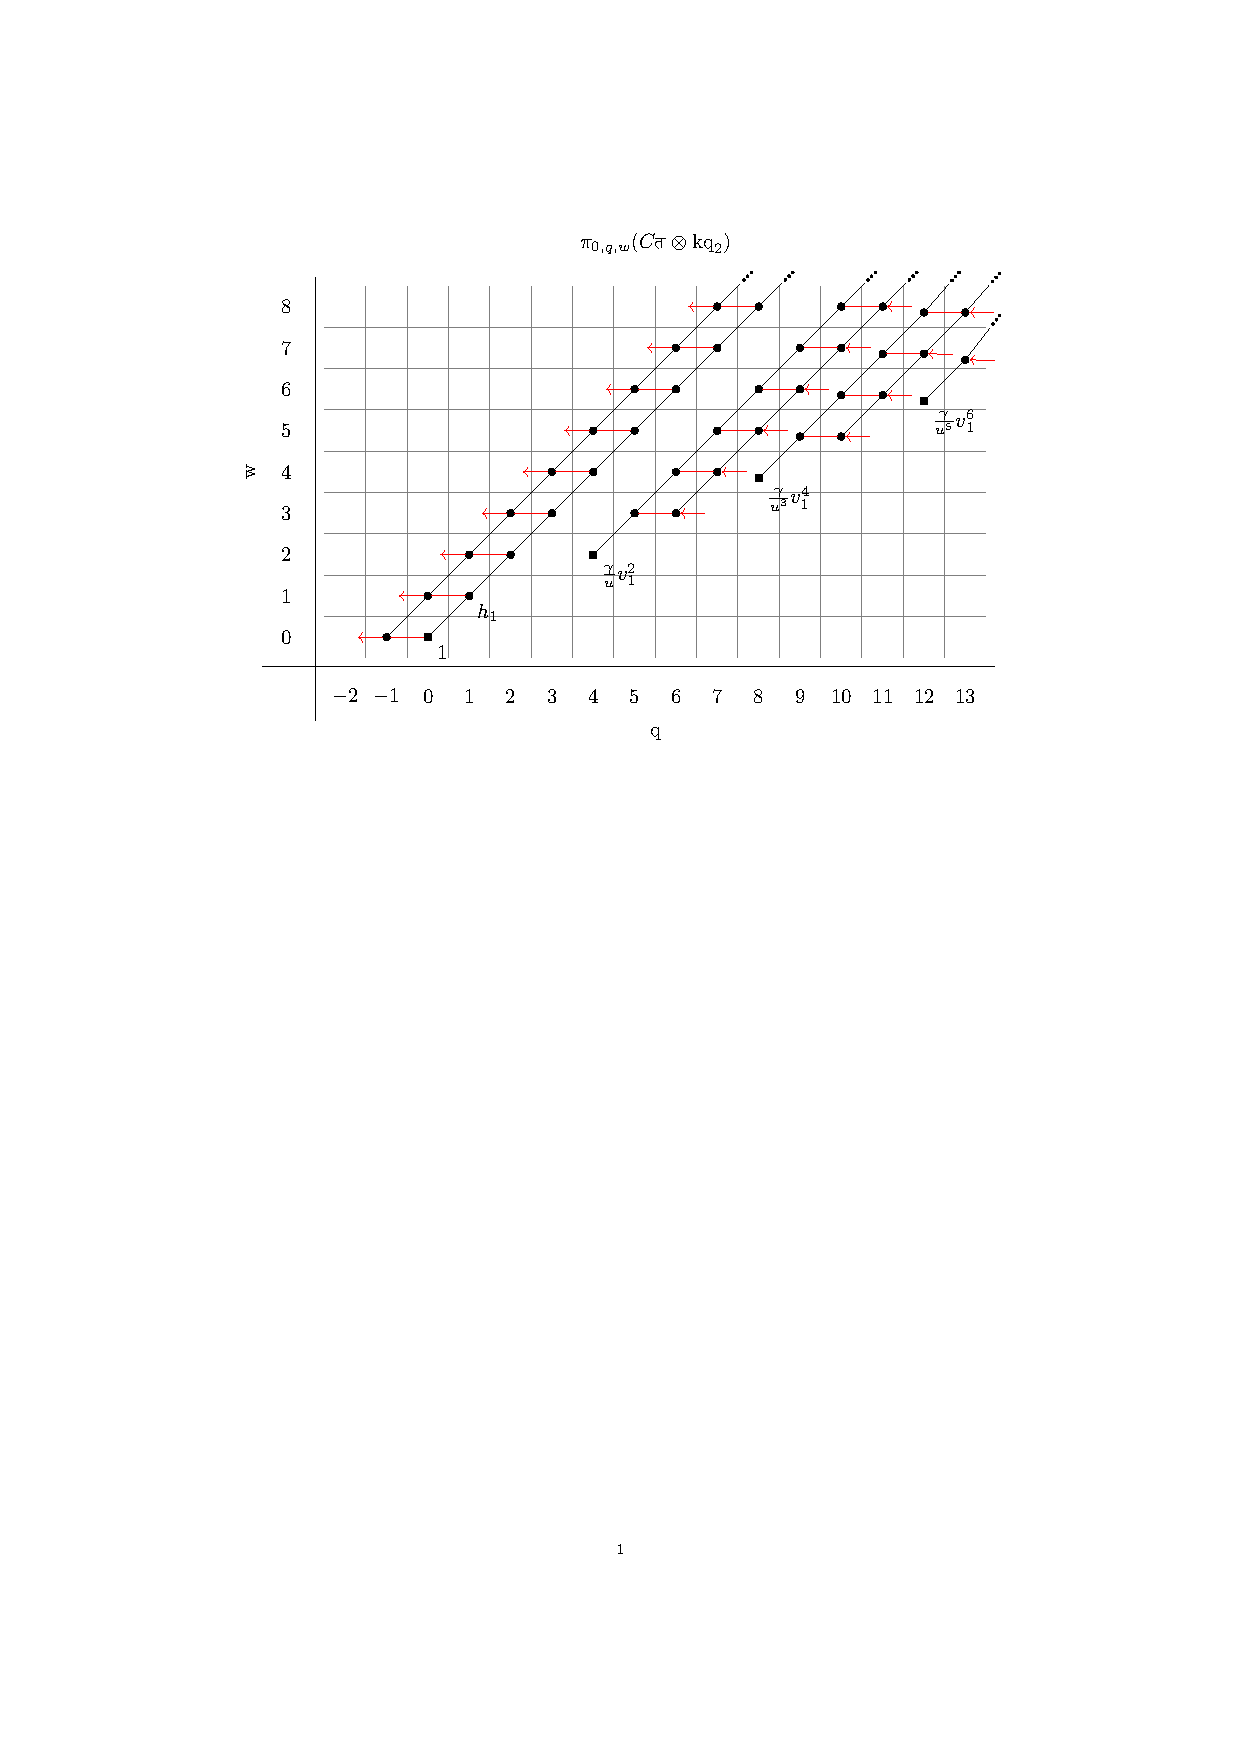
\includegraphics[trim=100 470 100 100, clip, width=\textwidth, scale=0.6]{kqChart1.pdf}
\end{figure}


Red lines denote multiplication by $a \in \pi_{0,-1,0} \Ss$.  Black lines denote multiplication by the motivic $\eta:\mathbb{G}_m \to \Ss$, which in our grading convention lives in $\pi_{0,1,1} \Ss$.

\newpage

\begin{figure}[ht]
\centering
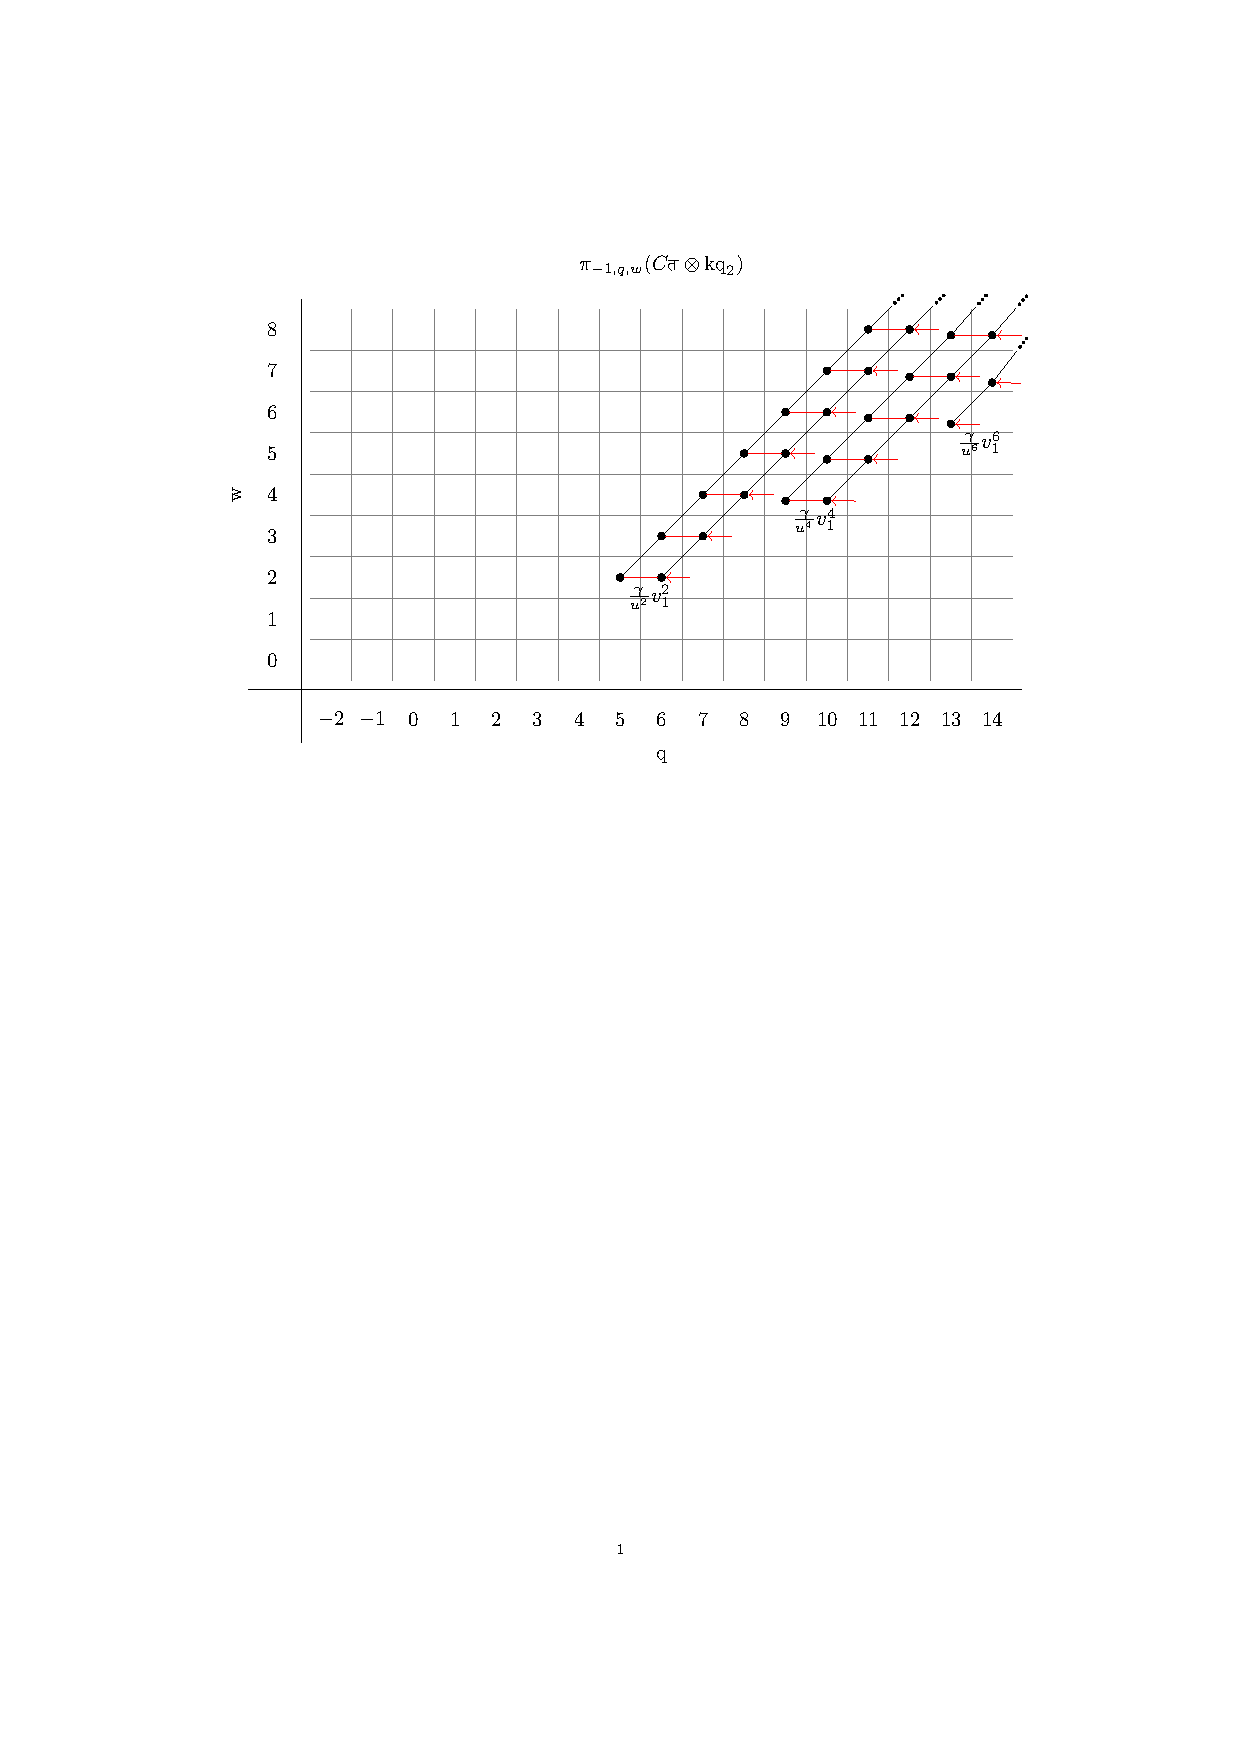
\includegraphics[trim=100 470 100 120, clip, width=\textwidth, scale=0.6]{kqChart2.pdf}
\end{figure}

Below, we depict some of the $\mathrm{E}_{\infty}$-page of the $\ta$-Bockstein spectral sequence for $\pi_{*,*,*} \mathrm{kq}_2$.
We follow the convention introduced in \cite[\S A.2]{Boundaries} and \cite{BurklundExtension} of using blue symbols to denote $\ta$-torsion classes, while black symbols denote $\ta$-torsion free classes.
In particular, black symbols contribute not only to the homotopy group corresponding to the box in which they appear, but also to the groups corresponding to boxes directly below where they appear.
In the language of \cite{Kong}, the blue dots in our charts contain information about which dots on the $\mathrm{E}_1$-page of the $C_2$-effective spectral sequence are targets of differentials, as opposed to sources of differentials.

\begin{figure}[ht]
\centering
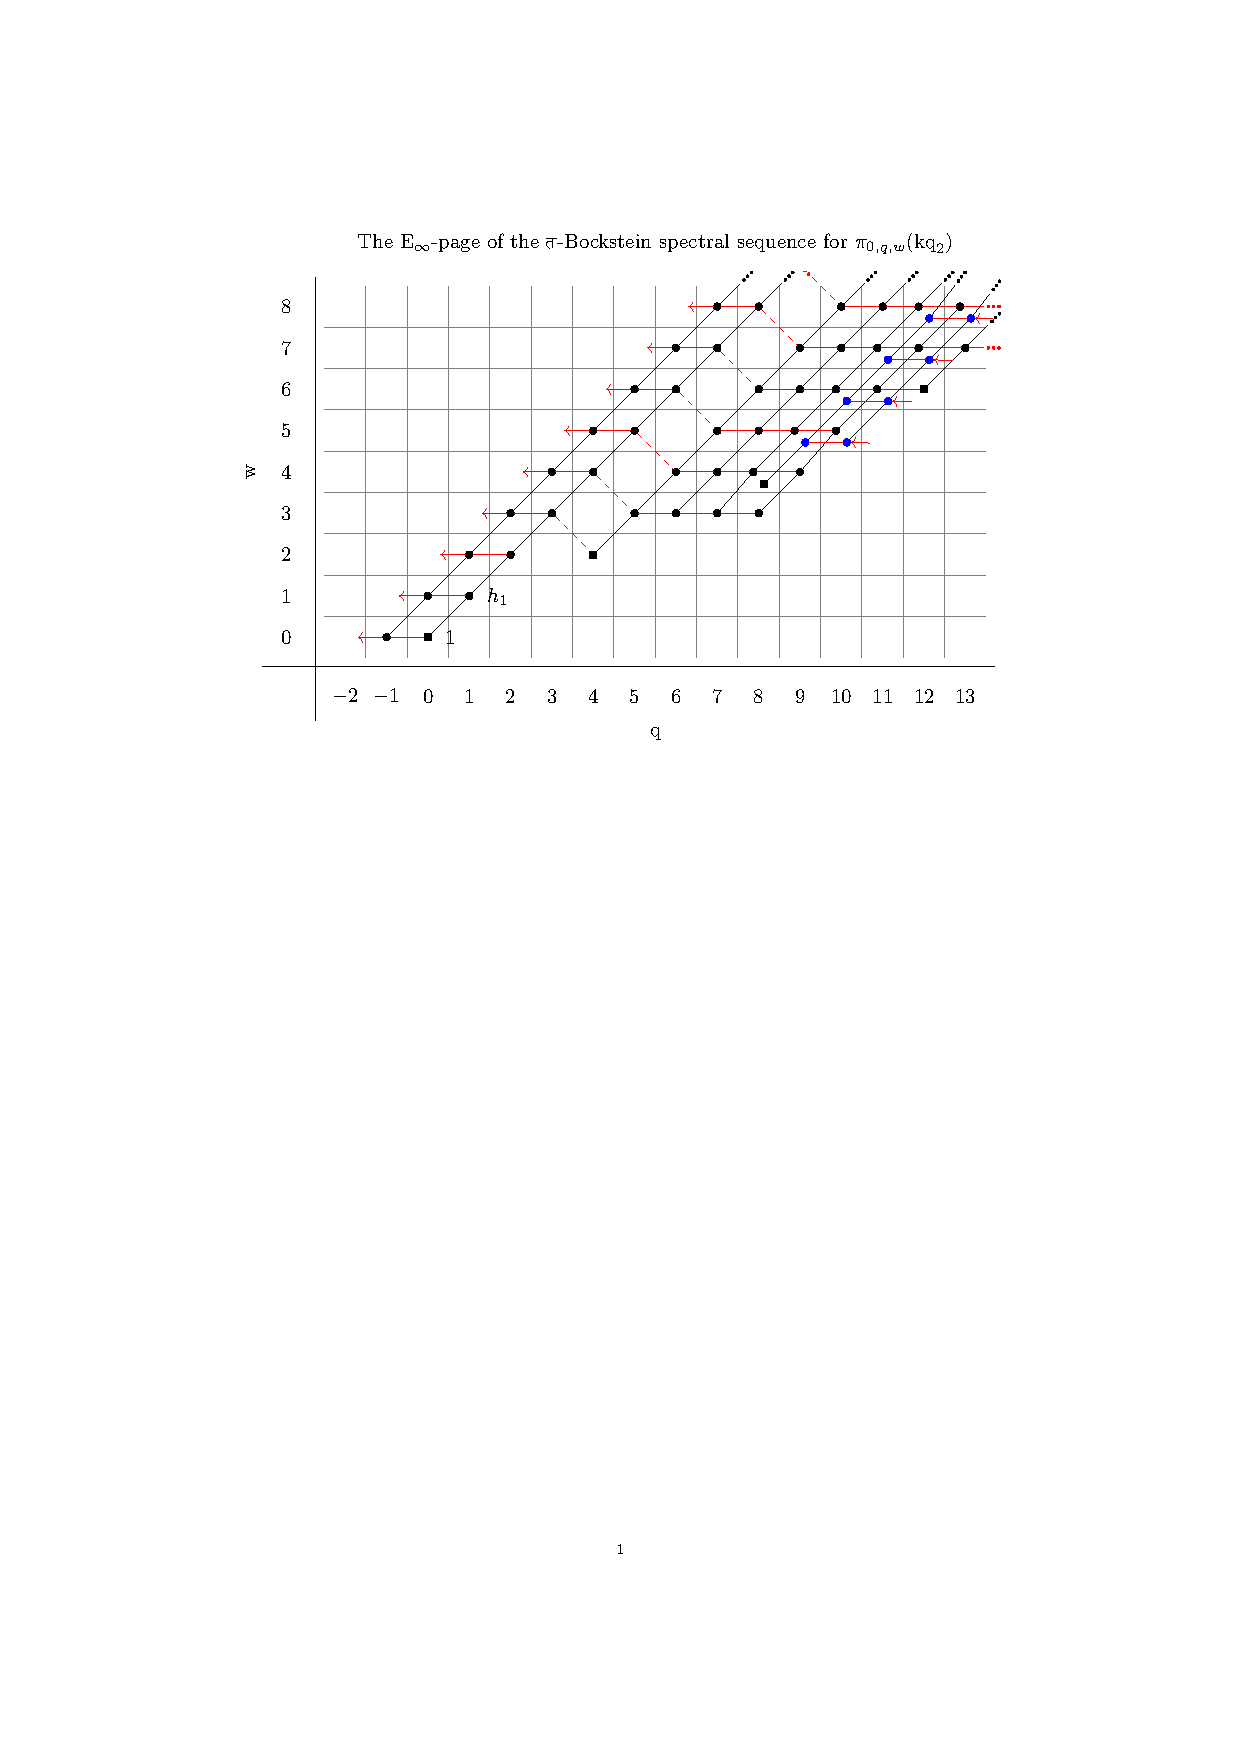
\includegraphics[trim=100 470 100 100, clip, width=\textwidth, scale=0.6]{kqChart3.pdf}
\end{figure}

\begin{figure}[ht]
\centering
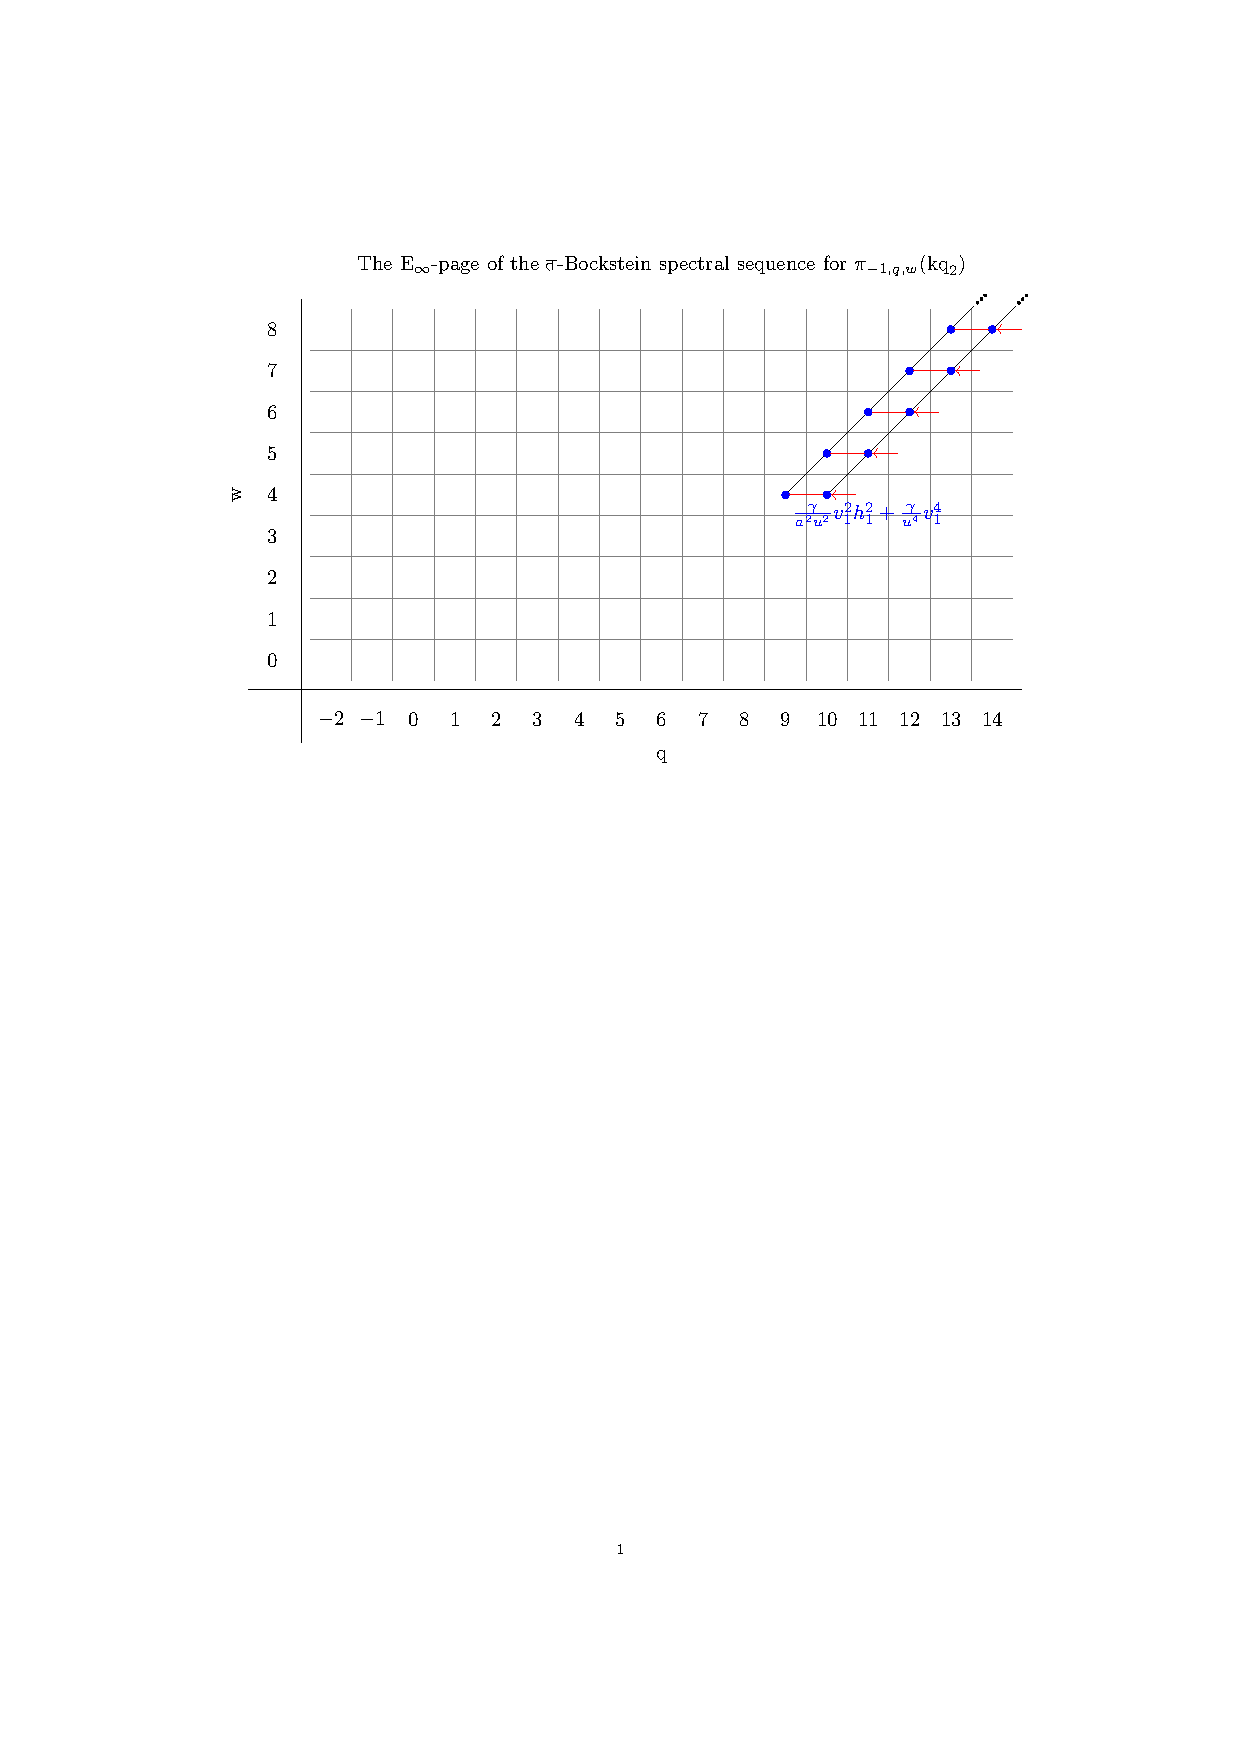
\includegraphics[trim=100 470 100 100, clip, width=\textwidth, scale=0.6]{kqChart4.pdf}
\end{figure}

\begin{rmk}
The groups $\pi_{-1,*,*}\mathrm{kq}_2$ and $\pi_{0,*,*}\mathrm{kq}_2$ assemble, via the multiplication by $a$ long exact sequence, into the homotopy groups $\pi_{0,*,*}\left(Ca \otimes \mathrm{kq}_2\right)$.  These groups in turn record the bigraded homotopy of the $\C$-motivic $\mathrm{kq}_2$.  The reader may note an interesting extension, of the form 
\[2 \mathbb{Z}_2[\tau] \oplus \tau \mathbb{Z}_2[\tau] \to \mathbb{Z}_2[\tau] \to \mathbb{F}_2,\]
which appears when computing $\pi_{0,8,*}(\mathrm{kq}_2^{\wedge} \otimes Ca)$.
This extension is related to the orange dashed line in the final chart of \cite{Kong}.
\end{rmk}




\begin{comment}
In this section, we note that the $\ta$-Bockstein spectral sequence for $\pi_{***} kq^{\wedge}_2$ is an incarnation of the \emph{effective} spectral sequence for $(ko_{C_2})^{\wedge}_2$ studied in CITE.
The trigraded homotopy groups $\pi_{***} kq$ record both the differentials and extension problems present in this spectral sequence.
To give a visual representation of the structure of these homotopy groups, we record the hyperplane $\pi_{4,*,*} kq$ in FIGURE.
This may be directly compared to figure BLAH of CITE, where the integer $4$ is referred to as the `coweight.'

We next indicate how, upon inverting the class $a \in \pi_{0,-1,0} (kq)^{\wedge}_2$, the resulting bigraded homotopy groups record the classical $\Ft$-Adams spectral sequence for $(\Phi^{C_2} ko_{C_2})^{\wedge}_2 \simeq \oplus_{k \ge 0} \Sigma^{4k} \Zt$.
Extension problems in this Adams spectral sequence are invisible to the classical bigraded homotopy groups $\pi_{p,q,q} (kq)^{\wedge}_2$, but are recorded in trigraded homotopy via BLAH.

\begin{rmk}
For a general Galois cellular $X$, we do not expect (?) such a close relationship between the effective spectral sequence and $\ta$-Bockstein spectral sequence.  For example, the $\ta$-Bockstein spectral sequence for the sphere spectrum is more closely related to the Chow--Novikov spectral sequence of CITE.  \todo{justify this... refer to something about Chow--Novikov or something in the sphere or both?}
\end{rmk}

\begin{prop}
There is an additive isomorphism
$\pi_{*,*,*}(kq^{\wedge}_2 \otimes C\ta) \cong \uZt[v_1^2] \oplus \uFt[h_1,v_1^2]{h_1}$,
where $|v_1|=(2,2,2)$ and $|h_1|=(0,1,1)$.
\end{prop}

\begin{proof}
Consider the $2$-completed slice tower converging to $kq^{\wedge}_2$, which as described in CITE has associated graded a direct sum of Eilenberg--MacLane spectra indexed by products of $h_1$ and $v_1^2$.
Since $C\ta$ is a finite complex, we may tensor this tower with $C\ta$ to obtain a tower converging to $kq^{\wedge}_2 \otimes C\ta$.
By CITE, the $E_1$-page of the spectral sequence associated to this tower is $\uZt[v_1^2] \oplus \uFt[h_1,v_1^2]{h_1}$.
No possible differentials or additive extension problems can occur, for tridegree reasons.
\end{proof}

\begin{prop}
The $\ta$-Bockstein spectral sequence
$$\pi_{p,q,w}(kq^{\wedge}_2 \otimes C\ta)[\ta] \implies \pi_{p,q,w}(kq^{\wedge}_2)$$
degenerates at the $\sE_2=\sE_{\infty}$-page.  The $d_1$ differential is determined under the Leibniz rule by the relations
\begin{enumerate}
\item $d_1(u^2)=\ta a^2  u h_1$
\item $d_1(v_1^2)=\ta u h_1^3$
\end{enumerate}
Upon inverting $\ta$, this spectral sequence is identified with the effective spectral sequence for $\pi_{p+q\sigma}((ko_{C_2})^{\wedge}_2)$.
\end{prop}

\begin{proof}
The $d_1$ differential lands in $\ta$-torsion free groups, so its value can be determined after inverting $\ta$.
One then reads off the two claimed $d_1$ differentials from CITE, remembering as always that $\tau=\ta u$ and $\rho = \ta a$. \todo{maybe nicer to directly use the below remark}
To see that these two $d_1$ differentials determine all other $d_1$-differentials via the Liebniz rule, see Remark CITE.

The first page $\ta^{-1} E_1$ of the $\ta$-inverted Bockstein spectral sequence agrees with the first page of the effective spectral sequence studied in CITE, and $\ta^{-1} d_1$ agrees with the $d_1$ differential in the effective spectral sequence CITE.  Kong proves CITE that the effective spectral sequences converges and collapses at $\sE_2=\sE_{\infty}$.  Since the $\ta$-inverted spectral sequence also converges, it must converge to the same groups.  Any additional non-zero differentials in the $\ta$-inverted spectral sequence would make this impossible, and so the $\ta$-inverted spectral sequence must also collapse at $\sE_2$.  Any potential differential in the $\ta$-Bockstein spectral sequence has target a $\ta$-torsion free group, and so would be detected after inverting $\ta$.
\end{proof}

\begin{rmk}
The $d_1$ differentials above can be seen as arising from two independent sources.  The first differential $d_1(u^2) = \ta a^2 u h_1$ arises from a slice differential in $kgl$, and is detected under the natural map $kq \to kgl$.
The second differential $d_1(v_1^2)=\ta u h_1^3$ is detected under the map $kq \to kq \otimes Ca$, and so is essentially $\C$-motivic in origin.
Under the correspondence between cellular $\C$-motivic homotopy and even $MU$-synthetic spectra CITE, one may read this $d_1$-differential off from the $d_3$-differential $d_3(v_1^2)=h_1^3$ in the classical Adams--Novikov spectral sequence for for $\pi_*(ko)$.
\end{rmk}

\begin{cor}
There are differentials
$$d_1(\frac{\theta}{a^i u^j}) = \begin{cases} \frac{\theta}{a^{i-2} u^{j+1}} \ta \text{ if } j=4k+2 \\ 0 \text{ otherwise}. \end{cases}$$
\end{cor}

\begin{proof}
\end{proof}

There are many hidden extensions in the $\ta$-Bockstein spectral sequence.  After inverting $\ta$, these extensions are determined in CITE.  In order to analyze $a^{-1} (kq)_2^{\wedge}$, we will need the following hidden extension:

\begin{prop}
There is a relation
$ a^2 \eta \ta= 2a \ta \in \pi_{***} (kq)^{\wedge}_2$,
which corresponds to a hidden extension
$a^2 h_1 \ta = 2a$
in the $\sE_{\infty}$-page of the $\ta$-Bockstein spectral sequence.
\end{prop}

\begin{proof}
\end{proof}

The following result relates the homotopy groups of $a^{-1} (kq)^{\wedge}_2$ with the classical $\mathbb{F}_2$-Adams spectral sequence for $(\Phi^{C_2} ko_{C_2})^{\wedge}_2 \simeq \oplus_{k \ge 0} \Sigma^{4k} \Zt$.  We use Pstragowski's language of $\Ft$ synthetic spectra to encode this Adams spectral sequence.

\begin{thm}
There is an isomorphism of bigraded rings
$$\pi_{*,0,*} a^{-1} (kq)^{\wedge}_2 \cong \pi_{*,*} \nu_{\Ft}((\Phi^{C_2} ko_{C_2})_2^{\wedge}).$$ \todo{work out how the degrees shear}
Explicitly, this ring is the $\ta$-adic completion of $\mathbb{Z}_2[x,y,\ta]/(\ta x = 2),$
where $|x|=(0,1)$, $|\ta|=(0,-1)$, and $|y|=(4,0)$.
Under the map $(kq)^{\wedge}_2 \to a^{-1} (kq)^{\wedge}_2$, $x$ and $y$ are the images of $a h_1 \in \pi_{0,0,1} (kq)^{\wedge}_2$ and $u^2 v_1^2 \in \pi_{4,0,} (kq)^{\wedge}_2$, respectively.
\end{thm}

\begin{rmk}
There is no $\ta$-torsion in the bigraded homotopy of $a^{-1} (kq)^{\wedge}_2$.  Equivalently, all of the $\ta$-torsion present in the homotopy of $(kq)^{\wedge}_2$ is killed by some power of $a$.  This is a reflection of the fact that the Adams spectral sequence for $(\Phi^{C_2} ko_{C_2})_2^{\wedge}$ degenerates at the $\sE_2$-page, with no higher differentials.
\end{rmk}


CHARTS PUT BELOW WITHOUT CHANGE


We indicate the trigraded homotopy groups $\pi_{p,q,w} (C\ta \otimes kq_2^{\wedge})$ for $p=0$ and $p=-1$.  These may be compared with CITE, where they correspond to the $E_1$-page of the effective spectral sequence in coweights $0$ and $-1$.

\begin{center}
\begin{sseqpage}[ xscale=0.7, yscale=0.7, x range = {-2}{13}, y range = {0}{8}, x tick step = 1, y tick step = 1, class labels = {right}, classes = fill, grid = crossword, x label = {q}, y label = {w}, title = {$\pi_{0,q,w}(C\ta \otimes kq^{\wedge}_2)$}, class labels = {below right = 0.00 em} ]

\class[rectangle, "1"](0,0) 
\class[](-1,0) \structline[red](0,0)
\draw [->,red] (-1,0) -- (-2+0.3,0);

\class["h_1"](1,1)
\class[](0,1) \structline[red]
\draw [->,red] (0,1) -- (-1+0.3,1);

\foreach \i in {2,...,10} { \class(\i, \i) \class(\i-1,\i) \structline[red]  \draw [->,red] (\i-1,\i) -- (\i-2+0.3,\i);}
\foreach \i in {1,...,10} {\structline(\i,\i)(\i-1,\i-1) \structline(\i-1,\i)(\i-2,\i-1)}

\class[rectangle, "\frac{\gamma}{u} v_1^2"](4,2)
\foreach \i in {1,...,10} {
\class(4+\i,2+\i) \structline(3+\i,1+\i)
\class(5+\i,2+\i) \structline[red](4+\i,2+\i)
\draw[->,red](6-0.3+\i,2+\i)--(5+\i,2+\i);
}
\foreach \i in {2,...,9} {
\structline(5+\i,2+\i)(4+\i,1+\i)
}



\class[rectangle, yshift=-0.1, "\frac{\gamma}{u^3} v_1^4"](8,4)
\foreach \i in {1,...,10} {
\class[yshift=-0.1](8+\i,4+\i) \structline(7+\i,3+\i)
\class[yshift=-0.1](9+\i,4+\i) \structline[red](8+\i,4+\i)
\draw[->,red](10-0.3+\i,4+\i-0.15)--(9+\i,4+\i);
}
\foreach \i in {2,...,9} {
\structline(9+\i,4+\i)(8+\i,3+\i)
}


\class[rectangle, yshift=-0.2, "\frac{\gamma}{u^5} v_1^6"](12,6)
\class[yshift=-0.2](13,7) \structline
\class[yshift=-0.2](14,8) \structline
\draw[->,red](13.7,6.7)--(13,7);


\end{sseqpage}
\end{center}





\begin{center}
\begin{sseqpage}[ xscale=0.7, yscale=0.7, x range = {-2}{14}, y range = {0}{8}, x tick step = 1, y tick step = 1, class labels = {right}, classes = fill, grid = crossword, x label = {q}, y label = {w}, title = {$\pi_{-1,q,w}(C\ta \otimes kq^{\wedge}_2)$}, class labels = {below right = 0.00 em} ]

\class["\frac{\gamma}{u^2} v_1^2"](5,2)
\class(6,2) \structline[red]
\draw[->,red](7-0.3,2)--(6,2);

\foreach \i in {1,...,10} {
\class(5+\i,2+\i) \structline(4+\i,1+\i)
\class(6+\i,2+\i) \structline[red](5+\i,2+\i)
\draw[->,red](7-0.3+\i,2+\i)--(6+\i,2+\i);
}
\foreach \i in {1,...,9} {
\structline(6+\i,2+\i)(5+\i,1+\i)
}

\class[yshift=-0.1, "\frac{\gamma}{u^4} v_1^4"](9,4)
\class[yshift=-0.1](10,4) \structline[red]
\draw[->,red](11-0.3,4-0.15)--(10,4);

\foreach \i in {1,...,10} {
\class[yshift=-0.1](9+\i,4+\i) \structline(8+\i,3+\i)
\class[yshift=-0.1](10+\i,4+\i) \structline[red](9+\i,4+\i)
\draw[->,red](11-0.3+\i,4+\i-0.15)--(10+\i,4+\i);
}
\foreach \i in {1,...,9} {
\structline(10+\i,4+\i)(9+\i,3+\i)
}

\class[yshift=-0.2, "\frac{\gamma}{u^6} v_1^6"](13,6)
\draw[->,red](13.7,5.7)--(13,6);
\class[yshift=-0.2](14,7) \structline
\class[yshift=-0.2](15,8) \structline
\draw[->,red](14.7,6.7)--(14,7);

%\class["\frac{\gamma}{u^6} v_1^6"](13,6)

\end{sseqpage}
\end{center}

In these charts, red lines denote multiplication by $a \in \pi_{0,-1,0} \Ss$.  Black lines denote multiplication by the motivic $\eta:\mathbb{G}_m \to \Ss$, which in our grading convention lives in $\pi_{0,1,1} \Ss$.


%% \newpage

Below are charts, for $p=0,-1$, of the $E_{\infty}$-pages of the $\ta$-Bockstein spectral sequence converging to $\pi_{p,q,w} kq_2^{\wedge}$.  The first of these charts may be compared to CITE.

\begin{center}
\begin{sseqpage}[ xscale=0.7, yscale=0.7, x range = {-2}{14}, y range = {0}{8}, x tick step = 1, y tick step = 1, class labels = {right}, classes = fill, grid = crossword, x label = {q}, y label = {w}, title = {$\pi_{-1,q,w}(kq^{\wedge}_2)$}, class labels = {below right = 0.00 em} ]

\class[blue, "\frac{\gamma}{a^2u^2}v_1^2h_1^2 + \frac{\gamma}{u^4}v_1^4"](9,4)
\class[blue](10,4) \structline[red]
\draw[->,red](11-0.3,4)--(10,4);

\foreach \i in {1,...,10} {
\class[blue](9+\i,4+\i) \structline(8+\i,3+\i)
\class[blue](10+\i,4+\i) \structline[red](9+\i,4+\i)
\draw[->,red](11-0.3+\i,4+\i)--(10+\i,4+\i);
}
\foreach \i in {1,...,9} {
\structline(10+\i,4+\i)(9+\i,3+\i)
}

\end{sseqpage}
\end{center}



\begin{center}
\begin{sseqpage}[ xscale=0.7, yscale=0.7, x range = {-2}{13}, y range = {0}{8}, x tick step = 1, y tick step = 1, class labels = {right}, classes = fill, grid = crossword, x label = {q}, y label = {w}, title = {$\pi_{0,q,w}(kq^{\wedge}_2)$} ]

\class[rectangle, "1"](0,0) 
\class[](-1,0) \structline[red](0,0)
\draw [->,red] (-1,0) -- (-2+0.3,0);

\class["h_1"](1,1)
\class[](0,1) \structline[red]
\draw [->,red] (0,1) -- (-1+0.3,1);

\foreach \i in {2,...,10} { \class(\i, \i) \class(\i-1,\i) \structline[red]  \draw [->,red] (\i-1,\i) -- (\i-2+0.3,\i);}
\foreach \i in {1,...,10} {\structline(\i,\i)(\i-1,\i-1) \structline(\i-1,\i)(\i-2,\i-1)}


\class[rectangle](4,2) \structline[red, dashed](4,2)(3,3)
\class(5,3) \structline[red,dashed](4,4) \structline(4,2)
\class(6,3) \structline[red] \class(7,3) \structline[red] \class(8,3) \structline[red]
\class(6,4) \structline[red,dashed](5,5) \structline(5,3) 
\class(7,4) \structline[red] \structline(6,3) 
\class(8,4) \structline[red] \structline(7,3)
\class(9,4) \structline[red] \structline(8,3)
\class(7,5) \structline[red,dashed](6,6) \structline(6,4)
\class(8,5) \structline[red] \structline(7,4)
\class(9,5) \structline[red] \structline(8,4)
\class(10,5) \structline[red] \structline(9,4)
\class(8,6) \structline[red,dashed](7,7) \structline(7,5)
\class(9,6) \structline[red] \structline(8,5)
\class(10,6) \structline[red] \structline(9,5)
\class(11,6) \structline[red] \structline(10,5)
\class[rectangle](12,6) \structline[red]
\class(9,7) \structline[red,dashed](8,8) \structline(8,6)
\class(10,7) \structline[red] \structline(9,6)
\class(11,7) \structline[red] \structline(10,6)
\class(12,7) \structline[red] \structline(11,6)
\class(13,7) \structline[red] \structline(12,6)
\class(14,7) \structline[red]
\class(10,8) \structline[red,dashed](9,9) \structline(9,7)
\class(11,8) \structline[red] \structline(10,7)
\class(12,8) \structline[red] \structline(11,7)
\class(13,8) \structline[red] \structline(12,7)
\class(14,8) \structline[red] \structline(13,7)
\class(11,9) \structline(10,8)
\class(12,9) \structline(11,8)
\class(13,9) \structline(12,8)
\class(14,9) \structline(13,9)

\class[rectangle, yshift=-0.2](8,4) %\structline[orange, dashed](8,3)
\foreach \i in {1,...,10} {
\class[blue, yshift=-0.2](8+\i,4+\i) \structline(7+\i,3+\i,-1)
\class[blue, yshift=-0.2](9+\i,4+\i) \structline[red](8+\i,4+\i,-1)
\draw[->,red](10-0.3+\i,4+\i-0.3)--(9+\i,4+\i,-1);
}
\foreach \i in {2,...,9} {
\structline(9+\i,4+\i,-1)(8+\i,3+\i,-1)
}


\end{sseqpage}
\end{center}


The homotopy groups of $kq_2^{\wedge} \otimes Ca$ record the $\C$-motivic homotopy of $kq_2^{\wedge}$, or in other words the classical Adams--Novikov spectral sequence for $ko^{\wedge}_2$.  Note the extension
$$2 \mathbb{Z}[\tau] \oplus \tau \mathbb{Z}[\tau] \to \mathbb{Z}[\tau] \to \mathbb{F}_2[\tau]/\tau^{2},$$
which appears when computing $\pi_{0,8,*}(kq_2^{\wedge} \otimes Ca)$.
\end{comment}
  
%% \subsection{Comments on the homotopy of $\MGL$}\

%% \todo{This bit needs to be rewritten.}

%% As a corollary of the proof of \Cref{lem:fund-lem}, we can compute the slice spectral sequence for the trigraded homotopy groups of $\MGL$.

%% \begin{cor} \todo{Actually, what happens with the negative cone? Not sure I accounted for that here.}
%%   One may choose a set $x_i \in \pi_{i,i,i} ^\R \MGL$ of generators for the polynomial algebra $\pi_{n,n,n} ^\R \MGL \cong \Zt [x_1, x_2, \dots]$ such that the following is true.
%%   First, the $\mathrm{E}_1$-page of the effective slice spectral sequence for $\MGL$ is of the form $\left(\pi_{a+b\sigma} \uZt \right) [x_1,x_2, \dots]$.
%%   Then, the differentials in the slice spectral sequence are all induced by the Leibniz rule by
%%   \[d_{2^n-1} (u^{2^n}) = a^{2^{n+1}-1} x_{2^n -1} \ta^{2^n-1}.\] \todo{I think this is the right differential length?}
%% \end{cor}

%% \begin{proof}
%%   By the proof of \Cref{lem:fund-lem}, the effective slice spectral sequence for $\pi_{*,*,w} ^{\R} \MGL$ maps isomorphically, up to a regrading, to the slice spectral sequence for $\pi_{*+*\sigma} ^{C_2} P_{2w} \MUR$.
%%   We may therefore deduce the differentials above from the corresponding equivariant slice differentials established in CITE.
%%   It is not hard to use the known computation of the slice spectral sequence for $\MUR$ CITE to deduce that these differentials generate all of the others using the Leibniz rule.
%%   %There are no further differentials because $a$, $\ta$, and the $x_i$ are permament cycles, so at each stage $u^{2^n}$ is the only possible source for a differential.
%% \end{proof}

%% \begin{rmk}
%%   Multiplying the $d_{2^n-1}$ by a factor of $\ta^{2^n}$, we obtain the usual bigraded differentials (CITE):
%%   \[d_{2^n-1} (\tau^{2^n}) = \rho^{2^{n+1}-1} x_{2^n-1}.\]
%% \end{rmk}


%% \subsection{The homotopy of the sphere}\ 

%% \input{charts/chart1.tex}



\appendix

\section{Recollections on compact rigid generation} \label{app:boilerplate}
In this appendix we recall some useful material on compact rigid generation.
Most of this material has appeared elsewhere and all of it is certainly known to experts.
This appendix was mostly included for the convenience of the authors,
though we do hope the reader finds it to be a concise summary of a basic technique in higher algebra.

\begin{dfn}
  A stable, presentably monoidal category $\CC$ is \emph{rigidly generated} if
  it has a family of compact dualizable generators. \footnote{Here and throughout this appendix we only require that an object has a one-sided dual. The side on which an object has a dual will not be important.}
\end{dfn}

Our goal will be to study some properties of monoidal left adjoints out of a rigidly generated category.
This begins with the following construction.

\begin{cnstr}
  Given an $\En$-monoidal left adjoint
  $ f^* : \CC \to \mathcal{D} $,
  its right adjoint $f_*$ is lax $\En$-monoidal.
  In particular, $f_* (\o)$ is an $\En$-ring,
  so we obtain a factorization of $f^*$ as an $\mathbb{E}_{n-1}$-monoidal left adjoint into
  \[ \CC \xrightarrow{ - \otimes f_*\o} \Mod ( \CC ; f_*\o ) \xrightarrow{g^*} \mathcal{D}. \]
  We will say that the adjunction $f$ is \emph{$0$-affine} if $g$ is an adjoint equivalence.
  Note that being $0$-affine is a property of the underlying monoidal functor. \todo{This really should have a cite to Lurie for the functor Mod out of some cartesian fibration.}
\end{cnstr}

The main result of this appendix is a convenient criterion for $f$ to be $0$-affine.
Before we can state that result we make a preparatory definition.

\begin{dfn}
  Given a monoidal left adjoint $f^* : \CC \to \mathcal{D}$,
  we may consider the projection map,
  \[ X \otimes f_*Y \xrightarrow{\eta_f} f_*f^*(X \otimes f_*Y) \simeq f_*(f^*X \otimes f^*f_*Y) \xrightarrow{\epsilon_f} f_*(f^*X \otimes Y). \]
  We will say that $f$ \emph{satisfies the projection formula at $X$},
  if for all $Y$ the projection map is an equivalence.
  If $f$ satisfies the projection formula at $X$ for all $X$, then we say that $f$ \emph{satisfies the projection formula}.
\end{dfn}

\begin{prop} \label{prop:rigid}
  Given a monoidal left adjoint $f^* : \CC \to \mathcal{D}$ between presentable categories, the following statements are true:
  \begin{enumerate}
  \item $f$ satisfies the projection formula for dualizable objects in $\CC$.
  \item If $\CC$ is rigidly generated and $\mathcal{D}$ has compact unit, then $f_*$ preserves colimits.
  \item If $\CC$ is rigidly generated  and $f_*$ preserves colimits, then $f$ satisfies the projection formula.
  \item $f_*$ is conservative if and only if the essential image of $f^*$ contains a family of generators.
  \item If $f$ satisfies the projection formula, $f_*$ preserves colimits and $f_*$ is conservative, then $f$ is $0$-affine.
  \end{enumerate}
\end{prop}

Our arguments follow those from \cite{MNN} fairly closely, though the hypotheses are somewhat different. \todo{Are there more things to cite here?} Before proceeding to the proof of this proposition we give some examples to demonstrate its effectiveness.



\begin{exm} \label{exm:fil-ctau}
In appendix \Cref{app:fil} we study the category $\Sp^{\Fil}$ of filtered spectra, where we denote the shift map $\o(-1) \to \o$ by $\tau$.
  The associated graded functor $\Gr : \Sp^{\Fil} \to \Sp^{\Gr}$ satisfies the conditions of \Cref{prop:rigid}, so we obtain an equivalence of presentably symmetric monoidal categories
  \[ \Sp^{\Gr} \cong \Mod ( \Sp^{\Fil} ; C\tau ). \]
  Here $C\tau$ acquires a commutative algebra structure from the fact that it equivalent to the image of the unit under the right adjoint of $\Gr$.
\end{exm}

\begin{exm} \label{exm:fil-inv-tau}
  Again working with $\Sp^{\Fil}$,
  the realization functor $\Re : \Sp^{\Fil} \to \Sp$ satisfies the conditions of \Cref{prop:rigid}, so we obtain an equivalence of presentably symmetric monoidal categories
  \[ \Sp \cong \Mod ( \Sp^{\Fil} ; \o[\tau^{-1}] ). \]
  Here $\o[\tau^{-1}]$ acquires a commutative algebra structure from the fact that it is equivalent to the image of the unit under $Y$ (the right adjoint of $\Re$).
\end{exm}

\begin{exm}
  Given a finite extension of characteristic zero fields $\ell/k$ we have a symmetric monoidal left adjoint $ i^* : \SH(k) \to \SH(\ell) $.
Using resolution of singularities, Nagata compactification and purity we know that both of these categories are generated by the motives of smooth projective schemes, each of which is dualizable \cite{MotivicModules}. In short,
   both the source and target categories are rigidly generated, with families of compact dualizable generators given by $\Ss^m \otimes (\P^1)^{\otimes n} \otimes X$ where $X$ is a smooth projective scheme over the base.
  
  In order to show that $i$ is 0-affine we only need to show that the image of $i^*$ contains a family of generators. Given a smooth projective $\ell$-scheme $X$ the projection formula \Cref{prop:rigid}(1) gives us an equivalence
  \[ i_*(\Ss^m \otimes (\P^1)^{\otimes n} \otimes X) \simeq \Ss^m \otimes (\P^1)^{\otimes n} \otimes i_*X. \]
  Since for field extensions $i_{\sharp} = i_*$, we learn that $i_*X = X$ where the second copy of $X$ is considered as a $k$-scheme. It will now suffice to show that $X$ is a retract of $i^*i_*X$. At the level of schemes this means looking at $ X \times_{\Spec(\ell)} \Spec(\ell) \times_{\Spec(k)} \Spec(\ell) $. Using the maps $\ell \to \ell \otimes_k \ell \to \ell$ we may conclude.

  Stated more explicitly,
  we have an equivalence of presentably symmetric monoidal categories
  \[ \SH(\ell) \cong \Mod( \SHk ; \Spec(\ell) ). \]
  Using the fact that $i$ restricts to the subcategories of Artin--Tate objects the same argument provides an equivalence of presentably symmetric monoidal categories
  \[ \SH(\ell)^{\at} \cong \Mod ( \SHkat ; \Spec(\ell) ). \]
\end{exm}

\begin{exm} \label{exm:c2-underlying}
  The category of $C_2$-spectra is rigidly generated and the underlying spectrum functor, $\Phi^e$, is essentially surjective.  We may thus apply \Cref{prop:rigid} to obtain a symmetric monoidal equivalence
  \[ \Mod( \Sp_{C_2} ; R_1) \simeq \Sp, \]
  where $R_1$ is the image of $\Ss$ under the right adjoint to $\Phi^e$.
  Since $\Phi^e$ can be described as homotopy fixed points (or homotopy orbits) composed with $(C_{2})_+ \otimes -$, we find that its right adjoint is given by tensoring with $(C_{2})_+ \simeq Ca_\sigma$. Therefore, $R_1 \simeq Ca_\sigma$.

  Similarly, with $\Phi^e$ replaced by $\Phi^{C_2}$ we obtain a symmetric monoidal equivalence
  \[ \Mod( \Sp_{C_2} ; R_2) \simeq \Sp, \]
  where $R_2$ is the image of $\Ss$ under the right adjoint to geometric fixed points.
  We can compute that $R_2 \simeq \Ss[a_\sigma^{-1}]$ using the presentation of $C_2$-spectra via an isotropy separation square. 
\end{exm}

\begin{exm} \label{exm:c2-graded}
  Taking loops on the map $i : S^1 \to B\Pic(\Sp_{C_2})$ which sends a generator to $\Ss^{\sigma}$ we get a monoidal functor $i : \Z \to \Pic(\Sp_{C_2})$. Embedding the target into $\Sp_{C_2}$ and tensoring up to spectra we obtain a monoidal left adjoint,
  \[ i^* : \Sp^{\Gr} \to \Sp_{C_2} \]
  which sends $\Ss(1)$ to $\Ss^{\sigma}$. Since $\Sp^{\Gr}$ is rigidly generated, the unit in $\Sp_{C_2}$ is compact and the representation spheres generate $\Sp_{C_2}$ we may apply \Cref{prop:rigid} to conclude that $i$ is $0$-affine. Stated more explicitly,
  we have an equivalence of presentable categories,
  \[ \Sp_{C_2} \cong \Mod( \Sp^{\Gr} ; i_*\Ss ). \]
  The graded ring $i_*\Ss$ has $n^{\mathrm{th}}$ term given by $\Map^{\Sp} ( \Ss^{n\sigma}, \Ss )$.
  Expressed in terms of stunted projective spaces we have $(i_*\Ss)_n \simeq \Sigma \R \mathrm{P}_{-\infty}^{-n-1}$. %The authors will return to the question of whether this example can be upgraded to an $\mathbb{E}_1$-deformation of spectra in the sense of the \Cref{app:def} in the future. 
\end{exm}


\begin{proof}[Proof (of \Cref{prop:rigid}(1)).]    
  Consider the following commutative diagram, which is natural in $X \in \CC^{\mathrm{dbl}}$, $Y \in \mathcal{D}$ and $Z \in \mathcal{C}$. 
  {\footnotesize
    \begin{center} \begin{tikzcd}
        \Map_{\mathcal{C}}(X^\vee \otimes Z, f_*Y) \ar[r] \ar[rr, "\simeq", bend left=10] &
        \Map_{\mathcal{D}}(f^*(X^\vee \otimes Z), f^*f_*Y) \ar[d, "\simeq"] \ar[r] &
        \Map_{\mathcal{D}}(f^*(X^\vee \otimes Z), Y) \ar[d, "\simeq"] \\        
        & \Map_{\mathcal{D}}(f^*(X^\vee) \otimes f^*Z, f^*f_*Y) \ar[d, "\simeq"] \ar[r] &
        \Map_{\mathcal{D}}(f^*(X^\vee) \otimes f^*Z, Y) \ar[d, "\simeq"] \\
        \Map_{\mathcal{C}}(Z, X \otimes f_*Y) \ar[d] \ar[uu, no head, "\simeq"] &
        \Map_{\mathcal{D}}((f^*X)^\vee \otimes f^*Z, f^*f_*Y) \ar[d, "\simeq"] \ar[r] &
        \Map_{\mathcal{D}}((f^*X)^\vee \otimes f^*Z, Y) \ar[d, "\simeq"] \\
        \Map_{\mathcal{D}}(f^*Z, f^*(X \otimes f_*Y)) \ar[r, "\simeq"] &
        \Map_{\mathcal{D}}(f^*Z , f^*X \otimes f^*f_*Y) \ar[r] &
        \Map_{\mathcal{D}}(f^*Z , f^*X \otimes Y) 
    \end{tikzcd} \end{center}
  }
  The rectangle on the left commutes due to the compatibility of dualization with the monoidal structure on $f^*$. The remaining squares commute for easier reasons. Now observe that starting in the middle of the left side and proceeding counter-clockwise gives the projection map, while proceeding clockwise given an equivalence.
\end{proof}

\begin{proof}[Proof (of \Cref{prop:rigid}(2)).]
  Since $\CC$ is rigidly generated it has a family of compact dualizable generators.
  Monoidal functors send dualizable objects to dualizable objects.
  Since the unit of $\mathcal{D}$ is compact we learn that $f^*$ sends dualizable objects to compact objects.
  Thus, since $f^*$ sends a family of compact generators to compact objects its right adjoint $f_*$ preserves colimits.
\end{proof}

\begin{proof}[Proof (of \Cref{prop:rigid}(3)).]
  The projection formula asks that the natural projection map
  \[ X \otimes f_*Y \to f_*(f^*X \otimes Y) \]
  be an equivalence.
  Using the hypotheses that $f_*$ preserves colimits and $\CC$ is rigidly generated we can reduce to the case where $X$ is a compact dualizable generator. 
  We may now use \Cref{prop:rigid}(1) to conclude.
\end{proof}

\begin{proof}[Proof (of \Cref{prop:rigid}(4)).]
  Clear.
\end{proof}

\begin{proof}[Proof (of \Cref{prop:rigid}(5)).]
  We begin by showing that $g^*$ is fully faithful.
  This is equivalent to showing that the unit map
  $X \to g_*g^*X$ is an equivalence.
  Applying the projection formula with $Y = \o$, we can conclude that this is true for induced $f_*\o$-modules.
  Since $f_*$ preserves colimits and $\Mod( \CC ; f_*\o)$ is generated by induced $f_*\o$-modules this is sufficient to conclude.

  Now, we show that $g^*$ is essentially surjective.
  By \Cref{prop:rigid}(4) we know the essential image of $f^*$ contains a family of generators (and $g^*$ has the same property).
  Using fully-faithfulness we can now conclude that $g^*$ is essentially surjective.  
\end{proof}

We close the appendix with another useful lemma.

\begin{lem} \label{lem:tensor-mod}
  Suppose that $\CC$ and $\D$ are stable presentably symmetric monoidal categories, and let $R$ be a commutative algebra in $\CC$.
  Given a symmetric monoidal left adjoint $f^* : \CC \to \mathcal{D}$, 
  there is an equivalence of presentably symmetric monoidal categories
  \[\Mod(\D; f^*R) \simeq \Mod(\CC; R) \otimes_\CC \D.\]
\end{lem}

\begin{proof}
  This follows from \cite[Theorem 4.8.5.16]{HA} after unraveling the definitions.
\end{proof}

\begin{exm}  
  Given a stable presentably symmetric monoidal category $\CC$ and a commutative algebra $R \in \CC^{\Fil}$, this lemma provides an equivalence
  \[ \Sp^{\Gr} \otimes_{\Sp^{\Fil}} \Mod ( \CC^{\Fil} ; R ) \simeq \CC^{\Gr} \otimes_{\CC^{\Fil}} \Mod ( \CC^{\Fil} ; R ) \simeq \Mod ( \CC^{\Gr} ; \Gr(R) ) \]
\end{exm}


\section{Recollections on filtered objects} \label{app:fil}
%% \subsubsection{Recollections on filtered objects}

%% Before we describe our deformation machine, we first recall some basic properties of the categories of filtered and graded objects in a category $\CC$.

In this appendix we give a more detailed introduction to filtered objects.
The results here are well-known (cf. \cite{RotationInvariance}), and we aim mainly to fix notation.

\begin{cnv}
  In this appendix, $\CC$ will denote a stable, presentable category.
  %% When we ask for $\CC$ to be $\En$-monoidal, we will always assume that it is presentably $\En$-monoidal, i.e. that the tensor product preserves colimits in each variable separately.
  We will use $\o$ to denote the unit of $\CC$ when it is monoidal.
\end{cnv}


\begin{dfn}
  We let $\Z$ denote the symmetric monoidal category with underlying category given by the discrete set $\Z$ and symmetric monoidal structure given by addition.

  Similarly, we let $\Z^{\Fil}$ denote the symmetric monoidal category with underlying category given by the poset $\Z$ with its order $\leq$, so that there is a unique map $n \to m$ whenever $n \leq m$, and symmetric monoidal structure given by addition.
\end{dfn}

\begin{dfn}
  Given a category $\CC$, we let $\CC^{\Fil} \coloneqq \Fun(\Z^{\Fil,op}, \CC)$ denote the category of filtered objects in $\CC$.
  Objects of $\CC^{\Fil}$ are diagrams
  \[ \dots \to C_2 \to C_1 \to C_0 \to C_{-1} \to C_{-2} \to \dots \]
  in the category $\CC$. We will sometimes use the notation $C_\bullet$ for an object of $\CC^{\Fil}$.
  \begin{itemize}
  \item There is a natural left adjoint $c : \CC \to \CC^{\Fil}$, which sends $C$ to the constant object
    \[ \dots \to 0 \to 0 \to C \xrightarrow{\id} C \xrightarrow{\id} C \xrightarrow{\id} \dots \]
    that is equal to $C$ in nonpositive degrees and $0$ in positive degrees.
  \item There is a natural left adjoint $Y : \CC \to \CC^{\Fil}$, which sends $C$ to the constant object
    \[ \dots \xrightarrow{\id} C \xrightarrow{\id} C \xrightarrow{\id}  C \xrightarrow{\id} C \xrightarrow{\id} C \xrightarrow{\id} \dots \]
    that is equal to $C$ in each degree.
  \item The functor $Y$ admits a left adjoint $\Re : \CC^{\Fil} \to \CC$, which sends
    $C_\bullet$ to $\varinjlim_{n} C_{-n}$.
  \item The category $\CC^{\Fil}$ admits natural automorphisms $(k) : \CC^{\Fil} \to \CC^{\Fil}$ that send $C_\bullet$ to $C_{\bullet - k}$.
  \item There is a natural transformation $\tau : (-1) \to \mathrm{Id}$, which captures the shift map in the filtration. We depict $\tau$ on $cX$ below,
  \begin{center}
    \begin{tikzcd}
      \dots \ar[r] & 0 \ar[r] \ar[d] & 0 \ar[r] \ar[d] & 0 \ar[r] \ar[d] & X \ar[r] \ar[d] & X \ar[d] \ar[r] & \dots \\
      \dots \ar[r] & 0 \ar[r] & 0 \ar[r] & X \ar[r] & X \ar[r] & X \ar[r] & \dots
    \end{tikzcd}
  \end{center}
  If $\CC$ is monoidal, then we will refer to the cofiber of $\tau : \o(-1) \to \o$ as $C\tau$.
  \end{itemize}

  We let $\CC^{\Gr} \coloneqq \Fun(\Z^{op}, \CC)$ denote the category of graded objects in $\CC$.
  Objects of $\CC^{\Gr}$ are collections $\{C_n\}_n$ of objects of $\CC$.
  We will sometimes use the notation $C_*$ for an object of $\CC^{\Gr}$.
  \begin{itemize}
  \item There is a natural fully-faithful left adjoint $c : \CC \to \CC^{\Gr}$, which sends $C$ to $C_*$ with $C_0 = C$ and $C_k = 0$ for $k \neq 0$.
  \item There is a natural left adjoint $\Gr : \CC^{\Fil} \to \CC^{\Gr}$, which sends
  \[ \dots \to C_2 \to C_1 \to C_0 \to C_{-1} \to C_{-2} \to \dots \]
  to $\{C_n / C_{n+1}\}_n$.
  \end{itemize}
  
  If $\CC$ is a presentably $\mathbb{E}_{n}$-monoidal category,
  then $\CC^{\Fil}$ and $\CC^{\Gr}$ inherit the structure of $\En$-monoidal categories under Day convolution,
  and the functors $c$, $Y$, $\Re$, $c$ and $\Gr$ are all $\En$-monoidal.
\end{dfn}

\begin{rmk}
  Using the assumption that $\CC$ is stable and presentable we can offer another description of the categories of filtered and graded objects, which is often useful in proofs.
  \[ \CC^{\Fil} \simeq \Sp^{\Fil} \otimes\ \CC \quad \text{ and } \quad \CC^{\Gr} \simeq \Sp^{\Gr} \otimes\ \CC. \]
  Since it is well-known that the analogs of $c$, $Y$, $\Re$, $c$ and $\Gr$ are symmetric monoidal in the case of spectra, the claims about $\En$ monoidality made above follow by tensoring up. 
\end{rmk}

Using the fact that $\o(1) \otimes \o(-1) \simeq \o$, we learn that if $X$ is a dualizable object of $\CC$, then $c(X)(n)$ is a dualizable object of $\CC^{\Fil}$. Similarly, we have that if $\{X_\alpha\}$ is a set of compact (dualizable) generators of $\CC$, then $\{c(X_\alpha)(k)\}$ is a set of compact (dualizable) generators of $\CC^{\Fil}$.

%% \begin{cnstr} \label{cnstr:twist}
%%   Suppose that $\CC$ is an $\En$-monoidal category.
%%   We let $\o (k) \in \CC$ denote the object which is equal to $\o$ in degrees $\leq k$ and $0$ in degrees $> k$, and all of whose maps are either $0$ or $\id_{\o}$.
%%   Then $\o(0)$ is the unit of $\CC^{\Fil}$ and $\o(k) \otimes \o(\ell) \simeq \o(k+\ell)$.
%%   Given $C \in \CC$ and $k \in \Z$, we let $C(k) \coloneqq c(C) \otimes \o(k)$.
%%   Then, for each $k$, $C \mapsto C(k)$ is a colimit-preserving functor, and the joint image of these functors generate $\CC^{\Fil}$ under colimits.

%%   We let $\tau : \o(1) \to \o$ denote the map
%%   \begin{center}
%%     \begin{tikzcd}
%%       \dots \ar[r] & 0 \ar[r] \ar[d] & 0 \ar[r] \ar[d] & 0 \ar[r] \ar[d] & \o \ar[r] \ar[d] & \o \ar[d] \ar[r] & \dots \\
%%       \dots \ar[r] & 0 \ar[r] & 0 \ar[r] & \o \ar[r] & \o \ar[r] & \o \ar[r] & \dots
%%     \end{tikzcd}
%%   \end{center}
%%   where all the maps between $\o$ are the identity.

%%   Then the cofiber of $\tau$, $C\tau$, is of the form
%%   \[ \dots \to 0 \to 0 \to \o \to 0 \to 0 \to \dots,\]
%%   and is easily seen to admit a canonical $\mathbb{E}_{n}$-ring structure.

%%   Similarly, $\o[\tau^{-1}]$ admits a canonical $\mathbb{E}_{n}$-ring structure and is of the form
%%   \[ \dots \to \o \xrightarrow{\id_\o} \o \xrightarrow{\id_\o} \o \xrightarrow{\id_\o} \o \xrightarrow{\id_\o} \o\to \dots. \]
%% \end{cnstr}

%% AAAAAAAAAAAAAAAAAAAAAAAAAAAAAAAAAAAAAAAAAAAAAAAaaa

\begin{lem} \label{prop:mod-fil}
  Given an $\En$-monoidal category $\CC$,
  the image of $\o$ under the right adjoint of $\Re$ is $\o[\tau^{-1}]$;
  therefore this object is an $\En$-algebra and there is an equivalence of $\mathbb{E}_{n-1}$-monoidal categories
  $ \Mod(\CC^{\Fil}; \o[\tau^{-1}]) \simeq \CC $.
  Similarly,
  the image of $\o \in \CC^{\Gr}$ under the right adjoint of $\Gr$ is $C\tau$;
  therefore this object is an $\En$-algebra and there is an equivalence of $\mathbb{E}_{n-1}$-monoidal categories
  $ \Mod(\CC^{\Fil}; C\tau) \simeq \CC^{\Gr}. $
  Moreover, the functors $- \otimes \o[\tau^{-1}]$ and $- \otimes C\tau$ are identified under these equivalences with $\Re$ and $\Gr$, respectively.
\end{lem}

\begin{proof}
  The case of spectra was handled in Examples \ref{exm:fil-ctau} and \ref{exm:fil-inv-tau}.
  For a general $\CC$ we just tensor the case of spectra with $\CC$.
\end{proof}


\section{A machine for deforming homotopy theories} \label{app:def}
In this appendix, we have two goals.
The first is to identify a technique which produces 1-parameter deformations in homotopy theory.
This technique is essentially an elaboration of \cite[Definition 3.2]{cmmf}.
The second goal is to provide a recognition criterion for 1-parameter deformations.
This criterion will be applied in \Cref{sec:top} of the main paper to identify $\SHRat$ with the category of modules over a commutative algebra in $i2$-complete filtered $C_2$-spectra.

The approach to deforming categories taken here is different than the approach taken in Pstr\k{a}gowski's theory of synthetic spectra \cite{Pstragowski}, which is a theory specifically about deformations of $\Sp$. %Notably, the input to define a category of synthetic spectra is much less rigid.On the other hand, when both are defined we will show that they agree for the most part. This in turn suggests that a far more general version of Pstr\k{a}gowski's approach is possible, where an arbitrary (symmetric monoidal) presentable category is deformed. 
When our construction here and Pstr\k{a}gowki's construction are both defined, we will show that they are equivalent up to a minor completion issue. This in turn suggests that a more general version of Pstr\k{a}gowski's approach is possible, where an arbitrary (symmetric monoidal) presentable category is deformed. 

This appendix is not intended to be a definitive treatment of deformations.  Instead, we view at as an illustration of a variety of elementary techniques, which in combination produce a large collection of interesting examples.
%Instead it is supposed to be an illustration of how combining couple elementary techniques in a clever way can produce a large collection of interesting examples.

\subsection{Constructing deformations} \label{app:def-const}\

In this section we will give techniques for producing 1-parameter deformations.

\begin{cnv}
  In this section, $\CC$ will denote a stable presentably symmetric monoidal category.
  %% When we ask for $\CC$ to be $\En$-monoidal, we will always assume that it is presentably $\En$-monoidal, i.e. that the tensor product preserves colimits in each variable separately.
  We will use $\o$ to denote the unit of $\CC$, and assume the notation of \Cref{app:fil} %% when it is $\En$-monoidal.
\end{cnv}

The deformations we produce will all be of the form
\[ \Mod ( \CC^{\Fil} ; R ) \]
for some kind of algebra $R$.\footnote{Although much of the material in this appendix applies for $\En$-algebras in $\En$-monoidal categories, the extra generality was not necessary for this work.}
Therefore, what we really do is give methods for constructing algebras in filtered objects.



We will produce commutative algebras in $\CC^{\Fil}$ through the following method.
Given a lax symmetric monoidal functor $F : \CC \to \CC^{\Fil}$, the image of the unit $F(\o)$ is a commutative algebra in $\CC^{\Fil}$. If we let $L$ denote the composite $\Re \circ F$, then we have the following proposition.

\begin{prop}
  The presentably symmetric monoidal category $\Mod(\CC^{\Fil}; F(\o))$ is a 1-parameter deformation in the sense that,
  \begin{enumerate}
  \item There is a colimit-preserving symmetric monoidal functor out of $\CC^{\Fil}$ with target $\Mod(\CC^{\Fil}; F(\o))$.
  \item The generic fiber is given by $\Mod(\CC; L(\o))$, in the sense that
    there is an equivalences of presentably symmetric monoidal categories
    \[\Mod(\CC^{\Fil}; F(\o)[\tau^{-1}]) \simeq \Mod(\CC; L(\o)). \]
  \item The special fiber is given by $\Mod(\CC^{\Gr}; \Gr F(\o) )$, in the sense that
    there is an equivalences of presentably symmetric monoidal categories
    \[\Mod(\CC^{\Fil}; F(\o) \otimes C\tau) \simeq \Mod(\CC^{\Gr}; \Gr(F(\o))).\]
  \end{enumerate}
  Moreover, when viewed as a lax symmetric monoidal functor, $F$ factors as
  \[ \CC \xrightarrow{G} \Mod(\CC^{\Fil}; F(\o)) \to \CC^{\Fil}. \]
\end{prop}

\begin{proof}
  This follows immediately from \Cref{prop:mod-fil} and \Cref{lem:tensor-mod}. \todo{update when this breaks.}
\end{proof}

We will refer to lax symmetric monoidal functors $T : \CC \to \CC^{\Fil}$ as \emph{tower functors} and give several examples.

\begin{exm}
  The functors $c$ and $Y$ are tower functors.
\end{exm}

\begin{exm}
  The functor $\tau_{\geq \bullet} : \Sp \to \Sp^{\Fil}$ is a tower functor.
\end{exm}

\begin{exm}
  If $\CC$ has a $t$-structure which is compatible with the tensor product in the sense that the unit is connective and the tensor product of two connective objects is connective, then
  \[ \tau_{\geq \bullet} : \CC \to \CC^{\Fil} \]
  is a tower functor. More generally we have a tower functor
  $ \tau_{\geq m \bullet} : \CC \to \CC^{\Fil} $ for natural numbers $m$.
\end{exm}

\begin{cnstr} \label{cnstr:trunc-tower}
  Suppose we are given a collection $A$ of coreflective subcategories $\CC^A_{\geq k} \subset \CC$,
  such that
  \begin{itemize}
  \item if $X \in \CC^A_{\geq k}$ and $Y \in \CC^A_{\geq \ell}$, then $X \otimes Y \in \CC^A_{\geq k+\ell}$.
  \item $\CC^A_{\geq k+1} \subset \CC^A_{\geq k}$ and $\o \in \CC^A_{\geq 0}$.
  \end{itemize}

  Let $\tau_{\geq k} : \CC \to \CC^A_{\geq k}$ denote the right adjoints of the inclusions. 
  Then, we can assemble these categories into a single coreflective subcategory $\CC_{\geq 0}^{\Fil, A}$
  consisting of filtered objects
  \[\dots \to X_2 \to X_1 \to X_0 \to X_{-1} \to X_{-2} \to \dots\]
  for which $X_i \in \CC^A_{\geq i}$.
  %% Since the $\CC_{\geq \bullet} \subset \CC$ are coreflective subcategories, it is easy to see that $\CC^{\Fil}_{\geq 0} \subset \CC^{\Fil}$ is coreflective as well.
  The right adjoint $\tau_{\geq 0}^A : \CC^{\Fil} \to \CC^{\Fil, A}_{\geq 0}$ to the inclusion is given by applying $\tau_{\geq i}$ in position $i$.
  %% \[\dots \to C_2 \to C_1 \to C_0 \to C_{-1} \to C_{-2} \to \dots\]
  %% to
  %% \[\dots \to \tau_{\geq 2} C_2 \to \tau_{\geq 1} C_1 \to \tau_{\geq 0} C_0 \to \tau_{\geq -1} C_{-1} \to \tau_{\geq -2} C_{-2} \to \dots.\]

  Our assumptions guarantee that $\CC_{\geq 0}^{\Fil, A}$ is closed under the tensor product and so admits a natural presentably symmetric monoidal structure, for which the inclusion $\CC^{\Fil, A}_{\geq 0} \subset \CC^{\Fil}$ is a symmetric monoidal functor. As a consequence, we obtain a lax symmetric monoidal endofunctor  
   \[ \tau^A_{\geq 0} : \CC^{\Fil} \to \CC^{\Fil}. \]
\end{cnstr}

\begin{exm}
  If $\CC$ is the category of $G$-equivariant spectra for some finite group $G$, then we can let $\CC^{\mathrm{slice}}_{\geq k}$ be the regular slice $k$-connective $G$-spectra.\footnote{Note that we cannot use the classical slice filtration here, unless $m$ is divisible by $\abs{G}$ in which case it agrees with the regular one, since it is not compatible with the tensor product.} As a variant we could also take the regular slice $mk$-connective subcategories for some positive integer $m$.
\end{exm}

Each of the above examples of tower functors can be described as a composite of $Y$ with an appropriately chosen $\tau_{\geq 0}$.
This construction can be considered a generalization of the twisted $t$-structures on filtered objects considered in \Cref{subsec:twists}.
Thus, so far we have only produced ``truncation type towers.''
We now give a construction which takes in a tower functor $T$ and a commutative algebra in $\CC$ and produces a new tower functor. This construction will have the effect of shearing the Adams spectral sequence based on $E$ along the tower $T$. To begin, we review the monoidal properties of the cobar construction.

\begin{cnstr}
  Since the coproduct of commutative algebras in $\CC$ is given by the tensor product, % on underlying.
  the cobar construction can be upgraded into a functor
  \[ \mathrm{cb} : \CAlg (\CC) \to \CAlg (\CC^{\Delta}) .\]
  %% Given a presentably symmetric monoidal categeory $\CC$, there is an $\mathbb{E}_{n-1}$-monoidal functor,
  %% \[ \mathrm{cb} : \Alg (\CC) \to \CC^{\Delta} \]
  %% sending an $\mathbb{E}_1$-algebra $E$ to its cobar complex $E^{\otimes \bullet+1}$.  
  %% Moreover, since underlying semicosimplicial diagram only relies on the $\mathbb{E}_0$-algebra structure the composition 
  %% \[ \Alg (\CC) \to \CC^{\Delta} \to \CC^{\Delta^s}, \]
  %% naturally lifts to an $\mathbb{E}_{n-1}$-monoidal functor to $\Alg (\CC^{\Delta^s})$.

  %% Using the fact that $\Alg_{\En} (\CC) \simeq \Alg_{\mathbb{E}_{n-1}} \Alg (\CC)$, we then obtain a semicosimplicial bar construction functor,
  %% \[ \mathrm{cb}^s : \Alg_{\En} (\CC) \to \Alg_{\En} (\CC^{\Delta^s}). \]
  
%% \end{lem}

%% \begin{proof}
%%   Suffices to show that the cobar complex is defined for $\mathbb{E}_1$ rings and that the semicosimplicial cobar complex for $\mathbb{E}_0$-rings respectively.
%% \end{proof}
\end{cnstr}

\begin{cnstr}\label{cnstr:shear}
  Given a tower functor $T$ and a commutative algebra $E$ in $\CC$, we define a new tower functor $\mathrm{Sh}(T ; E)$ which is the composite,
  \[\CC \xrightarrow{- \otimes \mathrm{cb}(E)} \CC^{\Delta} \xrightarrow{T} \CC^{\Fil, \Delta} \xrightarrow{\Tot} \CC^{\Fil}.\]
\end{cnstr}

On spectra, the tower functor $\mathrm{Sh}(\tau_{\geq \bullet} ; \F_p)$ produces the d\'ecalage of the $\F_p$-Adams tower on the input. More generally, given a $t$-structure t that is compatible with the monoidal structure, we can let $\CC^t_{\geq n}$ be the $n$-connective objects.
Then $\mathrm{Sh}(\tau_{\geq 0}^t ; E)(X)$ captures the $E$-based Adams spectral sequence for the $t$-structure homotopy groups of $X$. As an analog of the fact that the $E$-Adams spectral sequence for $E$ collapses, we have the following:

\begin{exm} \label{exm:E-collapse}
  The cosimplicial diagram $E \otimes \mathrm{cb}(E)$ admits a contracting homotopy, and therefore the totalization commutes with any functor. In particular, we obtain an equivalence of commutative algebras,
  $ \mathrm{Sh}(T ; E)(E) \simeq T(E) $.
  \todo{Is this right?}
\end{exm}

We close with a simple lemma that lets us identify the generic fiber in certain cases.

\begin{lem}\label{lem:easy-conv}
  Suppose we are given a collection of coreflective subcategories $A$ that satisfy the conditions of \Cref{cnstr:trunc-tower}, together with a commutative algebra $E \in \CC^A_{\geq 0}$.
  Then for any $X \in \CC_{\geq k}^A$ there is an equivalence
  $\Re(\mathrm{Sh}(\tau_{\geq 0}^A ; E)) \simeq X^{\wedge} _E$, where the second object is the $E$-nilpotent completion of $X$.
\end{lem}

\begin{proof}
  By construction $\tau^A_{\geq 0}$ comes equipped with a natural transformation $\tau^A_{\geq 0} \to Y$.
  Since $\mathrm{Sh}(Y ; E) \simeq Y(-)^{\wedge}_E$, we have a natural transformation
  \[ \mathrm{Sh}(\tau_{\geq 0}^A ; E) \to  Y(X)^{\wedge}_E.\]
  In sufficiently negative degrees the $\tau_{\geq i}$'s have no effect by hypothesis, so 
  the totalizations are levelwise equivalences.  There is thus an equivalence
  \[ \Re(\mathrm{Sh}(\tau_{\geq 0}^A ; E)) \simeq  \Re Y(X)^{\wedge} _E \simeq (X)^{\wedge} _E.\qedhere \]
  %% It is easily seen from the assumption that the induced maps
  %% \[\Gamma_{\ell} (X) \to (X)^{\wedge} _E\]
  %% are an equivalence for $\ell \leq k$, from which the result immediately follows.
\end{proof}

\begin{rmk}
 Under the assumptions of \Cref{lem:easy-conv}, we have an equivalence
\[ \Mod(\CC^{\Fil}; \mathrm{Sh}(\tau_{\geq 0}^A ; E)(\o)[\tau^{-1}]) \simeq \Mod(\CC; \o^{\wedge}_{E}). \]
\end{rmk}



%% \subsubsection{The construction}

%% In this section, we give the basic prototype of our construction.

%% Let $\CC$ denote a stable presentably $\En$-monoidal category, and suppose that we are given a lax $\En$-monoidal functor $F : \CC \to \CC^{\Fil}$. Let $L : \CC \to \CC$ denote the composite $\CC \xrightarrow{F} \CC^{\Fil} \xrightarrow{\Re} \CC$.

%% Then, when viewed as a lax $\mathbb{E}_{n-1}$-monoidal functor, $F$ factors as $\CC \xrightarrow{G} \Mod(\CC^{\Fil}; F(\o)) \to \CC^{\Fil}$. The $\mathbb{E}_{n-1}$-monoidal category $\Mod(\CC^{\Fil}; F(\o))$ may be viewed as a deformation of $\Mod(\CC; L(\o))$, as the following proposition shows.

%% \begin{prop}
%%   There are equivalences of $\mathbb{E}_{n-1}$-monoidal categories
%%   \[\Mod(\CC^{\Fil}; F(\o)[\tau^{-1}]) \simeq \Mod(\CC; L(\o))\]
%%   and
%%   \[\Mod(\CC^{\Fil}; F(\o) \otimes C\tau) \simeq \Mod(\CC^{\Gr}; \Gr(F(\o))).\]
%% \end{prop}

%% \begin{proof}
%%   This follows immediately from \Cref{prop:mod-fil}.
%% \end{proof}

%% The functor $G : \CC \to \Mod(\CC^{\Fil}; F(\o))$ may then be viewed as a deformation with ``generic fiber'' given by $L : \CC \to \Mod(\CC; L(\o))$ and ``special fiber'' given by $\Gr(G) : \CC \to \Mod(\CC^{\Gr}; \Gr(F(\o))$.



%% \subsubsection{Examples}

%% In this paper, we will be interested in the case when $F : \CC \to \CC^{\Fil}$ is given by the decalage of the Adams tower associated to an $\En$-ring $E$ in $\CC$.
%% In the case of $\CC = \Sp$, the decalage construction makes use of the canonical $t$-structure on $\Sp$.
%% For the main application of this paper, which takes place in the context when $\CC = \Sp_{C_2}$, the ``decalage'' construction which interests us will be taken with respect to the slice tower.
%% Since the slice tower does not arise to a $t$-structure, we will need to work more generally in the following.

%% \begin{dfn} \label{dfn:def-data}
%%   $\En$-deformation data are a triple $(\CC, E, \CC_{\geq \bullet})$ consisting of the following:
%%   \begin{itemize}
%%     \item An $\En$-monoidal category $\CC$.
%%     \item An $\En$-algebra $E \in \Alg_{\En} (\CC)$.
%%     \item For each $k \in \Z$, a coreflective subcategory $\CC_{\geq k} \subset \CC$, such that
%%       \[ \CC_{\geq k-1} \subset \CC_{\geq k}\]
%%       for all $k$.
%%   \end{itemize}
%%   We write $\tau_{\geq k} : \CC \to \CC_{\geq k}$ for the right adjoint of the unit.
%%   Moreover, we assume that if $X \in \CC_{\geq k}$ and $Y \in \CC_{\geq \ell}$, then $X \otimes Y \in \CC_{\geq k+\ell}$.
%% \end{dfn}

%% \begin{exm}
%%   For example, if $\CC$ has a $t$-structure which is compatible with the tensor product in the sense that the tensor product of two connective objects is connective, then we may choose $\CC_{\geq k}$ to be the subcategory of $k$-connective objects. We could equally well set $\CC_{\geq k}$ to be the subcategory of $mk$-connective objects for some positive integer $m$.

%%   However, this is not the only reasonable choice for $\CC_{\geq \bullet}$. For example, if $\CC$ is the category of $G$-equivariant spectra for some finite group $G$, then we can set $\CC_{\geq k}$ to be the regular slice $mk$-connective $G$-spectra for some positive integer $m$.\footnote{Note that we cannot use the classical slice filtration here, unless $m$ is divisible by $\abs{G}$ in which case it agrees with the regular one, since it is not compatible with the tensor product.}
%% \end{exm}

%% \begin{lem}
%%   Given an $\En$-monoidal categeory $\CC$, there is a functor
%%   \[ (-)^{\bullet + 1} : \Alg_{\En} (\CC) \to \Alg_{\mathbb{E}_{n-1}} (\CC^{\Delta})\]
%%   sending an $\En$-ring to its cobar complex $E^{\bullet+1}$. 

%%   Moreover, the composition $\Alg_{\En} (\CC) \to \Alg_{\mathbb{E}_{n-1}} (\CC^{\Delta}) \to \Alg_{\mathbb{E}_{n-1}} (\CC^{\Delta^s})$, which only remembers the underlying semicosimplicial object, naturally lifts to a functor to $\Alg_{\En} (\CC^{\Delta^s})$.
%% \end{lem}

%% \begin{proof}
%%   Suffices to show that the cobar complex is defined for $\mathbb{E}_1$ rings and that the semicosimplicial cobar complex for $\mathbb{E}_0$-rings respectively.
%% \end{proof}

%% \begin{dfn} \label{dfn:beilinson-trunc}
%%   Given $\En$-deformation data $(\CC, E, \CC_{\geq \bullet})$, we define $\CC^{\Fil}_{\geq 0} \subset \CC^{\Fil}$ to be the full subcategory consisting of filtered objects
%%   \[\dots \to C_2 \to C_1 \to C_0 \to C_{-1} \to C_{-2} \to \dots\]
%%   for which $X_i \in \CC_{\geq i}$.
%%   Since the $\CC_{\geq \bullet} \subset \CC$ are coreflective subcategories, it is easy to see that $\CC^{\Fil}_{\geq 0} \subset \CC^{\Fil}$ is coreflective as well. The right adjoint $\tau_{\geq 0} : \CC^{\Fil} \to \CC^{\Fil}_{\geq 0}$ to the inclusion is given by sending
%%   \[\dots \to C_2 \to C_1 \to C_0 \to C_{-1} \to C_{-2} \to \dots\]
%%   to
%%   \[\dots \to \tau_{\geq 2} C_2 \to \tau_{\geq 1} C_1 \to \tau_{\geq 0} C_0 \to \tau_{\geq -1} C_{-1} \to \tau_{\geq -2} C_{-2} \to \dots.\]

%%   Moreover, since $\CC_{\geq k} \otimes \CC_{\geq \ell} \subset \CC_{\geq k+\ell}$ by assumption, we learn that $\CC^{\Fil}_{\geq 0}$ is closed under Day convolution and so admits a natural $\En$-monoidal structure for which the inclusion $\CC^{\Fil}_{\geq 0} \subset \CC^{\Fil}$ is an $\En$-monoidal functor.
%%   As a consequence, the adjoint $\tau_{\geq 0} : \CC^{\Fil} \to \CC^{\Fil}_{\geq 0}$ is lax $\En$-monoidal.
%% \end{dfn}

%% \begin{cnstr}
%%   Given $\En$-deformation data $(\CC, E, \CC_{\geq \bullet})$, we define a lax $\En$-monoidal functor
%%   \[\Gamma_* : \CC \to \CC^{\Fil}\]
%%   as a composite
%%   \[\CC \xrightarrow{- \otimes E^{\bullet+1}} \CC^{\Delta^s} \xrightarrow{\tau_{\geq 0}} \CC^{\Fil, \Delta^s} \xrightarrow{\Tot} \CC^{\Fil}.\]

%%   Here,
%%   \[- \otimes E^{\bullet + 1} : \CC \to \CC^{\Delta^s}\]
%%   is the functor which regards an element of $\CC$ as a constant semicosimplicial objects and tensors it with the cobar complex $E^{\bullet+1}$, and
%%   \[\tau_{\geq 0} : \CC^{\Delta^s} \to \CC^{\Fil, \Delta^s}\]
%%   is the funtor which, levelwise, takes $C \in \CC$ to the constant filtered object
%%   \[ \dots \xrightarrow{\id} C \xrightarrow{\id} C \xrightarrow{\id} C \xrightarrow{\id} C \xrightarrow{\id} C \xrightarrow{\id} \dots \]
%%   and then applies the functor $\tau_{\geq 0} : \CC^{\Fil} \to \CC^{\Fil}$, so that we end up with
%%   \[\dots \to \tau_{\geq 2} C \to \tau_{\geq 1} C \to \tau_{\geq 0} C \to \tau_{\geq -1} C \to \tau_{\geq -2} C \to \dots.\]
%%   In short, we may write
%%   \[\Gamma_n (C) = \Tot(\tau_{\geq n} (C \otimes E^{\bullet+1})).\]

%%   Each of the functors in the above composition is lax $\En$-monoidal, so the composite $\Gamma_*$ is as well.

%%   Since $\Gamma_* : \CC \to \CC^{\Fil}$ is lax $\En$-monoidal, as a lax $\E_{n-1}$-monoidal functor it factors as a composite
%%   \[\CC \to \Mod(\CC^{\Fil}; \Gamma_* (\o)) \to \CC^{\Fil}.\]
%%   By abuse of notation, we also denote the functor $\CC \to \Mod(\CC^{\Fil}; \Gamma_* (\o))$ by $\Gamma_*$.
%%   %The image of the unit $\Gamma_*(\o)$ in $\CC^{\Fil}$ is an $\En$-ring, so the category $\Mod(\CC^{\Fil}; \Gamma_* (\o)$ is an $\mathbb{E}_{n-1}$-$\CC$-monoidal category.
%% \end{cnstr}

%% \begin{lem}\label{lem:easy-conv}
%%   Suppose that $E \in \CC_{\geq 0}$ and $E \in \CC_{\geq k}$ for some $k$.
%%   Then $\Re(\Gamma_* (X)) \simeq X^{\wedge} _E$, the $E$-nilpotent completion of $X$.
%% \end{lem}

%% \begin{proof}
%%   Using the (co?)unit map $\tau_{\geq 0} \to \id$ in filtered objects, we obtain a natural transformation
%%   \[\Gamma_* (X) \to (X)^{\wedge} _E,\]
%%   where $(X)^{\wedge} _E$ is viewed as a constant filtered object.
%%   It is easily seen from the assumption that the induced maps
%%   \[\Gamma_{\ell} (X) \to (X)^{\wedge} _E\]
%%   are an equivalence for $\ell \leq k$, from which the result immediately follows.
%% \end{proof}

%% In particular, we learn that under the assumptions of \Cref{lem:easy-conv} we have an equivalence
%% \[\Mod(\CC^{\Fil}; \Gamma_* (\o)[\tau^{-1}]) \simeq \Mod(\CC; \o^{\wedge}_{E}).\]

%% \begin{exm}
%%   When $\CC_{\geq n}$ is equal to the $n$-connective objects for some $t$-structure, then $\Gamma_* (X)$ captures the $E$-based Adams spectral sequence for the $t$-structure homotopy groups of $X$.
%% \end{exm}

\subsection{Recognizing Deformations} \label{app:compare}\ 

In this section, we give one answer to the following open-ended question:

\begin{qst}
  Given a pair of presentably symmetric monoidal categories $\CCdef$ and $\CC$,
  when can we identify $\CCdef$ with $\Mod(\CC^{\Fil}; R)$ for some commutative algebra $R \in \CC^{\Fil}$?
\end{qst}

This section grew out of a recognition that our original arguments in \Cref{sec:top}, which related $\SHRat$ and  $\Sp_{C_2,i2}$, used only very general information.\todo{Refine this}
%% Our main application will be to the pair $(\SHR_{ip}, \Sp_{C_2,ip})$, on whose salient features we based the following definition:

\begin{dfn} \label{dfn:def-pair}
  A deformation pair consists of the following data:
  \begin{itemize}
  \item A diagram of symmetric monoidal left adjoints
    \begin{center} \begin{tikzcd}
        & \CCdef \ar[dr, "\Re"] & \\
        \CC \ar[ur, "c"] \ar[rr, "\mathrm{Id}"] & & \CC.
    \end{tikzcd} \end{center}
  \item A map of abelian groups
    \[ i_0 : \Z \to \ker \left( \pi_0\Pic(\CCdef) \to \pi_0\Pic(\CC) \right). \]
    We denote the invertible object corresponding to $i_0(n)$ by $\o(n)$.
  \end{itemize}
  These data are subject to the following conditions:
  \begin{itemize}
  \item For $a \leq b$, the map on mapping spaces
    \[ \Hom_{\CCdef} (\o(a),\o(b)) \to \Hom_{\CC} (\o,\o) \]
    induced by $\Re$ is an equivalence.
  \item The category $\CC$ is rigidly generated, and there is a set
    $\{C_\alpha\}$ of compact dualizable objects in $\CC$
    with the property that $\{c(C_{\alpha}) \otimes \o(n)\}$
    is a set of compact dualizable generators for $\CCdef$.
  \end{itemize}
\end{dfn}

%We now give a couple examples of deformation pairs to illustrate the definition.

\begin{exm}
  Suppose that $\CC$ is a rigidly generated, stable, presentably symmetric monoidal category.
  Then it is easy to verify that $(\CC^{\Fil}, \CC)$ is a deformation pair where
  $i_0 : \Z \to \Pic(\CC^{\Fil})$ sends $n$ to $\o(n)$.
\end{exm}

\begin{exm} \label{exm:syn-part-one}
  Let $E$ denote an Adams type homology theory, and let $\Syn_E$ denote Pstr\k{a}gowski's category of $E$-synthetic spectra \cite{Pstragowski}.
  This category is equipped with a natural notion of bigraded sphere, and we let $\Syn_E ^{\cell} \subset \Syn_E$ denote the \emph{cellular} subcategory generated under colimits by $\Ss^{p,q}$.\footnote{ When $E$ is $\F_p$ or $\MU$, then $\Syn_E ^{\cell} = \Syn_E$.}
  There is a natural realization functor $\Syn_E \to \Sp$, as well as a symmetric monoidal left adjoint $\Sp \to \Syn_E$ provided by \cite[Corollary 4.8.2.19]{HA}.
	%\todo{commented out `provided by [example],' which should be put back in}% provided by [example]
  
  Then $(\Syn_E ^{\cell}, \Sp)$ is a deformation pair, 
  where the map $i_0$ picks out the spheres $\Ss^{0,n}$.
  The first condition is satisfied by \cite[Corollary 4.12]{Pstragowski}, and the second is satisfied since we restricted to the full subcategory generated by the bi-graded spheres.
\end{exm}

%% \begin{exm}
%%   Consider the pair $(\Sp_{C_2, i2}, \Sp_{i2})$, where the functor $c : \Sp_{i2} \to \Sp_{C_2, i2}$ is given by endowing an $\Ss_2$-module with the trivial action, and the functor $\Re : \Sp_{C_2, i2} \to \Sp_{i2}$ is given by geometric fixed points.
%%   There is (HOPEFULLY) a monoidal functor $\Z \to \Pic(\Sp_{C_2, i2})$ sending ...
%%   NOT AN EXAMPLE.
%% \end{exm}

\begin{exm}
  Another example is given by $(\SHC^{\cell}_{ip}, \Sp_{ip})$ where the map $i_0$ picks out the Tate twists.
  The realization functor here is Betti realization, and we set $c$ to be the unital, colimit-preserving map in from $\Sp_{ip}$ as in \Cref{exm:Sp-unit}.
	%\todo{again, I commented out from [example]}%from [example].
	By restricting to cellular objects the second condition is automatically satisfied. The first condition is ultimately a corollary of the vanishing of the homotopy of $C\tau$ in positive Chow degrees.
  This example is discussed at length in \cite{cmmf}.

  %% The main example of interest in this paper is $(\SHR^{gc} _{ip}, \Sp_{C_2,ip})$. We refer thereader to \Cref{sec:top} for more details.
\end{exm}

Given a deformation pair $(\CCdef, \CC)$, we would like to construct a symmetric monoidal left adjoint
$ \CC^{\Fil} \to \CCdef $
to which we may apply \Cref{prop:rigid}.
We will do this in two steps:
\begin{enumerate}
\item We construct a symmetric monoidal functor $i : \Z^{\Fil} \to \CCdef$, which sends $n$ to $\o(n)$.
\item We tensor $i^{\Fil}$ up to $\CC$ using $c$.
\end{enumerate}
%% comparison functor between $\CCdef$ and $\CC^{\Fil}$.
%% To do this, we will extend the $\E_n$-monoidal functor $i : \Z \to \Pic(\CCdef)$ to an $\En$-monoidal functor $i : \Z^{\Fil} \to \CCdef$.
%% We may then tensor with $\CC$ to obtain an $\En$-monoidal comparison functor $\CC^{\Fil} \to \CCdef$.

%% \begin{cnstr}\label{cnstr:pic-i}
%%   Given a deformation pair $(\CCdef, \CC)$ we construct a square of symmetric monoidal functors,
%%   \begin{center} \begin{tikzcd}
%%       \Z \ar[r,"i"] \ar[d] & \mathrm{Pic} ( \mathcal{C}_{\mathrm{def}} ) \ar[d, "\mathrm{Pic}(\Re)"] \\
%%       * \ar[r] & \mathrm{Pic} ( \mathcal{C} )
%%   \end{tikzcd} \end{center}
%%   such that $\pi_0i = i_0$.
%% \end{cnstr}

%% \begin{proof}[Details.]
%%   Since $\mathrm{Pic}(\CCdef)$ and $\mathrm{Pic}(\CC)$ have no non-invertible morphisms we are working with group-like $\mathbb{E}_\infty$-monoid objects in spaces.
%%   Consider the fiber sequence
%%   \[ K \to \mathrm{Pic}(\CCdef) \xrightarrow{\mathrm{Pic}(\Re)} \mathrm{Pic}(\CC) \]
%%   If we restrict to the connected component of zero, then the right map is equivalent to
%%   \[ \Map_{\CCdef}(\o, \o) \xrightarrow{\Re} \Map_{\CC}(\o,\o). \]
%%   By hypothesis this map is an equivalence, so we learn that $K$ is a discrete group-like $\mathbb{E}_\infty$-monoid.
%%   In particular, the map $i_0 : \Z \to K$ can be upgraded to a map of $\mathbb{E}_\infty$-monoids in a canonical way.
%% \end{proof}

\begin{cnstr} \label{lem:fil-build}
  Given a deformation pair $(\CCdef, \CC)$, we construct a square of symmetric monoidal functors,
  \begin{center} \begin{tikzcd}
      \Z^{\Fil} \ar[r,"i"] \ar[d] & \mathcal{C}_{\mathrm{def}} \ar[d, "\Re"] \\
      * \ar[r] & \mathcal{C} 
  \end{tikzcd} \end{center}
  such that $i(n) = \o(n)$.
  %% which refines the construction of $i$ from \Cref{cnstr:pic-i}.
\end{cnstr}
  
%%   Let $n \geq 0$.
%%   Suppose we are given a pair of $\mathbb{E}_n$-monoidal categories $\mathcal{C}_{\mathrm{def}}$ and $\mathcal{C}$, and a diagram of $\mathbb{E}_n$-moniodal functors
%%   \begin{center} \begin{tikzcd}
%%       \Z \ar[r,"i"] \ar[d] & \mathrm{Pic} ( \mathcal{C}_{\mathrm{def}} ) \ar[r] \ar[d] & \mathcal{C}_{\mathrm{def}} \ar[d] \\
%%       * \ar[r] & \mathrm{Pic} ( \mathcal{C} ) \ar[r] & \mathcal{C}
%%   \end{tikzcd} \end{center}
%%   with the property that $\Hom(i(a), i(b)) \to \Hom(\o,\o)$ is an equivalence for every $a \leq b$.
%%   Then the $\mathbb{E}_n$-monoidal functor $i : \Z \to \mathcal{C}_{\mathrm{def}}$ extends canonically to an $\mathbb{E}_n$-monoidal functor $\Z^{\Fil} \to \mathcal{C}_{\mathrm{def}}$ whose composition $\Z^{\Fil} \to \mathcal{C}_{\mathrm{def}} \to \mathcal{C}$ is canonically trivialized.
%% \end{lem}

\begin{proof}[Details.]
  Let $\mathcal{D}$ denote the full subcategory of $\CC$ on the unit.
  Let $\mathcal{D}_{\mathrm{def}}$ denote the full subcategory of $\mathcal{C}_{\mathrm{def}}$ on the objects $\o(n)$ in the image of $i_0$.
  Since $\mathcal{D}_{\mathrm{def}}$ and $\mathcal{D}$ are closed under the tensor product they are each symmetric monoidal categories.
 
  %%  and $\mathcal{D}$ denote the full subcategories of $\mathcal{C}_{\mathrm{def}}$ and $\mathcal{C}$, respectively, on the objects in the image of $i_0$ and the unit.

  %% spanned by the image of the composite
  %% \[ \Z \to \mathrm{Pic}(\CCdef) \to \CCdef \]
  %% and 
  %% functor $i$ from $\Z$. Since this is an $\En$-monoidal functor, $\mathcal{D}_{\mathrm{def}}$ and $\mathcal{D}$ are closed under the tensor product and so are themselves $\En$-monoidal categories. We set $\o(n) \coloneqq i(n) \in \mathcal{D}_{\mathrm{def}}$ and $\o \in \mathcal{D}$ to be the unit; these span the objects of $\mathcal{D}_{\mathrm{def}}$ and $\mathcal{D}$.

  %Since the forgetful functor $\mathrm{Alg}_{\mathbb{E}_n} (\mathrm{Cat}) \to \mathrm{Cat}$ preserves limits,
  We now form the following diagram of symmetric monoidal categories
  \begin{center} \begin{tikzcd}
      \mathcal{D}' \ar[r, "f"] &
      \mathcal{D}_{\mathrm{def}} \times \Z^{\Fil} \ar[r, "\Re \times \mathrm{Id}"] \ar[d, "\pi_1"] &
      \mathcal{D} \times \Z^{\Fil} \ar[r, "\pi_2"] \ar[d, "\pi_1"] &
      \Z^{\Fil} \ar[d] \\
      & \mathcal{D}_{\mathrm{def}} \ar[r, "\Re"] &
      \mathcal{D} \ar[r] & *,
  \end{tikzcd} \end{center}
  where % the vertical functors are projection and
  $\mathcal{D}'$ is the full subcategory of $\mathcal{D}_{\mathrm{def}} \times \Z^{\Fil}$ spanned by the objects $(\o(n),n)$. Since $\mathcal{D}'$ is closed under the monoidal structure, it canonically inherits a symmetric monoidal structure from $\mathcal{D}_{\mathrm{def}} \times \Z^{\Fil}$.

  We claim that the composite $\mathcal{D}' \to \mathcal{D} \times \Z^{\Fil}$ is an equivalence.
  The objects of $\mathcal{D}'$ may be identified with pairs $(\o(n),n)$ and the objects of $\mathcal{D} \times \Z^{\Fil}$ may be identified with pairs $(\o, n)$. % The mapping spaces are easy to write down explicitly since mapping spaces in a product of categories are given by products of mapping spaces.
  The mapping spaces are given by:
  \[ \Hom_{\mathcal{D}'}((\o(n),n), (\o(m),m)) = \begin{cases} \Hom_{\mathcal{D}_{\mathrm{def}}}(\o(n),\o(m)) & n \leq m \\ \emptyset & n > m \end{cases} \]
  \[ \Hom_{\mathcal{D}\times \Z^{\Fil}} ((\o,n), (\o,m)) = \begin{cases} \Hom_{\mathcal{D}}(\o,\o) & n \leq m \\ \emptyset & n > m, \end{cases} \]
  with $\Re$ giving the maps between these mapping spaces.  Each of these maps of mapping spaces is an equivalence, by hypothesis.
%%  Observe that by hypothesis all of these maps between mapping spaces are equivalences.
  %% hom spaces is induced by the given functor $\mathcal{C}_{\mathrm{def}} \to \mathcal{C}$, hence it is an equivalence by assumption.

  The composition of symmetric monoidal functors
  \[ \Z^{\Fil} \xrightarrow{\iota} \mathcal{D} \times \Z^{\Fil} \xleftarrow{\simeq} \mathcal{D}' \to \mathcal{D}_{\mathrm{def}} \times \Z^{\Fil} \to \mathcal{D}_{\mathrm{def}} \subset \CCdef \]
  is the desired symmetric monoidal functor $\Z^{\Fil} \to \CCdef$, and indeed sends $n$ to $\mathbb{1}(n)$.
  The square of \Cref{lem:fil-build} commutes, because
  \[ \Re \circ \pi_1 \circ f \circ (\Re \times \mathrm{Id})^{-1} \circ \iota = \pi_1 \circ (\Re \times \mathrm{Id}) \circ f \circ ((\Re \times \mathrm{Id}) \circ f)^{-1} \circ \iota = \pi_1 \circ \iota = * .\] \qedhere

  %% its precomposition with the symmetric monoidal inclusion functor $\Z \to \Z^{\Fil}$ is the $\mathbb{E}_n$-monoidal functor $i$. By construction, its composite down to $\mathcal{D}$ agrees with the composite $\Z^{\Fil} \to \mathcal{D} \times \Z^{\Fil} \to \mathcal{D}$, which is canonically trivialized.
  %Finally, note that the $\mathbb{E}_n$-monoidal functor $\Z^{\Fil} \to * \to \mathcal{D}$ provides a section of the projection above. Using the equivalence $\mathcal{D}' \simeq \mathcal{D} \times \Z^{\Fil}$ and then projecting down we obtain the desired $\mathbb{E}_n$-monoidal functor $\Z^{\Fil} \to \mathcal{D}_{\mathrm{def}} \to \mathcal{C}_{\mathrm{def}}$ extending the original functor in from $\Z$.
  %% if you ever need to be super rigorous with \mathcal{D}' and it's monoidal structure,
  %% Define Delta as a subobject of X in the category CAlg(Cat)
  %% Given C we have hom(C, \mathcal{D}') \subset hom(C, X) is just certain conn. components.
\end{proof}

%% \begin{cor} \label{cor:fil-ext}
%%   Given an $\En$-deformation pair $(\CCdef, \CC)$, the $\En$-monoidal functor $i : \Z \to \Pic(\CCdef)$ extends canonically to an $\En$-monoidal functor $i : \Z^{\Fil} \to \CCdef$ whose composite $\Z^{\Fil} \xrightarrow{i} \CCdef \xrightarrow{\Re} \CC$ is canonically trivialized.
%% \end{cor}

\begin{cnstr}\label{cnstr:filt-diagram}
  Now that we have the symmetric monoidal functor $i : \Z^{\Fil} \to \CCdef$, we may induce it up to a
  symmetric monoidal left adjoint,
  $ i^* : \Sp^{\Fil} \to \CCdef $.
  Tensoring up to $\CC$ using $c$, we can use \Cref{lem:fil-build} to build a diagram of symmetric monoidal left adjoints,
  \begin{center} \begin{tikzcd}
      \CC \ar[r, "c"] \ar[d, "\mathrm{Id}"] & \CC^{\Fil} \ar[r, "\Re"] \ar[d, "i^*"] & \CC \ar[d, "\mathrm{Id}"] \\
      \CC \ar[r, "c"]  & \CCdef \ar[r, "\Re"] & \CC .
  \end{tikzcd} \end{center}  
  
  %% $\En$-$\CC$-monoidal functor $i^* : \CC^{\Fil} \to \CCdef$.
  %% This functor preserves colimits and so admits a lax $\En$-monoidal right adjoint $i_* : \CCdef \to \CC^{\Fil}$, which satisfies the formula $(i_* X)_n \simeq \Hom_{\CCdef} (\o(n), X)$.
  %% In particular, $i_* (\o)$ is an $\En$-ring, so we obtain a factorization of $(i^*, i_*)$ as an adjunction with $\mathbb{E}_{n-1}$-monoidal left adjoint into $(- \otimes i_* \o, \mathrm{res})$ and $(j^*,j_*)$ as shown below:
  %% \[ \CC^{\Fil} \xrightarrow{ - \otimes i_* \o} \mathrm{Mod}(\CC^{\Fil}; i_* \o) \xrightarrow{j^*} \CCdef. \]
\end{cnstr}

\begin{prop}\label{prop:filt-mod}
  Suppose that $(\CCdef, \CC)$ is a deformation pair.
  Then, the symmetric monoidal left adjoint $i^*$ from \Cref{lem:fil-build} is $0$-affine.
  Stated more explicitly, we have a diagram of symmetric monoidal left adjoints as shown.
  %% $i^*$ factors as a composition of symmetric monoidal left adjoints
  %% \[ \CC^{\Fil} \xrightarrow{ - \otimes i_*\o} \Mod ( \CC^{\Fil} ; i_*\o ) \xrightarrow{j^*} \CCdef \]
  \begin{center} \begin{tikzcd}
      \CC \ar[r, "c"] \ar[d, "\mathrm{Id}"] &
      \CC^{\Fil} \ar[dr, "i^*"] \ar[r, "- \otimes i_*\o"] &
      \Mod ( \CC^{\Fil} ; i_*\o ) \ar[d, "\simeq"] \ar[r, "\Re"] & 
      \CC \ar[d, "\mathrm{Id}"] \\
      \CC \ar[rr, "c"]  & &
      \CCdef \ar[r, "\Re"] & \CC .
  \end{tikzcd} \end{center}  
\end{prop}

\begin{proof}
  \Cref{cnstr:filt-diagram} produces most of the desired diagram.
  The remaining claims will follow from an application of \Cref{prop:rigid}.

  Recall that by hypothesis $\CC$ and $\CCdef$ are both rigidly generated.
  Therefore, in order to apply \Cref{prop:rigid} we only need to check that the essential image of $i^*$ contains a family of generators.
  Since $i^*(C_\alpha \otimes \o(n)) \simeq c(C_\alpha) \otimes \o(n)$, this is true by hypothesis.
\end{proof}

\begin{rmk} \label{rmk:i-lower-hom}
  The $n^{\mathrm{th}}$ piece of $i_*X$ can be extracted by taking the $\CC$-enriched mapping object,
  i.e. there is an equivalence $ (i_*X)_n \simeq \Map^{\CC}( \o(n), i_*X ) $.
  Now, since the adjunction $i$ is $\CC$-linear, we have an equivalence $\Map^{\CC}( \o(n), i_*X) \simeq \Map^{\CC}( i^*\o(n), X)$.
\end{rmk}

We close by considering once again the deformation context of synthetic spectra (\Cref{exm:syn-part-one}). Our aim will be to show that we can (nearly) identify $i_*\o$ with a commutative algebra produced via the constructions from the previous subsection.

\begin{prop}\label{prop:syn-to-fil}
  Given an Adams-type, commutative algebra $E$ in $\Sp$,
  there is an equivalence of presentably symmetric monoidal categories,
  \[ \Mod( \Syn_E^{\cell} ; \o_\tau^{\wedge} ) \simeq \Mod( \Sp^{\Fil} ; \mathrm{Sh}(\tau_{\geq \bullet} ; E)(\Ss)). \]
\end{prop}
   
\begin{proof}
  In \Cref{exm:syn-part-one} we showed that $\Syn_E^{\cell}$ and $\Sp$
  form a deformation pair. Using \Cref{prop:filt-mod} we obtain an adjunction $i$ and an equivalence,
  $ \Syn_E^{\cell} \simeq \Mod( \Sp^{\Fil} ; i_*\Ss)$. The proposition will now follow from an identification of the $\tau$-completion of $i_*\Ss$. 
  
  The identification of $i_*\Ss$ will follow the pattern established in \Cref{sec:top}.  
  We begin by identifying $i_* \nu (E^{\otimes k})$.
  By \cite[Proposition 4.21]{Pstragowski} we know that the $n^{\mathrm{th}}$ piece of this object is $n$-connective. Therefore, the natural comparison map $i_* \nu (E^{\otimes k}) \to Y(E^{\otimes k})$ factors as
  \[ i_*\nu ( E^{\otimes k} ) \to \tau_{\geq \bullet} E^{\otimes k} \to Y(E^{\otimes k}). \]
  Examining \cite[Proposition 4.21]{Pstragowski} more closely we can actually conclude that the first map is an equivalence.
  
  Now, we can pass to totalizations and observe the chain of equivalences:
  \begin{align*}
    (i_*\nu \Ss)_\tau^{\wedge}
    &\xrightarrow{\simeq} i_*((\nu \Ss)_\tau^{\wedge})
    \xrightarrow{\simeq} i_* \mathrm{Tot}^* (\mathrm{cb}(\nu E)) 
    \xrightarrow{\simeq} i_* \mathrm{Tot}^* (\nu (\mathrm{cb}(E))) \\
    &\xrightarrow{\simeq} \mathrm{Tot}^* (i_* \nu (\mathrm{cb}(E)))
    \xrightarrow{\simeq} \mathrm{Tot}^* (\tau_{\geq \bullet} \mathrm{cb}(E))
    \xrightarrow{\simeq} \mathrm{Sh}(\tau_{\geq \bullet} ; E)(\Ss). 
  \end{align*}  
  The first equivalence uses that $i_*$ is a right adjoint.
  The second equivalence follows from \cite[Proposition A.11]{Boundaries}.
  The third equivalence follows from \cite[Lemma 4.24]{Pstragowski}, together with the assumption that $E$ is Adams type.
\end{proof}  







%% \section{Comments on $p$-completion} \label{app:completion}
%% \input{Ind.tex}

%% \section{Misc}
%% \input{Structure.tex}

\bibliographystyle{alpha}
\bibliography{bibliography}

\end{document}
%%% Local Variables:
%%% mode: latex
%%% eval: (visual-line-mode t)
%%% eval: (auto-fill-mode 0)
%%% End:
